% Copyright (C) 2014-2020 by Thomas Auzinger <thomas@auzinger.name>
%DIF LATEXDIFF DIFFERENCE FILE
%DIF DEL base/root.tex   Sun Mar 13 17:06:18 2022
%DIF ADD new/root.tex    Wed Mar 23 13:47:52 2022

\documentclass[draft,final]{vutinfth} % Remove option 'final' to obtain debug information.

% my additions
\usepackage{lscape}
\usepackage{url}
% \usepackage[table,xcdraw]{xcolor}
\usepackage{algpseudocode}

% Load packages to allow in- and output of non-ASCII characters.
\usepackage{lmodern}        % Use an extension of the original Computer Modern font to minimize the use of bitmapped letters.
\usepackage[T1]{fontenc}    % Determines font encoding of the output. Font packages have to be included before this line.
\usepackage[utf8]{inputenc} % Determines encoding of the input. All input files have to use UTF8 encoding.

% Extended LaTeX functionality is enables by including packages with \usepackage{...}.
\usepackage{amsmath}    % Extended typesetting of mathematical expression.
\usepackage{amssymb}    % Provides a multitude of mathematical symbols.
\usepackage{mathtools}  % Further extensions of mathematical typesetting.
\usepackage{microtype}  % Small-scale typographic enhancements.
\usepackage[inline]{enumitem} % User control over the layout of lists (itemize, enumerate, description).
\usepackage{multirow}   % Allows table elements to span several rows.
\usepackage{booktabs}   % Improves the typesettings of tables.
\usepackage{subcaption} % Allows the use of subfigures and enables their referencing.
\usepackage[ruled,linesnumbered,algochapter]{algorithm2e} % Enables the writing of pseudo code.
\usepackage[usenames,dvipsnames,table]{xcolor} % Allows the definition and use of colors. This package has to be included before tikz.
\usepackage{nag}       % Issues warnings when best practices in writing LaTeX documents are violated.
\usepackage{todonotes} % Provides tooltip-like todo notes.
\usepackage{hyperref}  % Enables cross linking in the electronic document version. This package has to be included second to last.
\usepackage[acronym,toc]{glossaries} % Enables the generation of glossaries and lists fo acronyms. This package has to be included last.

%%%%%%%%%% For Coding listings
\usepackage{listings}
\usepackage{color}

\definecolor{dkgreen}{rgb}{0,0.6,0}
\definecolor{gray}{rgb}{0.5,0.5,0.5}
\definecolor{mauve}{rgb}{0.58,0,0.82}

\lstset{frame=tb,
   language=Java,
   aboveskip=3mm,
   belowskip=3mm,
   showstringspaces=false,
   columns=flexible,
   basicstyle={\small\ttfamily},
   numbers=none,
   numberstyle=\tiny\color{gray},
   keywordstyle=\color{blue},
   commentstyle=\color{dkgreen},
   stringstyle=\color{mauve},
   breaklines=true,
   breakatwhitespace=true
   tabsize=3
   }
%%%%%%%%%%%%%%%%%%%% end of coding listings

% Define convenience functions to use the author name and the thesis title in the PDF document properties.
\newcommand{\authorname}{Jacob Palecek} % The author name without titles.
\newcommand{\thesistitle}{Improving Serverless Edge Computing for Network Bound Workloads} % The title of the thesis. The English version should be used, if it exists.

% Set PDF document properties
\hypersetup{
    pdfpagelayout   = TwoPageRight,           % How the document is shown in PDF viewers (optional).
    linkbordercolor = {Melon},                % The color of the borders of boxes around crosslinks (optional).
    pdfauthor       = {\authorname},          % The author's name in the document properties (optional).
    pdftitle        = {\thesistitle},         % The document's title in the document properties (optional).
    pdfsubject      = {Subject},              % The document's subject in the document properties (optional).
    pdfkeywords     = {a, list, of, keywords} % The document's keywords in the document properties (optional).
}

\setpnumwidth{2.5em}        % Avoid overfull hboxes in the table of contents (see memoir manual).
\setsecnumdepth{subsection} % Enumerate subsections.

\nonzeroparskip             % Create space between paragraphs (optional).
\setlength{\parindent}{0pt} % Remove paragraph identation (optional).

\makeindex      % Use an optional index.
\makeglossaries % Use an optional glossary.
%\glstocfalse   % Remove the glossaries from the table of contents.

% Set persons with 4 arguments:
%  {title before name}{name}{title after name}{gender}
%  where both titles are optional (i.e. can be given as empty brackets {}).
\setauthor{}{\authorname}{BSc.}{male}
\setadvisor{Univ.Prof. Dr.}{Schahram Dustdar}{}{male}

% For bachelor and master theses:
\setfirstassistant{Dr.}{Thomas Rausch}{}{male}
% \setsecondassistant{Pretitle}{Forename Surname}{Posttitle}{male}
% \setthirdassistant{Pretitle}{Forename Surname}{Posttitle}{male}

% For dissertations:
% \setfirstreviewer{Pretitle}{Forename Surname}{Posttitle}{male}
% \setsecondreviewer{Pretitle}{Forename Surname}{Posttitle}{male}

% For dissertations at the PhD School and optionally for dissertations:
% \setsecondadvisor{Pretitle}{Forename Surname}{Posttitle}{male} % Comment to remove.

% Required data.
\setregnumber{01526624}
%DIF 102c102
%DIF < \setdate{01}{08}{2020} % Set date with 3 arguments: {day}{month}{year}.
%DIF -------
\setdate{23}{03}{2022} % Set date with 3 arguments: {day}{month}{year}. %DIF > 
%DIF -------
\settitle{\thesistitle}{Improving Serverless Edge Computing for Network Bound Workloads} % Sets English and German version of the title (both can be English or German). If your title contains commas, enclose it with additional curvy brackets (i.e., {{your title}}) or define it as a macro as done with \thesistitle.
% \setsubtitle{Optional Subtitle of the Thesis}{Optionaler Untertitel der Arbeit} 
% Sets English and German version of the subtitle (both can be English or German).

% Select the thesis type: bachelor / master / doctor / phd-school.
% Bachelor:
% \setthesis{bachelor}
%
% Master:
\setthesis{master}
\setmasterdegree{dipl.} % dipl. / rer.nat. / rer.soc.oec. / master
%
% Doctor:
%\setthesis{doctor}
%\setdoctordegree{rer.soc.oec.}% rer.nat. / techn. / rer.soc.oec.
%
% Doctor at the PhD School
%\setthesis{phd-school} % Deactivate non-English title pages (see below)

% For bachelor and master:
\setcurriculum{Software Engineering and Internet Computing}{Software Engineering und Internet Computing} % Sets the English and German name of the curriculum.

% For dissertations at the PhD School:
\setfirstreviewerdata{Affiliation, Country}
\setsecondreviewerdata{Affiliation, Country}
%DIF PREAMBLE EXTENSION ADDED BY LATEXDIFF
%DIF UNDERLINE PREAMBLE %DIF PREAMBLE
\RequirePackage[normalem]{ulem} %DIF PREAMBLE
\RequirePackage{color}\definecolor{RED}{rgb}{1,0,0}\definecolor{BLUE}{rgb}{0,0,1} %DIF PREAMBLE
\providecommand{\DIFaddtex}[1]{{\protect\color{blue}\uwave{#1}}} %DIF PREAMBLE
\providecommand{\DIFdeltex}[1]{{\protect\color{red}\sout{#1}}}                      %DIF PREAMBLE
%DIF SAFE PREAMBLE %DIF PREAMBLE
\providecommand{\DIFaddbegin}{} %DIF PREAMBLE
\providecommand{\DIFaddend}{} %DIF PREAMBLE
\providecommand{\DIFdelbegin}{} %DIF PREAMBLE
\providecommand{\DIFdelend}{} %DIF PREAMBLE
\providecommand{\DIFmodbegin}{} %DIF PREAMBLE
\providecommand{\DIFmodend}{} %DIF PREAMBLE
%DIF FLOATSAFE PREAMBLE %DIF PREAMBLE
\providecommand{\DIFaddFL}[1]{\DIFadd{#1}} %DIF PREAMBLE
\providecommand{\DIFdelFL}[1]{\DIFdel{#1}} %DIF PREAMBLE
\providecommand{\DIFaddbeginFL}{} %DIF PREAMBLE
\providecommand{\DIFaddendFL}{} %DIF PREAMBLE
\providecommand{\DIFdelbeginFL}{} %DIF PREAMBLE
\providecommand{\DIFdelendFL}{} %DIF PREAMBLE
%DIF HYPERREF PREAMBLE %DIF PREAMBLE
\providecommand{\DIFadd}[1]{\texorpdfstring{\DIFaddtex{#1}}{#1}} %DIF PREAMBLE
\providecommand{\DIFdel}[1]{\texorpdfstring{\DIFdeltex{#1}}{}} %DIF PREAMBLE
%DIF COLORLISTINGS PREAMBLE %DIF PREAMBLE
\RequirePackage{listings} %DIF PREAMBLE
\RequirePackage{color} %DIF PREAMBLE
\lstdefinelanguage{DIFcode}{ %DIF PREAMBLE
%DIF DIFCODE_UNDERLINE %DIF PREAMBLE
  moredelim=[il][\color{red}\sout]{\%DIF\ <\ }, %DIF PREAMBLE
  moredelim=[il][\color{blue}\uwave]{\%DIF\ >\ } %DIF PREAMBLE
} %DIF PREAMBLE
\lstdefinestyle{DIFverbatimstyle}{ %DIF PREAMBLE
	language=DIFcode, %DIF PREAMBLE
	basicstyle=\ttfamily, %DIF PREAMBLE
	columns=fullflexible, %DIF PREAMBLE
	keepspaces=true %DIF PREAMBLE
} %DIF PREAMBLE
\lstnewenvironment{DIFverbatim}{\lstset{style=DIFverbatimstyle}}{} %DIF PREAMBLE
\lstnewenvironment{DIFverbatim*}{\lstset{style=DIFverbatimstyle,showspaces=true}}{} %DIF PREAMBLE
%DIF END PREAMBLE EXTENSION ADDED BY LATEXDIFF

\begin{document}

\frontmatter % Switches to roman numbering.
% The structure of the thesis has to conform to the guidelines at
%  https://informatics.tuwien.ac.at/study-services

\addtitlepage{naustrian} % German title page (not for dissertations at the PhD School).
\addtitlepage{english} % English title page.
\addstatementpage

\begin{danksagung*}
\DIFdelbegin %DIFDELCMD < \todo{Ihr Text hier.}
%DIFDELCMD < %%%
\DIFdelend \DIFaddbegin \DIFadd{Ich will mich hiermit bei all jenen bedanken, die es mir ermöglicht haben diese Arbeit zu schreiben, die mich dabei geduldig unterstützt, und auch bei schwierigen Phasen unaufhörlich ermuntert haben.
Insbesondere möchte ich meinem Betreuer Prof. Dustdar und meinem Mitbetreuer Thomas Rausch danken, von denen ich nicht nur über den Fachbereich sondern weit darüber hinaus viel lernen durfte.
Mein besonderer Dank gilt auch Philipp Raith, für die neuen Perspektiven, anregenden Diskussionen, und spannenden Einblicke in seine eigene Forschungsarbeit.
}

\DIFadd{Zuletzt möchte ich auch netidee der Internet Privatstiftung Austria danken, die diese Arbeit duruch ein Stipendium unterstützt haben.
}\DIFaddend \end{danksagung*}

\DIFdelbegin %DIFDELCMD < \begin{acknowledgements*}
%DIFDELCMD < \todo{Enter your text here.}
%DIFDELCMD < \end{acknowledgements*}
%DIFDELCMD < %%%
\DIFdelend %DIF >  \begin{acknowledgements*}
%DIF >  \todo{Enter your text here.}
%DIF >  \end{acknowledgements*}

\begin{kurzfassung}
\todo{Ihr Text hier.}
\end{kurzfassung}

\begin{abstract}
\DIFdelbegin %DIFDELCMD < \todo{Enter your text here.}
%DIFDELCMD < %%%
\DIFdelend \DIFaddbegin \DIFadd{Modern applications depend increasingly on fast response times, special purpose hardware, and dynamic scaling.
Edge computing offers an attractive computing paradigm to address these needs but brings with it several challenges. Contrary to cloud environments it is heterogeneous and dynamic in both devices and network conditions, which puts an additional burden on application developers.
Serverless computing, a potential solution to this, is a computing paradigm that abstracts away the underlying infrastructure, alleviating developers from dealing with the associated complexity.
Current serverless frameworks are built for the cloud and its predictable and homogeneous environment, making adaptations necessary to successfully use it at the edge.
Numerous research prototypes have been built, but under many conditions, and particularly network bound workloads, the performance is still lacking.
In this thesis, we present an approach that changes the functioning of serverless frameworks and existing research prototypes in a way that drastically improves the performance of network bound workloads.
}

\DIFadd{Initial experiments show that inefficient load balancer placement and load balancing decisions are one of the biggest performance problems since those parts of the system aren't edge optimized.
Thus we propose that these components be adapted to better meet the needs of serverless edge computing.
To this end, we develop a load balancing scheme that assigns weights to nodes according to their performance. Since the performance is not known a priori we use observed response times as an encompassing black-box-metric, based on which we continuously derive current weights.
To decide on the scale and position of load balancers we propose an approach inspired by osmotic computing, where dynamic pressures determine the location and scale of load balancers. The pressure itself is a function of request rate, as well as the proximity to clients and serverless function replicas.
}

\DIFadd{Evaluations show that compared to the current default of centralized round robin load balancing our approach reduces mean response times by between 30\% and 69\%, depending on the evaluation scenario.
Aside from performance benefits, it is also able to deal with the dynamically changing system conditions found in edge computing environments and utilizes resources in a more efficient manner than previous methods.
}\DIFaddend \end{abstract}

% Select the language of the thesis, e.g., english or naustrian.
\selectlanguage{english}

% Add a table of contents (toc).
\tableofcontents % Starred version, i.e., \tableofcontents*, removes the self-entry.

% Switch to arabic numbering and start the enumeration of chapters in the table of content.
\mainmatter
\newacronym{fet}{FET}{Function Execution Time}
\newacronym{csv}{CSV}{Comma separated values}
\newacronym{cpu}{CPU}{Central Processing Unit}
\newacronym{ram}{RAM}{Random Access Memory}
\newacronym{gpu}{GPU}{Grahpics Processing Unit}
\newacronym{wan}{WAN}{Wide Area Network}
\newacronym{ran}{RAN}{Radio Access Network}
\newacronym{rtt}{RTT}{Round Trip Time}
\newacronym{trt}{TRT}{Total Response Time}
\newacronym{rps}{rps}{requests per second}
\newacronym{sla}{SLA}{Service Level Agreement}
\newacronym{qos}{QoS}{Quality of Service}
\newacronym{jsq}{JSQ}{Join-the-Shortest-Queue}
\newacronym{jiq}{JIQ}{Join-the-Idle-Queue}
\newacronym{jfsq}{JFSQ}{Join-the-Fastest-of-the-Shortest-Queue}
\newacronym{jfiq}{JFIQ}{Join-the-Fastest-of-the-Idle-Queue}
\newacronym{iot}{IoT}{Internet of Things}
\newacronym{iiot}{IIoT}{Industrial Internet of Things}
\newacronym{ai}{AI}{Artificial Intelligence}
\newacronym{mec}{MEC}{Mobile Edge Computing}
\newacronym{hpa}{HPA}{Horizontal Pod Autoscaler}
\newacronym{faas}{FaaS}{Function as a Service}
\newacronym{tdp}{TDP}{Thermal Design Power}
\DIFaddbegin \newacronym{kpi}{KPI}{Key Performance Indicator}
\newacronym{iaas}{IaaS}{Infrastructure as a Service}
\DIFaddend 

\chapter{Introduction}
\section{Motivation}
% 1.5 pages
Serverless Computing is a computing paradigm which alleviates application developers from deployment considerations to an unprecedented level. % cite general serverless
In traditional, and even in modern containerized computing environments, developers are required to explicitly specify how their application should be deployed, thus requiring a great deal of effort and high level of competency. %todo cite this
With the introduction of edge computing, the adaptation of serverless platforms was proposed as a means to abstract the additional complexity arising from edge computing, allowing one to make use of the advantages and new possibilities of edge computing more readily \cite{nasticServerlessRealTimeData2017}\cite{gliksonDevicelessEdgeComputing2017}.
Edge Computing does, however, have \DIFdelbegin \DIFdel{it's }\DIFdelend \DIFaddbegin \DIFadd{its }\DIFaddend own range of specific challenges that need to be overcome to make use of it effectively \cite{shiEdgeComputingVisionChallenges2016}.

Serverless platforms typically utilize existing technologies to provide their functionality. Most of all they rely on containerization techniques, and as a result\DIFaddbegin \DIFadd{, }\DIFaddend the techniques used to manage \DIFdelbegin \DIFdel{large scale }\DIFdelend \DIFaddbegin \DIFadd{large-scale }\DIFaddend container deployments.
For this reason\DIFaddbegin \DIFadd{, }\DIFaddend popular serverless platforms such as kubeless\DIFdelbegin \DIFdel{and OpenFaaS }\DIFdelend \DIFaddbegin \DIFadd{\mbox{%DIFAUXCMD
\cite{kubeless} }\hskip0pt%DIFAUXCMD
and OpenFaaS\mbox{%DIFAUXCMD
\cite{openfaas} }\hskip0pt%DIFAUXCMD
}\DIFaddend are built on top of Kubernetes, \DIFdelbegin \DIFdel{one of the most popular container orchestration platforms}\DIFdelend \DIFaddbegin \DIFadd{the far and away most common container orchestration platform}\DIFaddend .
Neither these platforms \DIFdelbegin \DIFdel{, }\DIFdelend nor the underlying container orchestration technology, are by default suited for the unique conditions posed by edge computing, in particular\DIFaddbegin \DIFadd{, }\DIFaddend increased heterogeneity in both network structure and compute capability.
OpenFaaS has been adapted as a serverless system by Rausch et al. with a focus on optimized container scheduling \cite{skippy}.
While function placement has been studied more extensively, efficient processing of network bound workloads, meaning workloads where network transfers are the dominant part of the overall response time, remains a challenge. For serverless frameworks like OpenFaaS, one of the likely causes is the centralized architecture of it and the underlying container orchestration framework, as outlined by Rausch et al.\cite{skippy}.
This centralization leads to the system routing requests in a highly inefficient manner, thus likely causing the relatively poor response times of network bound workloads. A potential solution outlined by Rausch et al. is to distribute the ingress points throughout the cluster, including to the edge\cite{skippy}.
\DIFaddbegin \DIFadd{The ingress points first accept the request and forward it to a function replicas, thus acting as a load balancer for incoming requests.
}\DIFaddend 

\DIFaddbegin \begin{figure}
    \centering
    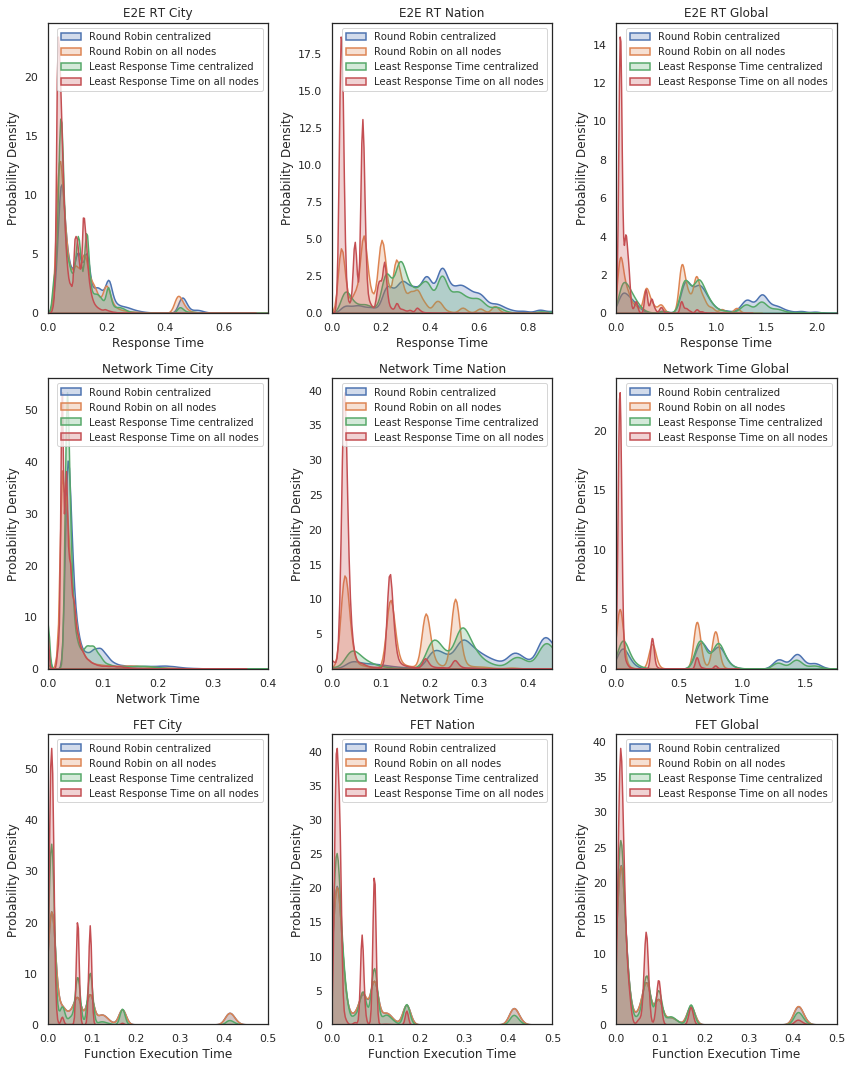
\includegraphics[width=\linewidth]{graphics/graphs/initial_eval_pdfs_3x3.png}
    \caption{\DIFaddFL{Kernel Density Estimate of a single experiment run. Shown data can be interpreted as probability density functions. Data is visualized for \mbox{%DIFAUXCMD
\gls{trt}}\hskip0pt%DIFAUXCMD
, \mbox{%DIFAUXCMD
\gls{fet} }\hskip0pt%DIFAUXCMD
and the time incurred through network transfers.}}
    \label{fig:initial_eval_pdfs}
\end{figure}

\DIFaddend Before developing an approach to the range of engineering challenges such a solution requires we decided to perform a preliminary analysis \DIFdelbegin \DIFdel{in order }\DIFdelend to determine whether distributed \DIFdelbegin \DIFdel{ingress }\DIFdelend \DIFaddbegin \DIFadd{load balancers }\DIFaddend for the serverless system \DIFdelbegin \DIFdel{is }\DIFdelend \DIFaddbegin \DIFadd{are }\DIFaddend a viable solution at all, and if so by how much the performance of network bound workloads can be improved.
To this end we used Faas-Sim\cite{faas-sim-github},
a serverless edge computing simulator built to emulate the core concepts of OpenFaaS and Kubernetes. Building on the work done by Philipp Raith \cite{philipp-da},
we extended the simulator with a more realistic and adaptable method for load \DIFdelbegin \DIFdel{balacing, allowing for different load-balancing }\DIFdelend \DIFaddbegin \DIFadd{balancing, allowing different load balancing }\DIFaddend techniques to be employed, and taking into account function placement and network conditions when simulating requests.%
This preliminary analysis shows an improvement in mean response time of between 81.3\DIFaddbegin \DIFadd{\% }\DIFaddend and 606.9\DIFdelbegin \DIFdel{percent}\DIFdelend \DIFaddbegin \DIFadd{\%}\DIFaddend , depending on the scenario. Fig \ref{fig:initial_eval_pdfs}
shows the fitted probability density functions of the overall response time, function execution time, and network transfer time in different scenarios. From this data we can see that:
\begin{enumerate}
    \item distribution of \DIFdelbegin \DIFdel{ingress points }\DIFdelend \DIFaddbegin \DIFadd{load balancers }\DIFaddend alone is insufficient to improve performance,
    \item more sophisticated \DIFdelbegin \DIFdel{load-balancing }\DIFdelend \DIFaddbegin \DIFadd{load balancing }\DIFaddend methods are required to make use of network proximity, and
    \item sophisticated \DIFdelbegin \DIFdel{load-balancing }\DIFdelend \DIFaddbegin \DIFadd{load balancing }\DIFaddend methods can, in addition to improving network induced delay, reduce function execution time.
    \DIFaddbegin \iitem \DIFadd{The location of load balancers has a significant impact on performance, making the effective placement of load balancers important
}\DIFaddend \end{enumerate}
Based on these results we believe that it is worthwhile to explore this area further, and in more detail than the preliminary evaluation could.


\section{Problem Statement}
% 1 page or less
\DIFaddbegin 

%DIF >  re-state problem of bad performance

%DIF >  re-state our approach of improing the load balancer and placement issue

%DIF >  what problems do we need to solve to improve them
%DIF >  i.e. LB needs to be location aware, potentially FET aware, self-adapting to changes
%DIF >  placement also needs to be location and load aware. Needs to be aware of the different functions, and needs to be aware of the relative differences between topology regions

\DIFadd{Existing serverless and serverless edge computing frameworks still perform worse than expected in certain regards, particularly for network bound workloads where network transfers make up the dominant share of the total processing time\mbox{%DIFAUXCMD
\cite{skippy}}\hskip0pt%DIFAUXCMD
.
This is due to the fact that these frameworks have been built for cloud based environments where the link latency between nodes is small, and the hardware of the nodes themselves homogeneous.
Using these frameworks in an edge scenario as-is leads to requests taking inefficient routes through the network and being processed by a random node, which leads to unnecessarily long network and processing delays.
}

\DIFadd{Based on the results of our initial evaluation we propose that the load balancer implementation, as well as how load balancers are scaled and placed throughout the system needs to be adapted for the edge environment in order to improve the performance of network bound workloads.
}

\DIFadd{For the load balancer implementation itself this means that is has to take into account the heterogeneous nature of nodes the serverless system, the different networking conditions, variable client locations and request rates, as well as the dynamic aspect of edge computing.
The requirements of the load balancer scaling and scheduling component are similar, having to integrate the location of clients, function replicas, existing load balancers, and the request rate into its decisions.
Lastly, both components must be able to handle dynamically changing system conditions, which entails that the makeup of network, devices and clients cannot be known beforehand.
}\DIFaddend \section{Research Questions}

\begin{enumerate}
        \item How \DIFaddbegin \DIFadd{can current scaling and placement techniques for load balancers be changed, such that the overall performance of the serverless edge computing system improves?}\\\\
    \DIFadd{Serverless (edge) computing frameworks typically already possess a mechanism for scaling and placing services. It is also typical for load balancers to be treated as "just another service", and thus identically to functions\mbox{%DIFAUXCMD
\cite{openfaas}}\hskip0pt%DIFAUXCMD
.
    Conceptually this is not surprising since load balancers, like functions, can be scaled to handle more requests than a single instance could.
    Serverless frameworks do not, however, consider the special role load balancers play in the performance of the system in edge computing scenarios.
    To improve the performance, particularly of network bound workloads, the scaling and placement techniques used for load balancers will likely need to be changed. As a result, we need to answer the question how the used techniques in that area have to be adapted in order to realize the aspired performance improvements, while still considering the potential side effects this has on the overall system.
}

        \item \DIFadd{How }\DIFaddend much of a performance improvement can be gained from optimizing the scaling, placement and \DIFdelbegin \DIFdel{routing }\DIFdelend decisions of load balancers in serverless edge computing systems?\\\\
    When investigating what changes could be made \DIFdelbegin \DIFdel{in order }\DIFdelend to increase system responsiveness in serverless edge computing, particularly for network bound workloads, \DIFdelbegin \DIFdel{request routing }\DIFdelend \DIFaddbegin \DIFadd{load balancing }\DIFaddend stands out as an area that is likely to yield significant improvements. Current serverless computing systems do not possess the scaling, placement and \DIFdelbegin \DIFdel{routing mechanisms of load balancers }\DIFdelend \DIFaddbegin \DIFadd{load balancing mechanisms }\DIFaddend required to process requests efficiently in an edge computing scenario. Their implementation is based \DIFdelbegin \DIFdel{around the assumptions }\DIFdelend \DIFaddbegin \DIFadd{on the assumption }\DIFaddend of relative homogeneity in compute power and network structure one typically finds in cloud computing systems. Even serverless computing frameworks specifically built or adapted for the edge do not necessarily take the heterogeneity of edge computing environments into account \DIFdelbegin \DIFdel{. %DIF <  TODO cite here
    }\DIFdelend \DIFaddbegin \DIFadd{when it comes to load balancing\mbox{%DIFAUXCMD
\cite{skippy}}\hskip0pt%DIFAUXCMD
.
    }\DIFaddend This leaves the question of whether or not adapting serverless edge computing frameworks in regard to the scaling and placement of load balancers, \DIFdelbegin \DIFdel{including their routing }\DIFdelend \DIFaddbegin \DIFadd{as well as their load balancing decision }\DIFaddend mechanism, results in performance improvements, and if so, how large they likely are.

        \item How do edge optimized scaling and placement techniques for load balancers, including the load balancing techniques themselves, affect the overall system \DIFdelbegin \DIFdel{behaviour }\DIFdelend \DIFaddbegin \DIFadd{behavior }\DIFaddend and characteristics in regard to their key performance metrics?\\\\
    In a serverless computing framework there usually exists an interplay between a number of different components, such as the scaler and the scheduler\cite{openfaas}\cite{kubernetes}. 
    %DIF < todo check if we need more here
    When parts of the system are now changed, in this case\DIFaddbegin \DIFadd{, }\DIFaddend the way in which load balancers behave, as well as how they are scaled and placed, this change is potentially liable to affect the rest of the system. Some of these effects would of course be intended, such as better end to end latency, but there could also be additional, potentially unwanted effects. It is thus important how exactly such changes affect the system, and what implications that has. These changes are measured in the form of key performance indicators.
\DIFdelbegin %DIFDELCMD < 

%DIFDELCMD <     \item %%%
\item%DIFAUXCMD
\DIFdel{How can current scaling and placement techniques for load balancers be changed, such that the overall performance of the serverless edge computing system improves?}%DIFDELCMD < \\\\
%DIFDELCMD <     %%%
\DIFdel{Serverless (edge) computing frameworks typically already possess a mechanism for scaling and placing services. It is also typical for load balancers to be treated as "just another service", and thus identically to functions\mbox{%DIFAUXCMD
\cite{openfaas}}\hskip0pt%DIFAUXCMD
. 
    In order to improve the performance, particularly of network bound workloads, the scaling and placement techniques used for load balancers will likely need to be changed. As a result we need to answer the question how the used techniques in that area have to be adapted in order to realize the aspired performance improvements, while still considering the potential side effects this has on the overall system.
    }%DIFDELCMD < 

%DIFDELCMD < %%%
\DIFdelend \end{enumerate}
\section{Approach}
% 1 page
Our objective with this thesis is to improve serverless computing for network bound workloads. 
The improvements we aim for are focused primarily on reducing response time, which has already been identified as an issue %DIF < todo cite thomas
\DIFaddbegin \DIFadd{\mbox{%DIFAUXCMD
\cite{skippy}}\hskip0pt%DIFAUXCMD
}\DIFaddend , but are likely also translatable to efficiency gains, depending on what \DIFaddbegin \DIFadd{the }\DIFaddend implementation goals of the specific system in question are.


\DIFdelbegin \DIFdel{We identified request routing }\DIFdelend \DIFaddbegin \DIFadd{Our initial evaluation identified load balancing }\DIFaddend as one of the primary factors holding back the performance of serverless edge computing \DIFdelbegin \DIFdel{, and }\DIFdelend \DIFaddbegin \DIFadd{for network bound workloads, and we }\DIFaddend thus aim to make improvements in this area.
As our preliminary testing showed, the minimum requirements to make meaningful improvements in this area are that \DIFdelbegin \DIFdel{ingress points }\DIFdelend \DIFaddbegin \DIFadd{load balancers }\DIFaddend need to be distributed across the network  instead of being centralized, and that \DIFdelbegin \DIFdel{at those ingress points more sophisticated , context-aware, routing decisionsare made.
In that line }\DIFdelend \DIFaddbegin \DIFadd{they need to make more sophisticated load balancing decisions.
To this end }\DIFaddend our goal is \DIFdelbegin \DIFdel{to explore what effect distributed ingress points and sophisticated load-balancing methods have on the overall system, and to propose }\DIFdelend \DIFaddbegin \DIFadd{two-fold.
First, we want to present }\DIFaddend a method for \DIFdelbegin \DIFdel{load-balancing and placing ingress points within the network that improves overall system }\DIFdelend \DIFaddbegin \DIFadd{scaling and scheduling load balancers in such a way that they are close enough to both clients and function replicas in the network to enable requests to take an efficient path between the two.
Second, we will propose a load balancing scheme that makes load balancing decisions, which take into account the network distance of clients and function replicas, as well as the replicas' }\DIFaddend performance.


To evaluate different approaches for \DIFdelbegin \DIFdel{ingress-placement and load-balancing }\DIFdelend \DIFaddbegin \DIFadd{load balancer placement and load balancing decisions }\DIFaddend we use and extend a state of the art serverless computing simulator, and ground those simulations on real data where possible by building upon existing research%DIF <  cite philipp
\DIFdelbegin \DIFdel{new experiments }\DIFdelend \DIFaddbegin \DIFadd{\mbox{%DIFAUXCMD
\cite{philipp-da}}\hskip0pt%DIFAUXCMD
, and conducting additional experiments to inform the simulator's functioning}\DIFaddend .
This way our methodology allows us to explore scenarios beyond those feasible for live-hardware experimentation, while making sure results are as representative as possible by using performance profiles generated via experiments with actual hardware \DIFdelbegin \DIFdel{.%DIF < todo cite thomas phd thesis
}\DIFdelend \DIFaddbegin \DIFadd{\mbox{%DIFAUXCMD
\cite{thomas-thesis}}\hskip0pt%DIFAUXCMD
.
}\DIFaddend Apart from simulations in the context of serverless computing, we perform separate simulations and experiments in related \DIFdelbegin \DIFdel{and directly relevant }\DIFdelend areas, deepening the understanding \DIFdelbegin \DIFdel{, }\DIFdelend and showing the relation between the challenges of serverless edge computing and the broader context.

We further explore more than just end user performance metrics, also showing how the different components present in modern serverless solutions are influenced and themselves influence methods for \DIFdelbegin \DIFdel{load-balancing and placing ingress points}\DIFdelend \DIFaddbegin \DIFadd{load balancing and placing load balancer replicas}\DIFaddend .
Through this we gain an understanding of, outline, and propose a potential solution for the engineering problems that need to be solved in order to improve serverless edge computing in \DIFdelbegin \DIFdel{practise}\DIFdelend \DIFaddbegin \DIFadd{practice}\DIFaddend .
% Target: 12 pages total: 10ish text, 2ish figures
\chapter{Background}
\section{Serverless Computing}
% got 4 pages
This section aims to give an overview of serverless computing.
Readers who are well-versed within the matter can feel free to skip this introduction, and reference it only when needed
\subsection{What serverless computing is}
Serverless computing, often also referred to as \gls{faas}, emerged as a new computing paradigm in the context of cloud computing.
It is a way in which software developers architect, develop, and deploy applications that is dramatically different from more traditional approaches.
\DIFaddbegin \DIFadd{In traditional approaches, such as microservice architectures, an application is partitioned into small components which can be scaled and deployed independently of each other.
Although microservice architectures often rely on the \mbox{%DIFAUXCMD
\gls{iaas} }\hskip0pt%DIFAUXCMD
solutions cloud providers offer, and thus abstract away the underlying infrastructure to a certain degree, developers still need to handle most scaling and application specific \mbox{%DIFAUXCMD
\gls{qos} }\hskip0pt%DIFAUXCMD
requirements themselves.
}\DIFaddend 

From a developer's perspective\DIFaddbegin \DIFadd{, }\DIFaddend serverless computing is a further increase in abstraction \DIFdelbegin \DIFdel{from developing their applications for bare-metal servers}\DIFdelend \cite{jonasCloudProgrammingSimplified2019}.
It can be seen as the next step in an evolution away from monolithic software applications.
Where microservices and containerized deployments first partitioned a large application into several smaller applications, \DIFdelbegin \DIFdel{each with a distinct set of tasks it performs within the system, }\DIFdelend serverless takes this even further, since in serverless computing applications are partitioned into individual \textit{functions}, which all perform a single action\cite{khandelwalTaureauDeconstructingServerless2020}.

\begin{figure}
    \centering
    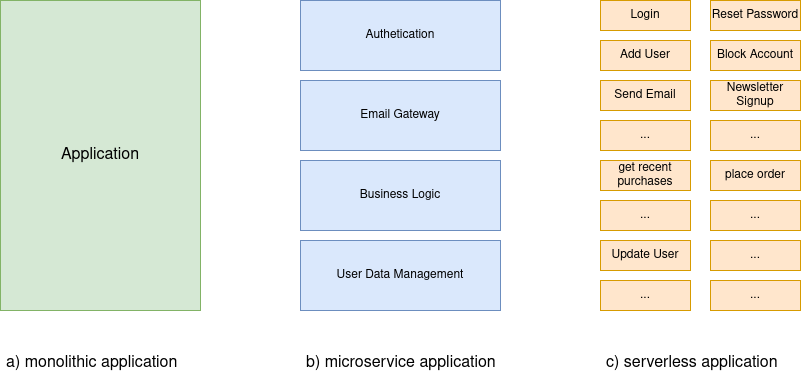
\includegraphics[width=\columnwidth]{graphics/diagrams/monolith_micro_serverless.drawio.png}
    \caption{Conceptual overview of different application architecture paradigms}
    \label{fig:mono_micro_serverless}
\end{figure}

Figure \ref{fig:mono_micro_serverless} shows this transition towards smaller partitioning of application code, leading to a higher and higher level of abstraction.
Just like microservices enabled application developers to scale different aspects of an application independently, thus enabling elasticity, serverless computing takes this even further allowing individual functions of the application to be scaled \DIFdelbegin \DIFdel{independently}\DIFdelend \DIFaddbegin \DIFadd{separately from each other}\DIFaddend \cite{jonasCloudProgrammingSimplified2019}.

Overall serverless affords application developers a number of advantages:
\begin{itemize}
    \item \textbf{Arbitrary elasticity:} As mentioned, serverless applications can scale their components on an extremely fine-grained level\cite{khandelwalTaureauDeconstructingServerless2020}
    \item \textbf{Abstracted infrastructure:} Where previously developers needed to be at least somewhat cognizant of the deployment of their application or its microservices, serverless enables this task to be fully delegated to the cloud provider. Developers don't necessarily need any knowledge of cloud infrastructure\cite{jonasCloudProgrammingSimplified2019}.
    \item \textbf{Precise Billing:} While in traditional cloud computing environments resources are leased for a set amount of time, irrespective of their actual usage\cite{khandelwalTaureauDeconstructingServerless2020}, serverless features a billing model where only the actual execution time and memory footprint of a function is billed down to millisecond precision\cite{jonasCloudProgrammingSimplified2019}. This allows for better resource utilization and potentially reduced costs from a customer's perspective\cite{khandelwalTaureauDeconstructingServerless2020}.
\end{itemize}

While these advantages of serverless computing over more traditional approaches are compelling, there are also idiosyncrasies of serverless computing that, depending on the application, be problematic.
These include the need for statelessness, meaning that serverless functions have no inherent capacity to store data and would instead need to fetch it from yet another service\cite{khandelwalTaureauDeconstructingServerless2020}, or potential performance inconsistencies from cold-starts.
A cold-start, which means that the specific function code isn't running and has to be started before the request can be serviced, can occur because a serverless function wasn't executed for a certain time\cite{wangPeekingCurtainsServerless2018}.

\subsection{The architecture of serverless systems}
Architecturally, serverless systems are closely related to \DIFdelbegin \DIFdel{even }\DIFdelend \DIFaddbegin \DIFadd{event }\DIFaddend based systems.
Their general concept is also very similar, since an event (i.e. a request) first arrives at the system in a form of queue, where a dispatcher \DIFaddbegin \DIFadd{or load balancer }\DIFaddend decides what action needs to be taken based on the event, and forwards it to the service (i.e. function), which ultimately processes it\cite{castroServerDeadLong2019}.

Prominent cloud based serverless platforms such as AWS Lambda\cite{aws-lambda} and Azure Functions\cite{azure-functions} are, however, proprietary and their precise architecture and inner workings are thus unknown to the public.
How these systems behave is a topic of ongoing research\cite{wangPeekingCurtainsServerless2018}, but since our research requires precise knowledge of implementation details, we choose to use open source serverless frameworks as a reference architecture of serverless systems.
These systems include Apache OpenWhisk\cite{openwhisk}, Kubeless\cite{kubeless}, and OpenFaaS\cite{openfaas}.
Since OpenFaaS has already been adapted for serverless edge computing by Rausch et al.\cite{rauschServerlessPlatformEdge}, we choose to use this open source serverless framework as the stand-in for serverless computing frameworks in general.

Architecturally, OpenFaaS is structured very similarly to the generic serverless architecture described by Castro et al.\cite{castroServerDeadLong2019}.
It too has a centralized entry-point, the Gateway, which sends requests to specific function replicas or alternatively to a queue (used for asynchronous processing and dealing with requests to functions that aren't currently running).
Figure \ref{fig:openfaas-gateway-diagram} shows a diagram of the architecture, as it is found in their official documentation\cite{openfaas-gateway}.

From a technical perspective\DIFaddbegin \DIFadd{, }\DIFaddend a key aspect of OpenFaaS' implementation is that it uses containers to host functions.
Containers provide an abstraction over Linux based operating systems, allowing for easier management of software dependencies, more closely controlled execution environments, and stronger application isolation.
Each function is packaged into such a container, which is an almost fully self-contained and portable artifact, that allows executing the developers\DIFaddbegin \DIFadd{' }\DIFaddend code on any machine with a compatible container runtime.
Functionally they behave similar to virtual machines, although they start up much faster, and aren't actually running individual kernels, which is why they do not provide the same level of security isolation true virtual machines do.
This choice allows functions to execute reliably, no matter the environment, and also makes it entirely agnostic to the programming language developers wish to use.
Since using containers entails their management over a cluster of multiple nodes, a task which is extremely complex, OpenFaaS\DIFdelbegin \DIFdel{builds upon }\DIFdelend \DIFaddbegin \DIFadd{\mbox{%DIFAUXCMD
\cite{openfaas} }\hskip0pt%DIFAUXCMD
as well as other serverless frameworks build on }\DIFaddend Kubernetes\cite{kubernetes}, \DIFdelbegin \DIFdel{a full-featured }\DIFdelend \DIFaddbegin \DIFadd{the de-factor industry default }\DIFaddend container orchestration and management platform.
Building upon Kubernetes to deal with container management is a common choice among open source serverless frameworks, a choice which OpenWhisk and Kubeless make as well\cite{mohantyEvaluationOpenSource2018}.

OpenFaaS delegates a large number of tasks to the underlying Kubernetes cluster, including name resolution, request routing, \DIFaddbegin \DIFadd{which includes load balancing, }\DIFaddend and potentially scaling.
For this work\DIFaddbegin \DIFadd{, }\DIFaddend the delegation of \DIFdelbegin \DIFdel{request routing }\DIFdelend \DIFaddbegin \DIFadd{load balancing decisions }\DIFaddend is especially important, since it implies that OpenFaaS uses whichever load balancing algorithm Kubernetes uses internally to distribute requests among function replicas.
Scaling, which determines how many instances of a serverless functions are running at any given time, can work via different mechanisms in OpenFaaS.
Depending how OpenFaaS is configured, it can either use Kubernetes' integrated \gls{hpa}\cite{kubernetes-hpa} or its own internal mechanism, which \DIFdelbegin \DIFdel{allows for a }\DIFdelend \DIFaddbegin \DIFadd{optionally allows for }\DIFaddend user customized scaling \DIFdelbegin \DIFdel{behaviour}\DIFdelend \DIFaddbegin \DIFadd{behavior}\DIFaddend \cite{openfaas-autoscaling}.
Since this work also aims to explore the impact a change in scaling and scheduling load balancers can have on the \DIFdelbegin \DIFdel{behaviour }\DIFdelend \DIFaddbegin \DIFadd{behavior }\DIFaddend of these scaling systems in general, we will now briefly describe the default scaling \DIFdelbegin \DIFdel{behaviour }\DIFdelend \DIFaddbegin \DIFadd{behavior }\DIFaddend of both \gls{hpa} and OpenFaaS\DIFdelbegin \DIFdel{integrated solution}\DIFdelend \DIFaddbegin \DIFadd{' own scaler}\DIFaddend .

\subsubsection{Kubernets \gls{hpa}}
In Kubernetes scaling is typically based on either CPU or memory utilization, although in principle it can be \DIFdelbegin \DIFdel{extrended }\DIFdelend \DIFaddbegin \DIFadd{extended }\DIFaddend with user-provided custom metrics\cite{kubernetes-hpa}.
For a given deployment, which in the context of serverless computing would be a function, a target resource value is defined.
An example would be a target average CPU utilization of 50\% for a type of function.
At that point\DIFaddbegin \DIFadd{, }\DIFaddend Kubernetes decides in a linear fashion what the desired number of replicas is.
\DIFaddbegin 

\DIFadd{Let $\mathbf{r_{\text{current}}}$ be the number of current replicas, $\mathbf{m_{\text{current}}}$ the current value of the metric in question and $\mathbf{m_{\text{target}}}$ the target value of the metric.
Then the target replica count is
}

\DIFaddend \[ \DIFdelbegin \DIFdel{\text{Let } }\DIFdelend r\DIFaddbegin \DIFadd{_{\text{target}} = }\left \lceil \DIFadd{r}\DIFaddend _{\text{current}} \DIFdelbegin \DIFdel{\text{ be the number of current replicas, }}\DIFdelend \DIFaddbegin \DIFadd{\times \frac{m_{\text{current}}}{m_{\text{target}}} }\right \rceil\DIFaddend \]
\DIFdelbegin \[\DIFdel{m_{\text{current}} \text{ the current value of the metric in question}}\]%DIFAUXCMD
\[\DIFdel{\text{ and } m_{\text{target}} \text{ the target value of the metric. Then the target replica count is }}\]%DIFAUXCMD
\[ \DIFdel{r_{\text{target}} = \left \lceil r_{\text{current}} \cdot \frac{m_{\text{current}}}{m_{\text{target}}} \right \rceil}\]%DIFAUXCMD
\DIFdelend 

To prevent inconsistent \DIFdelbegin \DIFdel{behaviour }\DIFdelend \DIFaddbegin \DIFadd{behavior }\DIFaddend such as replica counts oscillating Kubernetes also allows certain limiters to be set, such as minimum and maximum scales, rate of change for adding or removing replicas, and cool-downs which \DIFdelbegin \DIFdel{allow the system }\DIFdelend \DIFaddbegin \DIFadd{give the system time }\DIFaddend to stabilize before new scaling decisions are considered\cite{kubernetes-hpa}.

\subsubsection{OpenFaaS \DIFdelbegin \DIFdel{integrated }\DIFdelend scaling}
The OpenFaaS integrated scaling mechanism is comprised of different parameters.
First a minimum and maximum scale must be set, which determine the effect of the scaling factor.
In this custom scaling variant system parameters, such as the request rate of a given function, are continuously evaluated.
Once a configured condition is met the system is notified that a given function needs to scale up or down.
The aforementioned scaling factor, which is a percentage value between 0 and 100, is then used to determine how many replicas should be started or stopped\cite{openfaas-autoscaling}.
Each scaling \DIFdelbegin \DIFdel{iterations }\DIFdelend \DIFaddbegin \DIFadd{iteration }\DIFaddend adds or removes a number of replicas relative to the maximum scale allowed, and the scaling factor determines the size of that share.
If, for example, the maximum number of replicas is 50, and the scaling factor is 10\%, then at each scaling operation 5 replicas will be added or removed.

Which exact conditions trigger a scale up or scale down event within OpenFaaS is extremely configurable, and allows for customization based on an individual \DIFdelbegin \DIFdel{functions }\DIFdelend \DIFaddbegin \DIFadd{function's }\DIFaddend requirements.
By default\DIFaddbegin \DIFadd{, }\DIFaddend OpenFaaS triggers a scale-up event if the rate of rise of a \DIFdelbegin \DIFdel{functions }\DIFdelend \DIFaddbegin \DIFadd{function's }\DIFaddend invocation frequency exceeds a threshold over a period of time.




\section{Serverless Edge Computing}
% give a brief introduction to edge computing, just what it is + the obligatory graphic.
% what is serverless edge computing then?
% why don't current systems work well on the edge?
% give example of what it is necessary for -> edge intelligence, the bunch of applications that I've gathered, etc.
% about 2 pages should do just nicely

Serverless edge computing is an extension of existing serverless computing frameworks to the edge of the network.
It is an area of ongoing research, and aims to both further the adoption of edge computing and enable new use cases\cite{nasticServerlessRealTimeData2017}.

\subsection{Edge Computing}
Edge Computing has been proposed as a new computing paradigm to address a number of limitations and shortcomings of centralized cloud computing.
Edge Computing means that computations are not performed in a \DIFdelbegin \DIFdel{singe }\DIFdelend \DIFaddbegin \DIFadd{single }\DIFaddend centralized location like a data center, but close to where the computations are needed or requested from, i.e. the edge of the network\cite{shiPromiseEdgeComputing2016}.

\begin{figure}
    \centering
    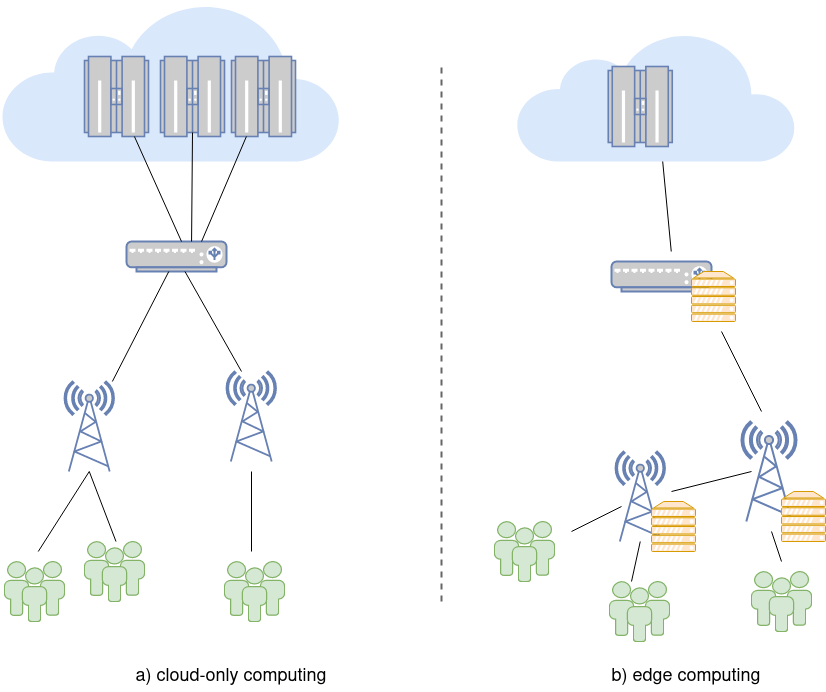
\includegraphics[width=12cm]{graphics/diagrams/edge_computing_example.png}
    \caption{An example of how in b) edge computing there are nodes interspersed throughout the network and close to clients, while in a) cloud computing all computation is centralized.}
    \label{fig:edge_comp_example}
\end{figure}

Edge computing enables a number of structural benefits that allow for the creation of new types of use-case and application.
Most notably, edge computing enables low latency, high bandwidth, computation offloading.
This can be used to improve application responsiveness, perform computations not possible on low-powered devices \DIFdelbegin \DIFdel{, }\DIFdelend or conserve energy on mobile devices by offloading complex computations to nearby edge nodes\cite{abbasMobileEdgeComputing2018b}.
Edge computing can also been seen as a way to transparently improve cloud computing, reducing the overall traffic in the network and making existing cloud applications more responsive by moving them closer to the user\cite{satyanarayananEmergenceEdgeComputing2017}.
Figure \ref{fig:edge_comp_example} shows the \DIFdelbegin \DIFdel{different }\DIFdelend \DIFaddbegin \DIFadd{difference }\DIFaddend between edge and cloud computing in a simplified way.
In the example\DIFaddbegin \DIFadd{, }\DIFaddend edge computing features computational nodes on \gls{ran}-towers, and thus much closer to the users.


This computing paradigm does, however, \DIFdelbegin \DIFdel{have a number of characteristics that make it different from cloud computing and }\DIFdelend pose a challenge to existing frameworks and application architectures.
Given that computation resources are spread  farther throughout the network, the network infrastructure itself in edge computing is much more diverse\cite{shiEdgeComputingVisionChallenges2016}, potentially consisting of anything from the unreliable mobile network connection of a user's device to high bandwidth fiber networks between cloud data centers.
From both a hardware and software perspective, the computation hardware itself is more heterogeneous as well, requiring specific optimization mechanism to use resources in the most efficient way possible\cite{abbasMobileEdgeComputing2018b}.

\subsection{Serverless at the Edge}
Since serverless computing offers an abstraction layer on top of the actual infrastructure \cite{jonasCloudProgrammingSimplified2019}, and a key challenge of edge computing is that edge applications, at least up to now, have to be specifically crafted for their deployment scenario by developers\cite{shiPromiseEdgeComputing2016}.

With future \gls{ai} applications being dependent on edge computing to deliver their benefits to users via augmented reality, and smart city infrastructure\cite{rauschEdgeIntelligenceConvergence2019}, serverless offers an attractive abstraction layer to develop such \gls{ai} applications in an edge-native way.
Building on serverless as an abstraction layer for the application, the idea is that it will be able to jointly provide the benefits afforded by edge computing and serverless computing at the same time.
Functions are supposed to be deployed to nodes close to the users that rely on these functions, be scaled automatically, and routed efficiently, without any manual intervention from developers.

Achieving such a computing infrastructure would enable a host of new types of application, such as wearable cognitive assistance\cite{haWearableCognitiveAssistance2014}\cite{rauschPlatformSmartCityScale2021}, offloading \gls{ai} inference tasks from devices with low compute capability\cite{liEdgeAIOnDemand2020}, and analyzing video feeds in real time to improve public safety\cite{zhangEdgeVideoAnalytics2019}, for example\DIFaddbegin \DIFadd{, }\DIFaddend to ensure face masks are worn where mandated\cite{wangWearMaskFastInbrowser2021}.

Open source serverless frameworks have been evaluated in terms of their performance in edge-scenarios, but in their current, unmodified state they lack the full set of capabilities needed to provide all the benefits edge computing offers\cite{paladeEvaluationOpenSource2019}.
While some of these serverless frameworks have been adapted to address the challenges posed by the edge computing environment, or to be better tailored to workloads related to \gls{ai}\cite{rauschServerlessPlatformEdge}, more of which will be discussed in the next chapter, overall there remain a lot of challenges for the universal practical application of serverless edge computing\cite{aslanpourServerlessEdgeComputing2021}.
Optimizing the performance of network bound workloads, for example, is one such challenge\cite{skippy}, and the one this thesis aims to address.




\section{Load Balancing}
Load balancing refers to the concept of distributing \DIFdelbegin \DIFdel{the load, which can be any arbitrary task, but is typically a web request, between different server }\DIFdelend \DIFaddbegin \DIFadd{requests between different servers }\DIFaddend in such a way that \DIFdelbegin \DIFdel{they }\DIFdelend \DIFaddbegin \DIFadd{the amounts of requests per server }\DIFaddend are balanced.
It is a necessary component of a system where a single instance cannot service all requests, and thus multiple instances are used to keep performance levels acceptable.
\DIFdelbegin \DIFdel{What exactly constitutes a }\DIFdelend \DIFaddbegin \DIFadd{A }\DIFaddend balanced distribution can depend on one's objectives, but typically \DIFdelbegin \DIFdel{a balanced distribution is one that maximizes }\DIFdelend \DIFaddbegin \DIFadd{aims to maximize }\DIFaddend overall system performance over the available servers\cite{cardelliniDynamicLoadBalancing1999a}.

While load balancer type system components are ubiquitous in our modern computing environment, in \DIFdelbegin \DIFdel{the context of }\DIFdelend this work we focus solely on web load balancers.
From the perspective of the OSI network reference model\cite{dayOSIReferenceModel1983}, load balancers typically work on the transport layer (level 4), or the application layer (level 7).
Because serverless frameworks like OpenFaaS differentiate between functions based on HTTP request data, only \DIFdelbegin \DIFdel{application level }\DIFdelend \DIFaddbegin \DIFadd{application-level }\DIFaddend load balancing is of concern for us in the context of this paper.

There exist a large number of load balancing algorithms, which decide the application instances servicing each request.
The most common algorithms include:
\begin{itemize}
    \item \textbf{Round Robin:} requests are distributed evenly between servers, irrespective of the performance or load of each server. Each subsequent request is sent to a different server.
    \item \textbf{Weighted Round Robin:} requests are also distributed among servers, but not necessarily evenly. Each server is manually assigned a weight, which determines the share of requests it receives relative to other servers. Weights scale linearly, meaning that one server having double the weight of another also means that it will receive double the requests
    \item \textbf{Least Response Time:} can be implemented in different ways. In the naive approach the load balancer forwards all requests to the server showing the fastest initial response time, until that \DIFdelbegin \DIFdel{servers }\DIFdelend \DIFaddbegin \DIFadd{server's }\DIFaddend performance degrades to the point where another server is faster, which receives subsequent requests from that point on.
\end{itemize}

Since OpenFaaS\cite{openfaas} builds on Kubernetes and its primitives, it also delegates service resolution and thus request routing to it.
While Kubernetes can use any type of load balancer in principle, particularly the kinds available from cloud providers as a managed service, it defaults to using \DIFdelbegin \DIFdel{it's }\DIFdelend \DIFaddbegin \DIFadd{its }\DIFaddend internal kube-proxy to handle traffic routing, which in turn defaults to using a round robin load balancing strategy.
Next, we elaborate on the role load balancing plays in serverless frameworks in a bit more detail.


\subsection{ Definition \& Role In a Typical Serverless Framework}
To give a bit more context to the role of load balancers in this work, we now discuss what component exactly we mean by \textit{load balancer}, and how it functions in the context of a serverless framework. While our approach is not tied to any specific serverless framework, implementation, or technology, we developed it with their general concepts and functioning in mind. Because of this\DIFaddbegin \DIFadd{, }\DIFaddend we feel that is helpful and informative to explain the components of our system in the context of an actual implementation, since this helps understand the abstract role these components play. In addition\DIFaddbegin \DIFadd{, }\DIFaddend this is helpful for anyone who might want to integrate our approach into a production ready serverless edge computing platform.

As previously mentioned there are a number of different serverless frameworks, some free, some open source, some commercial, and some that fall in-between\cite{aws-lambda}\cite{azure-functions} \cite{openfaas-gateway}\cite{kubeless}\cite{openwhisk}.
To reiterate, we choose OpenFaaS as a proxy for serverless computing frameworks in general because it has been extended for edge computing, and because it builds on and makes use of well established technologies in the same way other serverless frameworks do\cite{kubeless}\cite{openwhisk}, thus making it representative for the space.


\begin{figure}
    \centering
    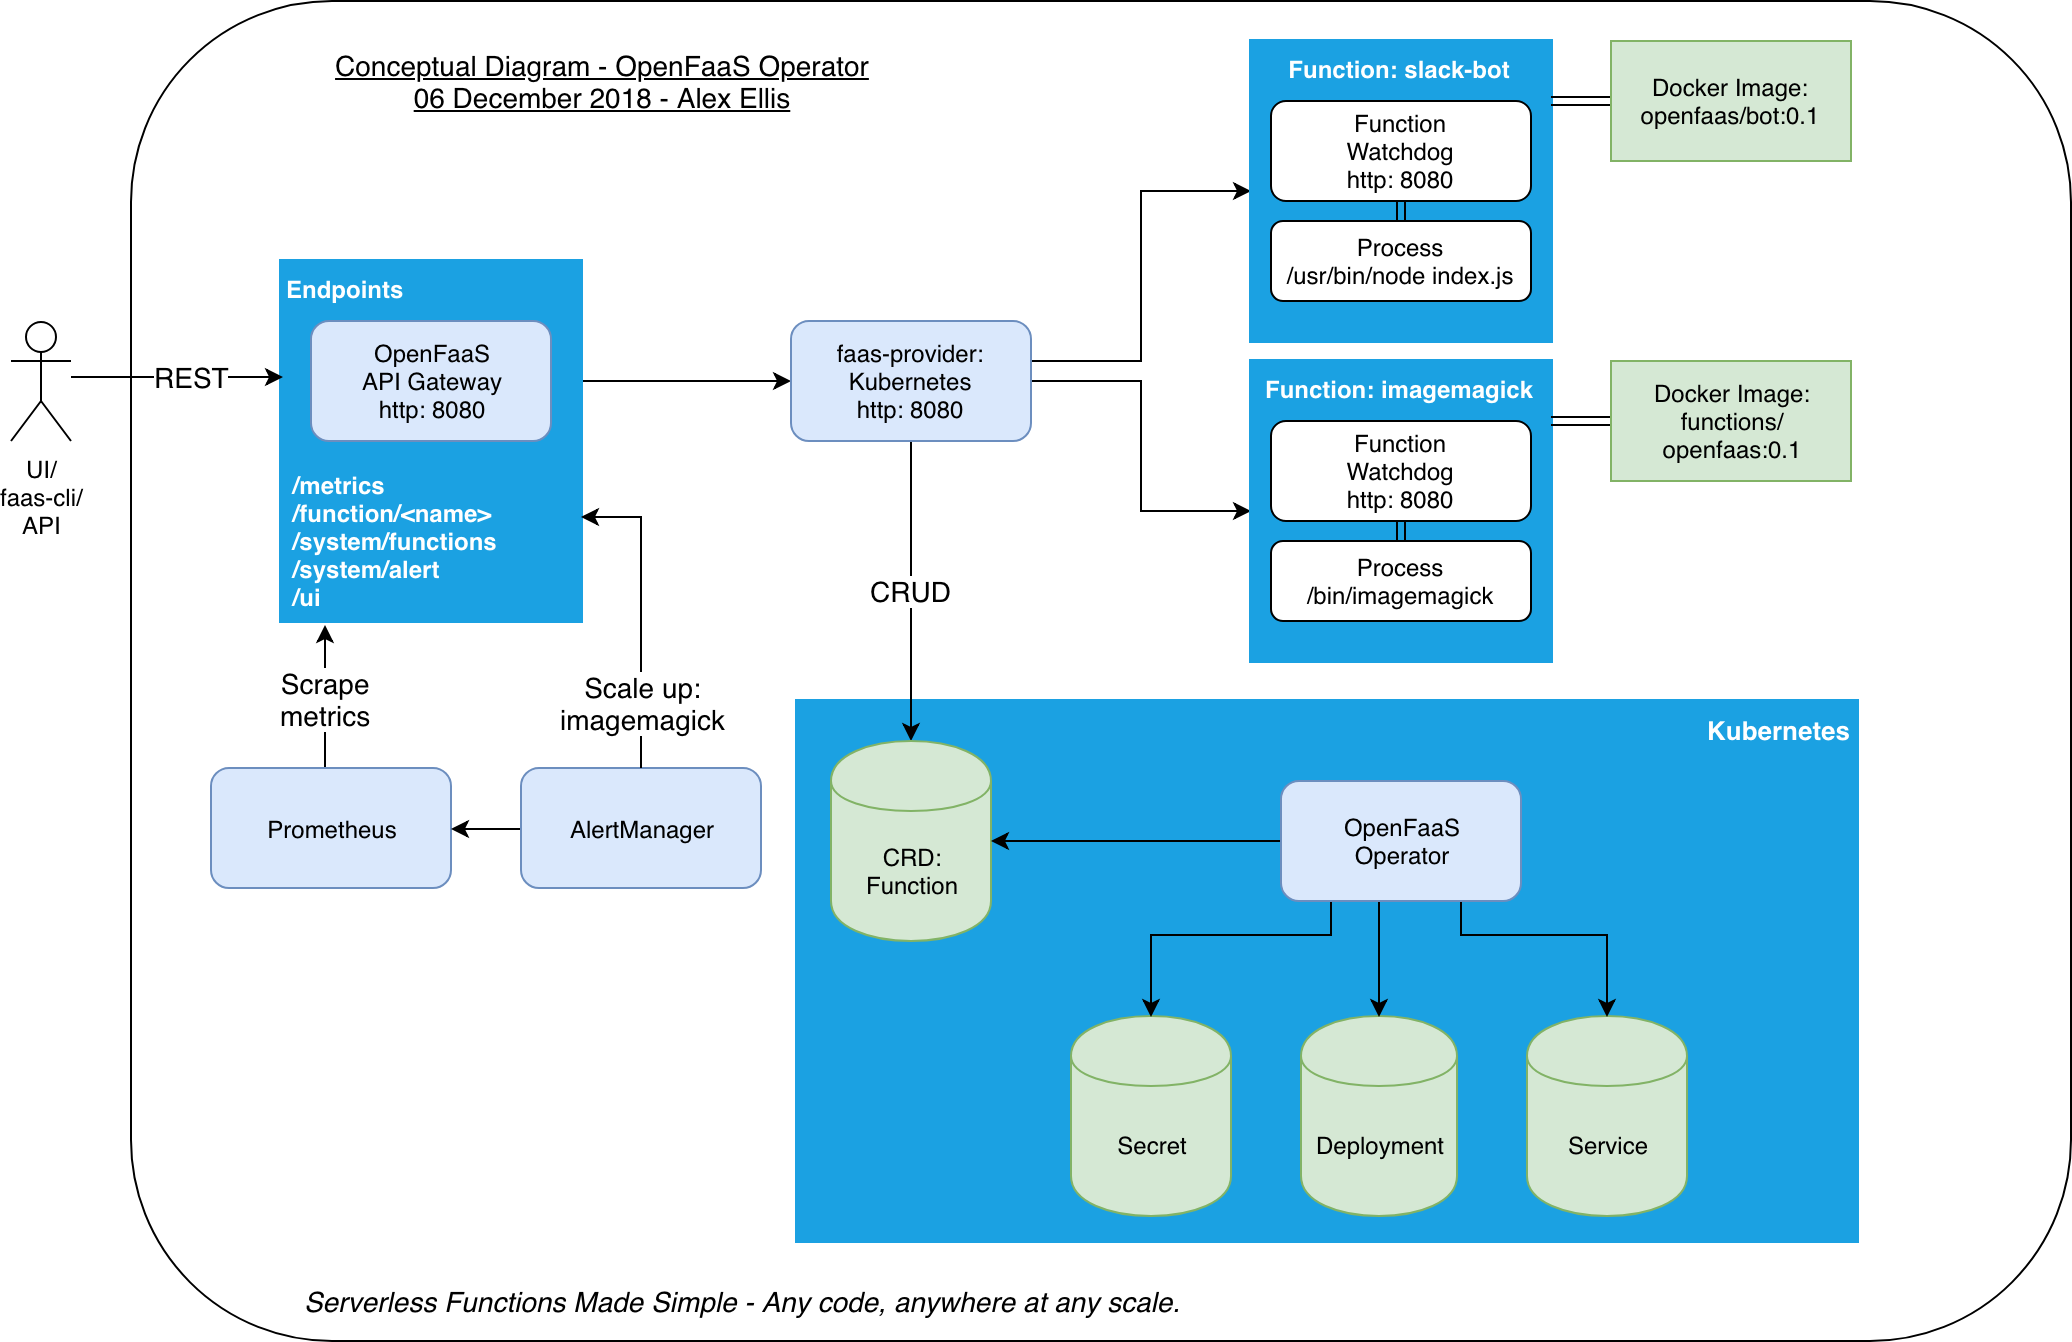
\includegraphics[width=14cm]{graphics/diagrams/openfaas-gateway-architecture.png}
    \caption{Diagram showing the architecture and components of OpenFaaS, in particular the OpenFaaS API Gateway. Taken from the official OpenFaaS architecture documentation\cite{openfaas-gateway}}
    \label{fig:openfaas-gateway-diagram}
\end{figure}


As mentioned, OpenFaaS uses Linux containers to run functions, and in turn Kubernetes to manage these containers. To clarify the role our load balancer would take in a serverless system, we describe how it would affect OpenFaaS. By default\DIFaddbegin \DIFadd{, }\DIFaddend OpenFaaS employs a component they call \textit{API Gateway}. This API Gateway is the component \DIFdelbegin \DIFdel{which }\DIFdelend \DIFaddbegin \DIFadd{that }\DIFaddend first receives \textbf{all} client requests, and then continues to send them on to the corresponding functions, while at the same time collecting metrics used by the system for tasks like auto-scaling. Figure \ref{fig:openfaas-gateway-diagram}, which is taken directly from the official OpenFaaS documentation shows the interactions with the other components of the system. Since the API Gateway is just another container running in Kubernetes\cite{kubernetes}, and failover capability is a concern, there can be multiple instances of the API Gateway running at any given time.
As discussed a major reason for the sub-optimal performance of network bound workloads in edge scenarios is the lack of efficient request routing.
In the case of OpenFaaS this stems from it delegating networking and routing tasks to Kubernetes, since it is the underlying container orchestration platform. This applies to both the initial ingress into the cluster, as well as to how the API Gateway forwards client requests to the relevant replicas to be processed. Kube-proxy, the component of Kubernetes which handles networking and routing tasks, will default to the round-robin policy of selecting upstreams. While it is possible to set up kube-proxy in a way that will prefer nodes in the same zone based on a label, this functionality is built around cloud based deployments and is insufficient to address the heterogeneity in networking and compute power introduced by edge computing. This defaulting to round-robin means that in effect, serverless frameworks such as OpenFaaS route the requests basically at random between the entry point of the network and the API Gateway, and then from the API Gateway to the relevant function.\\
In our approach\DIFaddbegin \DIFadd{, }\DIFaddend the load balancer takes the role the API Gateway has in OpenFaaS. It is characterized by being
\begin{enumerate}
    \item the entry point for the client to the serverless system, meaning there are no network hops between the load balancer instance and the node the request originally arrived at, and
    \item directly forwarding requests to the corresponding serverless function instances.
\end{enumerate}
When implementing our proposed approach in \DIFdelbegin \DIFdel{practise }\DIFdelend \DIFaddbegin \DIFadd{practice }\DIFaddend this would mean that the serverless framework would have to be adapted to fulfill these conditions for the load balancer. If these conditions aren't met, this would likely negate the positive \DIFdelbegin \DIFdel{affect }\DIFdelend \DIFaddbegin \DIFadd{effect }\DIFaddend our approach has on performance.

As an example in the case of OpenFaaS, referencing the OpenFaaS architecture in Figure \ref{fig:openfaas-gateway-diagram}, this could be realized in the following ways:
\begin{enumerate}
    \item API Gateways and load balancers are scaled and scheduled together, meaning they are always co-located on the same node. The API-Gateway would then still first receive requests and handle \DIFdelbegin \DIFdel{implementation specific }\DIFdelend \DIFaddbegin \DIFadd{implementation-specific }\DIFaddend tasks for the serverless system, but then forward the request to the load balancer instance on the same node, which then decides on further request routing.
    \item The load balancer is the new entry point for clients, effectively replacing the API Gateway. In this scenario\DIFaddbegin \DIFadd{, }\DIFaddend the load balancer and API Gateway would also be altered such that metrics and information relevant to the system could be collected by the load balancers and forwarded to API Gateway instances, which then handle them as before.
\end{enumerate}
\section{Service Placement}
% 0,5 - 1 page
% just explain how containers are scheduled in kubernetes by default
% just the general concept of matching with resources and resource reservation concept.
% mention that there are works that aim to improve these decisions, but this should be short and to the point
Service placement, in the context of this work, refers to how instances of an application or application component are placed within a cluster or network.
Referring specifically to serverless computing, once the scaler has determined new replicas of a function have to be created, the scheduling component then decides where the new replicas, i.e. the service, should be placed.
As open source serverless frameworks rely on Kubernetes to handle these types of container orchestration tasks\cite{mohantyEvaluationOpenSource2018}, the Kubernetes scheduler effectively decides where function replicas are placed.

Generally, Kubernetes uses a \DIFdelbegin \DIFdel{two stage }\DIFdelend \DIFaddbegin \DIFadd{two-stage }\DIFaddend process for deciding where a new replica is placed.
In the first step all nodes in the cluster are filtered, to leave only the ones that meet the basic requirements of running the replica in question.
Typically that includes available CPU time, free memory, and other conditions such as the required ports being available on the node.
Remaining nodes are then ranked according to a set of default, and optionally custom specified, scoring methods.
The node with the highest score is then selected to host the new replica.

While this is only a very basic overview, it helps to understand the \DIFdelbegin \DIFdel{behaviour }\DIFdelend \DIFaddbegin \DIFadd{behavior }\DIFaddend of serverless systems, and how our approach could be integrated into open source serverless frameworks.

% Target: 5ish pages of text
\chapter{Related Work}

\section{Serverless Edge Computing}
Glikson, Nastic, and Dustdar first propose serverless edge computing under the name \textit{deviceless edge computing} to the transparent infrastructure abstraction serverless computing provides to the edge\cite{gliksonDevicelessEdgeComputing2017}.
Nastic et al. exemplify this concept through their proposal of an analytics platform for real-time data using serverless edge computing\cite{nasticServerlessRealTimeData2017}.
They provide use cases for which such a platform would be beneficial, and present an architectural view outlining the components needed.
In addition\DIFaddbegin \DIFadd{, }\DIFaddend they elaborate on the challenges the edge poses for such a system, particularly heterogeneity in resources and infrastructure, and data management\cite{nasticServerlessRealTimeData2017}.
Aslanpour et al. round out the conceptual understanding of serverless edge computing by outlining the current vision and challenges of the space \cite{aslanpourServerlessEdgeComputing2021}.
Among the challenges listed are resources inefficiency, distributed networking, location agnosticism, and a lack of simulation tools\cite{aslanpourServerlessEdgeComputing2021}, all of which we hope to contribute \DIFdelbegin \DIFdel{in }\DIFdelend \DIFaddbegin \DIFadd{to }\DIFaddend overcoming with the work presented in this thesis.

Rausch et al.\cite{rauschServerlessPlatformEdge} present the architectural considerations necessary to bring \gls{ai} applications to the edge using serverless computing.
Parts of the life cycle of an \gls{ai} application make their deployment in serverless edge systems a particular challenge\cite{aslanpourServerlessEdgeComputing2021}, which Rausch et al. address by giving application developers more fine-grained control over scheduling decisions\cite{rauschServerlessPlatformEdge}, who can formulate constraints to guarantee deployments of their \gls{ai} application have the resources they need available, even at the edge.
Putting the proposition of these constraints into practice Rausch et al. present a scheduler which is able to consider such resource and locality constraints\cite{skippy}.
Rausch et al. show that their scheduler makes significantly better scheduling decisions than the default Kubernetes scheduler, using the resources in a more efficient manner and reducing \gls{fet}\cite{skippy}. \DIFaddbegin \DIFadd{In contrast to this work, they do not consider the load balancing component of the system as something to be scaled and scheduled separately from the other functions.
}\DIFaddend 

Cicconetti et al. propose different methodologies for matching up clients with function replicas in a serverless system\cite{cicconettiDistributedComputingEnvironments2020}.
They evaluate different assignment policies, showing through simulations that between static global matching, periodical global matching, and dynamic decentralized matching of clients to replicas, the decentralized version performs best.
Their work is closely related to ours in that it too explores ingress points at the edge.
\DIFaddbegin \DIFadd{Functionally, their notion of ingress points, or dispatcher as they call it, is identical to what we in this work refer to as a load balancer.
They do not, however, discuss how these dispatcher components are placed throughout the network, which is a significant difference from our work.
Additionally, their conceptual view of the system differs from ours in that they assume clients to be assigned to dispatchers by a centralized orchestration component, while we work on the assumption that clients are connected to whichever load balancer is closest at the time of the request being sent.
}\DIFaddend In subsequent work Cicconetti, Conti and Passarella\cite{cicconettiArchitecturePerformanceEvaluation2020} explore the idea of building a performance model for function replicas, both in terms of \gls{fet} and network time, to account for the heterogeneity found in edge systems.
In another paper, which strongly intersects with this work, Cicconetti, Conti, and Passarella explore methods for distributed load balancing\cite{cicconettiDecentralizedFrameworkServerless2020}.
In their experiments, their proposed version of selective weighted round robin load balancing outperforms naive least response time load balancing, and random weighted round robin load balancing.
\DIFaddbegin \DIFadd{While similar to our approach in that a combination of weighted round robin and least response time is used to make load balancing decisions, our approach differs from theirs in the way upstreams are sampled and weights are assigned.
They assume a cutoff at twice the optimum performance, meaning upstreams that show a response time more than double the optimum do not receive requests for a given time period, while we do not assume such a cutoff\mbox{%DIFAUXCMD
\cite{cicconettiDecentralizedFrameworkServerless2020}}\hskip0pt%DIFAUXCMD
.
Which approach is better in this regard will depend on the particular scenario of the evaluation.
Another difference is that their weight assignments are linearly proportional to the response time, while in our approach a factor can be defined that determines whether this relationship is linear, logarithmic, or exponential.
}\DIFaddend 


Baresi and Mendonca\cite{baresiServerlessPlatformEdge2019} address a range of engineering challenges that need to be solved for serverless edge computing, focusing particularly on function composition, challenges of stateful computations, and potential protocol overhead.

Lastly, Gadepalli et al. \cite{gadepalliChallengesOpportunitiesEfficient2019} propose aWsm, a serverless edge computing platform focused around the advantages afforded by using Web Assembly as a basis.
Their work places a particular emphasis on execution efficiency, meaning a low memory footprint, and fast start-up times to address the cold-start problems endemic to serverless platforms, and one of the challenges for serverless edge computing outlined by Aslanpour et al.\cite{aslanpourServerlessEdgeComputing2021}.


\section{Load Balancing at the Edge}
% got 2 pages
Load Balancing is a topic that is well established and studied in the scientific literature.
Edge compute introduces several challenges to established load balancing algorithms, in particular through resource and network heterogeneity\cite{gardnerScalableLoadBalancing2021}.

A number of researchers propose adaptations of the well known \gls{jsq} and \gls{jiq} load balancing techniques to overcome some or all of these challenges\cite{gardnerScalableLoadBalancing2021}\cite{wengOptimalLoadBalancing2020}\cite{vargaftikLSQLoadBalancing2020}.
Gardner et al. propose a to adapt \gls{jiq} and \gls{jsq} by changing how the upstream queue lengths are sampled.
Instead of sampling the queue length of all nodes, which in and of itself can be infeasible in large systems\cite{gardnerScalableLoadBalancing2021}, their implementation considers two subsets of nodes.
One is drawn from a set of nodes determined to be fast, while the other is drawn from a subset determined to be slow.
The relative performance level of nodes and thus their categorization is assumed to be a priori knowledge.

In a different approach to \DIFdelbegin \DIFdel{address }\DIFdelend \DIFaddbegin \DIFadd{addressing }\DIFaddend the issue of large clusters, where not all nodes can be sampled, Vargaftik, Keslassy, and Orda propose that load balancers hold a local view of server queues, which \DIFdelbegin \DIFdel{isn't }\DIFdelend \DIFaddbegin \DIFadd{is not }\DIFaddend fully updated all the time\cite{vargaftikLSQLoadBalancing2020}.
While all nodes in the local view of the system state are considered for load balancing, only a small subset of all nodes \DIFdelbegin \DIFdel{is }\DIFdelend \DIFaddbegin \DIFadd{are }\DIFaddend queried for their actual queue length at a given iteration.

Weng, Zhou and Srikant propose adapted versions of \gls{jiq} and \gls{jsq}, which are \gls{jfiq} and \gls{jfsq} respectively.
In this adapted version\DIFaddbegin \DIFadd{, }\DIFaddend nodes and request types are considered as bipartite graphs, where for each request type only a subset of nodes is able to service it.
This represents the reality of a multi-tenant system such as Kubernetes\cite{kubernetes}, where nodes might host multiple applications.
In \gls{jfsq} and \gls{jfiq}, the potentially heterogeneous performance is nodes is taken into account insofar as the nodes service rate (i.e. node performance) determines which node is chosen in cases there are multiple shortest or idle queues.


Karagiannis and Schulte provide research with regard to routing decisions for offloading \gls{iot} computations to the edge of cloud respectively\cite{karagiannisEdgeRoutingUsingCompute2021}.
They investigate the performance impact between direct, single-hop\DIFaddbegin \DIFadd{, }\DIFaddend and multi-hop routing, with special focus on the difference between utilizing the network of the internet service provider or the interconnects cloud providers have between their data centers.

Kogias, Iyer, and Bugnion propose the usage of the TCP redirect feature to change the flow of data between a client, load balancer\DIFaddbegin \DIFadd{, }\DIFaddend and selected node\cite{kogiasBypassingLoadBalancer2020}.
Instead of returning requests through the load balancer, their approach suggests that nodes should return the response directly to the requesting node.
This is realized using a Layer 4 load balancer that adds specific information for TCP redirections, and a kernel extension on all participating nodes to enable these TCP features.

Both the paper by Manju and Sumathy\cite{manjuEfficientLoadBalancing2019}, and the one by Zhang et al. \cite{zhangSecureOptimizedLoad2021} propose load balancing through a tiered system, where nodes are categorized as cloud, edge\DIFaddbegin \DIFadd{, }\DIFaddend or local (i.e. fog) nodes.
Requests are preferentially handled by close-by nodes, and clients are migrated and/or requests forwarded to higher tier nodes should it be the most performant option.
Both approaches assume a priori knowledge of node performance \DIFdelbegin \DIFdel{, }\DIFdelend and employ the concept of a centralized global view of the system to arrive at the best load balancing decisions possible.

Beraldi, Mtibaa, and Alnuweiri\cite{beraldiCooperativeLoadBalancing2017} consider edge resources to be grouped into what they call edge data centers, but what could functionally just as easily be considered regions, which have the main property of internal communication delays being extremely low.
Based on this view of the system, they propose a scheme for forwarding requests to another edge data center, once resources in the current one are overloaded.

Finally, Zhang and Wang\cite{zhangStochasticCongestionGame2021} propose to view load balancing as a task that is undertaken by individual clients.
Clients are aware that there are different nodes they could offload tasks to, and that other clients exist \DIFdelbegin \DIFdel{which }\DIFdelend \DIFaddbegin \DIFadd{that }\DIFaddend also offload tasks.
As each client seeks to make load balancing decisions for its own requests which minimize response time, a stochastic congestion game is formed\cite{zhangStochasticCongestionGame2021} which they prove has Nash equilibria, that are subsequently the strategy individual clients pursue when choosing upstreams.
Their approach does not consider network latencies \DIFdelbegin \DIFdel{, }\DIFdelend but takes into account different compute capabilities of upstreams, albeit under the assumption that they are known a priori.


\section{Serverless Function Placement}
While not necessarily dealing with load balancer, like we are in this work, we consider research that deals with serverless function placement, and generalized service placement in edge computing to be related, as similar mechanisms and \DIFdelbegin \DIFdel{decision making }\DIFdelend \DIFaddbegin \DIFadd{decision-making }\DIFaddend methods apply.

In this context, Zhao et al. \cite{zhaoOptimalPlacementVirtual2017} propose heuristic algorithms efficiently place services in a mobile edge computing environment.
In their work\DIFaddbegin \DIFadd{, }\DIFaddend they aim to minimize the overall data traffic within the system by optimizing placement decisions of a given number of replicas within an edge computing system.
To this end\DIFaddbegin \DIFadd{, }\DIFaddend they first formulate their optimization problem, which has the goal of placing $k$ service replicas among the available nodes such that the overall traffic within the network generated from client requests is minimal.
They present their Divide-and-Conquer Based Near-Optimal Placement Algorithm\cite{zhaoOptimalPlacementVirtual2017}, which is a heuristic algorithm that for a given target deployment of $k$ replicas divides the set of all possible nodes into $k$ clusters.
Within each cluster\DIFaddbegin \DIFadd{, }\DIFaddend a single replica is placed on the best node available in the cluster.
While not necessarily optimal, the division into multiple clusters dramatically reduces computation complexity, while performing almost as \DIFdelbegin \DIFdel{good }\DIFdelend \DIFaddbegin \DIFadd{well }\DIFaddend as a full-space search for optimal placement.
Building on this work Zhao, and Liu\cite{zhaoOptimalPlacementVirtual2018} present a similar algorithm also based around divide-and-conquer methods, which aims to minimize average client request latency.

Raith, Rausch and Dustdar\cite{philipp-da} propose a method for \DIFdelbegin \DIFdel{machine learning }\DIFdelend \DIFaddbegin \DIFadd{machine-learning }\DIFaddend based workload characterization to then make improved scheduling decisions for serverless edge computing functions.
Evaluating their approach both through simulation and experimentation on a physical \DIFdelbegin \DIFdel{test bed}\DIFdelend \DIFaddbegin \DIFadd{testbed}\DIFaddend , they show that their approach is able to reduce \gls{fet}, as well as performance degradation caused by resource contention significantly, compared to default methods employed in serverless frameworks\cite{philipp-da}.

Nezami et al.\cite{nezamiDecentralizedEdgetoCloudLoad2021} present a method for decentralized scheduling of services throughout the cloud-edge continuum.
Building on a multi-objective function they propose that nodes create deployment scenarios for their local neighborhood using a greedy heuristic.
Local solutions are then cooperatively combined to make the actual scheduling decisions.

Ma et al.\cite{maContainerMigrationMechanism2020} propose the usage of ant colony optimization to migrate application instances from overloaded to underloaded regions of the edge, such that overall the system is as balanced as possible.
\DIFaddbegin \DIFadd{In their notion of balance, their approach is in part conceptually similar to the osmotic scaling and scheduling we propose.
The significant difference is that our view of the system is comparatively reduced and thus simple to calculate, while Ma et al. take into account a much larger number of variables, making the use of a complex search algorithm like ant colony optimization necessary.
}\DIFaddend 

Gao et al.\cite{gaoWinningStartingLine2019} approach client assignment and service placement in a joint way.
In their view of mobile edge computing, they consider clients attached to ingress points to the network, which are potentially subject to network congestion.
They suggest optimizing the placement of services in the network, and the assignment of clients to network entry points should be optimized together, thus enabling better performance than optimizing both separately.

Finally Bernbach et al.\cite{beraldiCooperativeLoadBalancing2017} propose to address the issue of potentially competing applications being scheduled on a limited set of resources by having the application developers, and by extension the application, bid for resources.
They argue that such an \DIFdelbegin \DIFdel{auction based }\DIFdelend \DIFaddbegin \DIFadd{auction-based }\DIFaddend approach can be used to make a balanced assignment of applications to nodes, or to maximize the profits of edge platform providers.

% 1 page
%DIF <  target: 8-10ish pages
\DIFdelbegin \chapter{\DIFdel{Overview}}
%DIFAUXCMD
\addtocounter{chapter}{-1}%DIFAUXCMD
\DIFdel{The goal of this chapter is to give an overview of the general evaluation setup and methodology behind our approach, as this ties together the relation between our approach and its evaluation.
First, the approach we present is the result of several iterations of design and experimentation, as one would expect in the field of distributed systems engineering.
While the evaluation, of course, focuses on evaluating the solution we propose, we also include some of the experiments that led to the design and parametrization of our approach.
We decided to include these, as they highlight the broader problem area our approach addresses, and we believe them to be helpful for a deeper understanding of how our approach works.
}%DIFDELCMD < 

%DIFDELCMD < %%%
\DIFdel{Second, we mostly rely on simulated environments for the development and evaluation of our approach, because actual deployments in systems of the size this work addresses are infeasible, at least in the context of this work.
Thus we also use this chapter to explain the simulation environment in detail to make results more transparent, and give subsequent research the chance to potentially build not only on the results of this work, but on the environment it is built upon.
}\section{\DIFdel{Simulating Serverless Edge Computing Systems}}
%DIFAUXCMD
\addtocounter{section}{-1}%DIFAUXCMD
\DIFdel{We choose FaaS-Sim\mbox{%DIFAUXCMD
\cite{faas-sim-github} }\hskip0pt%DIFAUXCMD
as our simulation framework.
FaaS-Sim is is a state of the art serverless computing simulation built on SimPy, %DIF < todo cite simpy
a discrete even simulation tool.
From an architectural basis, FaaS-Sim is built to mimic a serverless framework similar to OpenFaaS.
FaaS-Sim is built on top of a simulated Kubernetes infrastructure, meaning that it too has the notion of containers, container images, resource requirements, scaling, and scheduling.
Because FaaS-Sim is built with evaluating serverless edge computing in mind, it also includes support for representing a wide array of node hardware with heterogeneous capabilities and performance.
}%DIFDELCMD < \begin{table}[]
%DIFDELCMD < \begin{tabular}{lcccc}
%DIFDELCMD < \hline
%DIFDELCMD < %%%
\textbf{\DIFdelFL{Bin}}        %DIFAUXCMD
%DIFDELCMD < & %%%
\textbf{\DIFdelFL{LOW}}  %DIFAUXCMD
%DIFDELCMD < & %%%
\textbf{\DIFdelFL{MED}} %DIFAUXCMD
%DIFDELCMD < & %%%
\textbf{\DIFdelFL{HIGH}} %DIFAUXCMD
%DIFDELCMD < & %%%
\textbf{\DIFdelFL{VERY HIGH}} %DIFAUXCMD
%DIFDELCMD < \\ \hline
%DIFDELCMD < %%%
\DIFdelFL{CPU Cores (logical) }%DIFDELCMD < & %%%
\DIFdelFL{1 - 2         }%DIFDELCMD < & %%%
\DIFdelFL{4 - 8        }%DIFDELCMD < & %%%
\DIFdelFL{16 - 32       }%DIFDELCMD < & %%%
\DIFdelFL{\textgreater 32    }%DIFDELCMD < \\
%DIFDELCMD < %%%
\DIFdelFL{Memory              }%DIFDELCMD < & %%%
\DIFdelFL{1 to 2        }%DIFDELCMD < & %%%
\DIFdelFL{4 - 8        }%DIFDELCMD < & %%%
\DIFdelFL{9 - 32        }%DIFDELCMD < & %%%
\DIFdelFL{\textgreater 32    }%DIFDELCMD < \\
%DIFDELCMD < %%%
\DIFdelFL{CPU Frequency (GHz) }%DIFDELCMD < & %%%
\DIFdelFL{\textless 1.5 }%DIFDELCMD < & %%%
\DIFdelFL{1.6 - 2.2    }%DIFDELCMD < & %%%
\DIFdelFL{\textless 3.5 }%DIFDELCMD < & %%%
\DIFdelFL{\textgreater 3.5   }%DIFDELCMD < \\ \hline
%DIFDELCMD < \end{tabular}
%DIFDELCMD < %%%
%DIFDELCMD < \caption{%
{%DIFAUXCMD
\DIFdelFL{Resource binning used for performance categorization and prediction with Ether devices by Raith, Rausch and Dustdar\mbox{%DIFAUXCMD
\cite{philipp-da}}\hskip0pt%DIFAUXCMD
}}
%DIFAUXCMD
%DIFDELCMD < \label{tab:ether_bins}
%DIFDELCMD < \end{table}
%DIFDELCMD < 

%DIFDELCMD < \begin{table}[]
%DIFDELCMD < \begin{tabular}{lrrrrr}
%DIFDELCMD < \hline
%DIFDELCMD < %%%
\textbf{%DIFDELCMD < \begin{tabular}[c]{@{}l@{}}%%%
\DIFdelFL{Device}%DIFDELCMD < \\ %%%
\DIFdelFL{Name}%DIFDELCMD < \end{tabular}%%%
} %DIFAUXCMD
%DIFDELCMD < & %%%
\textbf{%DIFDELCMD < \begin{tabular}[c]{@{}r@{}}%%%
\DIFdelFL{CPU}%DIFDELCMD < \\ %%%
\DIFdelFL{Arch}%DIFDELCMD < \end{tabular}%%%
} %DIFAUXCMD
%DIFDELCMD < & %%%
\textbf{%DIFDELCMD < \begin{tabular}[c]{@{}r@{}}%%%
\DIFdelFL{CPU}%DIFDELCMD < \\ %%%
\DIFdelFL{Cores}%DIFDELCMD < \end{tabular}%%%
} %DIFAUXCMD
%DIFDELCMD < & %%%
\textbf{%DIFDELCMD < \begin{tabular}[c]{@{}r@{}}%%%
\DIFdelFL{CPU}%DIFDELCMD < \\ %%%
\DIFdelFL{Freq}%DIFDELCMD < \end{tabular}%%%
} %DIFAUXCMD
%DIFDELCMD < & %%%
\textbf{%DIFDELCMD < \begin{tabular}[c]{@{}r@{}}%%%
\DIFdelFL{Memory}%DIFDELCMD < \\ %%%
\DIFdelFL{GiB}%DIFDELCMD < \end{tabular}%%%
} %DIFAUXCMD
%DIFDELCMD < & %%%
\textbf{\DIFdelFL{GPU/AI Accel}}   %DIFAUXCMD
%DIFDELCMD < \\ \hline
%DIFDELCMD < %%%
\DIFdelFL{RPi3                                                           }%DIFDELCMD < & %%%
\DIFdelFL{arm32v7                                                     }%DIFDELCMD < & %%%
\DIFdelFL{4                                                            }%DIFDELCMD < & %%%
\DIFdelFL{LOW                                                         }%DIFDELCMD < & %%%
\DIFdelFL{1                                                             }%DIFDELCMD < & %%%
\DIFdelFL{-                       }%DIFDELCMD < \\
%DIFDELCMD < %%%
\DIFdelFL{RPi4                                                           }%DIFDELCMD < & %%%
\DIFdelFL{arm32v7                                                     }%DIFDELCMD < & %%%
\DIFdelFL{4                                                            }%DIFDELCMD < & %%%
\DIFdelFL{MED                                                         }%DIFDELCMD < & %%%
\DIFdelFL{1                                                             }%DIFDELCMD < & %%%
\DIFdelFL{-                       }%DIFDELCMD < \\
%DIFDELCMD < %%%
\DIFdelFL{RockPi                                                         }%DIFDELCMD < & %%%
\DIFdelFL{aarch64                                                     }%DIFDELCMD < & %%%
\DIFdelFL{6                                                            }%DIFDELCMD < & %%%
\DIFdelFL{MED                                                         }%DIFDELCMD < & %%%
\DIFdelFL{4                                                             }%DIFDELCMD < & %%%
\DIFdelFL{-                       }%DIFDELCMD < \\
%DIFDELCMD < %%%
\DIFdelFL{Coral                                                          }%DIFDELCMD < & %%%
\DIFdelFL{aarch64                                                     }%DIFDELCMD < & %%%
\DIFdelFL{4                                                            }%DIFDELCMD < & %%%
\DIFdelFL{MED                                                         }%DIFDELCMD < & %%%
\DIFdelFL{1                                                             }%DIFDELCMD < & %%%
\DIFdelFL{Google TPU co-processor }%DIFDELCMD < \\
%DIFDELCMD < %%%
\DIFdelFL{Intel NUC                                                            }%DIFDELCMD < & %%%
\DIFdelFL{x86\_64                                                     }%DIFDELCMD < & %%%
\DIFdelFL{4                                                            }%DIFDELCMD < & %%%
\DIFdelFL{MED                                                         }%DIFDELCMD < & %%%
\DIFdelFL{16                                                            }%DIFDELCMD < & %%%
\DIFdelFL{-                       }%DIFDELCMD < \\
%DIFDELCMD < %%%
\DIFdelFL{Jetson Xavier NX                                                             }%DIFDELCMD < & %%%
\DIFdelFL{aarch64                                                     }%DIFDELCMD < & %%%
\DIFdelFL{6                                                            }%DIFDELCMD < & %%%
\DIFdelFL{LOW                                                         }%DIFDELCMD < & %%%
\DIFdelFL{8                                                             }%DIFDELCMD < & %%%
\DIFdelFL{384-core Volta          }%DIFDELCMD < \\
%DIFDELCMD < %%%
\DIFdelFL{Jetson Nano                                                           }%DIFDELCMD < & %%%
\DIFdelFL{aarch64                                                     }%DIFDELCMD < & %%%
\DIFdelFL{4                                                            }%DIFDELCMD < & %%%
\DIFdelFL{LOW                                                         }%DIFDELCMD < & %%%
\DIFdelFL{4                                                             }%DIFDELCMD < & %%%
\DIFdelFL{128-core Maxwell        }%DIFDELCMD < \\
%DIFDELCMD < %%%
\DIFdelFL{Jetson TX2                                                           }%DIFDELCMD < & %%%
\DIFdelFL{aarch64                                                     }%DIFDELCMD < & %%%
\DIFdelFL{4                                                            }%DIFDELCMD < & %%%
\DIFdelFL{LOW                                                         }%DIFDELCMD < & %%%
\DIFdelFL{8                                                             }%DIFDELCMD < & %%%
\DIFdelFL{256-core Pascal        }%DIFDELCMD < \\
%DIFDELCMD < %%%
\DIFdelFL{Intel Xeon                                                           }%DIFDELCMD < & %%%
\DIFdelFL{x86\_64                                                     }%DIFDELCMD < & %%%
\DIFdelFL{4                                                            }%DIFDELCMD < & %%%
\DIFdelFL{HIGH                                                        }%DIFDELCMD < & %%%
\DIFdelFL{8                                                             }%DIFDELCMD < & %%%
\DIFdelFL{-                       }%DIFDELCMD < \\
%DIFDELCMD < %%%
\DIFdelFL{Intel Xeon + GPU                                                      }%DIFDELCMD < & %%%
\DIFdelFL{x86\_64                                                     }%DIFDELCMD < & %%%
\DIFdelFL{4                                                            }%DIFDELCMD < & %%%
\DIFdelFL{HIGH                                                        }%DIFDELCMD < & %%%
\DIFdelFL{8                                                             }%DIFDELCMD < & %%%
\DIFdelFL{Nvidia Turing GPU       }%DIFDELCMD < \\ \hline
%DIFDELCMD < \end{tabular}
%DIFDELCMD < %%%
%DIFDELCMD < \caption{%
{%DIFAUXCMD
\DIFdelFL{Table showing the simulated devices available in FaaS-Sim/Ether. CPU frequency bin sizes are shown in Table \ref{tab:ether_bins}}}
%DIFAUXCMD
%DIFDELCMD < \label{tab:ether_devices}
%DIFDELCMD < \end{table}
%DIFDELCMD < 

%DIFDELCMD < %%%
\DIFdel{Table \ref{tab:ether_devices} shows an overview of the hardware devices our simulated clusters are comprised of.
}%DIFDELCMD < 

%DIFDELCMD < %%%
\DIFdel{Scheduling in FaaS-Sim is based on the work of Rausch et al.\mbox{%DIFAUXCMD
\cite{skippy}}\hskip0pt%DIFAUXCMD
, and uses an exact re-implementation of the Kubernetes scheduler, making it an exact representation of that component's behaviour in real-life.
Scaling works like it does in OpenFaaS, meaning that functions can be scaled either via \mbox{%DIFAUXCMD
\gls{hpa} }\hskip0pt%DIFAUXCMD
or via OpenFaaS' trace driven approach.
Of course, the system also allows for custom and experimental scaling mechanisms to be integrated.
For some of our evaluations we do integrate such custom scaling behaviour, or more precisely the option to disable scaling at will, and to use a fixed replica counts instead, to remove this variability from certain evaluations if necessary.
}%DIFDELCMD < 

%DIFDELCMD < %%%
\DIFdel{For the purposes of this work we extended FaaS-Sim to feature a second, parallel, and completely separate scaling and scheduling system.
As the placement of load balancers in serverless edge computing systems is one of the core aspects of this work, this second scaling and scheduling system is tasked only with determining the amount and location of load balancers.
All other parts of the serverless system are scaled and scheduled using the first system.
The two systems are entirely separate from each other, with the exception that they share the node resources containers are placed on.
}%DIFDELCMD < 

%DIFDELCMD < %%%
\DIFdel{Being a serverless computing simulator, FaaS-Sim also includes the concept of functions.
Functions are, just like they are in OpenFaaS, an application running in a containerized fashion on the Kubernetes cluster, with a number of replicas determined by the scaler.
To simulate function invocations, particularly the \mbox{%DIFAUXCMD
\gls{fet} }\hskip0pt%DIFAUXCMD
component, FaaS-Sim relies on pre-defined statistical distributions to sample from.
For every request these distributions are sampled to determine the \mbox{%DIFAUXCMD
\gls{fet} }\hskip0pt%DIFAUXCMD
of the invocation.
FaaS-Sim supports the use of different distributions for each type of device present in the system, which allows FaaS-Sim to build on trace data from real-world deployments to make its own simulation more accurate.
For our evaluations, we build on the work done in this area by Raith, Rausch and Dustdar\mbox{%DIFAUXCMD
\cite{philipp-da}}\hskip0pt%DIFAUXCMD
.
FaaS-Sim also includes a model for performance degradation based on the computational capacity of the nodes, meaning that given a high enough request load single nodes become unable to handle all of them in reasonable time.
To provide some variability, we simulate a cluster that has three serverless functions deployed: }\textit{\DIFdel{Resnet50-Inference}}%DIFAUXCMD
\DIFdel{, }\textit{\DIFdel{Mobilenet-Inference}}%DIFAUXCMD
\DIFdel{, and }\textit{\DIFdel{Speech-Inference}}
%DIFAUXCMD
%DIFDELCMD < 

%DIFDELCMD < %%%
\DIFdel{These functions all represent \mbox{%DIFAUXCMD
\gls{ai} }\hskip0pt%DIFAUXCMD
inference workloads as these the cornerstone to enabling edge intelligence\mbox{%DIFAUXCMD
\cite{rauschEdgeIntelligenceConvergence2019} }\hskip0pt%DIFAUXCMD
through serverless edge computing.
They are also an example of network bound workloads, usually featuring fast request processing, and are impacted significantly potential network congestion or long latencies.
}%DIFDELCMD < \begin{figure}
%DIFDELCMD <     \centering
%DIFDELCMD <     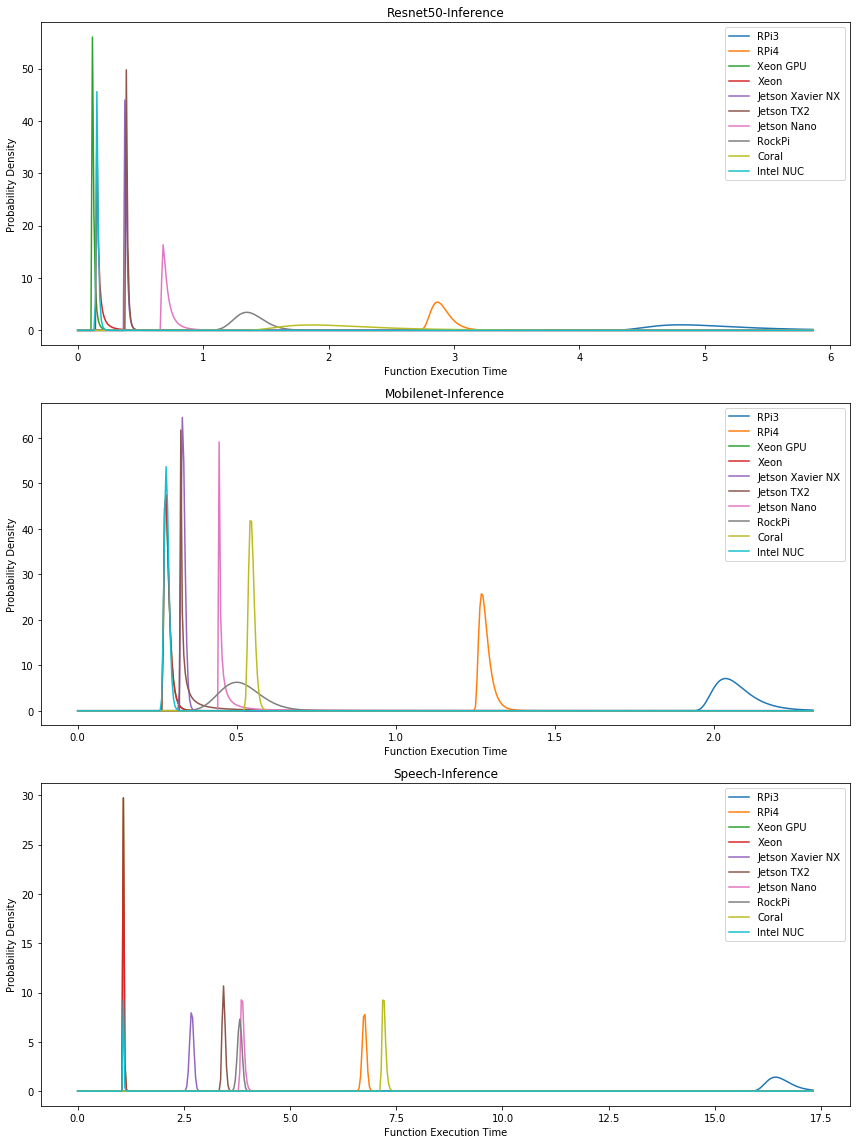
\includegraphics[width=\linewidth]{graphics/graphs/devices_fets.png}
%DIFDELCMD <     %%%
%DIFDELCMD < \caption{%
{%DIFAUXCMD
\DIFdelFL{Probability density functions of the \mbox{%DIFAUXCMD
\glspl{fet} }\hskip0pt%DIFAUXCMD
of the different devices we simulate}}
    %DIFAUXCMD
%DIFDELCMD < \label{fig:devices_fets}
%DIFDELCMD < \end{figure}
%DIFDELCMD < 

%DIFDELCMD < %%%
\DIFdel{Figure \ref{fig:devices_fets}
shows the \mbox{%DIFAUXCMD
\gls{fet} }\hskip0pt%DIFAUXCMD
distributions for these functions on the hardware outlined in Table \ref{tab:ether_devices}.
}%DIFDELCMD < 

%DIFDELCMD < %%%
\DIFdel{Because FaaS-Sim originally only supported response time evaluations due to \mbox{%DIFAUXCMD
\gls{fet}}\hskip0pt%DIFAUXCMD
, we extend it to also include the network time incurred from request transfers.
To enable this functionality, we introduce the notion of clients explicitly.
They are represented via nodes in the underlying network topology, just like the serverless cluster's nodes are.
Each request is dispatched from a client, sent to the nearest running load balancer instance, on to the function instance the load balancer selects, and back the same way.
}%DIFDELCMD < 

%DIFDELCMD < %%%
\DIFdel{The load pattern clients exhibit in FaaS-Sim can be fully controlled.
Generally, clients follow a predefined request pattern, either individually or globally, but absolutely any pattern required can be implemented.
This allows the simulation of differently active clients, differently active regions, and request patterns that change depending on system parameters.
}%DIFDELCMD < 

%DIFDELCMD < %%%
\DIFdel{To extract data for later analysis, FaaS-Sim features fine-grained and extensible trace-logging of all requests and system events.
}\section{\DIFdel{Network Simulation and Topologies}}
%DIFAUXCMD
\addtocounter{section}{-1}%DIFAUXCMD
\DIFdel{Because this work places a particular emphasis on network optimization, the network simulation component of FaaS-Sim is of particular relevancy to us.
Under the hood, FaaS-Sim relies on Ether\mbox{%DIFAUXCMD
\cite{rausch-ether} }\hskip0pt%DIFAUXCMD
for its networking.
}%DIFDELCMD < 

%DIFDELCMD < %%%
\DIFdel{Aside from vast option for customization, Ether supports a number of networking primitives that allow us to easily create a range of topologies.
In Ether's model, resources are usually, but not necessarily, grouped together in a cell.
The most important ones for our case are the }\textit{\DIFdel{LAN Cell}} %DIFAUXCMD
\DIFdel{and the }\textit{\DIFdel{Shared Link Cell}}%DIFAUXCMD
\DIFdel{.
The LAN Cell represents a set of compute nodes which are interconnected with each other in the way a LAN typically is, which means bandwidth is high, latency low, and variance small.}%DIFDELCMD < \\
%DIFDELCMD < %%%
\DIFdel{Contrary to that Shared Link Cells are more typical of what we might expect in an IoT scenario. 
It represents multiple nodes, which, as the name suggests, share a network connection between them.
This can, for example, be used to represent a number of edge devices which are grouped together into a small compute box and share a mobile internet connection for wider connectivity.
}%DIFDELCMD < 

%DIFDELCMD < %%%
\DIFdel{The networking simulation in Ether is based around the }\textit{\DIFdel{Link}} %DIFAUXCMD
\DIFdel{object\mbox{%DIFAUXCMD
\cite{rausch-ether}}\hskip0pt%DIFAUXCMD
, which represents a connection between nodes.
A mobile network connection, for example, would be considered a Link.
As Links represent connections, they also have a set bandwidth and latency.
To more accurately simulate how networks behave in real life, the latency of a link is not defined as a fixed number, but as a random distribution which gets sampled during simulation.
}%DIFDELCMD < 

%DIFDELCMD < %%%
%DIF <  decided to do a textual representation, as it was more useful
%DIF <  this is just a placeholder in case I change my mind
%DIFDELCMD < 

%DIFDELCMD < %%%
\DIFdel{To simulate network transfers Ether uses a flow-based simulation.
The transfer of a request from one node to another is considered a flow.
For each flow two steps are simulated: TCP connection establishment, and data transfer.
TCP connection establishment is assumed to be equal to $ 3 \cdot \text{latency}$ of the route the flow takes, based on the three-way SYN, SYN-ACK, ACK handshake of the TCP protocol.}%DIFDELCMD < \\
%DIFDELCMD < %%%
\DIFdel{The data transfer is where the flow simulation component is used.
Each flow consists of a number of hops, connected by links.
Each of these links has a set latency, bandwidth, and potentially a number of other flows currently being transferred.
To calculate how long data transfer takes, we first determine the bandwidth.
The bandwidth is determined by the minimum bandwidth available from any of the flow's links.
What exactly this is depends on the general bandwidth of the link in question, and by how many flows have to share this available bandwidth.
Once the bandwidth of the flow is determined we can simply calculate how long data transfer will take, given a request of known size.
To preserve the impact different flows have on each other, once a flow is added to the system, or once a flow is completed and thus removed, every link of the flow is updated and potentially recalculates the bandwidth of other running flows.
Other flows might be unaffected, but may also see and increase or decrease in available bandwidth depending on whether there are now more or fewer flows competing.
If flows are competing for bandwidth, they are all treated with equal priority, and share equally in the available bandwidth.
}%DIFDELCMD < 

%DIFDELCMD < %%%
\DIFdel{The topologies we use for our evaluations are based on the concept of smart cities\mbox{%DIFAUXCMD
\cite{suSmartCityApplications2011}}\hskip0pt%DIFAUXCMD
.
In this context we assume there may or may not be a central point in the city which provides a high amount of computational capability, i.e. a data center, and that the majority of computational capability will be interspersed throughout the city alongside with the clients.
}%DIFDELCMD < 

%DIFDELCMD < %%%
\DIFdel{For these edge-located resources we assume that two major types exist: }\textit{\DIFdel{Smart Poles}} %DIFAUXCMD
\DIFdel{and }\textit{\DIFdel{\mbox{%DIFAUXCMD
\gls{ran} }\hskip0pt%DIFAUXCMD
Towers}}%DIFAUXCMD
\DIFdel{.
We consider \mbox{%DIFAUXCMD
\gls{ran} }\hskip0pt%DIFAUXCMD
Towers to be any type of LTE or 5G mobile base station, which in our smart city scenario would additionally be equipped with edge computing capability.
The Smart Poles we consider to be a functionally similar, though comparatively smaller device, much like the Huawei PoleStar\mbox{%DIFAUXCMD
\cite{huaweiPolestar}}\hskip0pt%DIFAUXCMD
, which is also equipped with computational capability, albeit less of it, and providing a connection to the wider network.
We assume that these Smart Poles would be spread out throughout the city like sensor nodes in the Array of Things\mbox{%DIFAUXCMD
\cite{catlettArrayThingsScientific2017a}}\hskip0pt%DIFAUXCMD
, a real world edge computing and smart city sensing deployment.
In terms of latency and bandwidth we assume latency to Smart Pole devices to be in the same ballpark as WiFi connections, while \mbox{%DIFAUXCMD
\gls{ran} }\hskip0pt%DIFAUXCMD
Tower connections are in line with what one would typically expect of LTE or 5G connections respectively.
In keeping with our methodology of informing simulation values with real world measurements where possible, we used the research conducted by Braud et al.\mbox{%DIFAUXCMD
\cite{braudMulticarrierMeasurementStudy2019} }\hskip0pt%DIFAUXCMD
and Nikravesh et al.\mbox{%DIFAUXCMD
\cite{nikraveshMobileNetworkPerformance2014a} }\hskip0pt%DIFAUXCMD
on real world LTE network characteristics to inform our parametrization of these connections.
We also assume that truly low latency connections for client devices are only provided by physically near access points such as the aforementioned Smart Pole devices, as research on wireless network technology indicates that there is a fundamental tradeoff between bandwidth, latency, and reliability\mbox{%DIFAUXCMD
\cite{soretFundamentalTradeoffsReliability2014}}\hskip0pt%DIFAUXCMD
.
}%DIFDELCMD < 

%DIFDELCMD < \begin{figure}
%DIFDELCMD <     \centering
%DIFDELCMD <     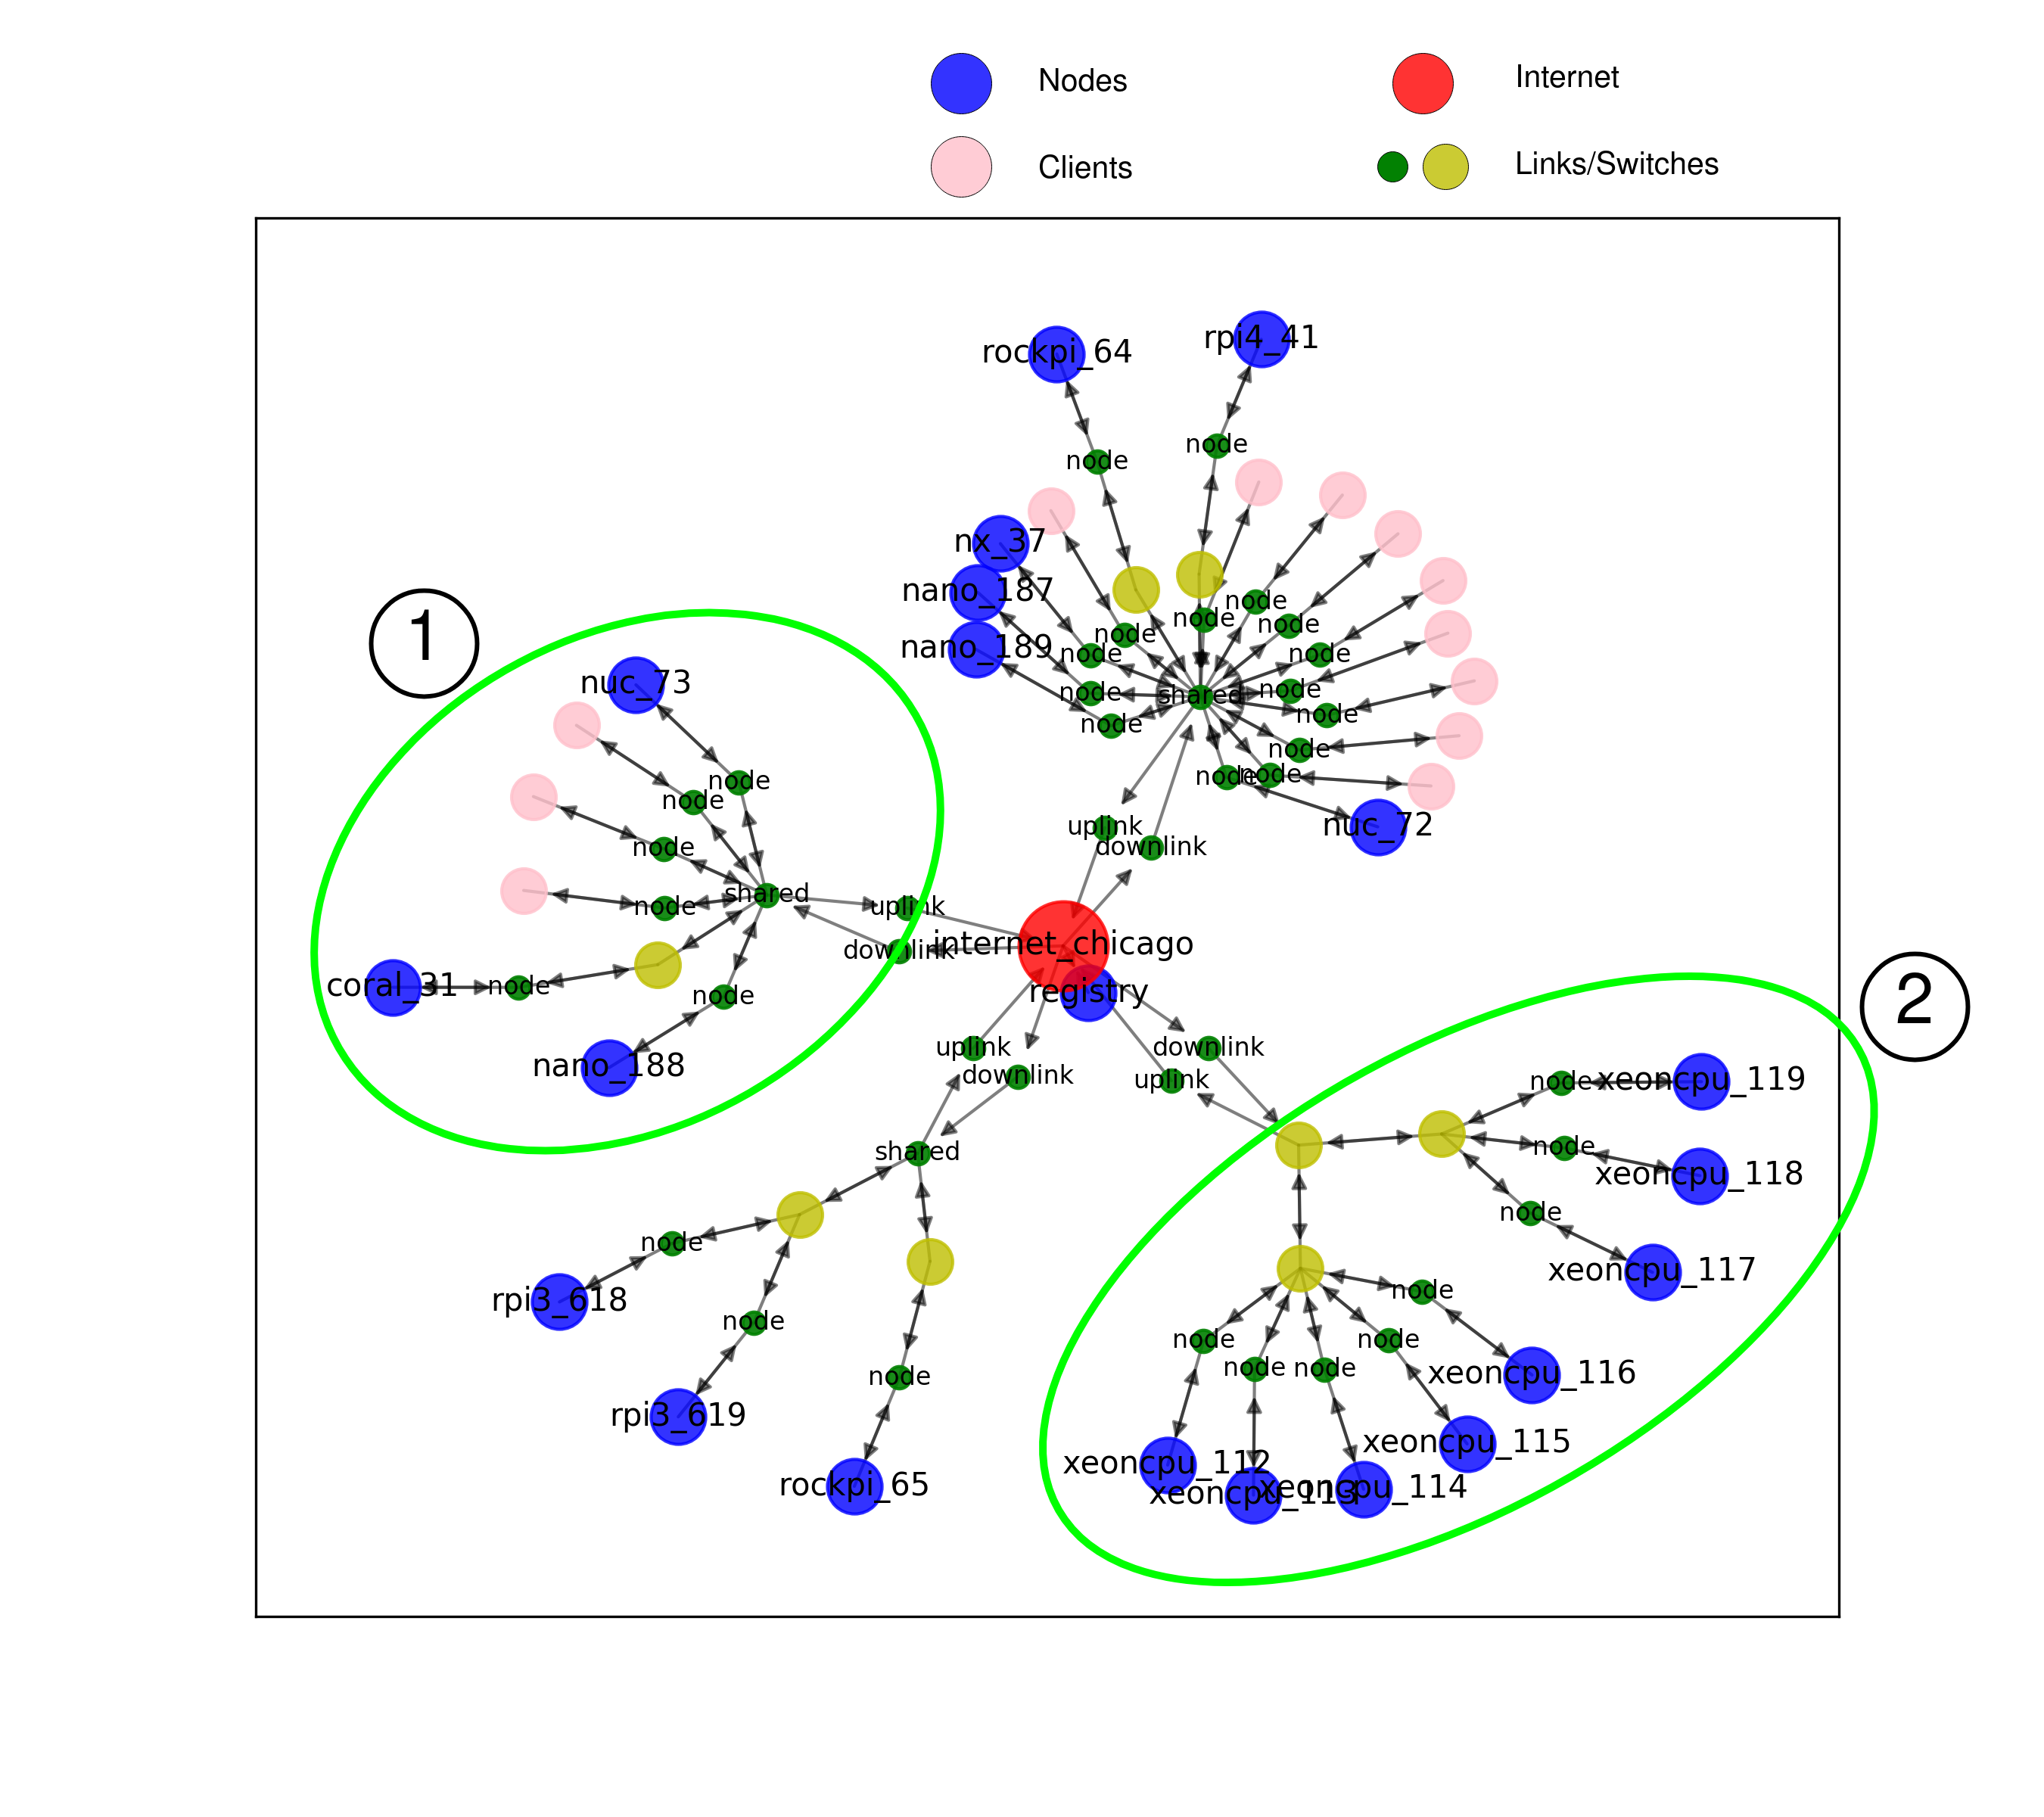
\includegraphics[width=\linewidth]{graphics/diagrams/tiny_topo.png}
%DIFDELCMD <     %%%
%DIFDELCMD < \caption{%
{%DIFAUXCMD
\DIFdelFL{Simplified network topology of a single smart city. Centered around the internet backbone uplink (red), 1) shows edge devices co-located with client devices. 2) shows a small cloud data center or cloudlet. Note the lack of clients directly connected to the cloudlet.}}
    %DIFAUXCMD
%DIFDELCMD < \label{fig:tiny_topo}
%DIFDELCMD < \end{figure}
%DIFDELCMD < 

%DIFDELCMD < %%%
\DIFdel{Finally, Figure \ref{fig:tiny_topo} shows a simplified visualization of how one of our smart city topologies is structured.
Note that latency cannot be read from this visualization and that distances between nodes on the visualization do not correspond to network distances whatsoever.
The wider internet, presented as a red circle, is how communication to areas not deemed within the city, or general web-services such as container registries would be routed.
Also note that we only represent logical network links and connections in our topologies, which means that while in truth there might be tens of network hops between an edge node and the wider internet (e.g. through the nearest backbone uplink), for simulation performance reasons we do not include these in our model.
%DIF <  1 page
}\section{\DIFdel{Using Empirical Data in Simulations}}
%DIFAUXCMD
\addtocounter{section}{-1}%DIFAUXCMD
\DIFdel{As already described FaaS-Sim\mbox{%DIFAUXCMD
\cite{faas-sim-github}}\hskip0pt%DIFAUXCMD
, the serverless simulator we use, is a trace-driven simulator\mbox{%DIFAUXCMD
\cite{thomas-thesis}}\hskip0pt%DIFAUXCMD
, meaning that it relies on measurements of real world data to make its results more representative.
The types of empirical data that can be used to improve simulation accuracy are very broad, but are typically limited to those that actually affect the metrics one is interested in measuring.
Usually this includes the memory consumption, CPU utilization, network utilization and storage size of different software components present in the system.
It can, however, also include more specific metrics such as deployment, staring, stopping and teardown times of container in a Kubernetes cluster\mbox{%DIFAUXCMD
\cite{skippy}}\hskip0pt%DIFAUXCMD
.
}%DIFDELCMD < 

%DIFDELCMD < %%%
\DIFdel{Similar to how Raith et al. extended FaaS-Sim to include traces of real function executions to better represent \mbox{%DIFAUXCMD
\glspl{fet} }\hskip0pt%DIFAUXCMD
\mbox{%DIFAUXCMD
\cite{philipp-da}}\hskip0pt%DIFAUXCMD
, we perform experiments to inform how load balancers are modelled within the system.
Since in current serverless frameworks ingress-points, which is equivalent to a load balancer in our case, are considered as just another service, they compete with function replicas for resources.
As a result the resource usage of typical application level load balancers is an important metric for us to capture and integrate into the serverless simulator.
}%DIFDELCMD < 

%DIFDELCMD < %%%
\DIFdel{For our empirical evaluations we use a real Kubernetes cluster that features a variety of heterogeneous nodes.
Since we deal with edge computing applications, and resource heterogeneity is a core challenge of edge computing\mbox{%DIFAUXCMD
\cite{shiEdgeComputingVisionChallenges2016}}\hskip0pt%DIFAUXCMD
, having a range of different nodes to evaluate performance on is critical to account for variance incurred by the use of different types of devices.
We also make use of and extend galileo\mbox{%DIFAUXCMD
\cite{galileo-github}}\hskip0pt%DIFAUXCMD
\mbox{%DIFAUXCMD
\cite{operating-energy-aware-galileo}}\hskip0pt%DIFAUXCMD
, a framework built for distributed load testing, as it allows us to easily define request patterns and loads that then get executed.
By using this we can go beyond measurements of baseline resource consumption and examine the relationship between the request load of a service and its performance and resource consumption profile.
To gather performance data of individual containers in a Kubernetes cluster, galileo relies on and integrates with telemd\mbox{%DIFAUXCMD
\cite{telemd-github}}\hskip0pt%DIFAUXCMD
.
Telemd is a daemon application that can gather a number of system metrics at specified intervals, including CPU utilization, memory consumption, disk I/O, and network transfers.
}%DIFDELCMD < 

%DIFDELCMD < %%%
%DIF <  what do I actually want to say?
%DIF <  empirical experiments important to inform real world data
%DIF <  need to be aligned with the hardware simulated e.g. arm devices, x86, etc. etc.
%DIF <  this needs to be measured somehow -> galileo
%DIF < 
%DIF < 
%DIF <  1-2 pages
\section{\DIFdel{Captured Metrics}}
%DIFAUXCMD
\addtocounter{section}{-1}%DIFAUXCMD
\DIFdel{There is a significant number of metrics that could be captured using such a simulation. With FaaS-Sim we capture traces of the requests being sent, and major system events.
The major system events are the addition or removal of deployments, as well as all scaling and scheduling decisions with respect to functions and load balancers.
For requests our traces provide the following information: \mbox{%DIFAUXCMD
\gls{trt}}\hskip0pt%DIFAUXCMD
, \mbox{%DIFAUXCMD
\gls{fet}}\hskip0pt%DIFAUXCMD
, waiting time, request client, load balancer instance, function instance, and the network times between client, load balancer and function instance.
The waiting time refers to the elapsed between a request having been received by a function instance, and the request being processed.
Waiting times occur if a node receives requests faster than it can process them.
In terms of resource usage, the resources reserved by the simulated Kubernetes pods, which correspond to the requirements defined in Kubernetes deployment manifests, are also recorded.
Note that this does not necessarily correspond to actual resource usage.
Because these reserved resource metrics are used for Kubernetes' scheduling decisions, we believe they are still worth being captured.
}%DIFDELCMD < 

%DIFDELCMD < %%%
\DIFdel{In keeping with the set of potential metrics outlined by Aslanpour, Gill and Toosi\mbox{%DIFAUXCMD
\cite{aslanpourPerformanceEvaluationMetrics2020a}}\hskip0pt%DIFAUXCMD
, we pay particular attention to response times, potential \mbox{%DIFAUXCMD
\gls{sla} }\hskip0pt%DIFAUXCMD
levels and oscillation mitigation.
We also introduce more qualitative metrics, related to our particular evaluation scenario, such as the share of requests being routed outside of the city or network region they originate in.
}\DIFdelend % Target: 20ish pages total; 13 pages of text, 7 pages of images
\chapter{Load Balancers and Their Placement}
In this chapter we describe our chosen approach for improving the performance of network bound workloads in serverless edge computing environments. We start by explaining our considerations when developing our approach in the context of a serverless edge computing system, and showing in what way our solution changes the system. From there we go into detail about how the load balancing mechanism of our solution works, how it is different from the currently employed methods, and how the choices made in regard to the load balancing method inform other parts of the proposed approach.
Lastly we go into our approach to scaling and scheduling load balancers among the nodes present in the serverless edge computing system. We make use of osmotic scaling and scheduling, a method previously outlined in existing literature. Using this idea of osmotic scaling and scheduling, we provide a concrete implementation of such an approach for placing and deciding on the number of load balancers in the system. The implementation is designed with current state of the art systems such as Kubernetes as the basis, and can thus be used as a reference implementation for use outside of a simulation context. The approach also addresses the challenges of edge computing environments that make current approaches, developed with the cloud in mind, unsuitable. Specifically our approach addresses issues of location awareness, device and network heterogeneity, and dynamically changing workload conditions.
% Target: 2ish pages \w graphics
\section{Concept}
% Note: mention that in our context load balancing and entry-gateway are sort of equivalent. Show their relation a bit
% Note: Mention that our approach uses the method of using real-life experiments to inform simulation

To understand the approach we first take a step back to view the boarder technical context the solution addresses and is built around.
As previously outlined, our solution aims to improve the performance of network bound workloads.
In the context of serverless edge computing systems network bound workloads are characterized by the network being the main or a significant contributing factor to the overall response time.
\begin{figure}
    \centering
    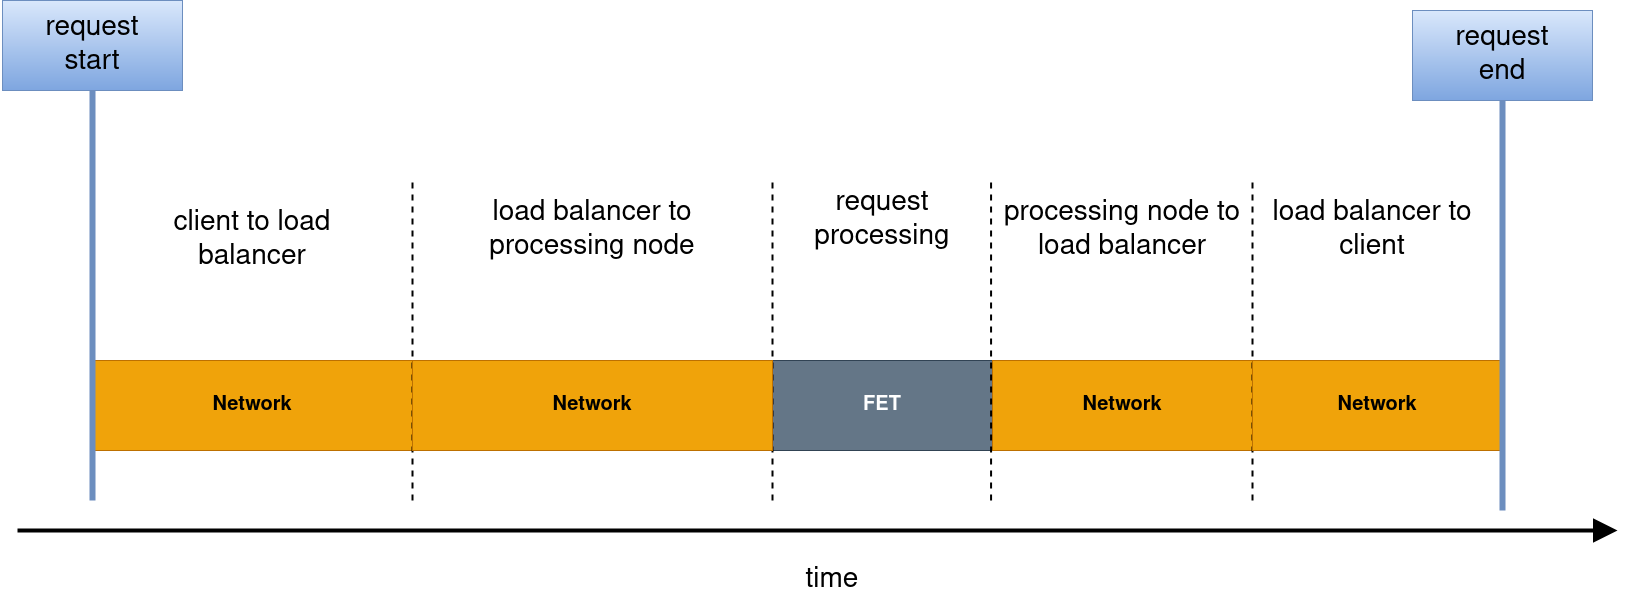
\includegraphics[width=14cm]{graphics/diagrams/request_overview.png}
    \caption{A generic view of the different parts that make up the total request processing time from the perspective of our approach}
    \label{fig:request_net_fet_overview}
\end{figure}
In Figure \ref{fig:request_net_fet_overview} we can see the different processing steps we consider for a request.
A network bound workload in this sense is one where the time taken up by the network portion of handling the request is proportionally speaking significantly larger than the portion taken by the \gls{fet}.
This is typically the case because either the request contains a lot of data that needs to be transported, or because the \gls{fet} is very short.

The primary way by which our approach improves the response times of network bound workloads is thus by reducing the amount of time spent on the network transfer portion of handling a client request.
While optimizing \glspl{fet} is not the primary objective of our approach, at least from a systems design perspective, it still has the potential to additionally reduce \glspl{fet} compared to current methods.
We consider the structure and makeup of the serverless computing system to be a given factor. As a result our approach aims to reduce network times not by changing the network makeup itself, but by utilizing the existing resources as effectively as possible. From a network-optimization perspective this means that each request should take an optimal path from  the client to the node where the request is ultimately processed. 

\begin{figure}
    \centering
    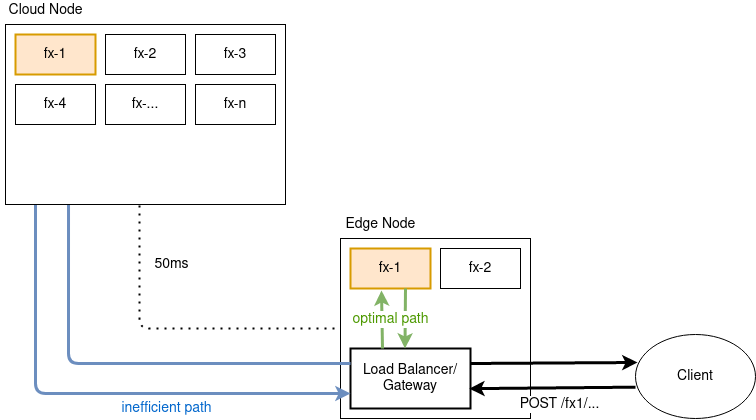
\includegraphics[width=12cm]{graphics/diagrams/efficient_path_example.png}
    \caption{Example diagram showing efficient and inefficient request routing based on network delay. "fx-1" through "fx-2" denote different types of function, and the dotted line denotes a network link between the cloud and edge node with a latency of 50ms}
    \label{fig:efficient_path}
\end{figure}

As can be understood quite intuitively in Figure \ref{fig:efficient_path}, round robin load balancing will in many cases lead to clearly suboptimal choices in terms of incurred network delay. The figure also shows the three key components we consider when trying to make network location based decisions: The client, the load balancer, and the node. Because our approach solely considers application level load balancers, since serverless platforms typically require these for their advanced routing decisions, any given request takes a path from the client to the load balancer, then to the selected upstream node, and back the same way.

Subsequently we want to incur the minimal amount of delay possible from both the hop between the client and load balancer, as well as between the load balancer and upstream node. Our proposed approach handles these two kinds of hops separately, at least for the most part. Since the scope of this work does not include optimizing the location of the serverless function instances themselves, this means we can improve performance through the following methods:
\begin{enumerate}
    \item \textbf{Intelligent load balancing decisions:} load balancers should choose upstream nodes that are both close in the network, and have \glspl{fet} short enough as not to negate the performance won through network proximity
    \item \textbf{Effective placement of load balancers:} the scheduler of the serverless system should place load balancers at locations in the network where they are in close proximity to clients and serverless function instances requested by these clients
    \item \textbf{Efficient scaling of load balancers:} the amount of load balancers should be high enough to provide the needed performance improvement, but not so high that the resources consumed by the load balancers diminish or even negate that effect
\end{enumerate}
In our approach the first method is provided by the load balancer itself. It is continuously updated with information where function instances, typically also referred to as \textit{replicas}, are located. Based on this and other information gathered by the load balancer, it tries to make decisions that lead to faster overall request responsiveness by selecting upstreams that are close and provide fast \glspl{fet}.

The other two methods are handled by the osmotic joint scaling and scheduling component of our approach. While the different methods of improvement are split between these two components of our proposed solution, this does not mean that they are completely separate from each other. Naturally the scheduling and scaling decisions will influence the way in which the placed load balancers work, while these in-turn affect the data gathered for and available to the scaling and scheduling component. The specifics of these two components will be discussed in the next two sections. 

It is also important to note that a significant amount of the approaches' implementation details are not chosen arbitrarily, but are rather the result of continuous cycle of experimentation and evaluation. While not detailed in the approach, the evaluation, result, and discussion chapters of this thesis include some of these experiments, in particular those that give additional insight into the problem domain and yielded results useful beyond informing this specific approach.
% Target: 8 pages with figures
\section{Least Response Time Load Balancing}
In this section we describe the role the load balancer plays in the context of our approach, how it is related to the underlying serverless platform, and the details of how it is implemented.

\subsection{Load Balancing Concepts}
While load balancing might at first appear as a rather simple problem, venturing outside cloud-centric scenarios, where resource homogeneity can be assumed, makes it much more complex of a challenge.
Since we feel the changes implied by resource heterogeneity are often only implicitly covered in literature, or an understanding of the problem is assumed, we believe that it is beneficial to describe it in more detail. This not only helps form a basis on which subsequent research can build, but also gives a lot of contextual information on how our approach relates to the underlying formal problem.

For our formulation of the load balancing problem we consider two types of resources: nodes, and network links. Nodes are the compute nodes in the cluster, and are characterized by the compute capabilities they possess and the function instances they host. Network links are characterized by their latency, and their bandwidth.
\begin{figure}
    \centering
    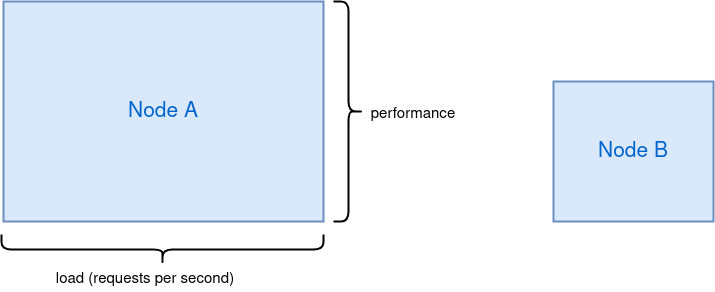
\includegraphics[width=12cm]{graphics/diagrams/load_balancer_squares.png}
    \caption{Rectangles representing a resource in our problem visualization}
    \label{fig:lb_squares_basic}
\end{figure}
To get a more intuitive understanding of the problem we developed a visualization, where resources are depicted as rectangles, where their dimensions correspond to their characterizing attributes. Figure \ref{fig:lb_squares_basic} shows an example of this. The width of the rectangle corresponds to the \textit{load} of the system, in our case measured in \gls{rps}, and the height corresponds to the performance, which since we are concerned about response times is the response time in milliseconds. One should note that, even though maybe counter intuitive, a greater height corresponds to higher performance, which in turn means \textit{lower} response times.
A core concept of this visualization is the capability of resources to \textit{stretch} or \textit{compress}. This means increasing or decreasing width or height of the resource, while doing the inverse to the other side. The condition is that the total area of the resource, i.e. the product of width and height, must be consistent throughout this process. This is effectively the way in which performance regression is modeled in this visualization, but one should not that this way only works under the condition that performance regression is linear with respect to the load. Luckily this is close to observed real world behaviour, %todo cite this
meaning that at least for understanding the underlying problem this visualization holds.
There are, however, limits to this stretching or compressing resources. From a visual perspective there is a bounding box around each resource, which cannot be exceeded in either height or width. This corresponds to the real world behaviour of workloads not getting faster beyond a certain point, even if resources would be available one one side, and requests simply timing out once responses exceed a certain time limit.
\begin{figure}
    \centering
    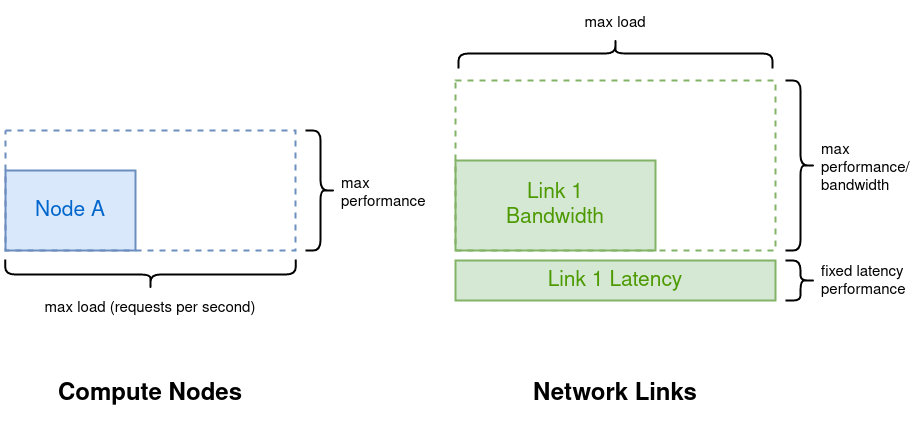
\includegraphics[width=14cm]{graphics/diagrams/lb_squares_real.png}
    \caption{Rectangles representing Node and Network Link resources, including their respective bounding boxes showing maximum load and performance capabilities}
    \label{fig:lb_squares_real}
\end{figure}
Network link resources work slightly differently, as they have a fixed component, dictated by the latency of the link, and a variable component set by the bandwidth. The variable component works as just described, while the static component is constant. Figure \ref{fig:lb_squares_real} shows the variable and static components along with their limits.

Resources can be conditionally linked. This maps the real world conditions of nodes being attached to the cluster via network links. Just like in actual clusters multiple nodes can be dependent on the same network link, and network links in turn can depend on another network link. 

\begin{figure}
    \centering
    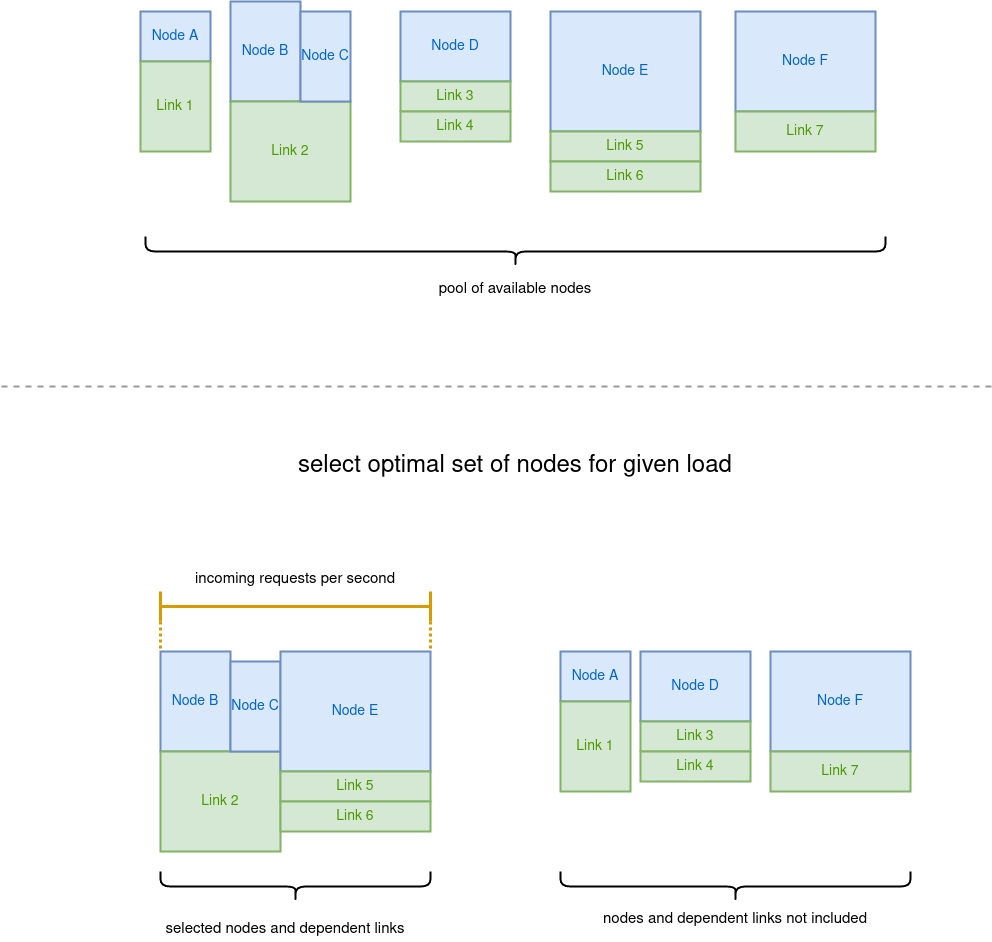
\includegraphics[width=14cm]{graphics/diagrams/lb_optimal_selection.png}
    \caption{Example visualization of an optimal selection of nodes, including their network links, for a given request load. Bounding boxes showing min/max load/performance, and fixed network latency performance parts are not displayed to keep the example simple.}
    \label{fig:lb_optimal_load}
\end{figure}

With this definition we can define the optimization problem an effective edge load balancer is trying to solve. The input to this problem is the given request load arriving from clients. In our visualization his corresponds to a set width. The objective is then to select nodes which when combined have the same width as the incoming client node, while at the same time maximizing the area of the nodes and network links selected. One needs to keep in mind that network links are not selected directly, but are implicitly included if selected nodes depend on them. Figure \ref{fig:lb_optimal_load} shows an example of such an optimal selection.

If the area is maximized in this optimization problem, response time is minimized, which is the goal a load balancer is trying to achieve.


While this visualization and problem is still relatively straightforward, there are other significant factors that we omitted until now:
\begin{enumerate}
    \item There are multiple functions, meaning that there are multiple "widths" or bins that need to be filled
    \item Functions share compute capabilities of nodes, meaning that performance regression, i.e. stretching and compression, needs to be considered over all functions running on a node
    \item Dependencies between network links and nodes aren't necessarily known
    \item Some network links necessarily handle traffic from outside the system, making performance regression assessment harder
    \item Actual performance profiles, i.e. dimensions, of nodes and functions aren't known
    \item Performance profiles, capabilities, client load, and function deployments change dynamically over time
\end{enumerate}

Considering these factors, load balancing in this context is a much higher-dimensional and thus more complex problem, where it is intuitively not clear whether an optimal solution is possible or if explicitly pursuing it in practise is even computationally feasible.


Since the true performance and regression characteristics of the nodes and network links are unknown, a load balancing solution needs to consider how this lack of information can be addressed. 
The simplest way to gather this information is by sending requests to nodes and observing response times. While this can yield insight into performance characteristics, these observations are merely a statistical sample, making them at least somewhat prone to misinterpretation. Especially when it comes to more complex behaviours such as functions sharing compute resources of nodes, or multiple nodes sharing network links.

Depending on the goals of the load balancer there is a risk/reward dynamic at play when it comes to sending requests to nodes in order to learn more about their performance characteristics. On one hand this can lead to "discovering" nodes that offer high performance and are able to handle a large number of requests, but on the other hand it could also lead to poor performance for those very requests in case network or compute capabilities are sub par.
There is no single correct answer to this dilemma, since the efficacy of any given solution would depend on the specific goals and tolerances of the application in question. In case \glspl{sla} exist that stipulate a certain response time for a minimum percentage of requests the risks might outweigh potential rewards, while an application that is somewhat tolerant to a fraction of requests being slow might experience a great performance uplift overall.
For our approach we consider \glspl{sla} to be out of scope, and therefore do not further address ways to address them. At the same time we want to point out that these are potentially relevant aspects for bringing serverless edge computing towards production readiness in the industry, and therefore highlight the areas where further study is needed.

\begin{figure}
    \centering
    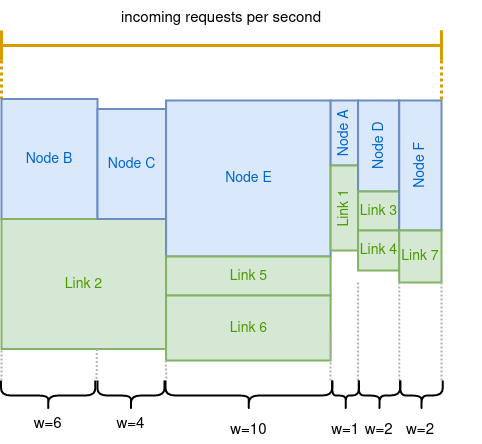
\includegraphics[width=10cm]{graphics/diagrams/lb_weights.png}
    \caption{Our approach as seen through the described visualization. All nodes are included in the "solution", and their load is determined by the load balancer assigning weights}
    \label{fig:lb_weights}
\end{figure}

Considering the myriad of potentially complicating factors for load balancing, in particular if one were to attempt to directly model the problem algorithmically, we decided to take a comparatively simple approach for our load balancing method.
In our approach we base our load balancing decisions solely on the total response time as it is observed by the load balancer. This means that we do not differentiate between times incurred from \gls{fet} and the times incurred from the networking portion. In this way we treat the total response time as a \textit{black box metric} to the overall system.
Our approach is to always include every single node in the "solution" to selecting appropriate nodes for the given width. This means that over the long term our approach gathers information about every potential node for every function replica that gets requested.
The disadvantage of this approach is that it dispatches requests to nodes that would not be included in a mathematically optimal solution, meaning that is will never reach the optimal performance possible assuming perfect knowledge of the system.
To counteract the performance penalty of including all nodes in the solution we assign them weights based on the response time they achieve.
This allows the load balancer to strike a balance between gathering information about the performance of the nodes available to the cluster, and processing requests as fast as possible.
Figure \ref{fig:lb_weights} shows the view of our approach on the system as described in the visualization. Note that the networking portion is not present, as our approach only considers the total response time in relation to the node it was sent to. Our approach also views each function replica separately, meaning that joint performance degradation of co-located function replicas is not modeled explicitly, only implicitly via the degraded performance observable through total request response times on that node.

There are a number of important considerations about the practical realization of our approach, which we will discussed next.


\subsection{Implementation}
As was just outlined our approach uses the response time as a black box metric to get insights into the system, and thus make load balanced decisions based on that information.
Since this basic idea does not constitute a concrete and testable approach we need to define the implementation details.

A well-known and simple implementation of this idea is the \textit{least response time} method of load balancing.
In this approach the server with the lowest average response time gets chosen whenever a request needs to be processed.
While this certainly works in general there are a few issues with this approach when it comes to serverless edge computing.
First, this approach can be problematic when it comes to co-located functions, as the load is not distributed among upstreams equally.
This leads to the fastest node being selected until its performance degrades enough for the next best node to be chosen.
Since there is no coordination that ensures some kind of balance, other functions that happen to be deployed on that node could experience severely hampered performance unexpectedly.
Second, this method does not take into account that the performance of nodes is, at least at first, unknown, and that it can change. A node that generally performs exceptionally well could be permanently excluded if at one point, for a spurious reason, performance was poor. A naive least response time load balancer would then likely rotate between a small handful of nodes that at one point performed well, effectively ignoring potentially better solutions.
These reasons point to the need of a more sophisticated approach than a naive implementation of least response time load balancing.

\subsubsection{Metrics Collection}
As explained, in our approach the metric used for load balancing decisions is the response time, specifically the time it takes between the load balancer forwarding the request to the selected upstream, and the load balancer receiving the response to the request.

Based on the response time data there are a number of performance metrics that could be calculated. Since our goal is to reduce the average total response time, we also chose the average response time as the key metric for load balancing decisions.
Depending on the requirements the load balancer needs to fulfill, other metrics could be used. A load balancer that is supposed to ensure a type of \gls{sla} might, for example, benefit from a percentile based metric instead.

In addition to effectively summarizing the performance of nodes, the metric needs to be time sensitive. Considering the performance of nodes can change over time, more recent values are more important as an indication of performance than those that lie farther back.
To address this, our approach makes use of a moving average with fixed window size.
We chose to use an exponential moving average since it has a number of advantages over more typical implementations.

\DIFdelbegin \[\DIFdel{\text{Given the previous average value } \mathbf{\bar{r}_{0}}\text{, the most recent response time } \mathbf{r}{,}}\]%DIFAUXCMD
\[\DIFdel{\text{the time passed since the last request }\mathbf{\Delta t} \text{, and the window size }\mathbf{w}}\]%DIFAUXCMD
\[\DIFdel{\text{The new average value }\mathbf{\bar{r}_{1}} \text{ is}}\]%DIFAUXCMD
\DIFdelend \DIFaddbegin \DIFadd{Given the previous average value $\mathbf{\bar{r}_{0}}$, the most recent response time $\mathbf{r}$, the time passed since the last request $\mathbf{\Delta t}$, and the windows size $\mathbf{w}$, the new average value $\mathbf{\bar{r}_{1}}$ is
}

\DIFaddend \[\bar{r}_{1} = (1 - e^{\frac{-\Delta t}{w}}) \cdot r + e^{\frac{-\Delta t}{w}} \cdot \bar{r}_{0}\]

The most significant advantage of this implementation over ones that use a buffer or a similar data structure, is precisely that complex data structures are not required. For each upstream only two values need to be recorded:
\begin{enumerate}
    \item The time the moving average was last updated
    \item The current value of the moving average itself
\end{enumerate}
While there are situations, where this can be less accurate, it is far easier to implement than buffer based solutions, since with these the required buffer size is unknown thus leading to frequent memory allocations and de-allocations.
Using an exponential moving average ensures minimal memory consumption, while at the same time being easy to understand and implement.

\subsubsection{Choosing Upstreams}
With the metrics collected what remains is deciding on upstreams based on those values. As previously outlined, naively choosing the upstream with the lowest average response time is potentially problematic.
For this reason our approach uses weighted round robin to decide which upstream should service a given request, where the response time metrics determine the weight assigned to each upstream.

The decision how exactly this weighted round robin gets implemented is surprisingly important, since the load balancing decisions affect the accuracy and volume of performance data gathered on each node, thus creating a feedback cycle that can, depending on the situation, lead to sub optimal performance.
For our approach we decided to use the same method employed by NGINX\cite{nginx}, a popular web-server and request proxy.
We chose this approach after experimenting with other solutions, and analyzing their performance profiles and characteristics with regard to the unique challenges posed by serverless edge computing environments.
Compared to other approaches is has the advantage of being deterministic, leading to all nodes being chosen eventually, which gives the load balancer sufficient data to make informed decisions, while at the same time distributing traffic in a mixed fashion between upstreams of different weights.
The evaluation methodology and experiment results of these experiments can be found alongside the general evaluation in the subsequent chapters.

\begin{algorithm}
  \KwIn{Set of available nodes $n_{0},n_{1},n_{...} \in N$}
  \KwIn{Weights for each of the nodes $w_{n_{0}}, w_{n_{1}}, ... \in W$}
  \KwIn{Current counter value for each node. $c_{n_{0}}, c_{n_{0}}, ... \in C$}
  \KwOut{The node the next request should go to}
    \For{$n \in N$}
    {
        $c_{n} \leftarrow c_{n} + w_{n}$ \Comment{add node weight to its counter}
    }
    $\text{selectedNode} \leftarrow n: c_{n} = max\{c: c \in C\}$ \Comment{select node with highest counter value}\\
    $c_{\text{selectedNode}} \leftarrow c_{\text{selectedNode}} - \sum_{w \in W}w$\\

  \Return{selectedNode}

  \caption{Smooth Weighted Round Robin}
  \label{alg:smooth-wrr}
\end{algorithm}
%todo: maybe rework this to be a bit more elegant
% currently a bit too much of a mashup between, math, set theory, code

\begin{table}[]
\centering
\begin{tabular}{llll}
Node          & \textbf{A}                & \textbf{B}                & \textbf{C}                \\
Weight        & \textbf{4}                & \textbf{2}                & \textbf{1}                \\ \hline
Iteration \#1 & \cellcolor[HTML]{FFCE93}4 & 2                         & 1                         \\
              & -3                        & 2                         & 1                         \\ \hline
Iteration \#2 & 1                         & \cellcolor[HTML]{FFCE93}4 & 2                         \\
              & 1                         & -3                        & 2                         \\ \hline
Iteration \#3 & \cellcolor[HTML]{FFCE93}5 & -1                        & 3                         \\
              & -2                        & -1                        & 3                         \\ \hline
Iteration \#4 & 2                         & 1                         & \cellcolor[HTML]{FFCE93}4 \\
              & 2                         & 1                         & -3                        \\ \hline
Iteration \#5 & \cellcolor[HTML]{FFCE93}6 & 3                         & -2                        \\
              & -1                        & 3                         & -2                        \\ \hline
Iteration \#6 & 3                         & \cellcolor[HTML]{FFCE93}5 & -1                        \\
              & 3                         & -2                        & -1                        \\ \hline
Iteration \#7 & \cellcolor[HTML]{FFCE93}7 & 0                         & 0                         \\
              & 0                         & 0                         & 0                        
\end{tabular}
\caption{An example of weighted round robin iteration results when using Algorithm \ref{alg:smooth-wrr} as we do in our approach. Colored cells indicate the selected node at the iteration.}
\label{tab:smooth-wrr-demo}
\end{table}

Algorithm \ref{alg:smooth-wrr} shows a pseudo-code implementation of our weighted round robin component using the approach also used in the NGINX source code \cite{nginx-wrr}.
Table \ref{tab:smooth-wrr-demo} shows how this implementation of weighted round robin distributes requests between upstreams of different weights. Note that the proportions between the weights are considered when choosing upstreams without using a fixed ordering based on weight, meaning that choices of upstreams with lower weights are interleaved between choices of upstreams with higher weights. %todo rewrite this. It's super unclear what is meant by this.

The only part of our load balancing approach that is not yet described is how the average response time recorded is mapped to the weight used by our weighted round robin implementation.
There are a number of ways in which values like this can get mapped to weights.
There is, unfortunately, no single correct answer since the lack of precise information on the state and performance of nodes and the network prevents us from reliably making globally optimal load balancing decisions.
There are two factors that determine how response times are mapped to weights:
\begin{enumerate}
    \item The weight range response times should be mapped to
    \item The function by which they are mapped to these weights
\end{enumerate}

In our approach we chose to use a fixed range of weights, since this makes sure every upstream is assigned at least a fixed fraction of traffic.
This guarantees that the response times of all upstreams are sampled eventually, preventing a situation where a significant change in the performance of an upstream goes unnoticed forever.
The weight of each upstream is determined by it's average response time in the last value and calculated using the following formula:
\DIFdelbegin \[ \DIFdel{\text{Let } \bar{r} \in R \text{ be the set of response time averages, and }}\]%DIFAUXCMD
\[ \DIFdel{w_{\text{min}} \text{ the minimum weight, } w_{\text{max}} \text{ the maximum weight, then}}\]%DIFAUXCMD
\[ \DIFdel{\text{the weight for each response time average } w(\bar{r})\text{ is defined as}}\]%DIFAUXCMD
\DIFdelend \DIFaddbegin 

\DIFadd{Let $\mathbf{\bar{r} \in R}$ be the set of response time averages, $\mathbf{w_{\text{min}}}$ the minimum weight, and $\mathbf{w_{\text{max}}}$ the maximum weight. Then the weight for each response time average $\mathbf{w(\bar{r})}$ is defined as
}

\DIFaddend \[ w(\bar{r}) = max\{w_{\text{min}}, \frac{w_{\text{max}}}{(\frac{\bar{r}}{min\{\bar{r}: \bar{r} \in R\}})^{s}}\} \]
\DIFdelbegin \[ \DIFdel{\text{where } s > 0\text{ is a chosen scaling factor }}\]%DIFAUXCMD
\DIFdelend 

\DIFaddbegin \DIFadd{where $\mathbf{s > 0}$ is a chosen scaling factor.
}

%DIF >  \[ \text{Let } \bar{r} \in R \text{ be the set of response time averages, and }\]
%DIF >  \[ w_{\text{min}} \text{ the minimum weight, } w_{\text{max}} \text{ the maximum weight, then}\]
%DIF >  \[ \text{the weight for each response time average } w(\bar{r})\text{ is defined as}\]

%DIF >  \[ \text{where } s > 0\text{ is a chosen scaling factor }\]

\DIFaddend The scaling factor determines how weights correlate to response time. A scaling factor of 1 means that there is a linear relationship between the average performance and the weight.
Figure \ref{fig:weight_mapping_example} shows the effect different scaling factors have on weight mappings in the weight range of 1-10. Both continuous and integer values are shown, since it depends on the weighted round robin implementation which of the two can be used.
Based on grid-search experiments we chose a weight range of 1-25, and a scaling factor of \DIFdelbegin \DIFdel{2. (//note to me: these experiments should be expanded a bit and values updated if necessary)}\DIFdelend \DIFaddbegin \DIFadd{2, although we stress that there is no one optimal parameter choice for all circumstances}\DIFaddend .
The experiments that determined this choice will be described in detail in subsequent chapters.

% idea: factor (i.e. deciding on linearity) depends on how strong the link between performance and capacity is. i.e. if strong performance means high capacity, we can assign super high relative weights. Is this even important? Since on paper overload etc. should eventually lead to a balance being achieved, no?
% idea: spread (i.e. size of weight range) depends on how dynamic the system is and how high we value information gain, since high spread -> more optimal in static condition. low spread -> discovers changes faster in dynamic conditions.

\begin{figure}
    \centering
    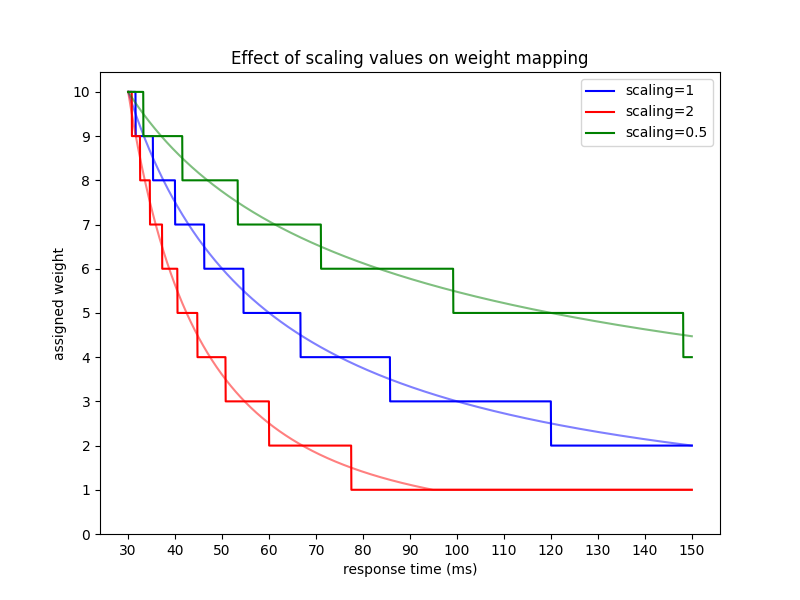
\includegraphics[width=10cm]{graphics/graphs/weight_mapping_scaling_example.png}
    \caption{Plot showing the effects of different scaling factors on how response time averages are mapped to weights.}
    \label{fig:weight_mapping_example}
\end{figure}


\subsubsection{Framework Integration}
In our approach the load balancers are assumed to be integrated into the serverless framework.
This means that load balancers are notified of changes to function replicas, meaning that they are always aware which functions exist, and which exact replicas are available for each function.
From a practical perspective this is simple to achieve in a production implementation as serverless frameworks already provide this information in some way, and the underlying technologies, typically some kind of container orchestration, also have means to retrieve the necessary data.

Apart from the available functions and their respective replicas, new load balancer instances are initialized with response time values and weights of already running load balancer instances nearby.
While the load balancer still needs to adapt its weights based on its specific client load and position in the network, this initial pre-loading of values allows it to converge on a stable configuration faster, thus resulting in quicker performance gains.


% Target: 8 pages with figures

% todo add dustar osmotic paper source!!! Osmotic Flow: Osmocitc Computing + IoT Workflow
\section{Osmotic Scaling and Scheduling}
In this section we describe our approach to scaling, and scheduling load balancer replicas, meaning the process by which we decide how many load balancer instances are in the system, and on which nodes they are placed.

\subsection{Osmotic scaler and scheduler}
To determine the number of replicas and their location we opted for an approach based on \textit{osmotic pressure}.
Like we outlined in previous chapters, osmotic pressure is a high level concept supposed to facilitate elastic diffusion, elastic diffusion being the process by which a central starting configuration, typically in the cloud, is extended to the edge dynamically based on request load with the goal of providing low latency communication for edge clients\cite{osmotic-middleware-rausch}. 
The general idea of this approach is that client requests generate pressure on nodes that are close to the clients, meaning that they could potentially host a load balancer instance, and then using this pressure in conjunction with a set threshold to determine both the number of load balancer instances and their locations.
If pressure at a node exceeds a certain level, because there are a lot of client requests originating close by, a load balancer will the, be placed at the node, thus lowering the pressure.
Conceptually this approach is supposed to create an equilibrium of pressure throughout the system, which results in a well-chosen set of load balancer instances.
This means that by using an osmotic approach, the scaling and scheduling decisions are effectively made together and cannot be controlled separately.

The main challenge of realizing an approach based on the concept of osmotic pressure is finding the method by which pressure is calculated. This can be particularly challenging when the system requires a manually set pressure threshold, since this requires the threshold value to fulfill a number of criteria:
\begin{enumerate}
    \item \textbf{Intuitive:} the threshold value should be at least somewhat intuitive to whoever determines it. It should be clear what a certain pressure threshold \textit{means}, and how it will affect the system.
    \item \textbf{Robustness:} the threshold should be reasonably robust to dynamically changing systems. A few extreme outliers in the system, for example extremely far or close nodes, should not require the threshold to be changed to still achieve the desired behaviour.
    \item \textbf{Linearity:} while not necessarily fully achievable, ideally changes in the threshold value should have a close to linear relationship with the scaling and scheduling behaviour. This is important in conjunction with its intuitiveness and is important to prevent sudden, unexpected effects such as dramatically changed system behaviour with minuscule changes in the threshold value.
\end{enumerate}

\subsection{Calculating osmotic pressure}
Building on the previously outlined requirements we can develop a pressure calculation methodology.
\subsubsection{Required data}
Because osmotic pressure based scaling and scheduling is at its core still a heuristic-driven approach, we cannot assume to have perfect global knowledge of the system.
Our approach is built with that in mind, staying close to assumptions about data availability already used for the load balancers themselves, and building on information current container orchestration platforms such as Kubernetes already provide.
For our calculation of osmotic pressure we require the following data:
\begin{itemize}
    \item Network locations of all function replicas, i.e. which nodes the instances are running on
    \item Network locations of all clients
    \item Number of all client requests, and which functions they are for
    \item Network locations of all load balancer replicas
    \item Network distances (latency) between nodes and clients
\end{itemize}
Replica information is readily available through state of the art container orchestration platforms, while network distances and exact client request numbers are relatively simple to obtain.
Because of this comparatively available set of data, we believe that our approach could easily be integrated into current serverless frameworks.
\subsubsection{Concept}
The basis of our pressure calculation is a hypothetical "what-if" scenario.
For all nodes in the system that could potentially host a load balancer, and are currently not doing so, we ask the question "what if there was a load balancer instance running on that node".
We then compare this hypothetical scenario to the current state of the system and determine whether the hypothetical addition of the load balancer on the node would constitute an improvement or deterioration in performance, and if so by how much.
For nodes that are hosting a load balancer already we do the same in reverse and ask "what if there wasn't a load balancer there", once again estimating whether performance would improve or deteriorate.

The two metrics we use to determine the impact of adding or removing load balancer replicas are the \textit{request share} and the \textbf{projected performance} of the node.
These metrics are calculated for each node on a per-function basis, and ultimately determine the pressure.

\subsubsection{Request Share}
\begin{figure}
    \centering
    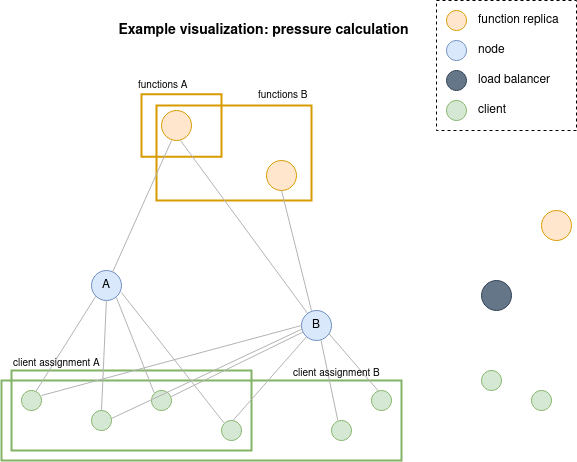
\includegraphics[width=12cm]{graphics/diagrams/client_lb_assignment.png}
    \caption{Assignment of clients and function replicas to potential load balancer nodes during pressure calculation}
    \label{fig:cl_lb_assignment}
\end{figure}
The request share is one of the central metrics we use to determine a node's pressure. In principle it shows which portion of the system's total incoming requests would be routed over that node, if it had a load balancer.
To calculate this value we need to first look at client assignment, meaning the process by which it is determined which client will send requests to which load balancer.

As we already outlined previously, one of our core assumptions is that clients will send their requests to whichever load balancer is closest from a network perspective, which is the load balancer with the shortest \gls{rtt}.
In keeping with our hypothetical scenario of "what if there was a load balancer on this node", clients will send their requests to this potential new load balancer if that node is closer to the clients than whichever load balancer instance is currently closest.
An example visualization of this client assignment for calculating request share can be seen in Figure \ref{fig:cl_lb_assignment}.
The specific number of clients our potential load balancer would service is, however, only of secondary importance. The more important and precise metric is the number of requests it will service.
We do not really care about whether there are a lot of clients sending few requests, or a low number of clients sending a large amount. What is important is only the number of requests going to the potential load balancer relative to the total amount sent.
Generally the data for this calculation is readily available, and can easily be gathered for example via existing load balancers reporting on the requests they receive.

A point to note here is that we only consider the requests sent within a certain time frame for this calculations, as they should be recent enough to be relevant for current scaling and scheduling decisions.
In our case we chose this time frame to be the last 60 seconds, which is relatively short but works within the relatively dynamic and heterogeneous systems we consider.
For real deployments this value might have to be adapted based on how dynamically the request load changes, how many requests each client typically sends in a session, and what amount of load is generally typical of the system.
The important point to consider here is that the time frame needs to be long enough to give a reasonably accurate picture, while not being so long that the data is delivers is not reflecting the current state of the system anymore.

Lastly, since there are multiple functions in the system, which we generally consider to be of equal importance, we calculate the request share the potential load balancer would receive on a per-function basis.
Thus we define the \textit{request share} as the following:
\DIFdelbegin \[ \DIFdel{\text{Let }N\text{ be the set of nodes,} }\]%DIFAUXCMD
\[ \DIFdel{L\text{ the set of nodes with running load balancer instances,} }\]%DIFAUXCMD
\[ \DIFdel{F\text{ the set of serverless functions,} }\]%DIFAUXCMD
\[ \DIFdel{\text{and }C\text{ the set of clients.} }\]%DIFAUXCMD
\[ \DIFdel{\text{Further let } dist(n,c) \text{ be the distance between a node } n \in N \text{ and client }c \in C\text{,}}\]%DIFAUXCMD
\[ \DIFdel{\text{ and let }requests(c, f) \text{ be the number of requests from client }c \in C \text{ for function }f \in F}\]%DIFAUXCMD
\[ \DIFdel{\text{Then for each node }n \in N\text{ the assigned clients are defined as} }\]%DIFAUXCMD
\DIFdelend \DIFaddbegin 

\DIFadd{Let $\mathbf{N}$ be the set of all nodes, $\mathbf{L}$ the set of nodes with running load balancer instances, $\mathbf{F}$ the set of deployed serverless functions, and $\mathbf{C}$ the set of clients.}\\
\DIFadd{Further let $\mathbf{dist(n,c)}$ be the distance between a node $\mathbf{n \in N}$ and client $\mathbf{c \in C}$, and let $\mathbf{requests(c, f)}$ be the number of requests from client $\mathbf{c \in C}$ for function $\mathbf{f \in F}$.}\\
\DIFadd{Then for each node $\mathbf{n \in N}$ the assigned clients are defined as
}\DIFaddend \[ assignment(n) = \{c | c \in C \land dist(c,n) < min\{dist(l, c) | l \in L\}\}\]
\DIFdelbegin \[ \DIFdel{\text{Finally the request share for node } n \in N \text{ for function }f \in F \text{ is defined as } }\]%DIFAUXCMD
\DIFdelend \DIFaddbegin \DIFadd{Finally the request share for node $\mathbf{n \in N}$ for function $\mathbf{f \in F}$ is defined as
}\DIFaddend \[ rqshare(n,f) = \frac{\sum_{c \in assignment(n)}requests(c,f)}{\sum_{c \in C}requests(c,f)}\]
\DIFaddbegin 


\DIFaddend Thus we define the request share of a node for a given function, as the fraction of all requests for that function the node would receive if it had a load balancer instance running.
\subsubsection{Projected Performance}
The second major metric that determines the pressure of a given node is what we refer to as the \textit{projected performance}.
This metric is once again based on the hypothetical scenario of "what if there was a load balancer on the given node" and is supposed to estimate the level of network performance we could expect if a load balancer is actually placed there.
Conceptually our notion of performance is rather simple.
It is determined by how close the clients are that would be assigned to that node, and by how close the function replicas are.
We once again calculate this metric for each node, and on a per-function basis.
To calculate the \textit{client distance} we use the average distance of all assigned clients, weighted by their relative share of requests among the assigned clients for the given function.

The calculation of the \textit{function distance} is somewhat more intricate.
Using a flat average over all function replicas is not a particularly suitable metric, since this would also consider the distance of function replicas that are far away, meaning that we would include the distance to function replicas we don't want the requests being sent to in the first place.
To address this issue we only consider a subsection of function replicas to calculate the function distance.
Our approach to the function distance is based on the assumption that the function scaling component correctly scales the function as required, meaning that we assume that the total number of function replicas is sufficient to serve the given number of incoming requests.
The number of function replicas we consider for a node is based on that nodes request share. We take into account the fraction of closest function replicas equal to the request share of the node for which we want to calculate the function distance.
If a node, for example, has a request share of 0.5, meaning 50\%, then its function distance is the average distance of the 50\% closest function replicas.
An example of this can once again be seen in Figure \ref{fig:cl_lb_assignment}, where nodes A and B have a differently sized share of functions assigned to them for distance calculation based on their respective request share.
Since we assume that the function replica scale is sufficient to handle the systems requests, this should mean that, not accounting for heterogeneity in function replica performance, the replicas considered for the function closeness metric are sufficient the incoming requests of the load balancer.
The reason we are not considering heterogeneity in replica performance is that this factor is not known beforehand, and in addition hard to estimate.
Finally we add the function distance and client distance together and invert them, since our subsequent calculations require the projected performance metric to have high values indicating good performance, and low values indicating poor performance.
Making this explicit we arrive at the following formulation for our projected performance:
\DIFdelbegin \[\DIFdel{\text{Let } replicas(f) \text{ be the set of replicas of a function }f \in F}\]%DIFAUXCMD
\[\DIFdel{\text{Then the client distance for a function }f \in F \text{ and node }n \in N \text{ is}}\]%DIFAUXCMD
\DIFdelend \DIFaddbegin 

\DIFadd{Let $\mathbf{replicas(f)}$ be the set of replicas of a function $\mathbf{f \in F}$.
Then the client distance for a function $\mathbf{f \in F}$ and node $\mathbf{n \in N}$ is
}\DIFaddend \[cldist(n,f) = \frac{\sum_{c \in assignment(n)}dist(n,c) \cdot requests(c,f)}{\sum_{c \in assignment(n)}requests(c,f)} \]
\DIFdelbegin \[\DIFdel{\text{Let }repdist_{n,f} = \langle r_{0}, r_{1}, ... \rangle \text{ be the list of replicas for a function }f \in F \text{ ordered by} }\]%DIFAUXCMD
\[\DIFdel{\text{their distance to }n \in N \text{ in ascending order such that for each pair } }\]%DIFAUXCMD
\DIFdelend \DIFaddbegin \DIFadd{Further, let $\mathbf{repdist_{n,f} = \langle r_{0}, r_{1}, ... \rangle}$ be the list of replicas for a function $\mathbf{f \in F}$ ordered by their distance to $\mathbf{n \in N}$ in ascending order such that for each pair 
}\DIFaddend \[(r_{i},r_{j}) \in repdist_{n,f}^{2}: i < j \implies dist(n, r_{i}) \leq dist(n, r_{j})\]
\DIFdelbegin \[\DIFdel{\text{Then the set of replicas considered is } }\]%DIFAUXCMD
\DIFdelend \DIFaddbegin \DIFadd{Then the set of replicas considered is
}\DIFaddend \[replicas(n,f) = \{r_{i} | r_{i} \in repdist_{n,f} \land i < \lfloor rqshare(n,f) \cdot |repdist_{n,r}| \rfloor\}\]
\DIFaddbegin \DIFadd{Thus the function distance is
}\DIFaddend \[\DIFdelbegin \DIFdel{\text{Thus the function distance is }}\DIFdelend fndist(n,f) = \frac{\sum_{r \in replicas(n,f)}dist(n,f)}{|replicas(n,f)|} \]
\DIFaddbegin \DIFadd{and finally, the projected performance is
}\DIFaddend \[\DIFdelbegin \DIFdel{\text{Finally the projected performance is }}\DIFdelend perf(n,f) = \frac{1}{cldist(n,f) + fndist(n,f)} \]
\DIFaddbegin 

\DIFaddend Needless to say slight adaptations of these formulas are necessary for a practical implementation.
For our simulator based evaluation the formulas are used exactly as we present them here, with the exception that special values are used as placeholders for undefined values, particularly those that result from a division by 0.
If a node has a request share of 0 for example, the projected performance is simply set to 0.
Likewise if the request share is > 0, the function distance calculation will take into account at least one replica, even if based on these formulas none would qualify.


\subsubsection{Pressure}
Now that we defined request shares and the projected performance we can move on to the actual pressure calculation.
In our approach we calculate what we call \textit{relative pressure}.
This means that the pressure of a given node is always in relation to the current state of the system, and not in absolutes.
This is done to ensure that the pressure calculation is not dependent on a-priori knowledge of the system.
If, for example, pressure were directly related to the number of requests per second the user would have to define what number of requests is considered high or low manually beforehand, negating precisely the kinds of advantage serverless frameworks are supposed to afford: Alleviating developers from complex configuration.

Our proposed notion of pressure is focused on the changes adding a load balancer on the node in question would bring to the system.
We start out by making an estimation of the average performance and impact of a load balancer in the system.
This notion of performance is based on the already described projected performance, and the load balancers request share.
We cannot rely purely on the projected performance, as it is also tremendously important for how many requests this performance is provided.
If we, for example, have a situation where we need to decide between two nodes which could potentially host a load balancer, that have a very high projected performance, then we most likely improve overall system performance more by selecting the node with the higher request share, since the high expected performance will affect more requests.

We call our estimation of the current system performance the \textit{status quo performance}.
To calculate it we once again rely on the projected performance, and the request share of node, although since we are interested in the current state of the system we consider these metrics only for nodes which currently host a load balancer.
The calculation of these metrics is exactly the same as for nodes that do not have load balancer instances deployed on them.
A slight difference to note is that the partition of clients onto nodes with load balancers will be without overlap, meaning that if we sum up all the request shares of a function over all nodes with a load balancer, the result would be 1, i.e. 100\%.

For our pressure metric this status quo performance is calculated using a weighted quantile.
The projected performance of the load balancer nodes are the values over which the quantile is calculated, while their respective request share is the weight.
We use the 50\% weighted quantile, also referred to as the weighted median, as our status quo performance.
In our testing the weighted median provided a robust metric that behaved predictably and similarly over different network topologies and cluster sizes.
It is, however, conceivable that there are situations in which this quantile should be set higher or lower depending on how dynamic the system changes, and how heterogeneous its structure and network topology are.
We should also note that at this point all of these metrics are still calculated on a per-function basis.
The values for each function are only combined at the very end, weighted by how important the individual functions are.
In our case the importance of individual functions is determined by which proportion of total requests are directed to it.
This means that we effectively treat each request as equally important and thus a function which gets double the traffic of another, for example, would also be considered twice as important when the individual function based metrics are combined.

% todo this should probably we rewritten a bit to be less repetitive
With this metric we can now calculate our pressure metric. For a given node we do this by calculating its impact on the system compared to the status quo performance.
Assuming that the status quo performance represents the current system performance overall, we compare the status quo performance with the performance of the system with the node added.
Since, as described earlier, the current set of load balancers services all client requests, adding a new load balancer will remove some of the traffic from existing load balancers.
This amount is represented by the potential load balancer node's request share.
To then calculate the system performance with the potential load balancer added we replace a part the size of the node's request share with the nodes performance.
Lastly we compare by how much adding a load balancer on this node changes the overall system performance, by calculating their difference in percent.
This percentage difference is the pressure value we use to make scaling and scheduling decisions in our osmotic system.
A positive pressure indicates that adding would likely improve performance, while negative pressure indicates that it would likely deteriorate overall system performance.
Thus we formally define our pressure as follows:
\DIFdelbegin \[\DIFdel{\text{For each function }f \in F \text{ it's relative importance is }}\]%DIFAUXCMD
\DIFdelend \DIFaddbegin 

\DIFadd{For each function $\mathbf{f \in F}$ its relative importance is
}\DIFaddend \[importance(f) = \frac{\sum_{c \in C}requests(c,f)}{\sum_{f' \in F}\sum_{c \in C}requests(c,f')} \]
\DIFdelbegin \[\DIFdel{\text{Let the set of tuples of a load balancer node's performance and request} }\]%DIFAUXCMD
\[ \DIFdel{\text{share for a function }f \in F \text{ be} }\]%DIFAUXCMD
\[\DIFdel{lbperf_{f} = \{(perf(l,f), rqshare(l,f)) | l \in L\} }\]%DIFAUXCMD
\[\DIFdel{\text{Then for a function the weighted median performance is } statusquo(f) = weightedmedian(lbperf_{f})}\]%DIFAUXCMD
\[\DIFdel{\text{Based on this we can estimate the system performance when adding a load balancer on node }n \in N}\]%DIFAUXCMD
\DIFdelend \DIFaddbegin \DIFadd{Let the set of tuples of a load balancer node's performance and request share for a function $\mathbf{f \in F}$ be $\mathbf{lbperf_{f}} = \{(perf(l,f), rqshare(l,f)) | l \in L\}$}\\
\DIFadd{Then for a function the weighted median performance is $\mathbf{statusquo(f)} = weightedmedian(lbperf_{f})$}\\
\DIFadd{Based on this we can estimated the systems performance when adding a load balancer on node $\mathbf{n \in N}$ as
}\DIFaddend \[ addperf(n,f) = (rqshare(n,f) * perf(n,f)) + ((1 - rqshare(n,f)) * statusquo(f))\]
\DIFdelbegin \[\DIFdel{\text{which relative to the status quo performance gives us the pressure per function} }\]%DIFAUXCMD
\DIFdelend \DIFaddbegin \DIFadd{which relative to the status quo performance gives us the pressure per function
}\DIFaddend \[ fp(n, f) = \frac{addperf(n,f) - statusquo(f)}{statusquo(f)}\]
\DIFaddbegin \DIFadd{Combined, the final pressure of the node is then
}\DIFaddend \[\DIFdelbegin \DIFdel{\text{Then combined the final pressure of the node is } }\DIFdelend p(n) = \sum_{f \in F}fp(n,f) \cdot importance(f)\]

\subsubsection{Downscaling Pressure}
Just like we need pressure to determine where load balancers should be scheduled, we also need to decide on conditions which trigger an existing load balancer to be removed.
Without this mechanic the osmotic scaling and scheduling component would not be able to properly adapt to changing system conditions, since load balancers that aren't placed effectively anymore cannot be removed.
During development we learned that an important property of the osmotic scaling and scheduling system is that it is consistent.
For our purposes this means that it should find a stable configuration eventually that doesn't change anymore unless the surrounding system parameters change.
In our testing the use of the exact same metric for removing load balancers as for adding them led to oscillations in their scheduling, meaning that there were cases were a load balancer would be added only to be removed again immediately.

To address this we use a slightly different measure of pressure for removing load balancer replicas.
It is also based on a hypothetical scenario, though in this case we try to estimate the consequences removing a load balancer would have on the system performance.
Compared to the pressure when adding load balancer replicas, we use a somewhat more accurate measure than for the removal process, since the original and future state of the system are more well known, considering it relies on more tangible and less hypothetical data.
First, the status quo before removal is calculated.
This is a weighted average of the projected performance of all load balancers weighted by their request share.
For the system performance once the load balancer is removed, we calculate how the system structure would change if the load balancer is removed.
The primary change this entails is that the removed load balancers clients would then send their requests to the next closest load balancer instance.
For simplicity and calculation efficiency, we assume that the clients would be assigned to whichever load balancer is closest to the one potentially getting removed.
At this point we recalculate the projected performance and request share of the load balancer that takes over the clients.
Based on this we can then calculate the system performance with the load balancer removed by again using a weighted average over the projected load balancer performances weighted by their request share, with the difference being that the load balancer we potentially remove is no longer counted, and its clients are moved to the next closest load balancer.
We then have an estimation of system performance with and without the load balancer in question, and go on to calculate their percentage difference.
This percentage difference tells us by how much removing the load balancer would affect overall system performance in percent, and based on a user defined threshold the scaler then decides to remove or keep each individual load balancer instance.
\DIFdelbegin \[\DIFdel{\text{For a function }f \in F \text{ the pre-removal status quo system performance is }}\]%DIFAUXCMD
\DIFdelend \DIFaddbegin 


\DIFadd{For a function $\mathbf{f \in F}$ the pre-removal status quo system performance is
}\DIFaddend \[rmstatusquo(f) = \sum_{l \in L}perf(l,f) \cdot rqshare(l,f)\]
\DIFdelbegin \[\DIFdel{\text{If we then remove a load balancer }l \in L \text{ the clients are taken over by another load balancer} }\]%DIFAUXCMD
\DIFdelend \DIFaddbegin \DIFadd{If we then remove a load balancer $\mathbf{l \in L}$ the clients are taken over by another load balancer
}\DIFaddend \[l': dist(l,l') \leq min\{dist(l,l'') | l'' \in L \setminus \{l\}\} \implies assignment(l') = assignment(l') \cup assignment(l)\]
\DIFdelbegin \[\DIFdel{\text{Giving us the adapted set of load balancers }L' = L \setminus \{l\} }\]%DIFAUXCMD
\[\DIFdel{\text{Then the system performance without the load balancer for a function is} }\]%DIFAUXCMD
\DIFdelend \DIFaddbegin \DIFadd{Giving us the adapted set of load balancers $\mathbf{L'} = L \setminus \{l\}$. Then the system performance without the load balancer for a function is
}\DIFaddend \[rmperf(l,f) = \sum_{l' \in L'}perf(l',f) \cdot rqshare(l',f) \]
\DIFdelbegin \[\DIFdel{\text{Based on which we can calculate the removal pressure per function as}}\]%DIFAUXCMD
\DIFdelend \DIFaddbegin \DIFadd{Based on which we can calculate the removal pressure per function as
}\DIFaddend \[ rmfp(l,f) = \frac{rmperf(l,f) - rmstatusquo(f)}{rmstatusquo(f)}\]
\DIFaddbegin \DIFadd{and combine the two to the final removal pressure
}\DIFaddend \[\DIFdelbegin \DIFdel{\text{and then combine them to the final removal pressure } }\DIFdelend rmp(l) = \sum_{f \in F}rmfp(l,f) \cdot importance(f)\]


\subsubsection{Throttled Scaling}
In our approach the scaling and scheduling components calculates pressures for all nodes and load balancers, and then makes subsequent scaling decisions, at a fixed interval.
While in theory multiple nodes could have a pressure beyond the set threshold that warrants adding a load balancer in a single interval, in our approach we artificially throttle this amount.
In our implementation of the scaling and scheduling component only a single load balancer can be added or removed per iteration.
We compensate for this comparatively slow rate of change by running the scaling and scheduling calculations at relatively short intervals.
There are two major reasons for our choice to limit the rate of change in the system in this way.

\begin{enumerate}
    \item The pressure metrics and calculation are based on the addition or removal of a single instance
    \item Since request shares potentially overlap, scheduling multiple load balancers often leads to immediate removal during the next scaling and scheduling cycle
\end{enumerate}

During development we observed faster convergence to a stable configuration when only adding or removing a single load balancer at a time.
We also considered changing our pressure calculations to optimize for a faster rate of change, but decided against it because these calculation are much less intuitive, which is detrimental to the ease of parametrization of the system, and most importantly the computational effort rises sharply with the number of load balancer instances that are considered simultaneously.
While the single node calculations we use only require calculating a maximum of 250 scenarios for a system with 250 nodes, the equivalent calculations for two nodes being scheduled simultaneously would require calculating up to 31125 scenarios for an equally sized system.
While this does limit the potential rate of change, we believe that a rate of change of about 4 load balancers per minute, which could still be increased if necessary, should be enough to handle the requirements of even comparatively dynamic systems.




%DIF >  target: 8-10ish pages
\DIFaddbegin \chapter{\DIFadd{Methodology}}
\DIFadd{The goal of this chapter is to give an overview of the general evaluation setup and methodology behind our approach, as this ties together the relation between our approach and its evaluation.
The approach we present is the result of several iterations of design and experimentation, as one would expect in the field of distributed systems engineering.
}

\DIFadd{First, we give an introduction to FaaS-Sim, the serverless edge computing simulator we use and extend and the devices included in the simulation.}\\
\DIFadd{Next we dive into more detail about the simulation setup by describing the serverless functions deployed, along with their performance characteristics.
In this section we also describe how the network simulation part of the simulator is implemented and how the network topologies used in the evaluations are structured.}\\
\DIFadd{From there we describe how empirical measurements and experiments are integrated in FaaS-Sim to improve its representation of real serverless systems.}\\
\DIFadd{Lastly, we conclude this chapter by outlining the metrics and \mbox{%DIFAUXCMD
\glspl{kpi} }\hskip0pt%DIFAUXCMD
captured in our simulation experiments.
}

\section{\DIFadd{Simulating Serverless Edge Computing Systems}}
\DIFadd{We choose FaaS-Sim\mbox{%DIFAUXCMD
\cite{faas-sim-github} }\hskip0pt%DIFAUXCMD
as our simulation framework.
FaaS-Sim is is a state of the art serverless computing simulation built on SimPy, %DIF > todo cite simpy
a discrete even simulation tool.
From an architectural basis, FaaS-Sim is built to mimic a serverless framework similar to OpenFaaS.
FaaS-Sim is built on top of a simulated Kubernetes infrastructure, meaning that it too has the notion of containers, container images, resource requirements, scaling, and scheduling.
Because FaaS-Sim is built with evaluating serverless edge computing in mind, it also includes support for representing a wide array of node hardware with heterogeneous capabilities and performance.
}\begin{table}[]
\begin{tabular}{lcccc}
\hline
\textbf{\DIFaddFL{Bin}}        & \textbf{\DIFaddFL{LOW}}  & \textbf{\DIFaddFL{MED}} & \textbf{\DIFaddFL{HIGH}} & \textbf{\DIFaddFL{VERY HIGH}} \\ \hline
\DIFaddFL{CPU Cores (logical) }& \DIFaddFL{1 - 2         }& \DIFaddFL{4 - 8        }& \DIFaddFL{16 - 32       }& \DIFaddFL{\textgreater 32    }\\
\DIFaddFL{Memory              }& \DIFaddFL{1 to 2        }& \DIFaddFL{4 - 8        }& \DIFaddFL{9 - 32        }& \DIFaddFL{\textgreater 32    }\\
\DIFaddFL{CPU Frequency (GHz) }& \DIFaddFL{\textless 1.5 }& \DIFaddFL{1.6 - 2.2    }& \DIFaddFL{\textless 3.5 }& \DIFaddFL{\textgreater 3.5   }\\ \hline
\end{tabular}
\caption{\DIFaddFL{Resource binning used for performance categorization and prediction with Ether devices by Raith, Rausch and Dustdar\mbox{%DIFAUXCMD
\cite{philipp-da}}\hskip0pt%DIFAUXCMD
}}
\label{tab:ether_bins}
\end{table}

\begin{table}[]
\begin{tabular}{lrrrrr}
\hline
\textbf{\begin{tabular}[c]{@{}l@{}}\DIFaddFL{Device}\\ \DIFaddFL{Name}\end{tabular}} & \textbf{\begin{tabular}[c]{@{}r@{}}\DIFaddFL{CPU}\\ \DIFaddFL{Arch}\end{tabular}} & \textbf{\begin{tabular}[c]{@{}r@{}}\DIFaddFL{CPU}\\ \DIFaddFL{Cores}\end{tabular}} & \textbf{\begin{tabular}[c]{@{}r@{}}\DIFaddFL{CPU}\\ \DIFaddFL{Freq}\end{tabular}} & \textbf{\begin{tabular}[c]{@{}r@{}}\DIFaddFL{Memory}\\ \DIFaddFL{GiB}\end{tabular}} & \textbf{\DIFaddFL{GPU/AI Accel}}   \\ \hline
\DIFaddFL{RPi3                                                           }& \DIFaddFL{arm32v7                                                     }& \DIFaddFL{4                                                            }& \DIFaddFL{LOW                                                         }& \DIFaddFL{1                                                             }& \DIFaddFL{-                       }\\
\DIFaddFL{RPi4                                                           }& \DIFaddFL{arm32v7                                                     }& \DIFaddFL{4                                                            }& \DIFaddFL{MED                                                         }& \DIFaddFL{1                                                             }& \DIFaddFL{-                       }\\
\DIFaddFL{RockPi                                                         }& \DIFaddFL{aarch64                                                     }& \DIFaddFL{6                                                            }& \DIFaddFL{MED                                                         }& \DIFaddFL{4                                                             }& \DIFaddFL{-                       }\\
\DIFaddFL{Coral                                                          }& \DIFaddFL{aarch64                                                     }& \DIFaddFL{4                                                            }& \DIFaddFL{MED                                                         }& \DIFaddFL{1                                                             }& \DIFaddFL{Google TPU co-processor }\\
\DIFaddFL{Intel NUC                                                            }& \DIFaddFL{x86\_64                                                     }& \DIFaddFL{4                                                            }& \DIFaddFL{MED                                                         }& \DIFaddFL{16                                                            }& \DIFaddFL{-                       }\\
\DIFaddFL{Jetson Xavier NX                                                             }& \DIFaddFL{aarch64                                                     }& \DIFaddFL{6                                                            }& \DIFaddFL{LOW                                                         }& \DIFaddFL{8                                                             }& \DIFaddFL{384-core Volta          }\\
\DIFaddFL{Jetson Nano                                                           }& \DIFaddFL{aarch64                                                     }& \DIFaddFL{4                                                            }& \DIFaddFL{LOW                                                         }& \DIFaddFL{4                                                             }& \DIFaddFL{128-core Maxwell        }\\
\DIFaddFL{Jetson TX2                                                           }& \DIFaddFL{aarch64                                                     }& \DIFaddFL{4                                                            }& \DIFaddFL{LOW                                                         }& \DIFaddFL{8                                                             }& \DIFaddFL{256-core Pascal        }\\
\DIFaddFL{Intel Xeon                                                           }& \DIFaddFL{x86\_64                                                     }& \DIFaddFL{4                                                            }& \DIFaddFL{HIGH                                                        }& \DIFaddFL{8                                                             }& \DIFaddFL{-                       }\\
\DIFaddFL{Intel Xeon + GPU                                                      }& \DIFaddFL{x86\_64                                                     }& \DIFaddFL{4                                                            }& \DIFaddFL{HIGH                                                        }& \DIFaddFL{8                                                             }& \DIFaddFL{Nvidia Turing GPU       }\\ \hline
\end{tabular}
\caption{\DIFaddFL{Table showing the simulated devices available in FaaS-Sim/Ether. CPU frequency bin sizes are shown in Table \ref{tab:ether_bins}}}
\label{tab:ether_devices}
\end{table}



\DIFadd{Table \ref{tab:ether_devices} shows an overview of the hardware devices our simulated clusters are comprised of.
}

\DIFadd{Scheduling in FaaS-Sim is based on the work of Rausch et al.\mbox{%DIFAUXCMD
\cite{skippy}}\hskip0pt%DIFAUXCMD
, and uses an exact re-implementation of the Kubernetes scheduler, making it an exact representation of that component's behaviour in real-life.
Scaling works like it does in OpenFaaS, meaning that functions can be scaled either via \mbox{%DIFAUXCMD
\gls{hpa} }\hskip0pt%DIFAUXCMD
or via OpenFaaS' trace driven approach.
Of course, the system also allows for custom and experimental scaling mechanisms to be integrated.
For some of our evaluations we do integrate such custom scaling behaviour, or more precisely the option to disable scaling at will, and to use a fixed replica counts instead, to remove this variability from certain evaluations if necessary.
}

\DIFadd{For the purposes of this work we extended FaaS-Sim to feature a second, parallel, and completely separate scaling and scheduling system.
As the placement of load balancers in serverless edge computing systems is one of the core aspects of this work, this second scaling and scheduling system is tasked only with determining the amount and location of load balancers.
All other parts of the serverless system are scaled and scheduled using the first system.
The two systems are entirely separate from each other, with the exception that they share the node resources containers are placed on.
}

\DIFadd{Being a serverless computing simulator, FaaS-Sim also includes the concept of functions.
Functions are, just like they are in OpenFaaS, an application running in a containerized fashion on the Kubernetes cluster, with a number of replicas determined by the scaler.
To simulate function invocations, particularly the \mbox{%DIFAUXCMD
\gls{fet} }\hskip0pt%DIFAUXCMD
component, FaaS-Sim relies on pre-defined statistical distributions to sample from.
For every request these distributions are sampled to determine the \mbox{%DIFAUXCMD
\gls{fet} }\hskip0pt%DIFAUXCMD
of the invocation.
FaaS-Sim supports the use of different distributions for each type of device present in the system, which allows FaaS-Sim to build on trace data from real-world deployments to make its own simulation more accurate.
For our evaluations, we build on the work done in this area by Raith, Rausch and Dustdar\mbox{%DIFAUXCMD
\cite{philipp-da}}\hskip0pt%DIFAUXCMD
.
FaaS-Sim also includes a model for performance degradation based on the computational capacity of the nodes, meaning that given a high enough request load single nodes become unable to handle all of them in reasonable time.
To provide some variability, we simulate a cluster that has three serverless functions deployed: }\textit{\DIFadd{Resnet50-Inference}}\DIFadd{, }\textit{\DIFadd{Mobilenet-Inference}}\DIFadd{, and }\textit{\DIFadd{Speech-Inference}}


\DIFadd{These functions all represent \mbox{%DIFAUXCMD
\gls{ai} }\hskip0pt%DIFAUXCMD
inference workloads as these the cornerstone to enabling edge intelligence\mbox{%DIFAUXCMD
\cite{rauschEdgeIntelligenceConvergence2019} }\hskip0pt%DIFAUXCMD
through serverless edge computing.
They are also an example of network bound workloads, usually featuring fast request processing, and are impacted significantly potential network congestion or long latencies.
}\begin{figure}
    \centering
    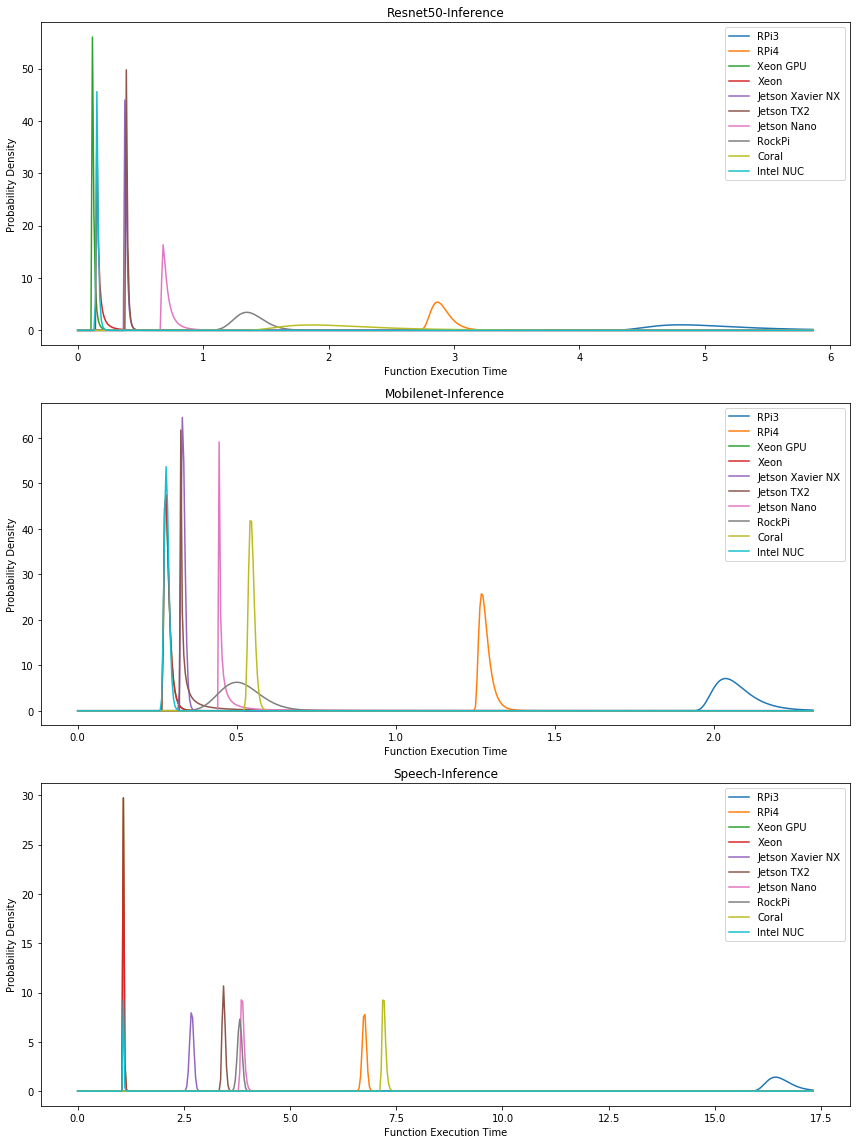
\includegraphics[width=\linewidth]{graphics/graphs/devices_fets.png}
    \caption{\DIFaddFL{Probability density functions of the \mbox{%DIFAUXCMD
\glspl{fet} }\hskip0pt%DIFAUXCMD
of the different devices we simulate}}
    \label{fig:devices_fets}
\end{figure}

\DIFadd{Figure \ref{fig:devices_fets}
shows the \mbox{%DIFAUXCMD
\gls{fet} }\hskip0pt%DIFAUXCMD
distributions for these functions on the hardware outlined in Table \ref{tab:ether_devices}.
}

\DIFadd{Because FaaS-Sim originally only supported response time evaluations due to \mbox{%DIFAUXCMD
\gls{fet}}\hskip0pt%DIFAUXCMD
, we extend it to also include the network time incurred from request transfers.
To enable this functionality, we introduce the notion of clients explicitly.
They are represented via nodes in the underlying network topology, just like the serverless cluster's nodes are.
Each request is dispatched from a client, sent to the nearest running load balancer instance, on to the function instance the load balancer selects, and back the same way.
}

\DIFadd{The load pattern clients exhibit in FaaS-Sim can be fully controlled.
Generally, clients follow a predefined request pattern, either individually or globally, but absolutely any pattern required can be implemented.
This allows the simulation of differently active clients, differently active regions, and request patterns that change depending on system parameters.
}

\DIFadd{To extract data for later analysis, FaaS-Sim features fine-grained and extensible trace-logging of all requests and system events.
}\section{\DIFadd{Network Simulation and Topologies}}
\DIFadd{Because this work places a particular emphasis on network optimization, the network simulation component of FaaS-Sim is of particular relevancy to us.
Under the hood, FaaS-Sim relies on Ether\mbox{%DIFAUXCMD
\cite{rausch-ether} }\hskip0pt%DIFAUXCMD
for its networking.
}

\DIFadd{Aside from vast option for customization, Ether supports a number of networking primitives that allow us to easily create a range of topologies.
In Ether's model, resources are usually, but not necessarily, grouped together in a cell.
The most important ones for our case are the }\textit{\DIFadd{LAN Cell}} \DIFadd{and the }\textit{\DIFadd{Shared Link Cell}}\DIFadd{.
The LAN Cell represents a set of compute nodes which are interconnected with each other in the way a LAN typically is, which means bandwidth is high, latency low, and variance small.}\\
\DIFadd{Contrary to that Shared Link Cells are more typical of what we might expect in an IoT scenario. 
It represents multiple nodes, which, as the name suggests, share a network connection between them.
This can, for example, be used to represent a number of edge devices which are grouped together into a small compute box and share a mobile internet connection for wider connectivity.
}

\DIFadd{The networking simulation in Ether is based around the }\textit{\DIFadd{Link}} \DIFadd{object\mbox{%DIFAUXCMD
\cite{rausch-ether}}\hskip0pt%DIFAUXCMD
, which represents a connection between nodes.
A mobile network connection, for example, would be considered a Link.
As Links represent connections, they also have a set bandwidth and latency.
To more accurately simulate how networks behave in real life, the latency of a link is not defined as a fixed number, but as a random distribution which gets sampled during simulation.
}

%DIF >  decided to do a textual representation, as it was more useful
%DIF >  this is just a placeholder in case I change my mind

\DIFadd{To simulate network transfers Ether uses a flow-based simulation.
The transfer of a request from one node to another is considered a flow.
For each flow two steps are simulated: TCP connection establishment, and data transfer.
TCP connection establishment is assumed to be equal to $ 3 \times \text{latency}$ of the route the flow takes, based on the three-way SYN, SYN-ACK, ACK handshake of the TCP protocol.}\\
\DIFadd{The data transfer is where the flow simulation component is used.
Each flow consists of a number of hops, connected by links.
Each of these links has a set latency, bandwidth, and potentially a number of other flows currently being transferred.
To calculate how long data transfer takes, we first determine the bandwidth.
The bandwidth is determined by the minimum bandwidth available from any of the flow's links.
What exactly this is depends on the general bandwidth of the link in question, and by how many flows have to share this available bandwidth.
Once the bandwidth of the flow is determined we can simply calculate how long data transfer will take, given a request of known size.
To preserve the impact different flows have on each other, once a flow is added to the system, or once a flow is completed and thus removed, every link of the flow is updated and potentially recalculates the bandwidth of other running flows.
Other flows might be unaffected, but may also see and increase or decrease in available bandwidth depending on whether there are now more or fewer flows competing.
If flows are competing for bandwidth, they are all treated with equal priority, and share equally in the available bandwidth.
}


\DIFadd{The topologies we use for our evaluations are based on the concept of smart cities\mbox{%DIFAUXCMD
\cite{suSmartCityApplications2011}}\hskip0pt%DIFAUXCMD
.
In this context we assume there may or may not be a central point in the city which provides a high amount of computational capability, i.e. a data center, and that the majority of computational capability will be interspersed throughout the city alongside with the clients.
}

\DIFadd{For these edge-located resources we assume that two major types exist: }\textit{\DIFadd{Smart Poles}} \DIFadd{and }\textit{\DIFadd{\mbox{%DIFAUXCMD
\gls{ran} }\hskip0pt%DIFAUXCMD
Towers}}\DIFadd{.
We consider \mbox{%DIFAUXCMD
\gls{ran} }\hskip0pt%DIFAUXCMD
Towers to be any type of LTE or 5G mobile base station, which in our smart city scenario would additionally be equipped with edge computing capability.
The Smart Poles we consider to be a functionally similar, though comparatively smaller device, much like the Huawei PoleStar\mbox{%DIFAUXCMD
\cite{huaweiPolestar}}\hskip0pt%DIFAUXCMD
, which is also equipped with computational capability, albeit less of it, and providing a connection to the wider network.
We assume that these Smart Poles would be spread out throughout the city like sensor nodes in the Array of Things\mbox{%DIFAUXCMD
\cite{catlettArrayThingsScientific2017a}}\hskip0pt%DIFAUXCMD
, a real world edge computing and smart city sensing deployment.
In terms of latency and bandwidth we assume latency to Smart Pole devices to be in the same ballpark as WiFi connections, while \mbox{%DIFAUXCMD
\gls{ran} }\hskip0pt%DIFAUXCMD
Tower connections are in line with what one would typically expect of LTE or 5G connections respectively.
In keeping with our methodology of informing simulation values with real world measurements where possible, we used the research conducted by Braud et al.\mbox{%DIFAUXCMD
\cite{braudMulticarrierMeasurementStudy2019} }\hskip0pt%DIFAUXCMD
and Nikravesh et al.\mbox{%DIFAUXCMD
\cite{nikraveshMobileNetworkPerformance2014a} }\hskip0pt%DIFAUXCMD
on real world LTE network characteristics to inform our parametrization of these connections.
We also assume that truly low latency connections for client devices are only provided by physically near access points such as the aforementioned Smart Pole devices, as research on wireless network technology indicates that there is a fundamental tradeoff between bandwidth, latency, and reliability\mbox{%DIFAUXCMD
\cite{soretFundamentalTradeoffsReliability2014}}\hskip0pt%DIFAUXCMD
.
}

\begin{figure}
    \centering
    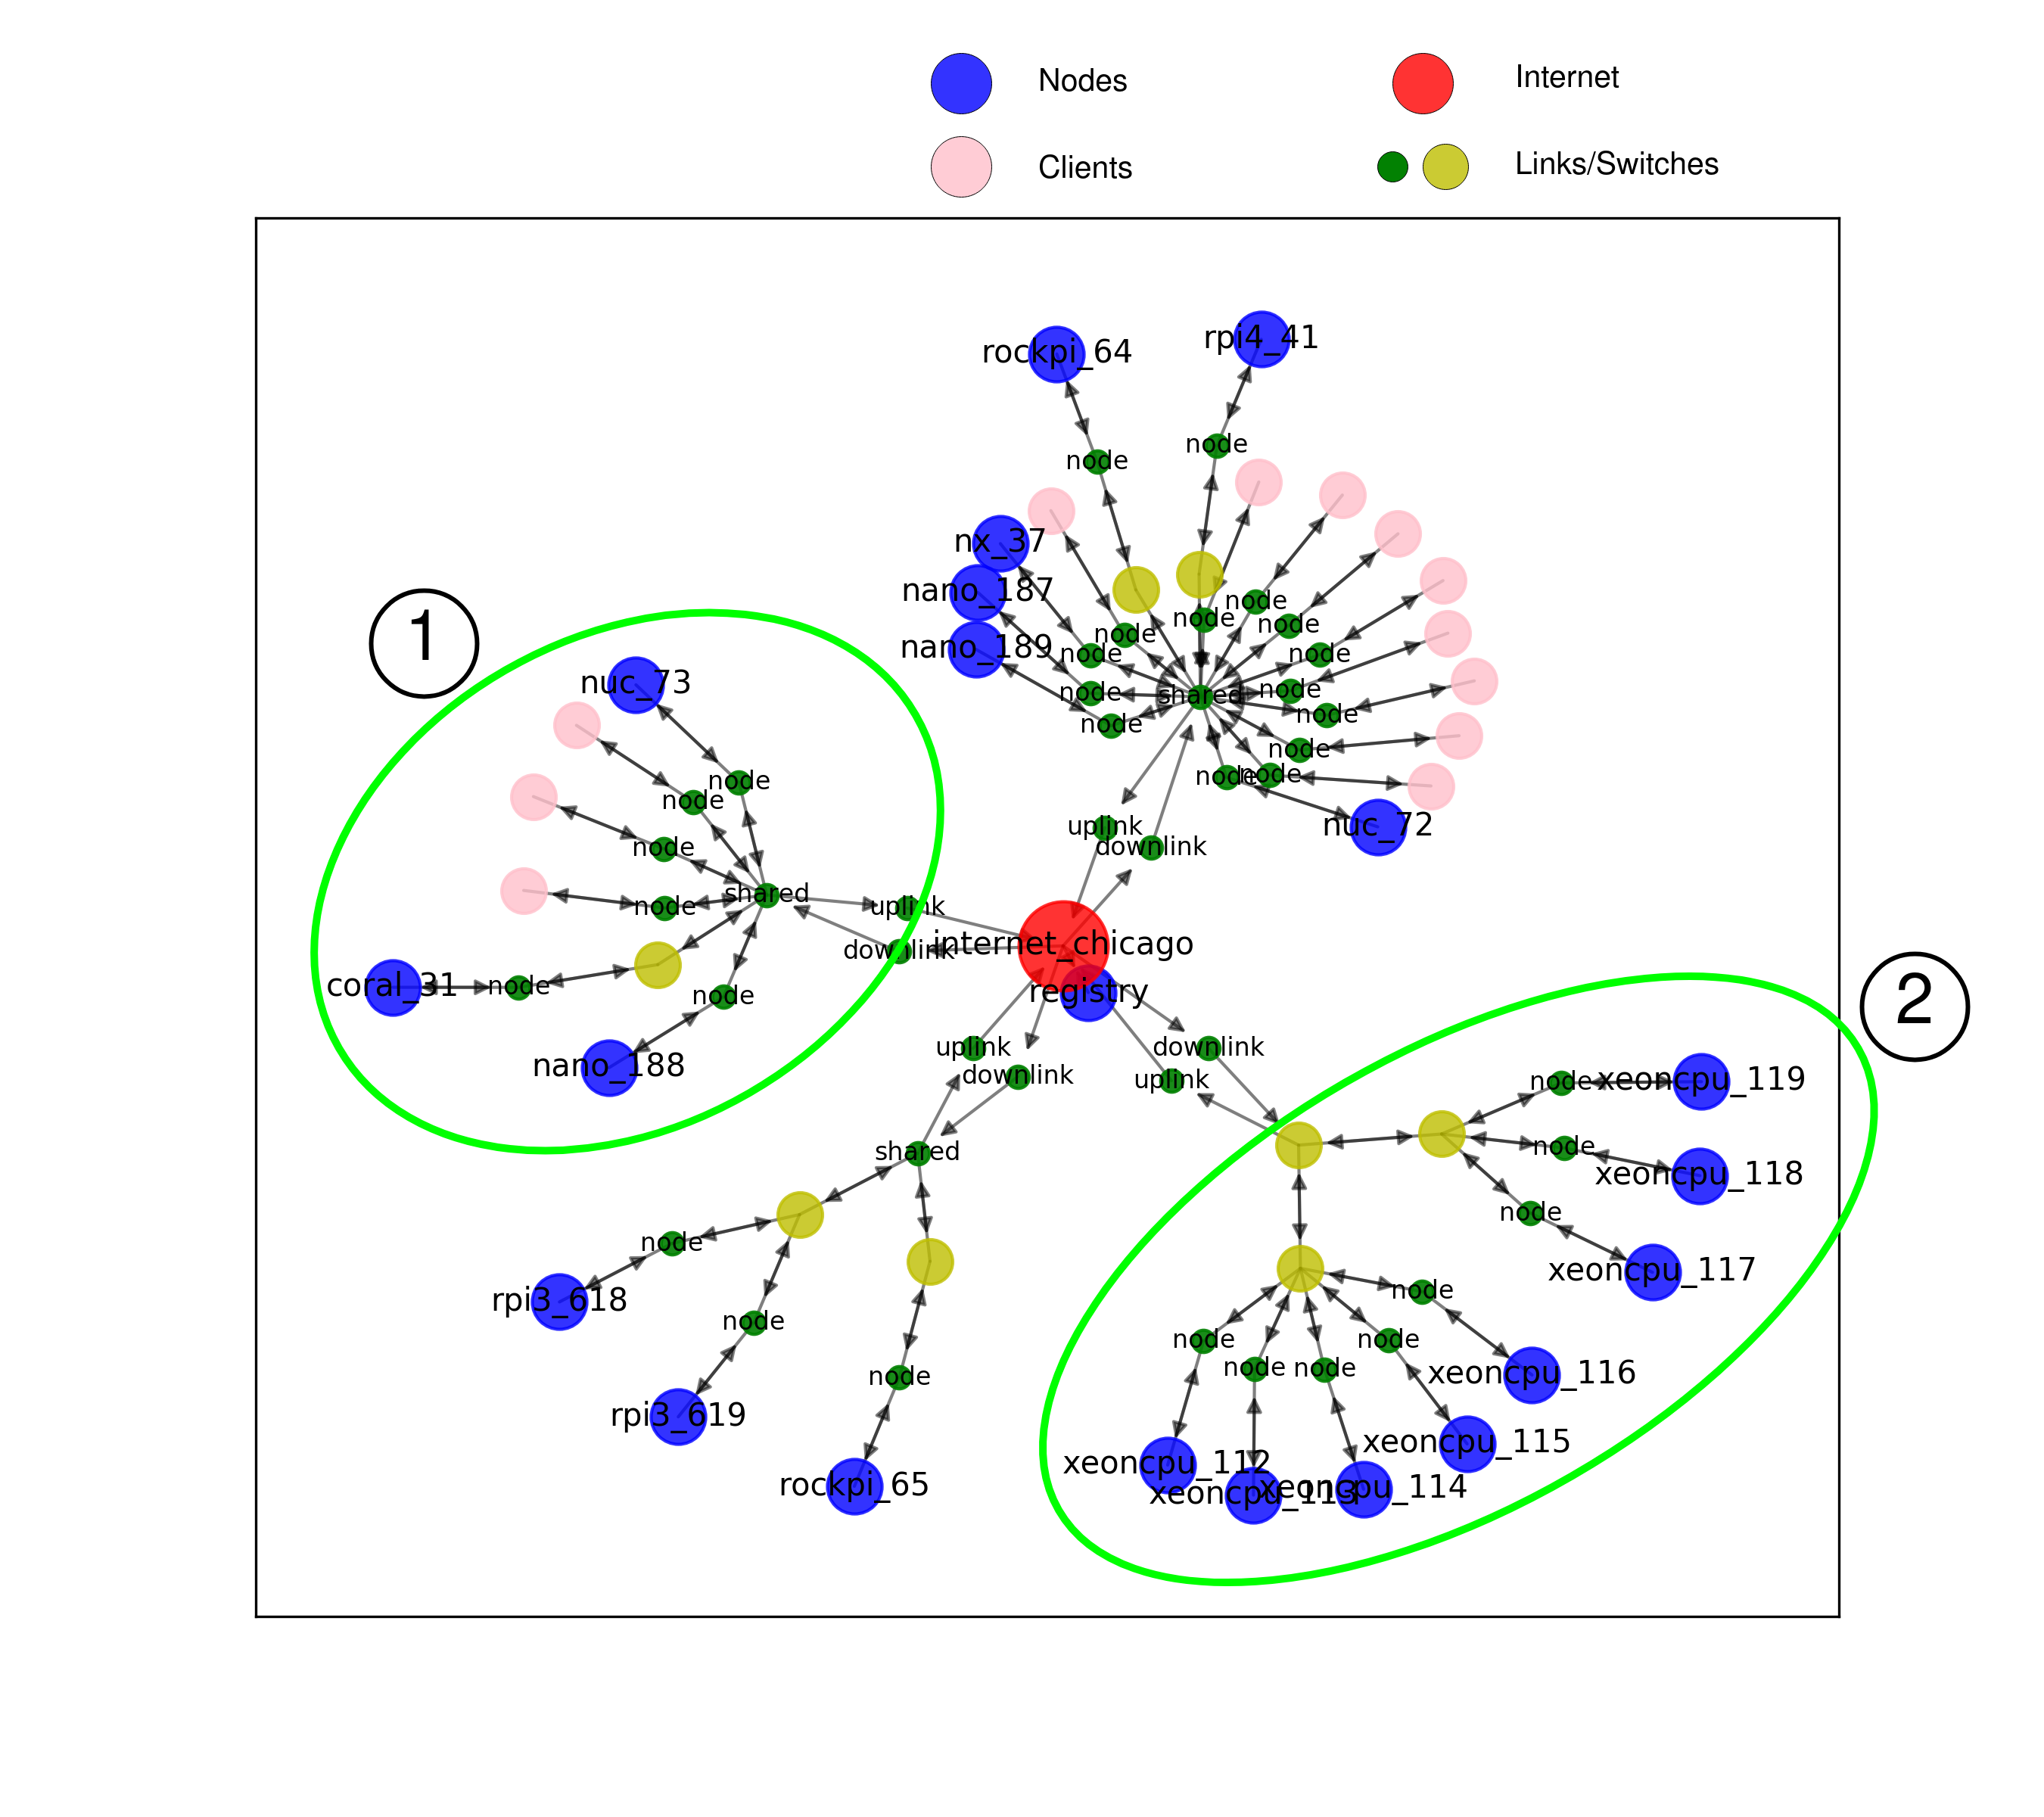
\includegraphics[width=\linewidth]{graphics/diagrams/tiny_topo.png}
    \caption{\DIFaddFL{Simplified network topology of a single smart city. Centered around the internet backbone uplink (red), 1) shows edge devices co-located with client devices. 2) shows a small cloud data center or cloudlet. Note the lack of clients directly connected to the cloudlet.}}
    \label{fig:tiny_topo}
\end{figure}

\DIFadd{Finally, Figure \ref{fig:tiny_topo} shows a simplified visualization of how one of our smart city topologies is structured.
Note that latency cannot be read from this visualization and that distances between nodes on the visualization do not correspond to network distances whatsoever.
The wider internet, presented as a red circle, is how communication to areas not deemed within the city, or general web-services such as container registries would be routed.
Also note that we only represent logical network links and connections in our topologies, which means that while in truth there might be tens of network hops between an edge node and the wider internet (e.g. through the nearest backbone uplink), for simulation performance reasons we do not include these in our model.
%DIF >  1 page
}\section{\DIFadd{Using Empirical Data in Simulations}}
\DIFadd{As already described FaaS-Sim\mbox{%DIFAUXCMD
\cite{faas-sim-github}}\hskip0pt%DIFAUXCMD
, the serverless simulator we use, is a trace-driven simulator\mbox{%DIFAUXCMD
\cite{thomas-thesis}}\hskip0pt%DIFAUXCMD
, meaning that it relies on measurements of real world data to make its results more representative.
The types of empirical data that can be used to improve simulation accuracy are very broad, but are typically limited to those that actually affect the metrics one is interested in measuring.
Usually this includes the memory consumption, CPU utilization, network utilization and storage size of different software components present in the system.
It can, however, also include more specific metrics such as deployment, staring, stopping and teardown times of container in a Kubernetes cluster\mbox{%DIFAUXCMD
\cite{skippy}}\hskip0pt%DIFAUXCMD
.
}

\DIFadd{Similar to how Raith et al. extended FaaS-Sim to include traces of real function executions to better represent \mbox{%DIFAUXCMD
\glspl{fet} }\hskip0pt%DIFAUXCMD
\mbox{%DIFAUXCMD
\cite{philipp-da}}\hskip0pt%DIFAUXCMD
, we perform experiments to inform how load balancers are modelled within the system.
Since in current serverless frameworks ingress-points, which is equivalent to a load balancer in our case, are considered as just another service, they compete with function replicas for resources.
As a result the resource usage of typical application level load balancers is an important metric for us to capture and integrate into the serverless simulator.
}

\DIFadd{For our empirical evaluations we use a real Kubernetes cluster that features a variety of heterogeneous nodes.
Since we deal with edge computing applications, and resource heterogeneity is a core challenge of edge computing\mbox{%DIFAUXCMD
\cite{shiEdgeComputingVisionChallenges2016}}\hskip0pt%DIFAUXCMD
, having a range of different nodes to evaluate performance on is critical to account for variance incurred by the use of different types of devices.
We also make use of and extend galileo\mbox{%DIFAUXCMD
\cite{galileo-github}}\hskip0pt%DIFAUXCMD
\mbox{%DIFAUXCMD
\cite{operating-energy-aware-galileo}}\hskip0pt%DIFAUXCMD
, a framework built for distributed load testing, as it allows us to easily define request patterns and loads that then get executed.
By using this we can go beyond measurements of baseline resource consumption and examine the relationship between the request load of a service and its performance and resource consumption profile.
To gather performance data of individual containers in a Kubernetes cluster, galileo relies on and integrates with telemd\mbox{%DIFAUXCMD
\cite{telemd-github}}\hskip0pt%DIFAUXCMD
.
Telemd is a daemon application that can gather a number of system metrics at specified intervals, including CPU utilization, memory consumption, disk I/O, and network transfers.
}


%DIF >  what do I actually want to say?
%DIF >  empirical experiments important to inform real world data
%DIF >  need to be aligned with the hardware simulated e.g. arm devices, x86, etc. etc.
%DIF >  this needs to be measured somehow -> galileo
%DIF > 
%DIF > 
%DIF >  1-2 pages
\section{\DIFadd{Captured Metrics}}
\DIFadd{There is a significant number of metrics that could be captured using such a simulation. With FaaS-Sim we capture traces of the requests being sent, and major system events.
The major system events are the addition or removal of deployments, as well as all scaling and scheduling decisions with respect to functions and load balancers.
For requests our traces provide the following information: \mbox{%DIFAUXCMD
\gls{trt}}\hskip0pt%DIFAUXCMD
, \mbox{%DIFAUXCMD
\gls{fet}}\hskip0pt%DIFAUXCMD
, waiting time, request client, load balancer instance, function instance, and the network times between client, load balancer and function instance.
The waiting time refers to the elapsed between a request having been received by a function instance, and the request being processed.
Waiting times occur if a node receives requests faster than it can process them.
In terms of resource usage, the resources reserved by the simulated Kubernetes pods, which correspond to the requirements defined in Kubernetes deployment manifests, are also recorded.
Note that this does not necessarily correspond to actual resource usage.
Because these reserved resource metrics are used for Kubernetes' scheduling decisions, we believe they are still worth being captured.
}

\DIFadd{In keeping with the set of potential metrics outlined by Aslanpour, Gill and Toosi\mbox{%DIFAUXCMD
\cite{aslanpourPerformanceEvaluationMetrics2020a}}\hskip0pt%DIFAUXCMD
, we pay particular attention to response times, potential \mbox{%DIFAUXCMD
\gls{sla} }\hskip0pt%DIFAUXCMD
levels and oscillation mitigation.
We also introduce more qualitative metrics, related to our particular evaluation scenario, such as the share of requests being routed outside of the city or network region they originate in.
}\DIFaddend % 10ish pages, about 8 in text, about 2 in figures
% Results had 18 pages, 50/50 ish split
% probably some 20ish pages here
\chapter{Evaluation}

% Stuff that goes here:
% Faas-sim: what is it, how does it work, what are its models, how does it deal with containers/kubernetes/openfaas/etc. What is simulated, what isn't? How are network flows simulated?
% Request pattern stuff.
% what types devices are there
% what functions are there, how do they perform on each device?
% image sizes, pulls, request payload sizes, all that stuff
% topologies: What are there and how are they built? real measurements from papers, etc. etc.
% -> city level, both old and modern, visualizations, etc.

% practical: how did we eval traefik
% real cluster, galileo (briefly), what devices are there? Auto-responder type app, payload size, response time, etc.

% Experiments:
% 1) Prelims
% 2) traefik resource eval
% 3) more realistic topo
% 4) load balancer count tests
% 5) LB hyperparameter tests
% 6) the osmotic stuffs?

\DIFdelbegin %DIFDELCMD < \newpage %%%
\DIFdelend \section{Initial Assessment}
% got 5,5-6 pages
This initial assessment is the first experiment we performed in the course of this work.
We performed it very early on to get an initial impression on whether our diagnosis of the problem, namely that load balancers are making ineffective decisions and are themselves located too far from clients, is accurate.
We also hoped to get a first impression of how large of a performance uplift might be achievable, and thus whether the performance improvement would justify the additional complexity our approach adds to the system.

The overarching question we want to answer with these experiments is whether more complex load balancing, such as least response time load balancing, and moving the load balancers closer to the clients leads to overall performance improvements.
We also want to understand what impact on performance we could expect from implementing only one of the two proposed improvements.

\DIFdelbegin \subsection{\DIFdel{Setup}}
%DIFAUXCMD
\addtocounter{subsection}{-1}%DIFAUXCMD
\DIFdelend \DIFaddbegin \subsubsection{\DIFadd{Setup}}
\DIFaddend To answer these questions we test four load balancer configurations in three different scenarios.
\DIFdelbegin \subsubsection{\DIFdel{Load Balancer Setup}}
%DIFAUXCMD
\addtocounter{subsubsection}{-1}%DIFAUXCMD
\DIFdelend \DIFaddbegin \paragraph{\DIFadd{Load Balancer Setup}}
\DIFaddend To assess the role of the load balancer implementation, we compare typical round robin load balancing, as it is found in current serverless frameworks such as OpenFaaS\cite{openfaas} and their underlying container orchestration service\cite{kubernetes}, and least response time load balancing to represent more sophisticated load balancing decisions.

Since this experiment is performed before the others we rely on an initial parametrization and implementation, which differs slightly from the one we ultimately propose.
The weight range is [1;10], with a scaling factor of 1, and a weight update interval of 15 seconds.
Furthermore we rely on a different implementation of weighted round robin\cite{wrr-kblinux}, which is functionally very similar but works through upstreams iteratively by their weight, instead of the more intermixed upstream selection we describe in our approach.
In this implementation, there is also a notion of current weights\cite{wrr-kblinux}, and they are reset every time the weights are updated.
\DIFdelbegin \subsubsection{\DIFdel{Load balancer scaling and placement}}
%DIFAUXCMD
\addtocounter{subsubsection}{-1}%DIFAUXCMD
\DIFdelend \DIFaddbegin \paragraph{\DIFadd{Load balancer scaling and placement}}
\DIFaddend For the load balancer location we evaluate the two most extreme scenarios: A single centralized load balancing instance which serves all client requests, and a maximally distributed scenario in which every single node in the system also hosts a load balancer instance.

This gives us four load balancer configurations:
\begin{itemize}
    \item Round Robin centralized
    \item Round Robin on all nodes
    \item Least Response Time centralized
    \item Least response time on all nodes
\end{itemize}

Each of these four configurations is evaluated in three different scenarios, which represent clusters of different size and network topology.
These topologies are oriented on a smart city/urban sensing type application.
\begin{itemize}
    \item City
    \item Nation
    \item Global
\end{itemize}
\DIFdelbegin \subsubsection{\DIFdel{City}}
%DIFAUXCMD
\addtocounter{subsubsection}{-1}%DIFAUXCMD
\DIFdelend \DIFaddbegin \paragraph{\DIFadd{City}}
\DIFaddend In this scenario the cluster is set to a size of 100 nodes, which are assumed to all be located in the same city, meaning network latencies between nodes are small.
The city features a data center which consists of about 50\% of the total node count, and features nodes with high compute capability, partially with GPU acceleration.
The rest of the nodes are assumed to be distributed across the city closer to clients, and consist to two thirds of medium performance nodes, and one third low performance nodes.
\DIFdelbegin \subsubsection{\DIFdel{Nation}}
%DIFAUXCMD
\addtocounter{subsubsection}{-1}%DIFAUXCMD
\DIFdelend \DIFaddbegin \paragraph{\DIFadd{Nation}}
\DIFaddend This scenario features a larger cluster that spans over three cities.
Each of those cities features the same relative node distribution as the previous scenario.
We chose the USA as our example, as using a small country such as Austria would not provide significant enough latency differences between cities.
Our scenario features the cities of Chicago with 100 nodes, Seattle with 100 nodes, and New York with 150 nodes.
While nodes within the same city feature extremely low network latency, nodes across two cities have more significant network distances between them.

 \begin{table}[]
\centering
\begin{tabular}{r|ccc}
\multicolumn{1}{c|}{} & \textbf{Chicago} & \textbf{New York} & \textbf{Seattle} \\ \hline
\textbf{Chicago}      & -                & 31ms              & 55ms             \\
\textbf{New York}     & 31ms             & -                 & 75ms             \\
\textbf{Seatte}       & 55ms             & 75ms              & -                \\ \hline
\end{tabular}
\caption{Network latencies between cities in the initial \textbf{nation} evaluation scenario. Latencies are taken from Wonder Network's global ping statistics\cite{wondernetworkGlobalPingStatistics}}
\label{tab:initial_nation_pings}
\end{table}

\begin{table}[]
\centering
\begin{tabular}{r|ccc}
\multicolumn{1}{c|}{} & \textbf{New York} & \textbf{London} & \textbf{Sydney} \\ \hline
\textbf{New York}     & -                 & 86ms            & 204ms           \\
\textbf{London}       & 86ms              & -               & 253ms           \\
\textbf{Sydney}       & 204ms             & 253ms           & -               \\ \hline
\end{tabular}

\caption{Network latencies between cities in the initial \textbf{global} evaluation scenario. Latencies are taken from Wonder Network's global ping statistics\cite{wondernetworkGlobalPingStatistics}}
\label{tab:initial_global_pings}
\end{table}   

The network latencies between the cities are taken from Wonder Network\cite{wondernetworkGlobalPingStatistics}, and can be seen in Table \ref{tab:initial_nation_pings}

\DIFdelbegin \subsubsection{\DIFdel{Global}}
%DIFAUXCMD
\addtocounter{subsubsection}{-1}%DIFAUXCMD
\DIFdelend \DIFaddbegin \paragraph{\DIFadd{Global}}
\DIFaddend The global scenario once again features three cities, but they are distributed not just within a single country, but across the globe.
The cities are New york with 100 nodes, London with 100 nodes, and Sydney with 150 nodes.
Network latencies can be seen in Table \ref{tab:initial_global_pings}.

\DIFdelbegin \subsubsection{\DIFdel{Clients}}
%DIFAUXCMD
\addtocounter{subsubsection}{-1}%DIFAUXCMD
\DIFdelend \DIFaddbegin \paragraph{\DIFadd{Clients}}
\DIFaddend Each scenarios features a client ratio of 0.6, meaning there are 60\% as many clients as there are compute nodes.
Clients are assumed to be on the edge of the network and thus closest to the medium and small sized compute nodes.

\DIFdelbegin \subsubsection{\DIFdel{Functions and request load}}
%DIFAUXCMD
\addtocounter{subsubsection}{-1}%DIFAUXCMD
\DIFdelend \DIFaddbegin \paragraph{\DIFadd{Functions and request load}}
\DIFaddend We used our basic three function deployments for these experiments.
To isolate the system behaviour on the effect of load balancer implementation, scale and placement we disabled the normal function scaling behaviour.
Instead the system immediately sets a fixed scale for each function such that for each node in the entire cluster a function replica is started.
We consider the functions to be of equal importance, thus each function starts up $\frac{n}{3}$ replicas where $n$ is the total number of nodes.
Lastly all experiments simulate a timeframe of 1000 seconds, and feature a request load of 75\gls{rps}.

\DIFdelbegin \subsection{\DIFdel{Results}}
%DIFAUXCMD
\addtocounter{subsection}{-1}%DIFAUXCMD
\DIFdelend \DIFaddbegin \subsubsection{\DIFadd{Results}}
\DIFaddend 

\begin{table}[]
\begin{tabular}{lrrrr}
\hline
                                 & \multicolumn{4}{c}{mean}                                                                                                                              \\
\textbf{Load Balancer Type}      & \multicolumn{1}{r}{\textbf{TRT}} & \multicolumn{1}{r}{\textbf{FET}} & \multicolumn{1}{r}{\textbf{Net CL-LB}} & \multicolumn{1}{r}{\textbf{Net LB-FX}} \\ \hline
\multicolumn{5}{c}{City Scale Evaluation}                                                                                                                                                \\ \hline
Round Robin centralized          & 0.0\%                            & 0.0\%                            & 0.0\%                                  & 0.0\%                                  \\
Round Robin on all nodes         & 13.3\%                           & 0.0\%                            & 35.4\%                                 & 30.3\%                                 \\
Least Response Time centralized  & 32.7\%                           & 47.9\%                           & 15.8\%                                 & 24.6\%                                 \\
Least Response Time on all nodes & 81.3\%                           & 109.3\%                          & 51.6\%                                 & 61.9\%                                 \\ \hline
\multicolumn{5}{c}{Nation Scale Evaluation}                                                                                                                                              \\ \hline
Round Robin centralized          & 0.0\%                            & 0.0\%                            & 0.0\%                                  & 0.0\%                                  \\
Round Robin on all nodes         & 95.7\%                           & -0.4\%                           & 1028.2\%                               & 34.8\%                                 \\
Least Response Time centralized  & 18.1\%                           & 27.8\%                           & 3.0\%                                  & 34.7\%                                 \\
Least Response Time on all nodes & 312.0\%                          & 86.9\%                           & 1065.6\%                               & 257.5\%                                \\ \hline
\multicolumn{5}{c}{Global Scale Evaluation}                                                                                                                                              \\ \hline
Round Robin centralized          & 0.0\%                            & 0.0\%                            & 0.0\%                                  & 0.0\%                                  \\
Round Robin on all nodes         & 82.8\%                           & -0.7\%                           & 2910.6\%                               & -5.3\%                                 \\
Least Response Time centralized  & 21.0\%                           & 18.4\%                           & 0.0\%                                  & 60.8\%                                 \\
Least Response Time on all nodes & 606.9\%                          & 77.3\%                           & 2997.8\%                               & 428.2\%                                \\ \hline
\end{tabular}
\caption{Mean values of a single experimental run of the initial evaluation in different scenarios. Displayed values are in order: Total response time, function execution time, network time between client and load balancer, and network time between load balancer and function replica}
\label{tab:initial_eval_results_mean}
\end{table}

\begin{table}[]
\begin{tabular}{lrrrr}
\hline
                                 & \multicolumn{4}{c}{50th percentile (median)}                                                                                                          \\
\textbf{Load Balancer Type}      & \multicolumn{1}{r}{\textbf{TRT}} & \multicolumn{1}{r}{\textbf{FET}} & \multicolumn{1}{r}{\textbf{Net CL-LB}} & \multicolumn{1}{r}{\textbf{Net LB-FX}} \\ \hline
\multicolumn{5}{c}{City Scale Evaluation}                                                                                                                                                \\ \hline
Round Robin centralized          & 0.0\%                            & 0.0\%                            & 0.0\%                                  & 0.0\%                                  \\
Round Robin on all nodes         & 26.5\%                           & 0.0\%                            & 34.0\%                                 & 25.1\%                                 \\
Least Response Time centralized  & 34.8\%                           & 183.0\%                          & 5.0\%                                  & 13.5\%                                 \\
Least Response Time on all nodes & 93.3\%                           & 185.6\%                          & 37.0\%                                 & 37.7\%                                 \\ \hline
\multicolumn{5}{c}{Nation Scale Evaluation}                                                                                                                                              \\ \hline
Round Robin centralized          & 0.0\%                            & 0.0\%                            & 0.0\%                                  & 0.0\%                                  \\
Round Robin on all nodes         & 109.0\%                          & -7.9\%                           & 1674.1\%                               & 76.2\%                                 \\
Least Response Time centralized  & 23.5\%                           & 16.1\%                           & 4.3\%                                  & 118.2\%                                \\
Least Response Time on all nodes & 350.4\%                          & 22.9\%                           & 1674.1\%                               & 1316.4\%                               \\ \hline
\multicolumn{5}{c}{Global Scale Evaluation}                                                                                                                                              \\ \hline
Round Robin centralized          & 0.0\%                            & 0.0\%                            & 0.0\%                                  & 0.0\%                                  \\
Round Robin on all nodes         & 27.6\%                           & 0.0\%                            & 5338.8\%                               & 95.0\%                                 \\
Least Response Time centralized  & 9.8\%                            & 0.6\%                            & 0.0\%                                  & 1498.5\%                               \\
Least Response Time on all nodes & 1653.3\%                         & 25.9\%                           & 5338.8\%                               & 4541.5\%                               \\ \hline
\end{tabular}
\caption{50th percentile (i.e. median) values of a single experimental run of the initial evaluation in different scenarios. Displayed values are in order: Total response time, function execution time, network time between client and load balancer, and network time between load balancer and function replica}
\label{tab:initial_eval_results_q50}
\end{table}

\DIFdelbegin %DIFDELCMD < \begin{figure}
%DIFDELCMD <     \centering
%DIFDELCMD <     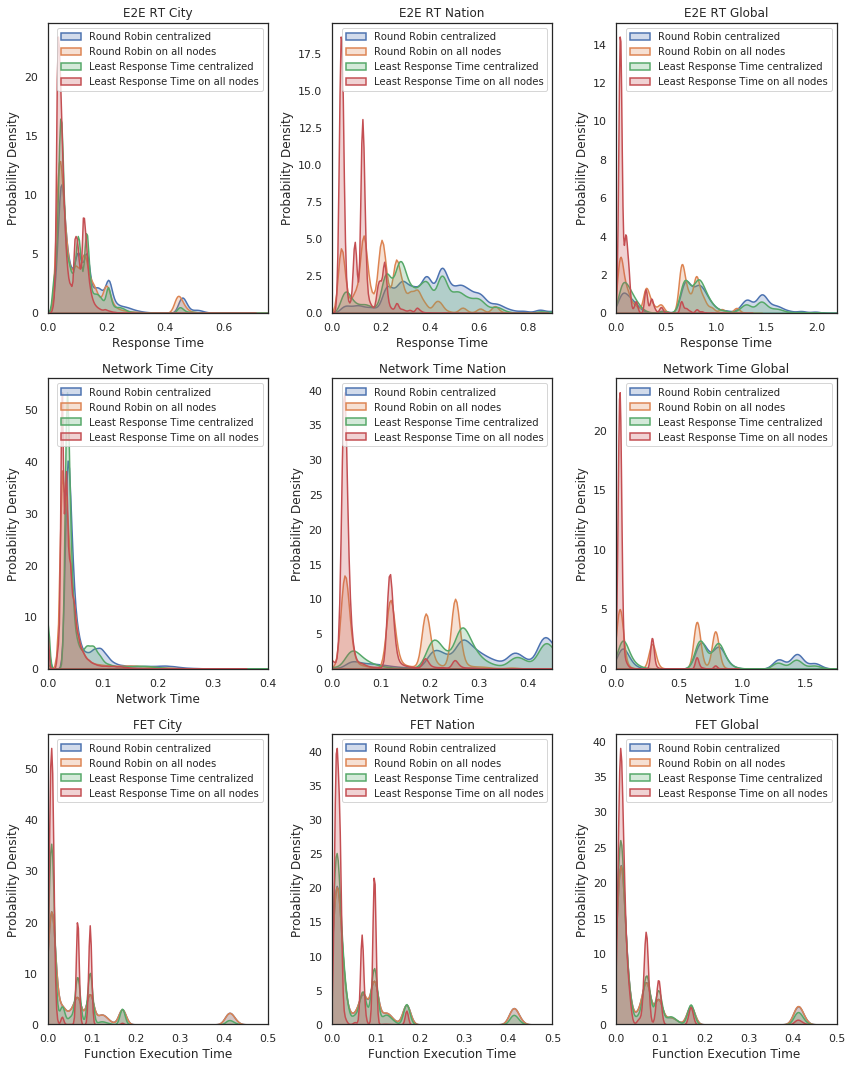
\includegraphics[width=\linewidth]{graphics/graphs/initial_eval_pdfs_3x3.png}
%DIFDELCMD <     %%%
%DIFDELCMD < \caption{%
{%DIFAUXCMD
\DIFdelFL{Kernel Density Estimate of a single experiment run. Shown data can be interpreted as probability density functions. Data is visualized for \mbox{%DIFAUXCMD
\gls{trt}}\hskip0pt%DIFAUXCMD
, \mbox{%DIFAUXCMD
\gls{fet} }\hskip0pt%DIFAUXCMD
and the time incurred through network transfers.}}
    %DIFAUXCMD
%DIFDELCMD < \label{fig:initial_eval_pdfs}
%DIFDELCMD < \end{figure}
%DIFDELCMD < 

%DIFDELCMD < %%%
\DIFdelend Since the experiments feature a significant degree of random sampling in their simulation, we ran each experiment 10 times.
The results presented here are those of a single experimental run, since no runs showed significantly different results.
Table \ref{tab:initial_eval_results_mean} shows the percentage improvement different load balancer types and scales give when compared to the default centralized round robin.
Here the mean values of the \gls{trt}, \gls{fet}, and network times between client and load balancer, and load balancer and function replica are shown.
Both a more sophisticated approach to load balancing and moving load balancer instances closer to the clients shows significant performance improvements, but across the board only the combination of these two improvements (i.e. least response time on all nodes) gives the most significant performance uplift.
We can also see that least response time load balancing not only improves network times between the load balancer and the function replica, but also decreases \DIFdelbegin \DIFdel{\ref{fet}}\DIFdelend \DIFaddbegin \DIFadd{\mbox{%DIFAUXCMD
\gls{fet}}\hskip0pt%DIFAUXCMD
}\DIFaddend .
In addition we observe that the performance improvement given through distributed least response time load balancing becomes larger in geographically more distributed scenarios.

Table \ref{tab:initial_eval_results_q50} shows the difference between the median of these metrics.
Here the performance uplift achieved by least response time load balancing on all nodes become even larger, up to a 16,5x improvement in \gls{trt} in the global scenario.

For even more detailed analyses figure \ref{fig:initial_eval_pdfs} shows the probability density function estimated of the same experimental run.
Note that \textit{E2E RT} in this figure means \gls{trt}.
Here the overall trend observed in the tables \ref{tab:initial_eval_results_mean} and \ref{tab:initial_eval_results_q50} carries through, showing that least response time on all nodes not only improves average performance, but pushes the whole distribution towards faster \gls{fet} and lower network times.
\DIFdelbegin %DIFDELCMD < \newpage 
%DIFDELCMD <  \newpage %%%
\DIFdelend \DIFaddbegin 

\DIFaddend \section{\DIFdelbegin \DIFdel{Least Response Time }\DIFdelend Load \DIFdelbegin \DIFdel{Balancing }\DIFdelend \DIFaddbegin \DIFadd{Balancer }\DIFaddend Implementation \DIFaddbegin \DIFadd{and Parametrization}\DIFaddend }
\DIFaddbegin \subsection{\DIFadd{Least Response Time Load Balancing Implementation}}
\DIFaddend % got 2,5 pages
With these experiments the goal is to better understand how the implementation details of the load balancing solution affect overall performance.
The previously performed initial evaluation revealed some potentially counter-intuitive behaviour, so to better inform our proposed implementation these experiments evaluate different implementation patterns.

An implementation of least response time load balancing is split in two parts: The gathering of response time data, and the conversion of that data into load balancing decisions.
As we discussed in our approach, we convert the response time data into weights, which are used as inputs to a weighted round robin load balancing implementation that ultimately makes load balancing decisions.
\DIFdelbegin \subsection{\DIFdel{Setup}}
%DIFAUXCMD
\addtocounter{subsection}{-1}%DIFAUXCMD
\DIFdelend \DIFaddbegin \subsubsection{\DIFadd{Setup}}
\DIFaddend With these experiments our focus lies on these implementations of weighted round robin.
In particular we evaluate four different implementations of weighted round robin:
\begin{itemize}
    \item \textbf{Random:} this implementation uses a simple weighted random distribution. It is used as a baseline to compare other implementations to
    \item \textbf{Classic:} this represents the implementation used in the initial evaluation experiment\cite{wrr-kblinux}. It is deterministic and works through upstreams starting with the ones with the highest weight.
    \item \textbf{Adapted Classic:} the same implementation as classic, but it does not reset its internal state when weights are updated. 
    \item \textbf{Smooth:} the implementation described in our approach and also used by nginx\cite{nginx-wrr}. It too is deterministic but alternates between upstreams with high and low weights in load balancing decisions.
\end{itemize}

We simulate a least response time load balancer with each of these implementations with 500 upstreams, which are simplified to sample response times from a lognormal distribution, over a timeframe of 500 seconds with a request rate of 5\gls{rps}.
Weights are updated every 15 seconds, except for the smooth weighted round robin implementation which is updated every second, since this is a core benefit afforded by the implementation we want to test explicitly.
The weight range for each implementation is [0;10] and response times get mapped linearly, i.e. using a scaling factor of 1.

\DIFdelbegin \subsection{\DIFdel{Results}}
%DIFAUXCMD
\addtocounter{subsection}{-1}%DIFAUXCMD
\DIFdelend \DIFaddbegin \subsubsection{\DIFadd{Results}}
\DIFaddend 

\begin{figure}
    \centering
    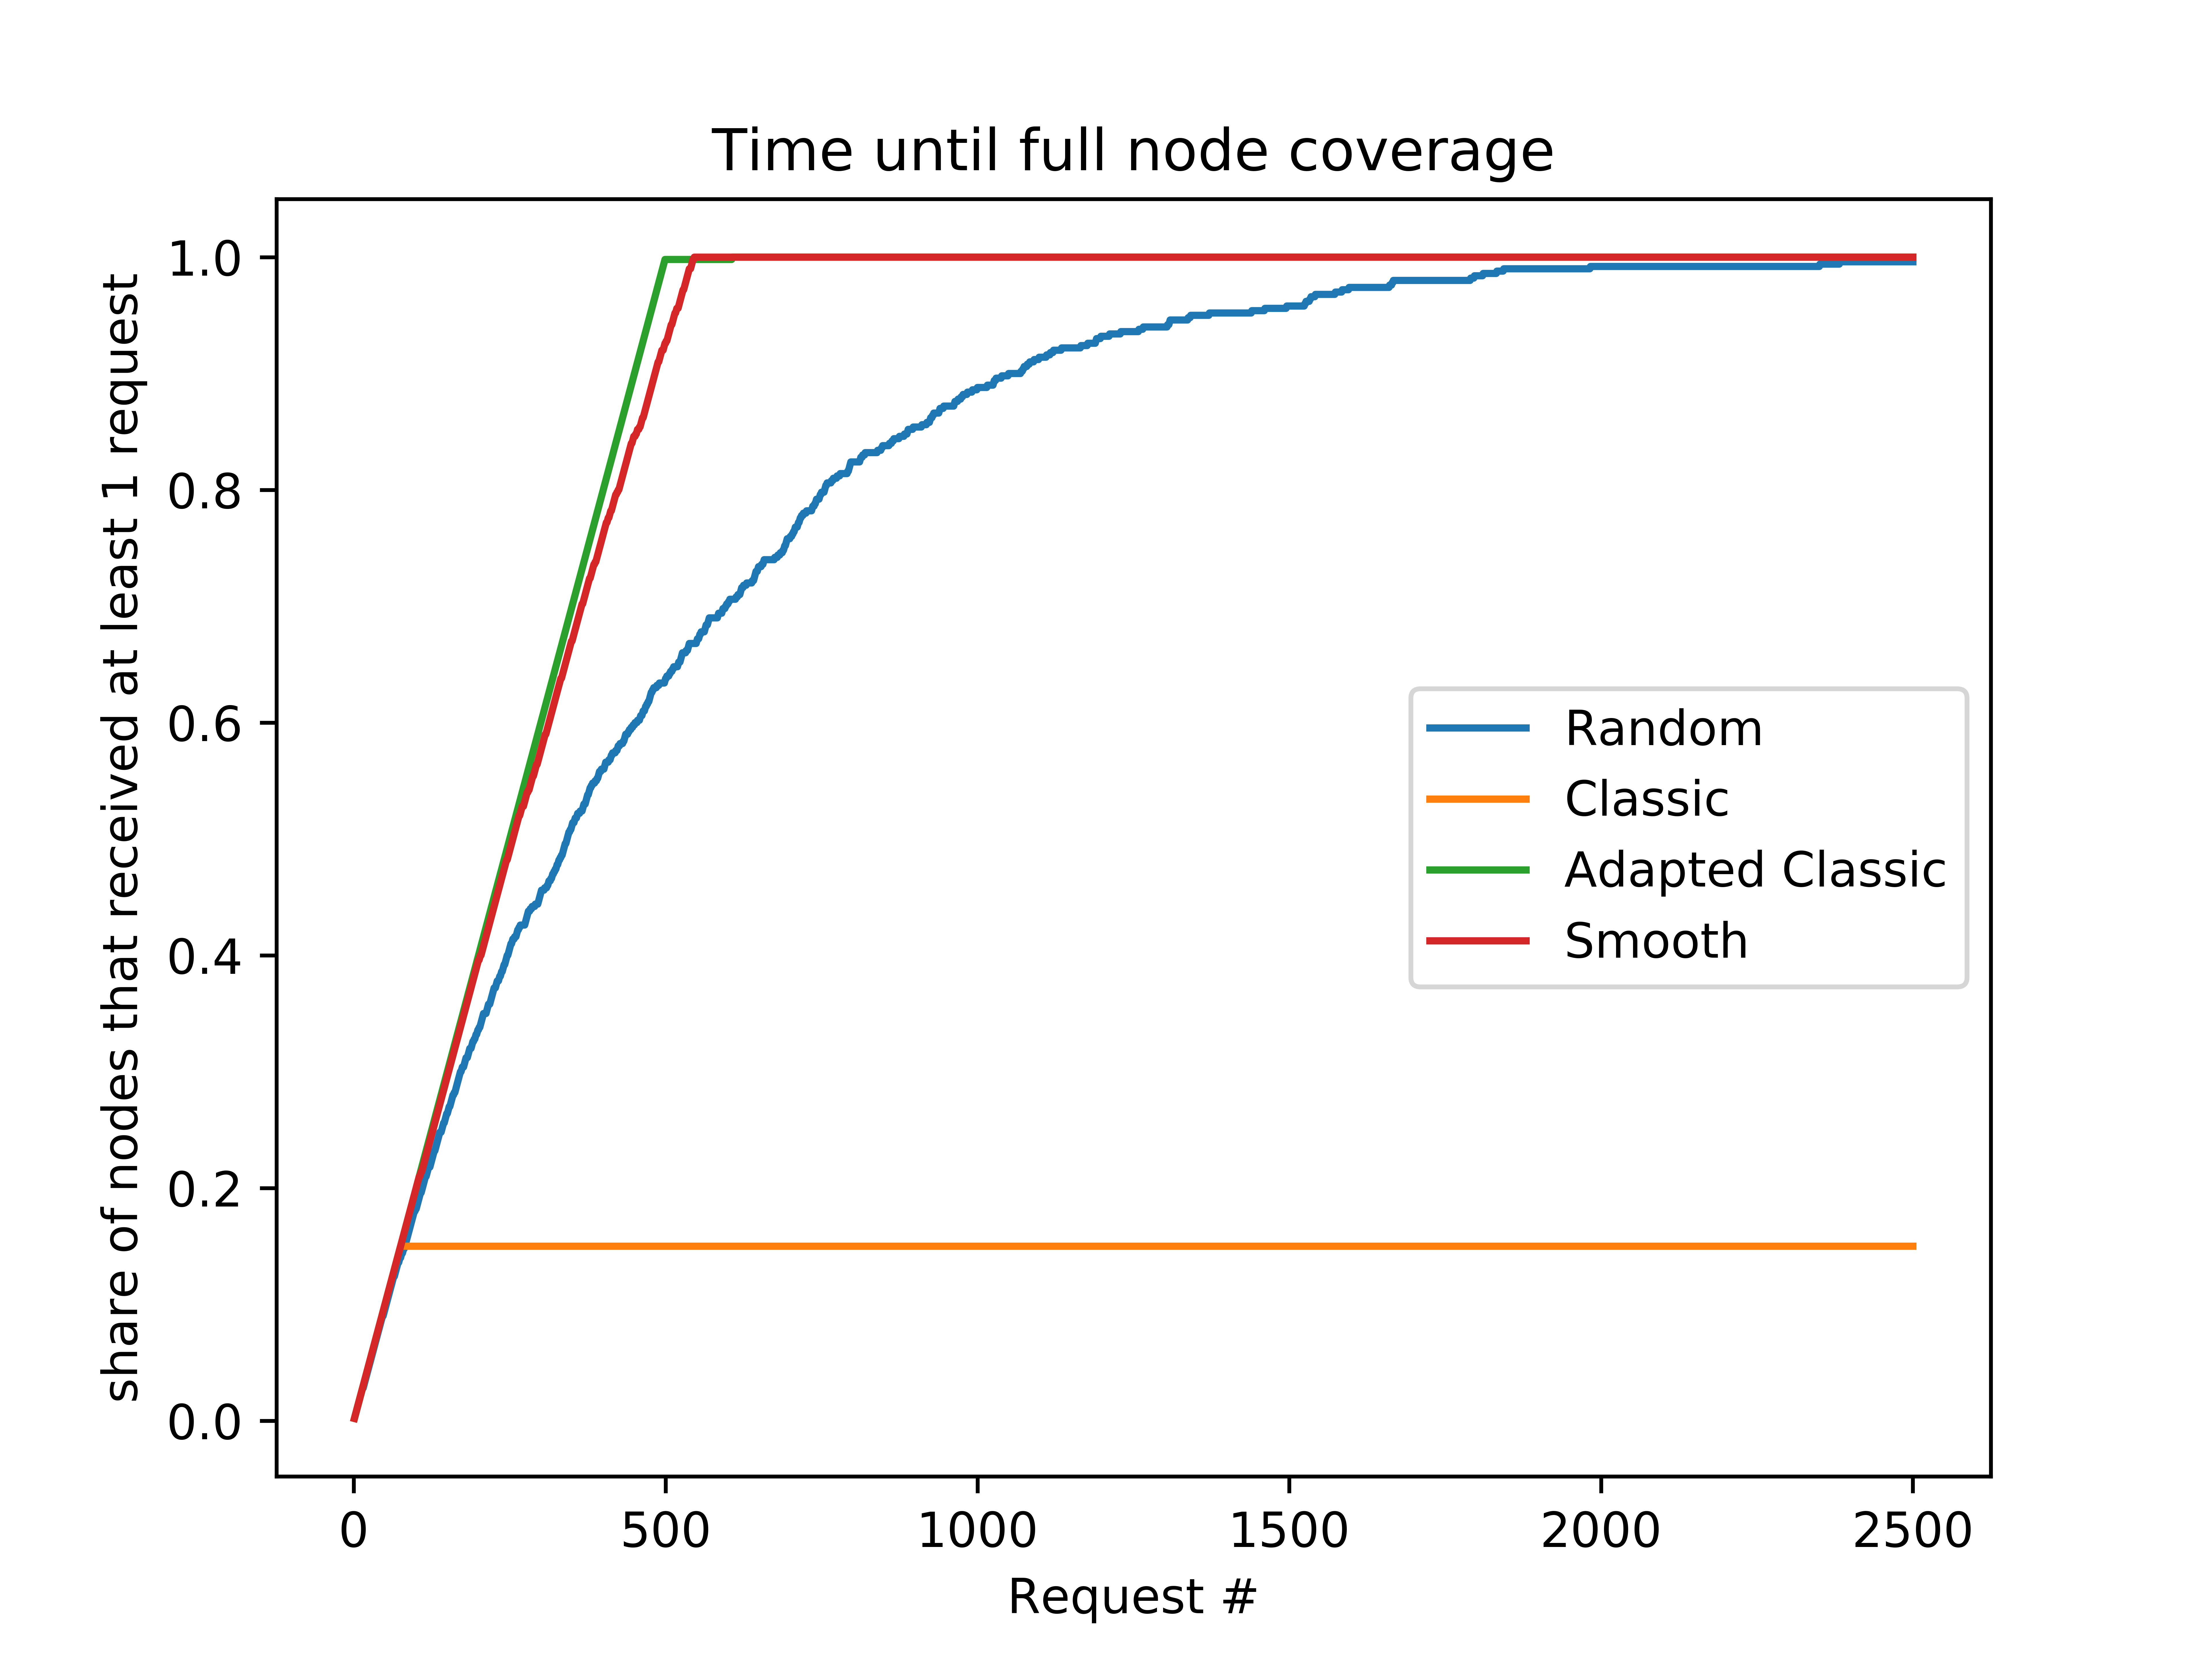
\includegraphics[width=11cm]{graphics/graphs/lb_imp_upstream_coverage.png}
    \caption{A graph showing how quickly each upstream receives at least one request with different weighted round robin implementations for least response time load balancing}
    \label{fig:lb_imp_upstream_coverage}
\end{figure}

\begin{figure}
    \centering
    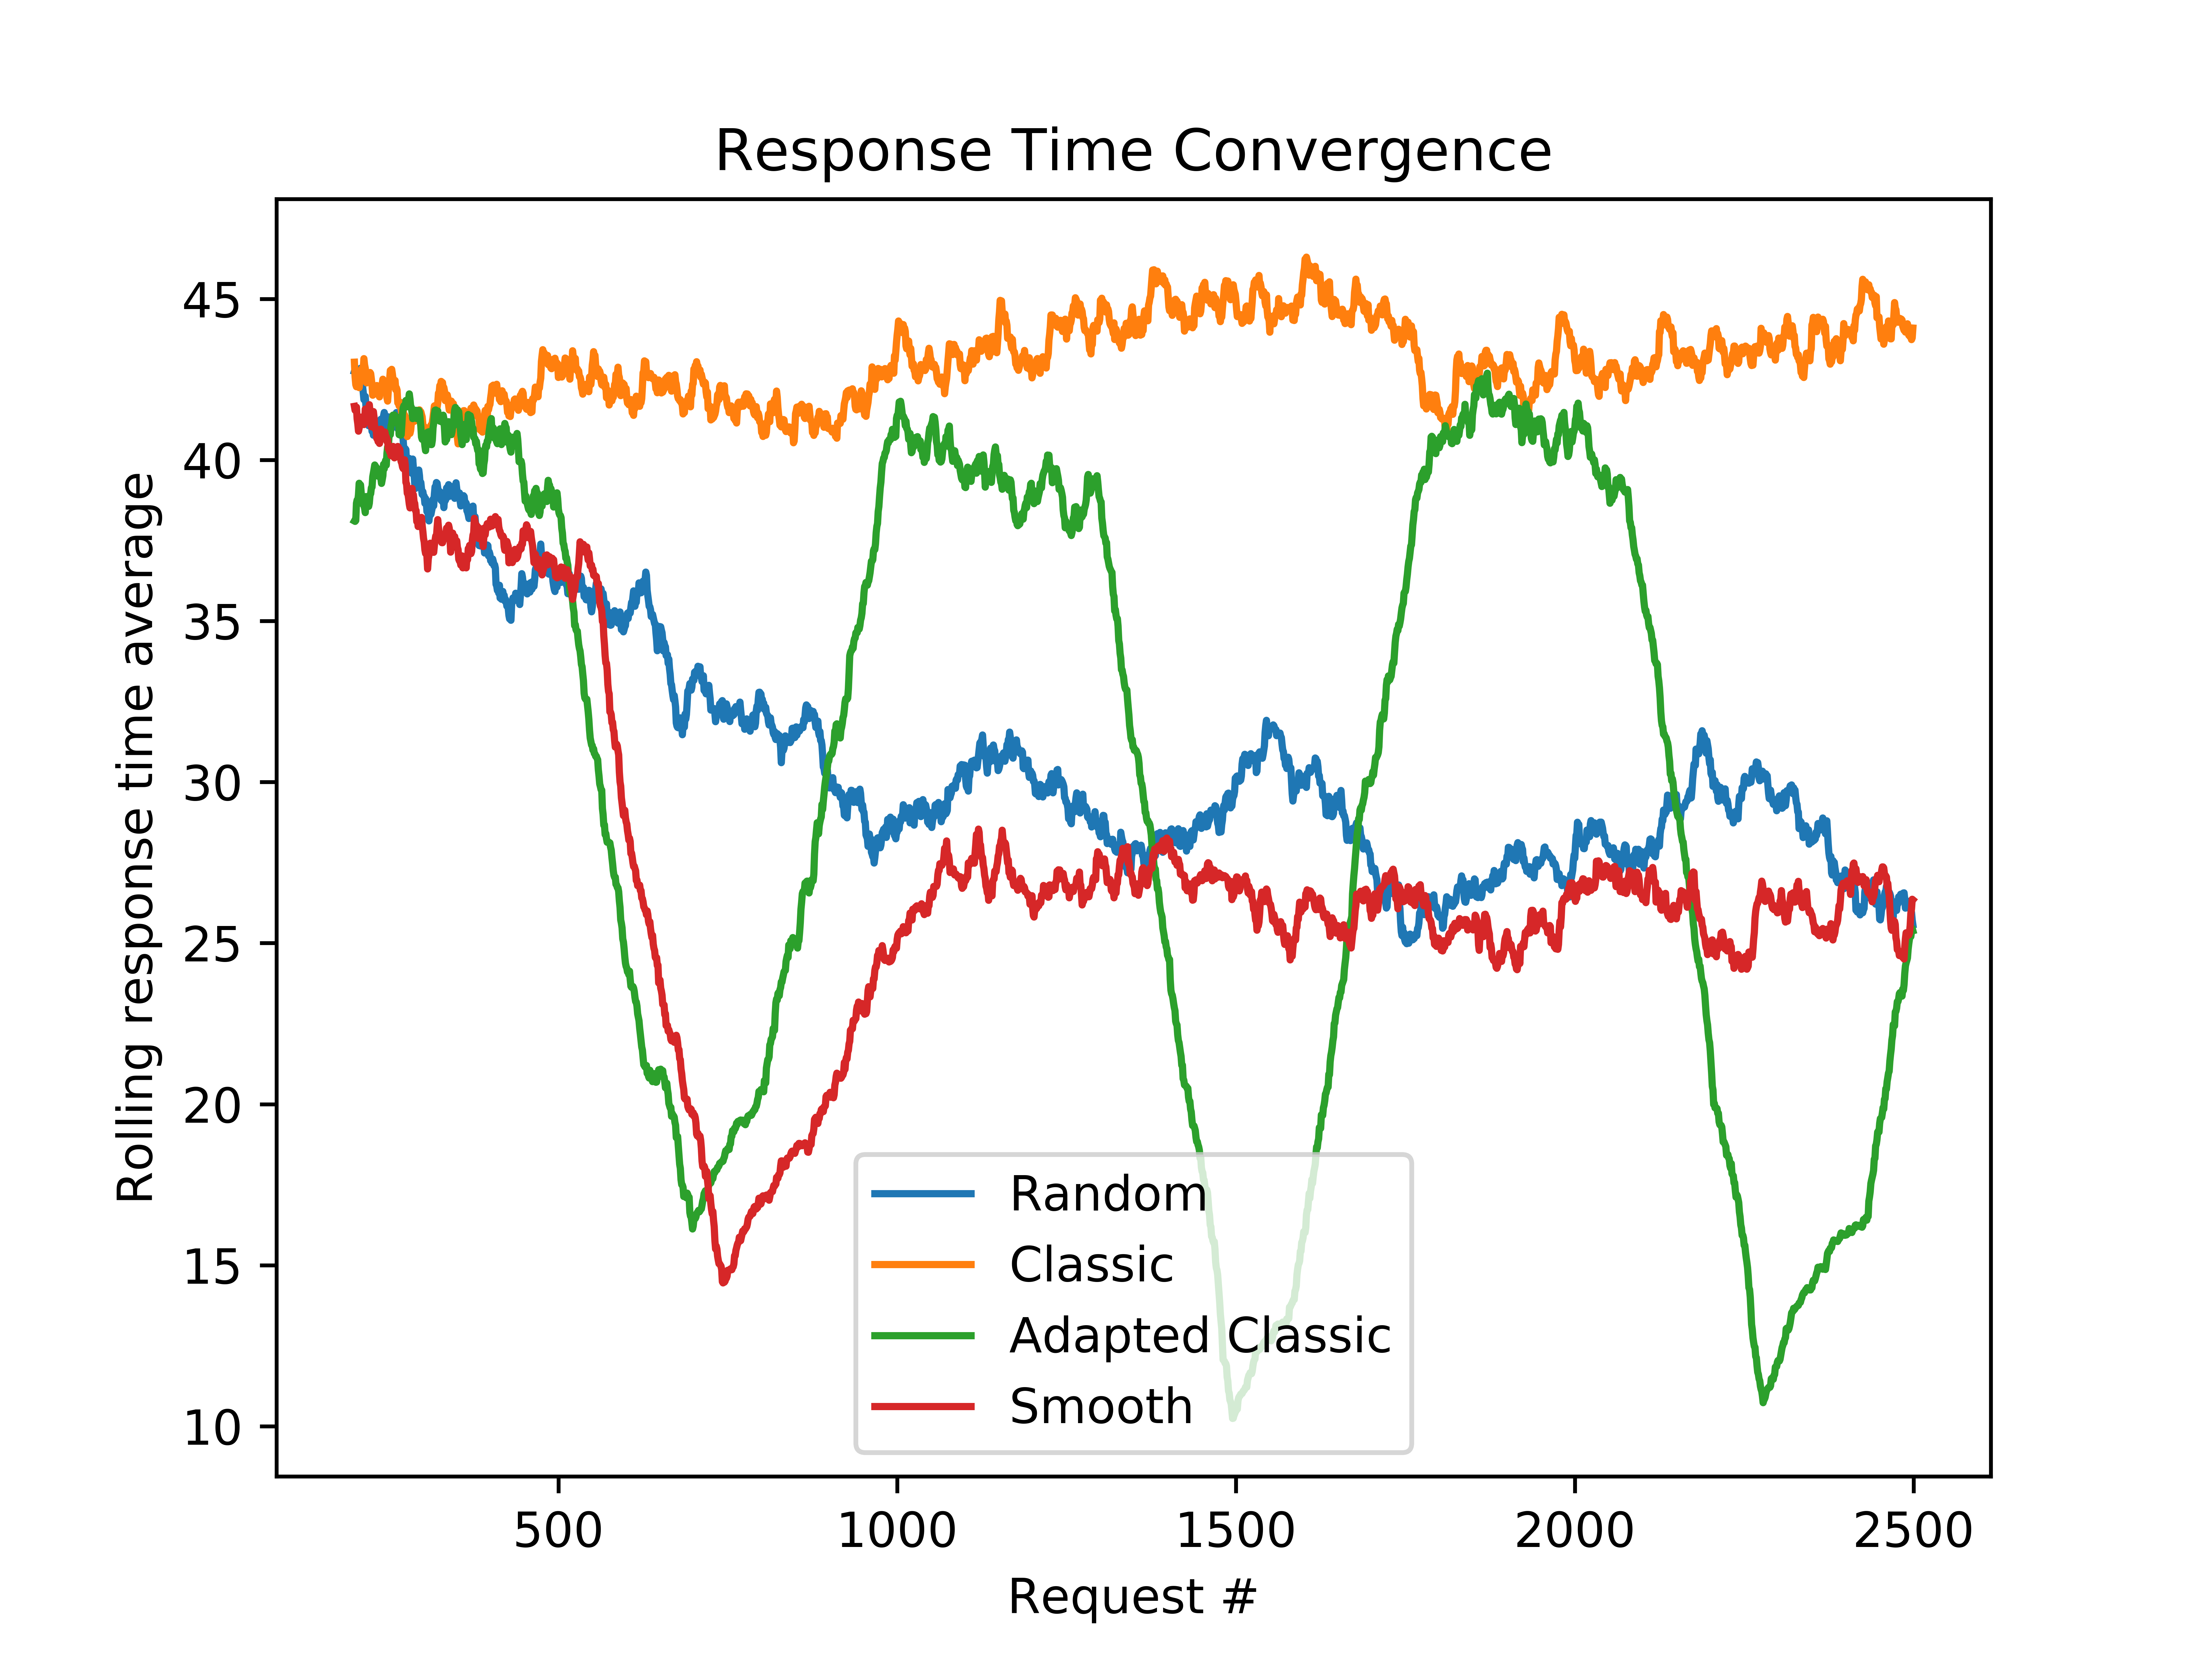
\includegraphics[width=11cm]{graphics/graphs/lb_imp_trt_convergence.png}
    \caption{Graph showing average response times converging for different weighted round robin implementations with least response time load balancing}
    \label{fig:lb_imp_rt_convergence}
\end{figure}

In our results we can see significant differences between the implementations.
First, as can be seen in Figure \ref{fig:lb_imp_upstream_coverage}, there are significant differences on how fast, or whether at all, every node in the system receives at least one request.
Since least response time load balancing relies on requests to evaluate the performance of an upstream, the quality of the solution is limited by the amount of information available about the upstreams.
We can see that the classic implementation never sends requests to more than a small subset of upstreams, which is due to its internal state being reset on weight updates.
While the random sampling eventually converges toward covering all upstreams, both the smooth and adapted classic implementation do so much more quickly.
The adapted classic is even a slight bit faster than the smooth implementation, but from our point of view we consider this difference to be negligible.

We also observe drastically different behaviour of the average response times between the different implementations.
Figure \ref{fig:lb_imp_rt_convergence} shows that Classic never reaches the level of performance of the other implementations, most likely due to it never discovering the faster subset of upstreams.
While we can also observe that for both the smooth and the random reference implementation average response times stabilize eventually, the adapted classic shows an alternating pattern of fast and slow response time averages.
This is due to the implementation, which works through the highest weighted upstreams first, before including the next highest weighted ones and so on.
Since the order in which this happens is deterministic this oscillating performance pattern forms.
The classic implementation shows the same behaviour, but due to it only ever sending requests to a smaller set of upstreams the pattern isn't as easily visible.
Note that as we are considering response time averages low values on the y-axis in Figure \ref{fig:lb_imp_rt_convergence} are desirable.












% for discussion: shows that default implementations don't necessarily fit least response time / edge computing and need to be adapted. Also shows how unintuitive behaviour can be
% can discuss potential performance tradeoffs between spending "resources" on node discovery vs. using already known nodes that work well.














\DIFdelbegin %DIFDELCMD < \newpage 
%DIFDELCMD <  \newpage %%%
\section{\DIFdel{Load Balancer Parametrization}}
%DIFAUXCMD
\addtocounter{section}{-1}%DIFAUXCMD
\DIFdelend \DIFaddbegin \subsection{\DIFadd{Load Balancer Parametrization}}
\DIFaddend % with graphics 2 pages -> with graphics got 5-6 pages.
With this range of experiments we set out to better understand the effects different parameters have on a load balancers performance.
We then continue to use this information to make an informed decision for the load balancer parameters in subsequent experiments.

Specifically, we want to understand the relationship between the following load balancer parameters:
\begin{enumerate}
    \item \textbf{Scaling Factor:} the factor which determines how linearly observed node performance is mapped to weights
    \item \textbf{Weight Range:} the size of the weight range the load balancer can use
    \item \textbf{Current Weight Reset:} whether or not it makes sense to reset the current weights of the load balancers when the weights are changed
\end{enumerate}

\DIFdelbegin \subsection{\DIFdel{Setup}}
%DIFAUXCMD
\addtocounter{subsection}{-1}%DIFAUXCMD
\DIFdelend \DIFaddbegin \subsubsection{\DIFadd{Setup}}
\DIFaddend 

Since previous experiments have shown that the impact parameter changes can have are at times hard to predict, we decided to perform this evaluation using a grid-search, meaning that we rely on trying a large number of permutations to find patterns in their behaviour.
To test these settings we do not rely on the full FaaS-Sim environment, but rather perform isolated tests with a single load balancer and less sophisticated function and network simulations.

Since we are trying to evaluate how well load balancers choose upstreams, the upstreams are the comparatively most accurately simulated component.
The performance model of our simulated upstreams is closely informed by our notion of a node's performance level and capacity, which we outlined in our load balancing approach.
Thus, each simulated upstream has a set level of performance, which determines how long it takes for a request to be processed.
Since our aim is to keep this simulation simple, we consider the response time determined by the upstream to represent both the network and the \gls{fet} that would be observed in a real serverless system.
Each upstream samples its response times from a set of two lognormal distribution, one of which represents the \gls{fet}, while the other represents the network time.
To simulate the effect of high load, each upstream also has a set capacity, measured in requests per second.
If an upstream receives more requests per second than is has capacity for, \glspl{fet} start to degrade linearly, meaning that response times get longer in proportion to how overloaded the upstream is.

To represent different system conditions we introduce \textit{performance spread} as an input variable to these experiments that determines the how heterogeneous the performance of the simulated upstreams is.
The assumed system scenario is closely aligned with the one of our initial evaluation.
Relative to the load balancer a node can fall into one of four location categories, which determine the network distance from the load balancer: \textit{local}, \textit{city}, \textit{nation}, and \textit{global}.
Like it would  be in a real scenario, the probabilities of nodes falling into each of the categories gets progressively higher, meaning that a very low number of nodes will be local, while the majority will be \textit{global} and thus rather far away form a network perspective.
Apart from their location, nodes can fall into three performance categories, which are \textit{small}, \textit{medium}, and \textit{large}.
This performance category determines both the typical \gls{fet} of that node and its capacity.
Small and medium nodes are more likely to be located close to the load balancer, while large nodes are likely to be farther away in the network.
This is done to represent a typical edge computing scenario where relatively weaker compute is available locally, with a large amount available farther away, e.g. in the cloud.
The performance spread then determines how big the differences between the different categories nodes can fall into are.
A performance spread of 15 for example would correspond to as scenario where \glspl{fet} range from 10ms to 150ms, capacities from 5\gls{rps} to 100\gls{rps}, and network times from 5ms to 250ms.
A higher performance spread would indicate higher performance differences, while a lower one would indicate lower differences, with a performance spread of 1 indicating complete homogeneity.


To make an informed decision on load balancer parametrization we performed three experiments.
\subsubsection{Scaling Factor and Performance Spread}
In this evaluation we examine the effect the scaling factor has on performance in a variety of different scenarios.
To this end we tested scaling factors from 0,1 to 10.
Scenarios included performance spreads from 1 to 46, and all scenarios were repeated three times with request loads of 50\gls{rps}, 250\gls{rps}, and 1000\gls{rps}.
The weight range upstreams were mapped onto in this experiment is [1;10].
The experiment covers a simulated time frame of 1000 seconds.

\begin{figure}
    \centering
    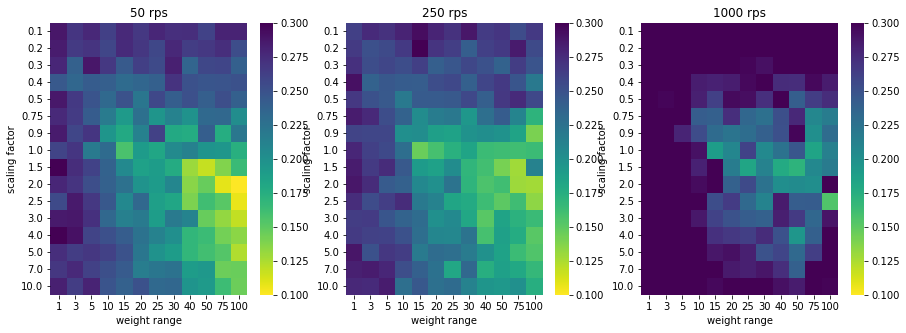
\includegraphics[width=14cm]{graphics/graphs/lb_hyper_scaling_vs_performance_spread.png}
    \caption{Mean response time over various levels of performance spread and scaling factors}
    \label{fig:lb_hyper_scaling_perfspread}
\end{figure}

The results of this experiment can be seen in Figure \ref{fig:lb_hyper_scaling_perfspread}.
Aside from showing lower performance for higher performance spreads, which is entirely to be expected since a larger performance spread means nodes are farther away and have higher \glspl{fet}, there are no significant differences between the scaling factors.

\subsubsection{Scaling Factor and Weight Range}
Analogously, we also evaluated the relationship between the scaling factor and weight range using a grid-search type experiment.
We once again tested scaling factors in the range [0,1;10] with request loads of 50\gls{rps}, 250\gls{rps}, and 1000\gls{rps}.
For the weight range the minimum weight was always set to 1, and the max weight between 1 and 100.
The performance spread was fixed over all experiments at 15, and the simulation is again run for 1000 seconds.

\begin{figure}
    \centering
    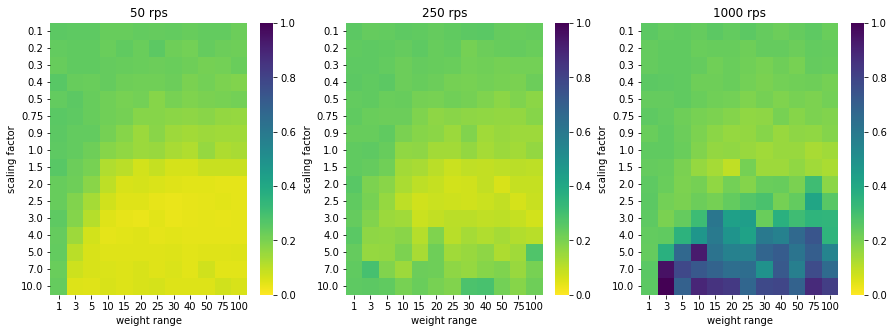
\includegraphics[width=14cm]{graphics/graphs/lb_hyper_scaling_vs_weight_range.png}
    \caption{Mean response time over different weight ranges and scaling factors}
    \label{fig:lb_hyper_weightrange_scaling}
\end{figure}

The results of this evaluation can be seen in Figure \ref{fig:lb_hyper_weightrange_scaling}.
Results show a clear trend towards higher weight ranges and scaling factors that are close to or slightly above 1, which would correspond to linear scaling.
We can also observe that higher request loads lead to worse performance on average, as one would expect, and also seem to shrink the set of configurations that provide good performance.

\subsubsection{Resetting Weights on Updates and Weight Update Intervals}
Our implementation of weighted round robin described earlier has a set of two weights for each upstream: the weight, and the current weight.
Once the weight of an upstream changes, we can choose to also reset the current weight or leave it as is.
Since intuitively there was no clear answer as to which choice is better, and the testing infrastructure around this was already in place, we chose to perform an experiment to measure the impact of this choice.
Apart from whether or not weights should be reset on updates, one also needs to decide at which interval weight updates should occur.
To evaluate this choice we performed these experiments using a variety of different update intervals.
Since we expected that resetting weights will have an outsized effect for scenarios with a low request rate, we performed experiments over a wider range of request loads than before, and also tested over different weight ranges.
Request load ranges from 2\gls{rps} to 1000\gls{rps}, weight update frequency from 5 seconds to 200 seconds, and maximum weight once again from 1 to 100.
Lastly, all experiments simulated a timeframe of 1000 seconds.

\begin{figure}
    \centering
    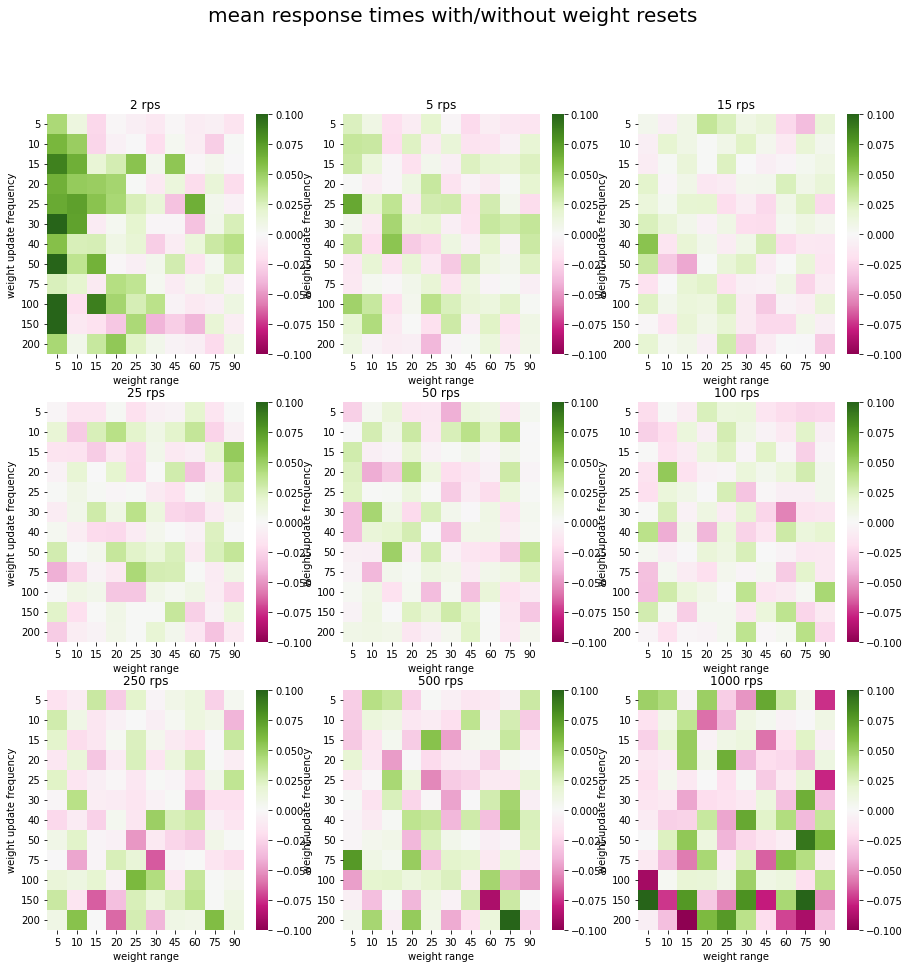
\includegraphics[width=14cm]{graphics/graphs/lb_hyper_weight_reset_delta.png}
    \caption{Difference between resetting and not resetting weights on update. Positive values indicate not resetting performs better, while negative values indicate the opposite.}
    \label{fig:lb_hyper_reset_delta}
\end{figure}

\begin{figure}
    \centering
    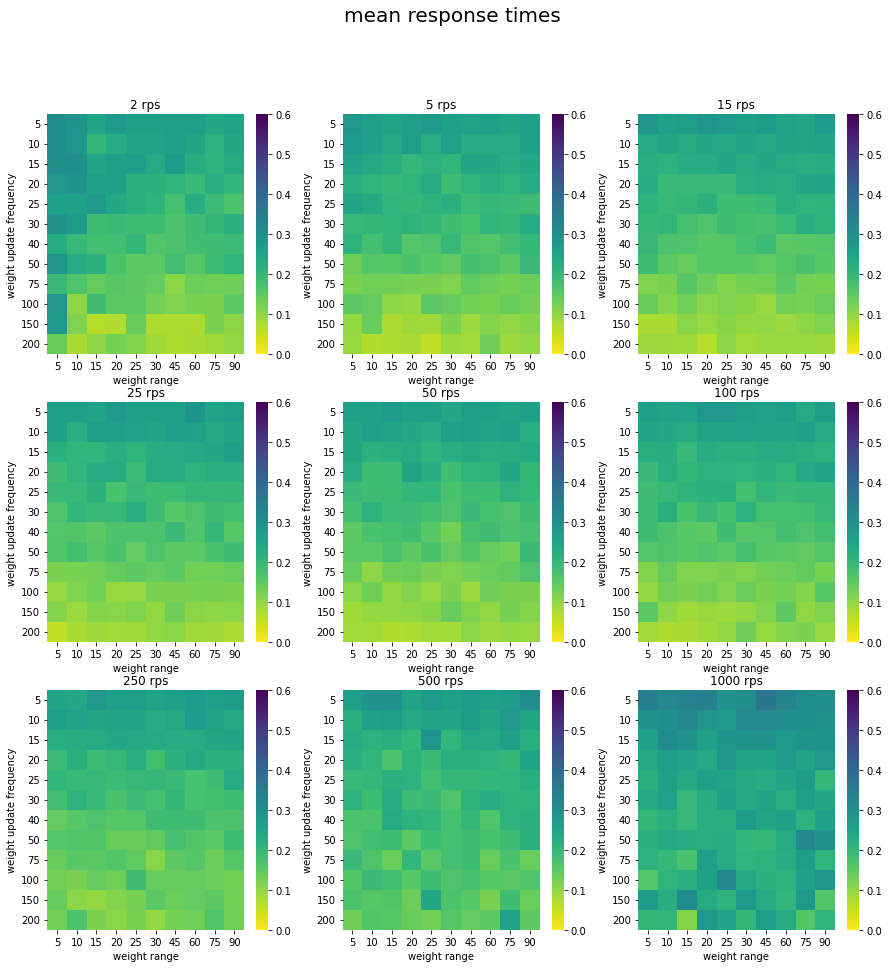
\includegraphics[width=14cm]{graphics/graphs/lb_hyper_mean_with_reset.png}
    \caption{Mean response times over different weight ranges and weight update times. Current weights are reset on update.}
    \label{fig:lb_hyper_reset_mean}
\end{figure}

\begin{figure}
    \centering
    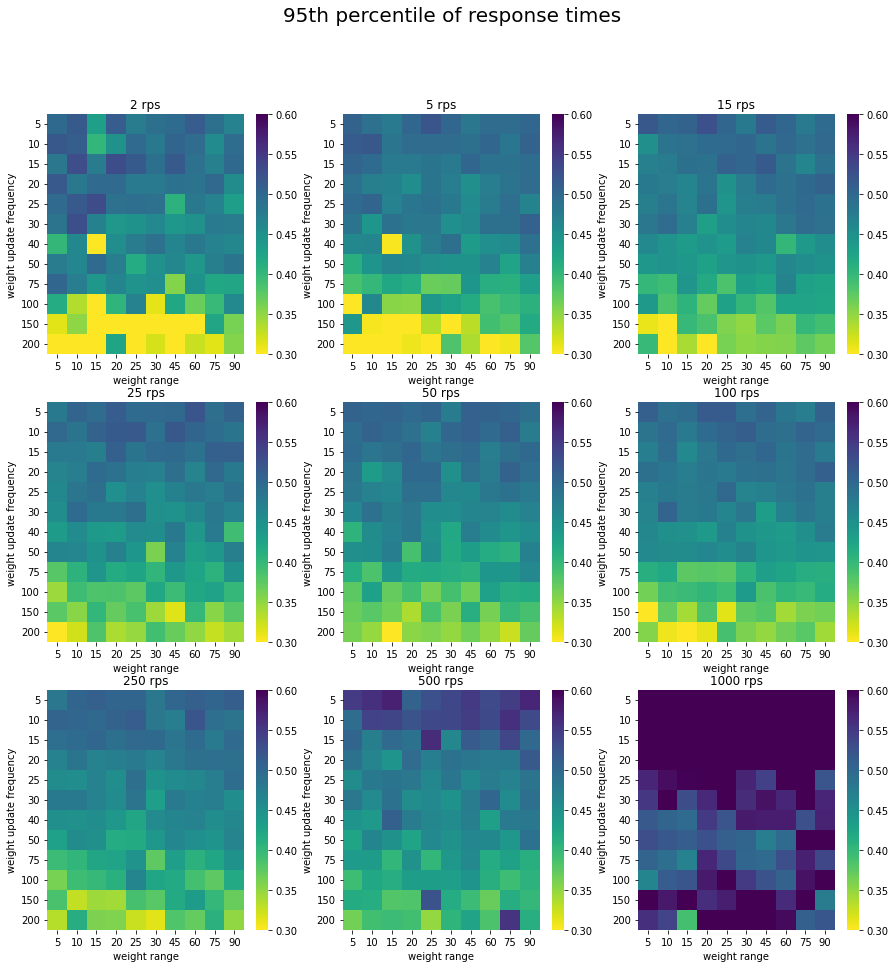
\includegraphics[width=14cm]{graphics/graphs/lb_hyper_95th_percentile_with_reset.png}
    \caption{95th percentile of response times over different weight ranges and update times. Current weights are reset on update.}
    \label{fig:lb_hyper_reset_q95}
\end{figure}

Figure \ref{fig:lb_hyper_reset_delta} shows the difference between the mean values of resetting or not resetting current weights.
In the results there is no clear indication resetting or not resetting is clearly superior.
There is a slight trend for not resetting performing better with low request rates, and resetting leading to better results in very high \gls{rps} scenarios.

Figure \ref{fig:lb_hyper_reset_mean} shows a trend towards longer intervals for weight updates performing better, irrespective of the weight range.
Figure \ref{fig:lb_hyper_reset_q95}, which shows the 95th percentile of the same data generally indicates the same tendency, although not for all request levels.
While at low request rates long update intervals perform better, they perform worse than shorter update intervals for high request rates.
Lastly we advise that care should be taken when comparing these visualizations, as the scale sometimes differs.
This is always indicated on the side of the visualization, and was necessary to better show relative differences within the same experiment run.


% Notes for discussion:
% QoS issue where one setting might be good under certain conditions, but bad under others e.g. 95th percentile type stuff
% extremes seem not to do so well for the most part
% behavious is to a large degree as expected: for low RPS super steep scaling works fine, but it becomes less good once capacity of the best nodes is reached
% No super clear point for or against weight resetting, once again depends on situation -> this points to a further investigation of the role of node discovery.
% to a degree weight resets perform a bit as expected in that low rps strongly prefer not resetting, and high rps preferring resets
%DIF <  explanation why is quite intuitive, especially w.r.t.  \newpage 
 \DIFdelbegin %DIFDELCMD < \newpage %%%
\DIFdelend %DIF >  explanation why is quite intuitive, especially w.r.t. 
\DIFaddbegin 

\DIFaddend \section{\DIFdelbegin \DIFdel{Load Balancer }\DIFdelend Resource Usage \DIFaddbegin \DIFadd{and Load Balancer Scale}\DIFaddend }
\subsection{\DIFaddbegin \DIFadd{Load Balancer }\DIFaddend Resource \DIFdelbegin \DIFdel{Evaluation Setup}\DIFdelend \DIFaddbegin \DIFadd{Usage}\DIFaddend }
\DIFaddbegin \subsubsection{\DIFadd{Resource Evaluation Setup}}
\DIFaddend % 2 pages -> got 4
The goal of these experiments is to understand the resource consumption one can expect from a load balancer in the context of serverless edge computing.
Using the traces of these experiments we implement the load balancers within the serverless simulator as close to reality as possible, thus making sure the simulation results are more representative.

As described we use a Kubernetes cluster with a number of different nodes to make real-life measurements of load balancer's performance characteristics, requests are sent via galileo\cite{galileo-github}\cite{operating-energy-aware-galileo}, and the system metrics are measured via telemd\cite{telemd-github}.
Since the load balancer is containerized, just like it would be in a serverless framework, telemd relies on the metrics provided by Kubernetes to measure resource consumption.
Specifically, telemd reports the values provided by the following files at a set interval\cite{telemd-github}.
\begin{lstlisting}[language=Bash]
/sys/fs/cgroup/cpuacct/kubepods/besteffort/pod<pod ID>/<container ID>/cpuacct.usage
/sys/fs/cgroup/memory/kubepods/besteffort/pod<pod ID>/<container ID>/memory.stat
\end{lstlisting}
Network characteristics are not taken into account with these measurements, as they are highly application specific and experimental evaluation is thus neither fruitful nor necessary.

Since scaling and scheduling are important aspects of our approach, we also consider the image size of the load balancer to be relevant.
Because Docker Hub is one of the largest hosting platforms for application container images, we use the information it provides\cite{traefik-dockerhub} to determine the image size for different platforms.

To cover a wide range of possible deployment scenarios the nodes we use for this experiment cover hardware from powerful desktop processors as they are used in large scale data centers to small scale reduced instruction set processors as one finds in mobile devices.

\begin{table}[]
\begin{tabular}{lllll}
\hline
\textbf{Node} & \textbf{\begin{tabular}[c]{@{}l@{}}Processor\\ Architecture\end{tabular}} & \textbf{\begin{tabular}[c]{@{}l@{}}logical CPU\\ core count\end{tabular}} & \textbf{\begin{tabular}[c]{@{}l@{}}RAM\\ (GiB)\end{tabular}} & \textbf{Model Name}           \\ \hline
AMD           & x86/amd64                                                                 & 8                                                                         & 32                                                           & AMD Ryzen Embedded V1605B     \\
Intel         & x86/amd64                                                                 & 8                                                                         & 16                                                           & Intel Xeon E3-1230 v6         \\
Jetson        & aarch64                                                                   & 4                                                                         & 4                                                            & NVIDIA Jetson Nano            \\
RockPi        & aarch64                                                                   & 6                                                                         & 4                                                            & RockPi 4B                     \\
RPi           & ARMv7                                                                     & 4                                                                         & 1                                                            & Raspberry Pi 4Model B Rev 1.1
\end{tabular}
\caption{Nodes present in the real Kubernetes cluster used for resource consumption evaluation}
\label{tab:k8s_nodes}
\end{table}



Table \ref{tab:k8s_nodes} shows the different nodes that are present in the cluster and which get evaluated. Aside from covering typical compute resources we also include a number of ARM devices, one with special purpose compute acceleration, to show how mobile edge computing devices or devices built for purposes such as image processing would perform.

To evaluate load balancer's resource consumption we need to select a real load balancer implementation that serves as a stand-in for generic load balancers.
For this purpose we selected traefik proxy\cite{traefik}, a level 7 load balancer and application proxy.
We considered it a fitting example of a real world load balancer since it is available on all the different platforms we want to test, supports the kind of complex load balancing required of our proposed approach.
It is also open source, which allowed us to extend it with least response time load balancing capabilities like we proposed, which further moves these experiments closer to real-world conditions.
This modified version\cite{traefik-jjnp} is also open source and is already functional, although it does not feature the integrations that would allow its use in a serverless framework.

Since in the experimental setup requires actual requests being sent we also need an upstream the load balancer can then forward the requests it receives to.
For this experiment the upstream is a separate application that does nothing but respond to the requests with a given payload.
Its only distinguishing feature is that we can choose from a random distribution that determines how long the application waits before responding, thus simulating the \gls{fet} usually experienced within a serverless system.
For the general evaluation of different devices we simulated a response time/\gls{fet} of 20 milliseconds.
We built this application specifically for this purpose, and also made it publicly available\cite{palecekResponder2021} so that it can be used by others.
We oriented our payload on a hypothetical edge intelligence application, where a client sends an image for it to then be classified.
Our payload is thus a compressed JPEG image with a file size of 250KiB, while the response is a simple JSON with negligible size.

Lastly for the request load we decided to test a range of different loads.
To do this in a simple and presentable way we send requests along a pattern, which steadily increases the amount of requests sent from 0 to 250 requests per second over a period of 300 seconds, then continuously sending 250 requests per second for 60 more seconds before stopping completely.

Apart from the evaluation of different types of devices we performed another test with the same request pattern, but one time with the previously used response time of 20ms and once again with a response time of 250ms to see whether the response time of the upstreams makes a difference to the load balancer resource consumption.
\DIFdelbegin \subsection{\DIFdel{Observed Resource Consumption}}
%DIFAUXCMD
\addtocounter{subsection}{-1}%DIFAUXCMD
\DIFdelend \DIFaddbegin \subsubsection{\DIFadd{Observed Resource Consumption}}
\DIFaddend Our results show that the resource consumption of load balancers of this class is, generally speaking, quite moderate.
At a rate of 250 requests per seconds, a substantial load, CPU utilization ranges from 4,3\% to 34\%, while memory consumption is between 12 and 59MiB.
The results at 250 requests per second can be seen in Table \ref{tab:resource_eval_results}.

The relationship between the resource consumption and request load can be seen in Figure \ref{fig:lb_resources_by_type}.
From these graphs we can see that CPU utilization rises almost linearly with the number of concurrent requests, while the RAM consumption does not show a comparable pattern.
In fact, the memory consumption shows significant variance between the different nodes with some nodes showing more than quadruple the system memory usage of others.
There is also no obvious explanatory pattern to be observed, as these wide ranges of memory consumption also exist within nodes of the same processor architecture.

The response time of the upstream services also appears to influence resource utilization as can be seen in Figure \ref{fig:lb_resources_by_rt}.
While the CPU utilization seems to be consistent throughout the experiments with 20ms and 250ms response time, the memory consumption is higher for the case of 250ms.

Lastly, the size of the different Docker images, which can be seen in Table \ref{tab:resource_eval_results}, does differ across processor architectures, but not to a significant degree.
The difference between the largest and the smallest images is 2,28Mib, or 8\% to 8,5\%, depending on which image is considered the default basis for the calculation.


\begin{table}[]
\begin{tabular}{lrrr}
\hline
\textbf{Node} & \textbf{CPU utilization} & \textbf{RAM Usage} & \textbf{Docker Image Size} \\ \hline
AMD           & 4,3\%                    & 57 MiB             & 28.46 MB                   \\
Intel         & 6,5\%                    & 16 MiB             & 28.46 MB                   \\
Jetson Nano   & 12,5\%                   & 16 MiB             & 26.18 MB                   \\
RockPi        & 13\%                     & 59 MiB             & 26.18 MB                   \\
RPi           & 34\%                     & 12 MiB             & 26.75 MB                  
\end{tabular}
\caption{Results of the load balancer resource evaluation at 250 requests per second}
\label{tab:resource_eval_results}
\end{table}
\begin{figure}
    \centering
    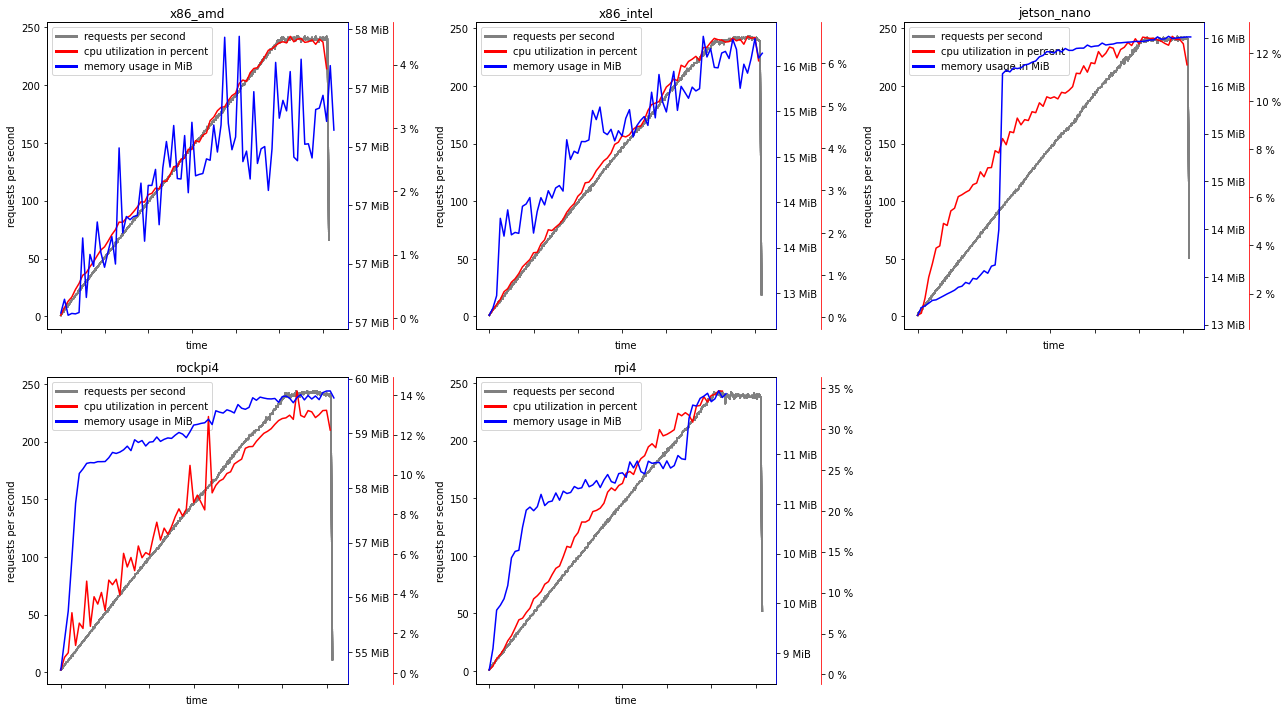
\includegraphics[width=14cm]{graphics/graphs/lb_resources_by_device.png}
    \caption{Resource consumption of the traefik\cite{traefik} load balancer on different devices with a response time of 20ms and request payload size of 250KiB}
    \label{fig:lb_resources_by_type}
\end{figure}

\begin{figure}
    \centering
    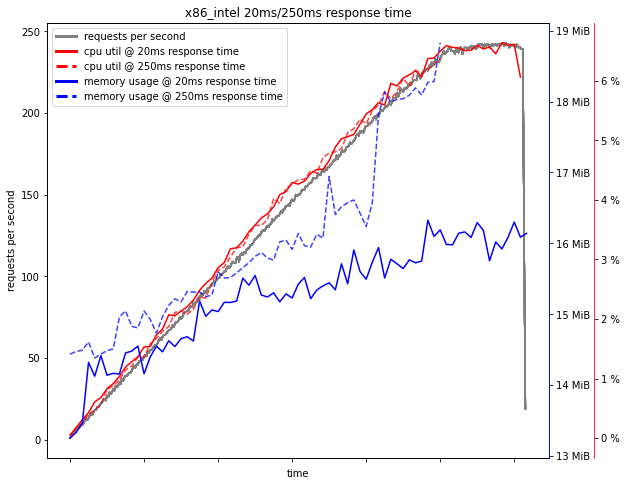
\includegraphics[width=11cm]{graphics/graphs/lb_resources_by_response_time.png}
    \caption{Resource consumption of the traefik\cite{traefik} load balancer with different response times on and a 250KiB request payload}
    \label{fig:lb_resources_by_rt}
\end{figure}
\DIFdelbegin %DIFDELCMD < \newpage 
%DIFDELCMD <  \newpage %%%
\section{\DIFdel{Performance Impact of Load Balancer Scale}}
%DIFAUXCMD
\addtocounter{section}{-1}%DIFAUXCMD
\DIFdelend \DIFaddbegin 

\subsection{\DIFadd{Performance Impact of Load Balancer Scale}}
\DIFaddend % 1 page
With this experiment we evaluate the effect different load balancer scales have on the system.
As we already described the quality and thus resulting end user performance of load balancer decisions only stabilizes after a while, since the load balancer first has to evaluate the available upstreams by sending requests to them.
Because of this, having larger numbers of load balancers present in the system might lead to delayed convergence, and thus suboptimal performance.
Having too few load balancers, on the other hand, might lead to lost performance through overly long routes.

To find out how different scales affect the overall system, we test the system performance with fixed percentages of nodes hosting load balancers.
We test a ranges between 5\% and 100\% of nodes hosting load balancers, which in our scenarios across three cities and 400 nodes means between 20 and 400 load balancer instances.
Scheduling load balancer replicas in these scenarios is still left to the Kubernetes scheduler, which means that the location of the node in the topology is not taken into account.

When testing ratios where less than 5\% of nodes hosted load balancers, we ran into frequent occurrences of the simulation not terminating within a feasible time window.
Upon investigation it turned out that if a load balancer was the only one in the city, or otherwise handled a lot of traffic, but happened to be placed onto a node with very limited bandwidth, the network simulation would take an exceedingly long time.
Requests that did go through took so long, that in real-life it would be considered a failed request by timeout.
We take this as an indication of the inherent problematic of current replica scheduling methods in edge computing, and that the usage of current techniques would simply require an outsized number of load balancers to mitigate the risk of such dysfunctional configurations.

The topologies tested are structurally similar to those of the initial evaluation.
Our two testing scenarios are three cities distributed across the United States, and three cities distributed across the globe.
The cities are identical to the ones from the initial evaluation, and feature identical network latencies between them.
The difference between these and the ones of the initial evaluation is that these feature a different internal topology, which is more closely related to edge intelligence\cite{rauschEdgeIntelligenceConvergence2019} and edge computing in general.
The cities in this evaluation have their compute capabilities, i.e. the cluster nodes, either in the city's local cloud data center, on a smart pole, or next to a cellular base station.
Clients are attached either to smart poles or directly to cellular base stations.
Cellular base stations themselves have a high-speed, high-bandwidth uplink to the wider network and feature a lower bandwidth and higher latency wireless connection to the clients.
These wireless properties depend on whether the cellular tower is LTE or 5G based, as both types are present in our scenario and their network properties are based on real world data\cite{braudMulticarrierMeasurementStudy2019}.
Not all cellular towers have directly attached compute capabilities.
In addition, one of the three cities does not feature a data center.

We simulate the cluster over the course of 2000 seconds, once with 25 \gls{rps}, once with 75\gls{rps}.

\begin{table}[]
\begin{tabular}{lrrrr}
\hline
                                                                             & \multicolumn{4}{c}{mean}                                                                                                                                                                                                                                              \\
\textbf{\begin{tabular}[c]{@{}l@{}}Nodes with\\ Load Balancers\end{tabular}} & \textbf{\begin{tabular}[c]{@{}r@{}}Global\\ 75rps\end{tabular}} & \textbf{\begin{tabular}[c]{@{}r@{}}Global\\ 25rps\end{tabular}} & \textbf{\begin{tabular}[c]{@{}r@{}}Nation\\ 75rps\end{tabular}} & \textbf{\begin{tabular}[c]{@{}r@{}}Nation\\ 25rps\end{tabular}} \\ \hline
\textbf{5\%}                                                                 & 210ms                                                           & 132ms                                                           & 220ms                                                           & 141ms                                                           \\
\textbf{10\%}                                                                & 149ms                                                           & 128ms                                                           & 158ms                                                           & 133ms                                                           \\
\textbf{20\%}                                                                & 134ms                                                           & 127ms                                                           & 147ms                                                           & 128ms                                                           \\
\textbf{30\%}                                                                & 132ms                                                           & 124ms                                                           & 141ms                                                           & 127ms                                                           \\
\textbf{40\%}                                                                & 130ms                                                           & 126ms                                                           & 135ms                                                           & 126ms                                                           \\
\textbf{50\%}                                                                & 128ms                                                           & 125ms                                                           & 134ms                                                           & 125ms                                                           \\
\textbf{60\%}                                                                & 129ms                                                           & 126ms                                                           & 133ms                                                           & 126ms                                                           \\
\textbf{70\%}                                                                & 129ms                                                           & 125ms                                                           & 128ms                                                           & 126ms                                                           \\
\textbf{80\%}                                                                & 128ms                                                           & 128ms                                                           & 131ms                                                           & 125ms                                                           \\
\textbf{90\%}                                                                & 129ms                                                           & 125ms                                                           & 129ms                                                           & 125ms                                                           \\
\textbf{100\%}                                                               & 127ms                                                           & 125ms                                                           & 129ms                                                           & 126ms                                                           \\ \hline
\end{tabular}
\caption{Mean \gls{trt} values of different load balancer scales, once they have converged to a stable value}
\label{tab:lb_scaling_converged_trt}
\end{table}

\begin{figure}
    \centering
    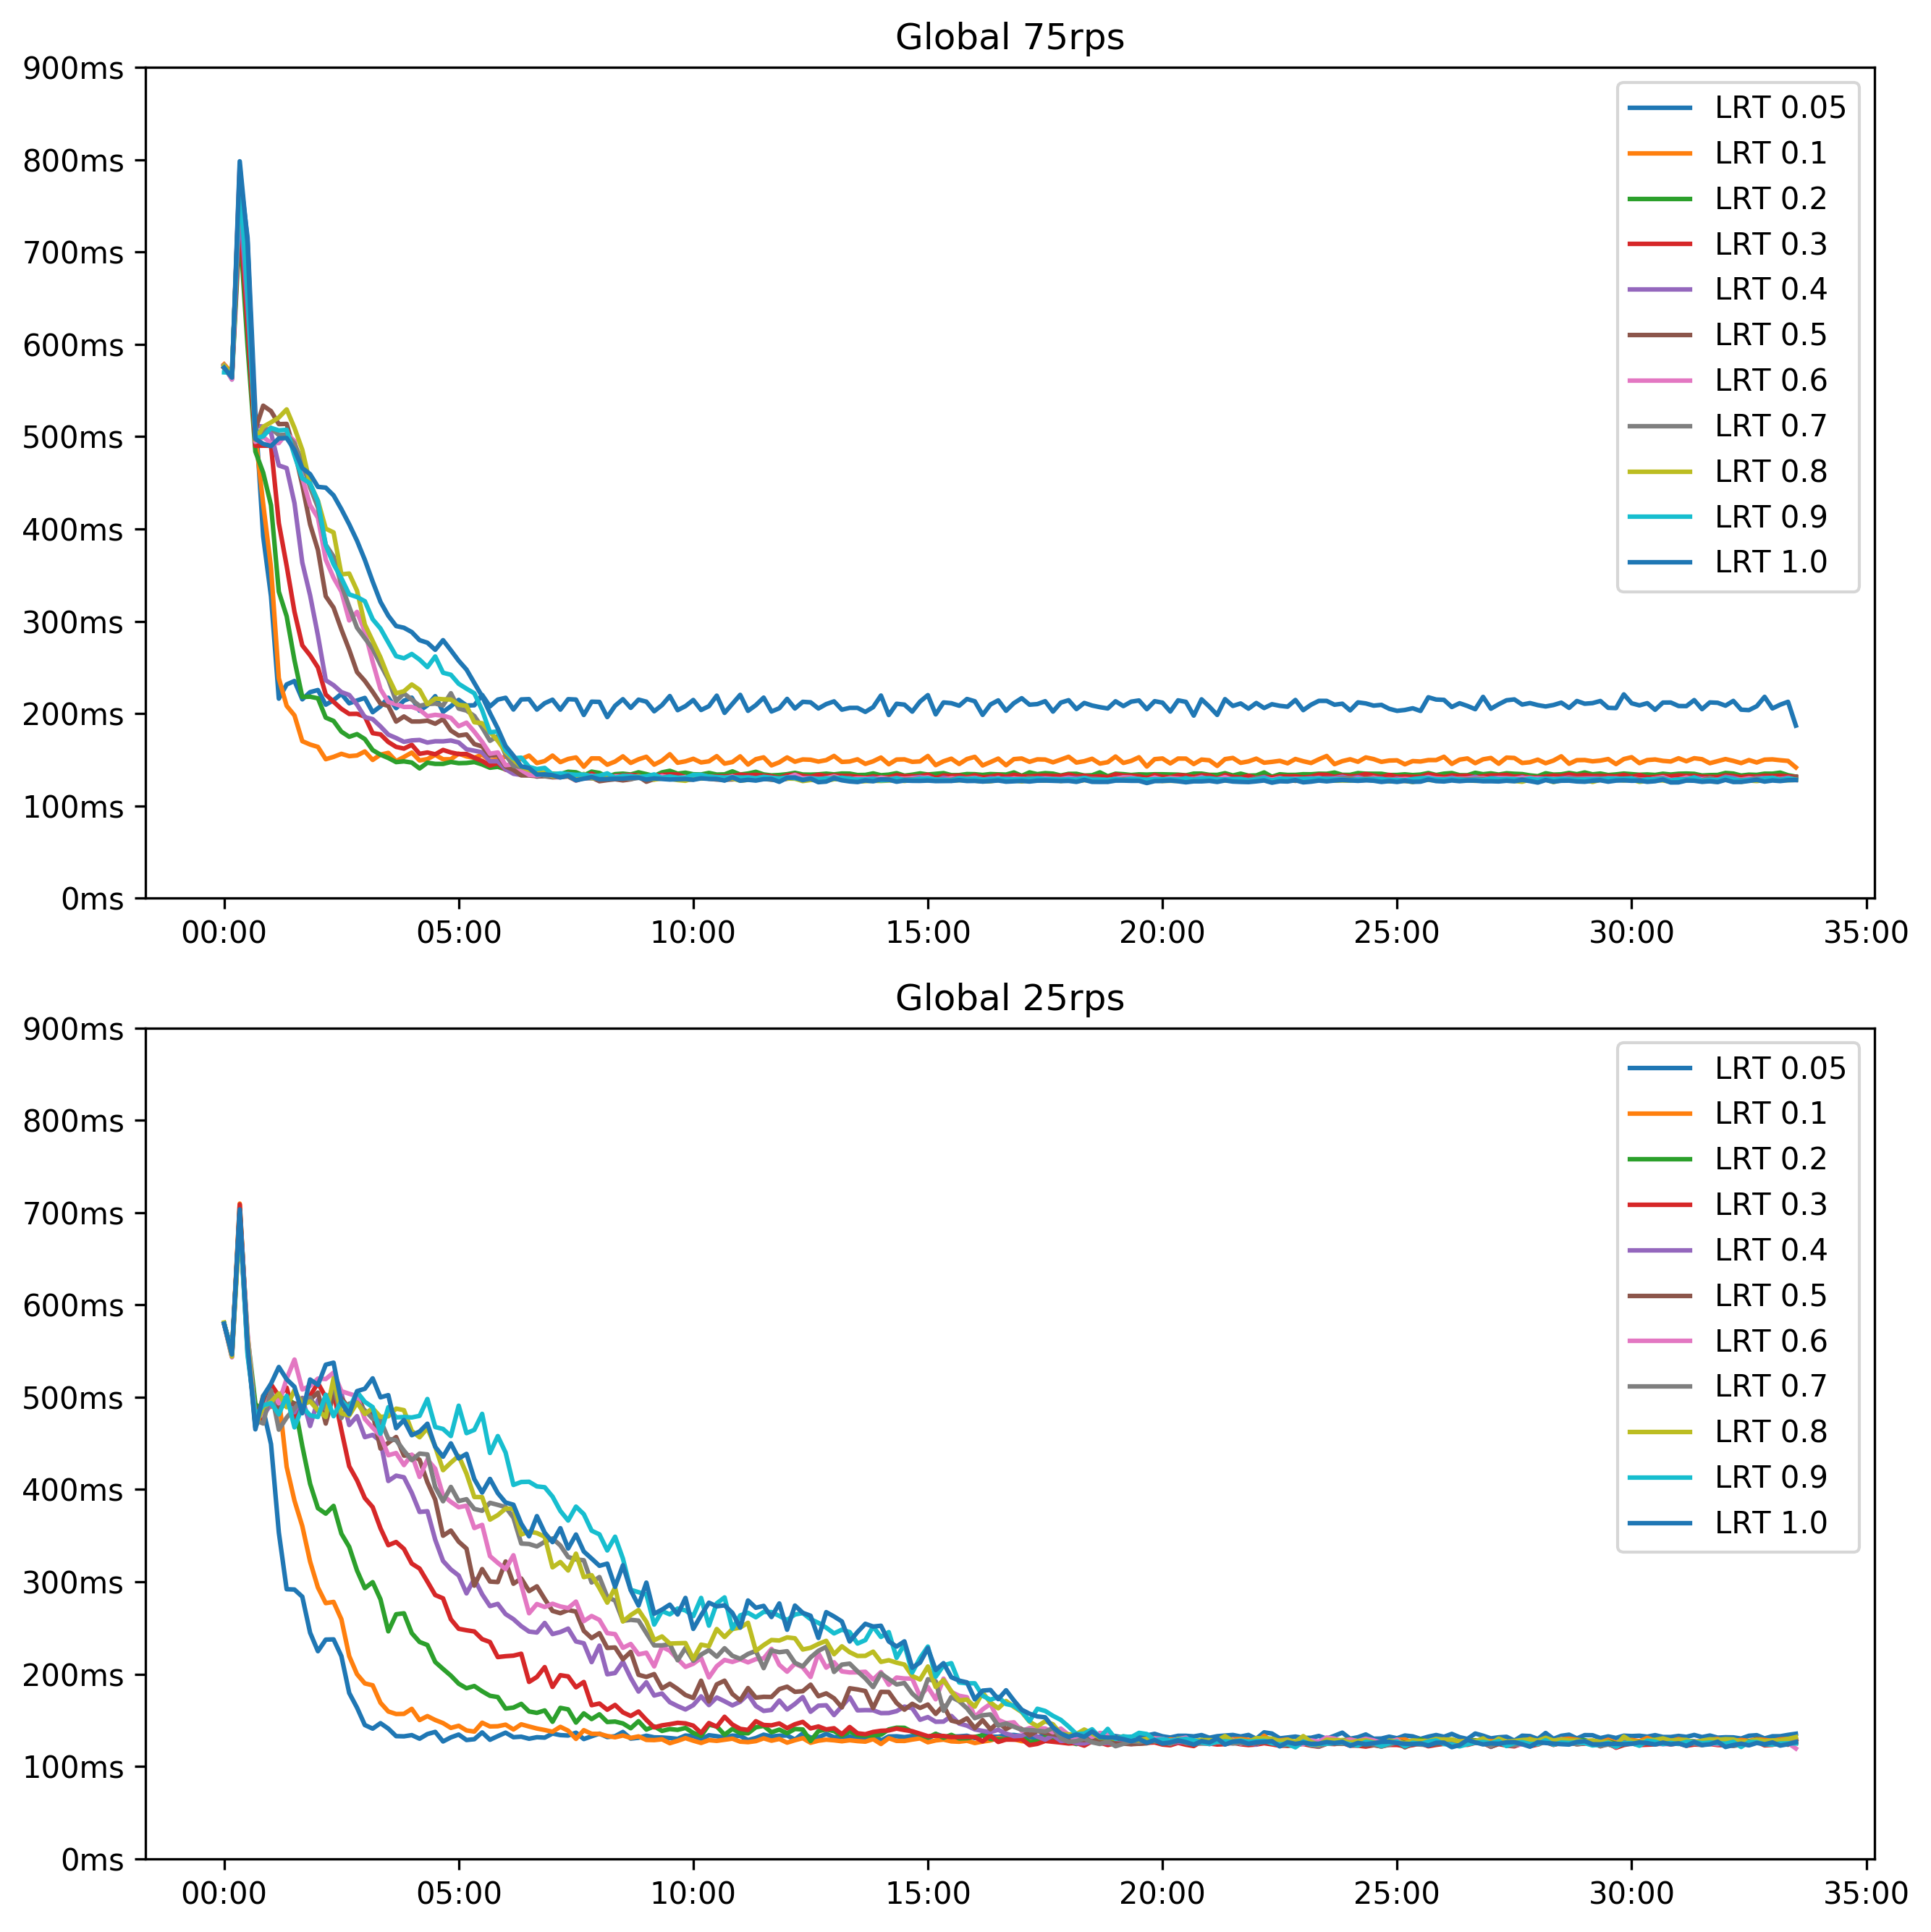
\includegraphics[width=\linewidth]{graphics/graphs/global_lb_scale.png}
    \caption{\glspl{trt} of different load balancer scales in the global scenario. For legibility a 10 second moving average is applied.}
    \label{fig:lb_scale_global}
\end{figure}

\begin{figure}
    \centering
    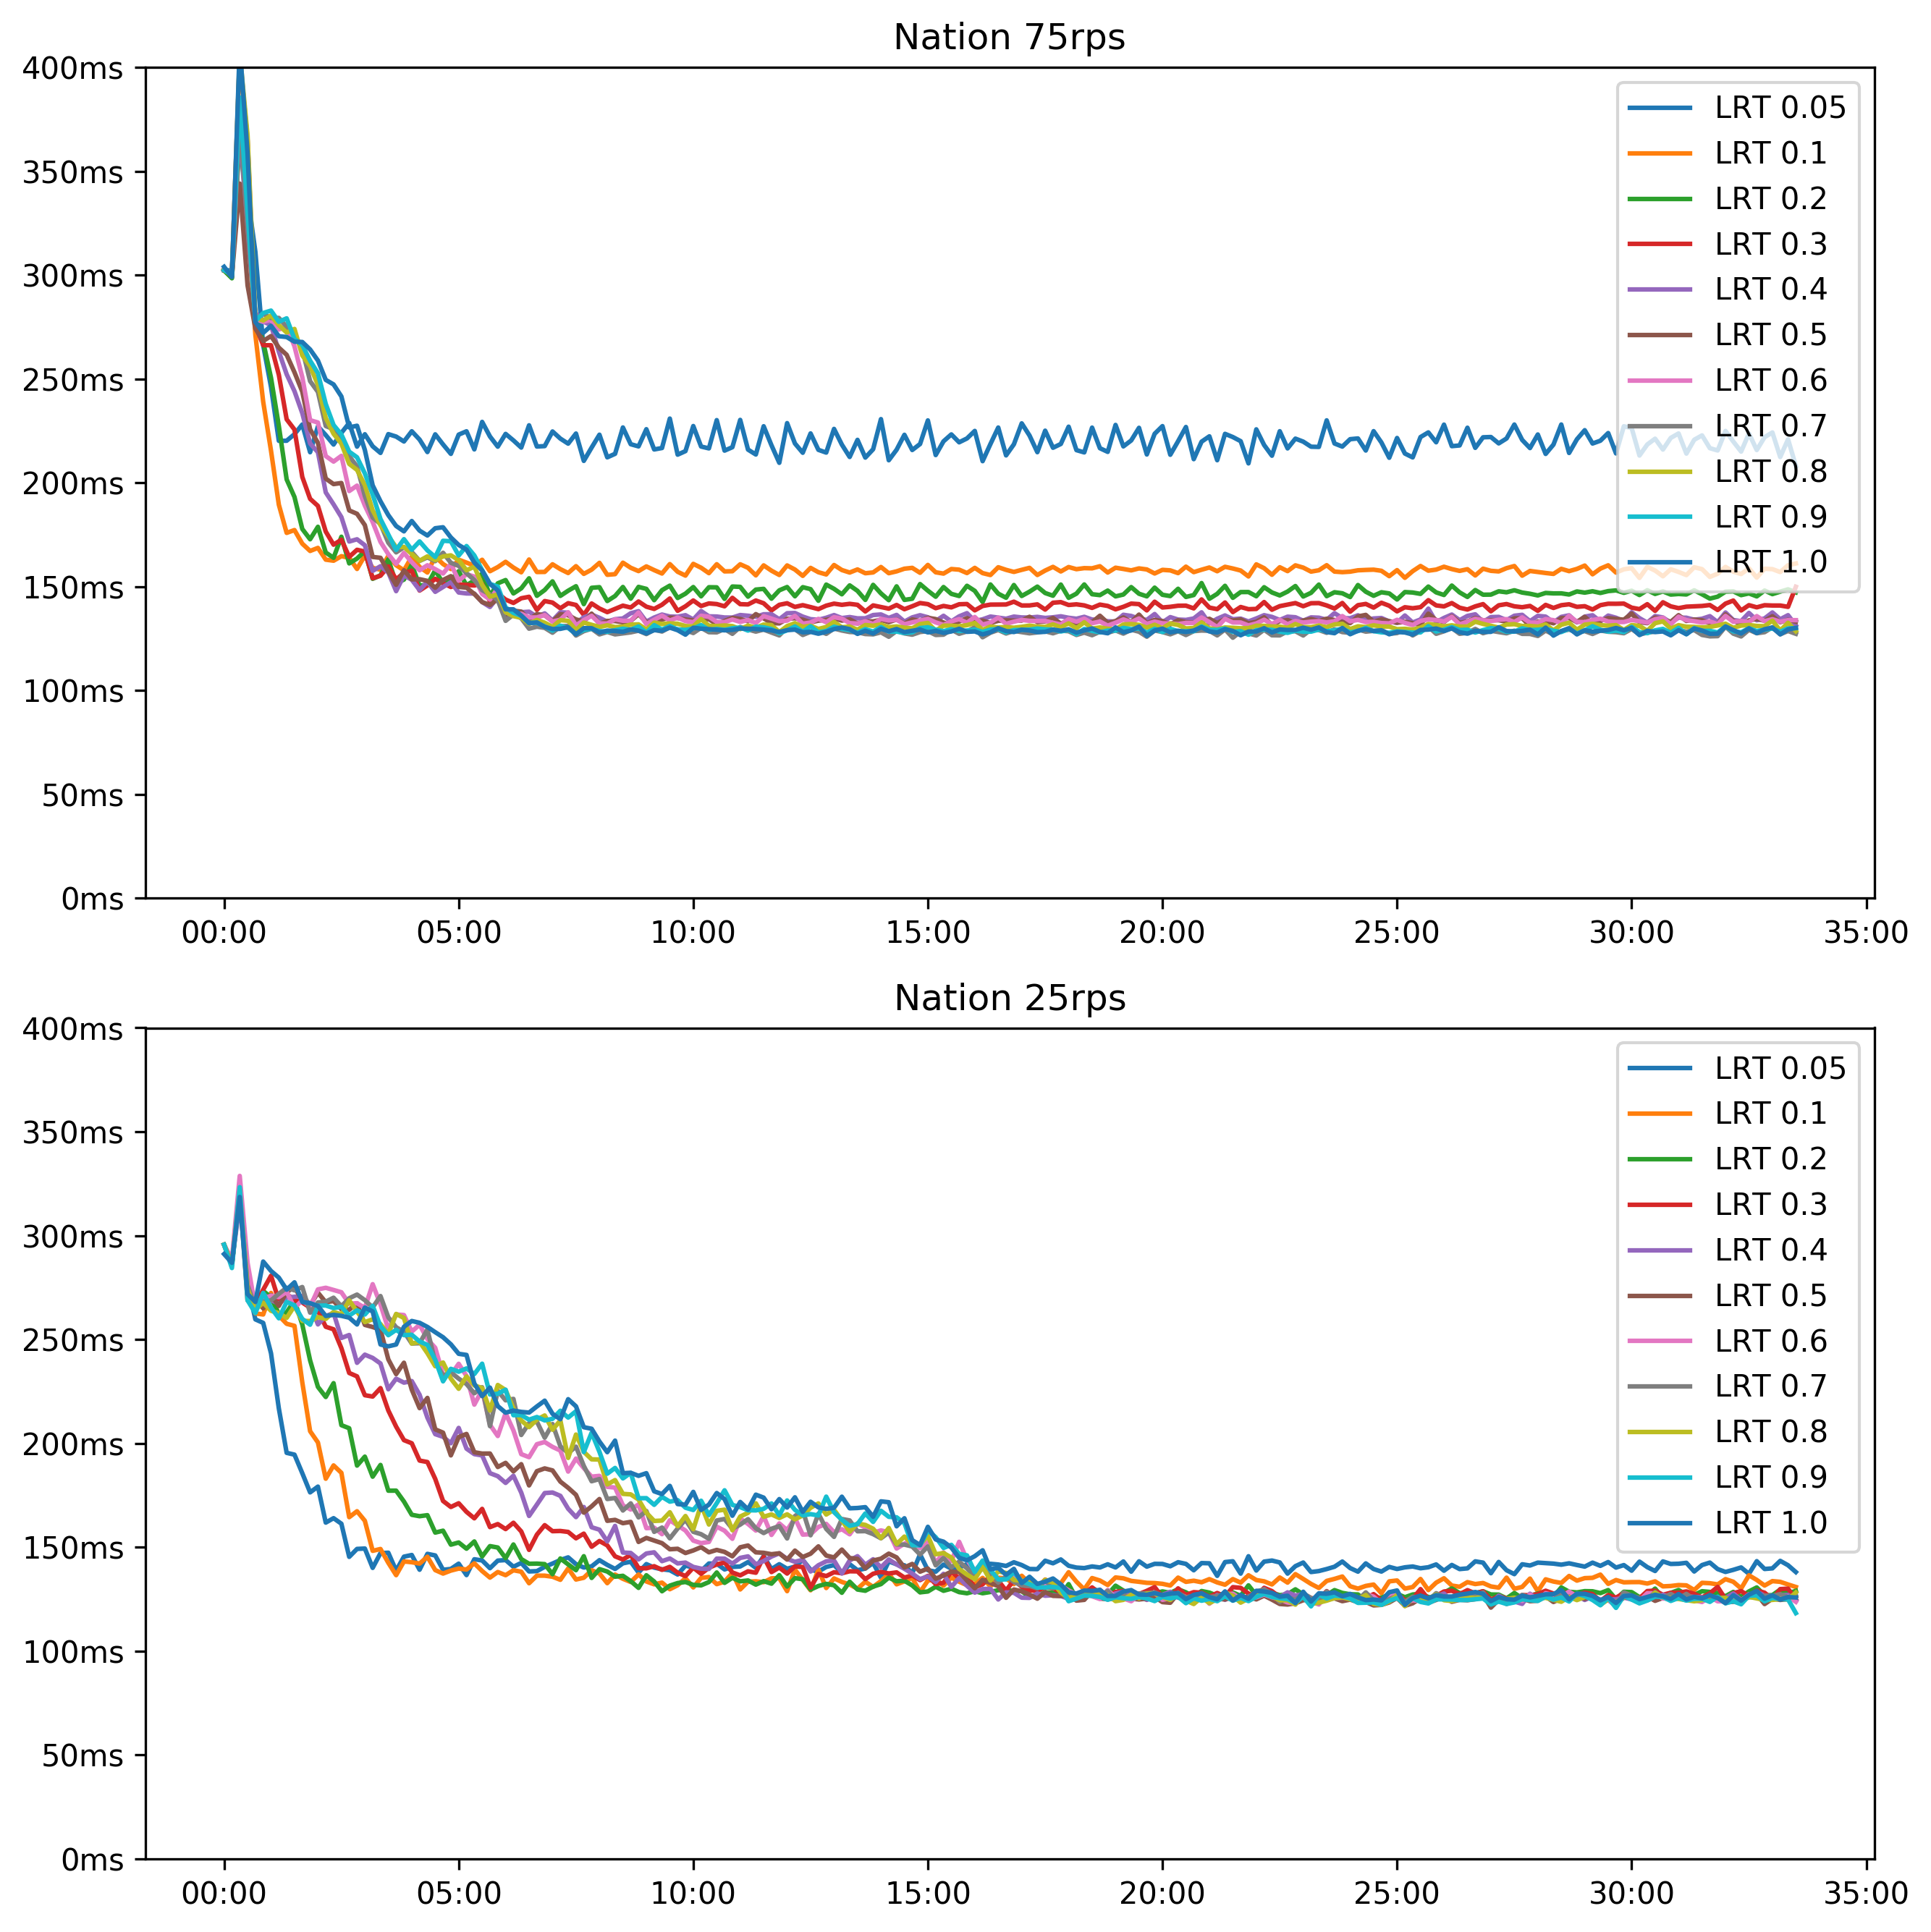
\includegraphics[width=\linewidth]{graphics/graphs/nation_lb_scale.png}
    \caption{\glspl{trt} of different load balancer scales in the nation scenario. For legibility a 10 second moving average is applied.}
    \label{fig:lb_scale_nation}
\end{figure}

Our results show consistent patterns across both topologies, but differ across the request rate.
While in scenarios with a request rate of 75 \gls{rps} higher numbers of load balancers lead to improved mean response time, in scenarios with 25 \gls{rps} lower numbers perform better.
Figures \ref{fig:lb_scale_global} and \ref{fig:lb_scale_nation} show explanations for this behaviour.
With lower numbers of load balancers the request rate per load balancer is higher, and thus leads to faster convergence towards a stable and efficient response time.

Table \ref{tab:lb_scaling_converged_trt} shows the mean response times of different load balancer scales once response times have stabilized.
Once only stabilized values are considered higher numbers of load balancers lead to improved performance.
Figures \ref{fig:lb_scale_global} and \ref{fig:lb_scale_nation} show this too, where lower numbers of load balancers stabilize earlier, but at higher \gls{trt} values.
From Table \ref{tab:lb_scaling_converged_trt} we also see that between the different load balancer scales, differences in response time become negligible at a certain point, with load balancers on 50\% of nodes converging to almost the same mean response time as having load balancers on 100\% of nodes.

Lastly, we observe that the absolute difference between the time when the system performs best, and when the system performs worst is dependent on topology make up.
The globally distributed scenario has the potential to perform worse, as there is a greater likelihood of poor request routing decisions resulting in longer network distances.
\DIFdelbegin %DIFDELCMD < \newpage 
%DIFDELCMD <  \newpage %%%
\DIFdelend \DIFaddbegin 



\DIFaddend \section{\DIFdelbegin \DIFdel{Performance of }\DIFdelend Osmotic Scaling and \DIFdelbegin \DIFdel{Load Balancing}\DIFdelend \DIFaddbegin \DIFadd{Scheduling}\DIFaddend }
%DIF <  2 pages \newpage 
 \DIFdelbegin %DIFDELCMD < \newpage %%%
\section{\DIFdel{Optimization Aggressiveness with Osmotic Scaling}}
%DIFAUXCMD
\addtocounter{section}{-1}%DIFAUXCMD
%DIF <  1.5 pages \newpage 
 %DIFDELCMD < \newpage %%%
\section{\DIFdel{Osmotic Scheduling in Dynamic Systems}}
%DIFAUXCMD
\addtocounter{section}{-1}%DIFAUXCMD
%DIF <  3+ pages (complicated setup, no?) \newpage 
%DIF <  target: 8-9ish pages
\DIFdelend \DIFaddbegin \subsection{\DIFadd{Performance of Osmotic Scaling and Load Balancing}}
%DIF >  2 pages
\DIFadd{With this experiment we want to provide baseline performance data for the osmotic scaling and scheduling method we propose. The goal is to show how our proposed solution operates without fine-tuning of parameters, or any other conditions. The experiment should also show how the osmotic scaling and scheduling of load balancers affects other parts of the serverless system, most notably the scaling decisions of regular functions.
}\subsubsection{\DIFadd{Setup}}
\DIFadd{Our experiment setup for these evaluations is once again based on the serverless edge computing simulator we also used for the initial evaluations. To stay consistent we used the same network topologies from the previous experiment that investigated the impact of load balancer scale on the system, meaning we assume clients to typically be connected via a mobile network, and compute resources to be distributed on the edge. The three topologies we tested are once again one scenario with a single city, one with three cities on the same continent, and one with three cities distributed across the globe. The cities chosen, along with the network latencies between them are the same as in the initial evaluation namely Chicago, New York, and Seattle for the nation-distibuted and New York, London, and Sydney for the globally-distributed experiment. The network latencies between them can be seen in tables \ref{tab:initial_nation_pings} and \ref{tab:initial_global_pings} respectively.
}

\DIFadd{To stay consistent with the other experiments, and partially due to performance limitations, we once again tested each topology scenario with 25\mbox{%DIFAUXCMD
\gls{rps}}\hskip0pt%DIFAUXCMD
, 50\mbox{%DIFAUXCMD
\gls{rps}}\hskip0pt%DIFAUXCMD
, and 75\mbox{%DIFAUXCMD
\gls{rps}}\hskip0pt%DIFAUXCMD
. As for the osmotic scaling and scheduling component, we set the pressure threshold for scaling up to 0.025 and the downscaling threshold to 0.03, which can roughly be read as the system requiring an expected \mbox{%DIFAUXCMD
\gls{trt} }\hskip0pt%DIFAUXCMD
improvement of 2.5\% and 3\% to add or remove a load balancer instance on a given node. Bear in mind that this idea of required estimated performance improvement is a mental model to get a more intuitive understanding for the parameters, and is not equivalent to the actual implementation.
}

\DIFadd{The last way in which the experiment setup differs from the previous experiments is that there is a function scheduling component active. While the other experiments purposefully set a fixed scale for each of the serverless functions in the system to avoid it as a confounding variable, these experiments use a dynamic function scaler to show how this type of load balancer scaling and scheduling affects the overall system.
In concrete terms, we set the simulator up to use a set rate of average requests per function replica.
The reasoning behind this choice is that OpenFaaS uses the same methodology as a default configuration, which we use as a stand-in example of serverless computing frameworks in general.
For the osmotic scaling and scheduling parameters we used 0.03 as a scale-up threshold and 0.05 as a scale-down threshold.
}

\subsubsection{\DIFadd{Results}}

\begin{table}[]
\begin{tabular}{lrrrrrr}
\hline
\textbf{\DIFaddFL{Experiment}}  & \textbf{\begin{tabular}[c]{@{}r@{}}\DIFaddFL{LB}\\ \DIFaddFL{replicas}\end{tabular}} & \textbf{\begin{tabular}[c]{@{}r@{}}\DIFaddFL{Converged}\\ \DIFaddFL{Total }\\ \DIFaddFL{Function}\\ \DIFaddFL{Replicas}\end{tabular}} & \textbf{\begin{tabular}[c]{@{}r@{}}\DIFaddFL{Cross-City}\\ \DIFaddFL{Request}\\ \DIFaddFL{Share}\end{tabular}} & \textbf{\begin{tabular}[c]{@{}r@{}}\DIFaddFL{Mean}\\ \DIFaddFL{TRT}\end{tabular}} & \textbf{\begin{tabular}[c]{@{}r@{}}\DIFaddFL{Median}\\ \DIFaddFL{TRT}\end{tabular}} & \textbf{\begin{tabular}[c]{@{}r@{}}\DIFaddFL{Q90}\\ \DIFaddFL{TRT}\end{tabular}} \\ \hline
\DIFaddFL{25rps City LRT       }& \DIFaddFL{6                                                              }& \DIFaddFL{88                                                                                        }& \DIFaddFL{0.0\%                                                                         }& \DIFaddFL{121ms                                                       }& \DIFaddFL{121ms                                                         }& \DIFaddFL{157ms                                                      }\\
\DIFaddFL{25rps City Osmotic   }& \DIFaddFL{24                                                             }& \DIFaddFL{89                                                                                        }& \DIFaddFL{0.0\%                                                                         }& \DIFaddFL{117ms                                                       }& \DIFaddFL{119ms                                                         }& \DIFaddFL{149ms                                                      }\\
\DIFaddFL{25rps City RR        }& \DIFaddFL{6                                                              }& \DIFaddFL{90                                                                                        }& \DIFaddFL{0.0\%                                                                         }& \DIFaddFL{168ms                                                       }& \DIFaddFL{136ms                                                         }& \DIFaddFL{275ms                                                      }\\ \hline
\DIFaddFL{25rps Nation LRT     }& \DIFaddFL{14                                                             }& \DIFaddFL{89                                                                                        }& \DIFaddFL{17.0\%                                                                        }& \DIFaddFL{154ms                                                       }& \DIFaddFL{131ms                                                         }& \DIFaddFL{254ms                                                      }\\
\DIFaddFL{25rps Nation Osmotic }& \DIFaddFL{3                                                              }& \DIFaddFL{88                                                                                        }& \DIFaddFL{32.5\%                                                                        }& \DIFaddFL{224ms                                                       }& \DIFaddFL{208ms                                                         }& \DIFaddFL{386ms                                                      }\\
\DIFaddFL{25rps Nation RR      }& \DIFaddFL{14                                                             }& \DIFaddFL{90                                                                                        }& \DIFaddFL{65.4\%                                                                        }& \DIFaddFL{274ms                                                       }& \DIFaddFL{266ms                                                         }& \DIFaddFL{432ms                                                      }\\ \hline
\DIFaddFL{25rps Global LRT     }& \DIFaddFL{14                                                             }& \DIFaddFL{94                                                                                        }& \DIFaddFL{0.4\%                                                                         }& \DIFaddFL{142ms                                                       }& \DIFaddFL{126ms                                                         }& \DIFaddFL{210ms                                                      }\\
\DIFaddFL{25rps Global Osmotic }& \DIFaddFL{5                                                              }& \DIFaddFL{90                                                                                        }& \DIFaddFL{1.7\%                                                                         }& \DIFaddFL{152ms                                                       }& \DIFaddFL{128ms                                                         }& \DIFaddFL{224ms                                                      }\\
\DIFaddFL{25rps Global RR      }& \DIFaddFL{14                                                             }& \DIFaddFL{99                                                                                        }& \DIFaddFL{65.4\%                                                                        }& \DIFaddFL{501ms                                                       }& \DIFaddFL{410ms                                                         }& \DIFaddFL{937ms                                                      }\\ \hline
\DIFaddFL{50rps City LRT       }& \DIFaddFL{6                                                              }& \DIFaddFL{249                                                                                       }& \DIFaddFL{0.0\%                                                                         }& \DIFaddFL{127ms                                                       }& \DIFaddFL{124ms                                                         }& \DIFaddFL{177ms                                                      }\\
\DIFaddFL{50rps City Osmotic   }& \DIFaddFL{13                                                             }& \DIFaddFL{249                                                                                       }& \DIFaddFL{0.0\%                                                                         }& \DIFaddFL{123ms                                                       }& \DIFaddFL{123ms                                                         }& \DIFaddFL{164ms                                                      }\\
\DIFaddFL{50rps City RR        }& \DIFaddFL{6                                                              }& \DIFaddFL{249                                                                                       }& \DIFaddFL{0.0\%                                                                         }& \DIFaddFL{162ms                                                       }& \DIFaddFL{141ms                                                         }& \DIFaddFL{248ms                                                      }\\ \hline
\DIFaddFL{50rps Nation LRT     }& \DIFaddFL{14                                                             }& \DIFaddFL{179                                                                                       }& \DIFaddFL{17.7\%                                                                        }& \DIFaddFL{153ms                                                       }& \DIFaddFL{129ms                                                         }& \DIFaddFL{270ms                                                      }\\
\DIFaddFL{50rps Nation Osmotic }& \DIFaddFL{5                                                              }& \DIFaddFL{177                                                                                       }& \DIFaddFL{24.3\%                                                                        }& \DIFaddFL{165ms                                                       }& \DIFaddFL{135ms                                                         }& \DIFaddFL{283ms                                                      }\\
\DIFaddFL{50rps Nation RR      }& \DIFaddFL{14                                                             }& \DIFaddFL{181                                                                                       }& \DIFaddFL{65.0\%                                                                        }& \DIFaddFL{271ms                                                       }& \DIFaddFL{264ms                                                         }& \DIFaddFL{430ms                                                      }\\ \hline
\DIFaddFL{50rps Global LRT     }& \DIFaddFL{14                                                             }& \DIFaddFL{190                                                                                       }& \DIFaddFL{1.2\%                                                                         }& \DIFaddFL{147ms                                                       }& \DIFaddFL{128ms                                                         }& \DIFaddFL{213ms                                                      }\\
\DIFaddFL{50rps Global Osmotic }& \DIFaddFL{4                                                              }& \DIFaddFL{181                                                                                       }& \DIFaddFL{3.8\%                                                                         }& \DIFaddFL{159ms                                                       }& \DIFaddFL{128ms                                                         }& \DIFaddFL{238ms                                                      }\\
\DIFaddFL{50rps Global RR      }& \DIFaddFL{14                                                             }& \DIFaddFL{197                                                                                       }& \DIFaddFL{65.1\%                                                                        }& \DIFaddFL{494ms                                                       }& \DIFaddFL{410ms                                                         }& \DIFaddFL{922ms                                                      }\\ \hline
\DIFaddFL{75rps City LRT       }& \DIFaddFL{6                                                              }& \DIFaddFL{249                                                                                       }& \DIFaddFL{0.0\%                                                                         }& \DIFaddFL{127ms                                                       }& \DIFaddFL{123ms                                                         }& \DIFaddFL{175ms                                                      }\\
\DIFaddFL{75rps City Osmotic   }& \DIFaddFL{14                                                             }& \DIFaddFL{249                                                                                       }& \DIFaddFL{0.0\%                                                                         }& \DIFaddFL{122ms                                                       }& \DIFaddFL{122ms                                                         }& \DIFaddFL{162ms                                                      }\\
\DIFaddFL{75rps City RR        }& \DIFaddFL{6                                                              }& \DIFaddFL{249                                                                                       }& \DIFaddFL{0.0\%                                                                         }& \DIFaddFL{168ms                                                       }& \DIFaddFL{140ms                                                         }& \DIFaddFL{275ms                                                      }\\ \hline
\DIFaddFL{75rps Nation LRT     }& \DIFaddFL{14                                                             }& \DIFaddFL{269                                                                                       }& \DIFaddFL{14.9\%                                                                        }& \DIFaddFL{150ms                                                       }& \DIFaddFL{129ms                                                         }& \DIFaddFL{260ms                                                      }\\
\DIFaddFL{75rps Nation Osmotic }& \DIFaddFL{5                                                              }& \DIFaddFL{264                                                                                       }& \DIFaddFL{24.1\%                                                                        }& \DIFaddFL{169ms                                                       }& \DIFaddFL{138ms                                                         }& \DIFaddFL{287ms                                                      }\\
\DIFaddFL{75rps Nation RR      }& \DIFaddFL{14                                                             }& \DIFaddFL{269                                                                                       }& \DIFaddFL{65.2\%                                                                        }& \DIFaddFL{273ms                                                       }& \DIFaddFL{269ms                                                         }& \DIFaddFL{433ms                                                      }\\ \hline
\DIFaddFL{75rps Global LRT     }& \DIFaddFL{14                                                             }& \DIFaddFL{278                                                                                       }& \DIFaddFL{0.1\%                                                                         }& \DIFaddFL{141ms                                                       }& \DIFaddFL{128ms                                                         }& \DIFaddFL{214ms                                                      }\\
\DIFaddFL{75rps Global Osmotic }& \DIFaddFL{5                                                              }& \DIFaddFL{268                                                                                       }& \DIFaddFL{1.9\%                                                                         }& \DIFaddFL{152ms                                                       }& \DIFaddFL{129ms                                                         }& \DIFaddFL{223ms                                                      }\\
\DIFaddFL{75rps Global RR      }& \DIFaddFL{14                                                             }& \DIFaddFL{285                                                                                       }& \DIFaddFL{65.2\%                                                                        }& \DIFaddFL{497ms                                                       }& \DIFaddFL{406ms                                                         }& \DIFaddFL{928ms                                                      }\\ \hline
\end{tabular}
\caption{\DIFaddFL{Osmotic baseline evaluation results}}
\label{tab:osmotic_base}
\end{table}

\begin{figure}
    \centering
    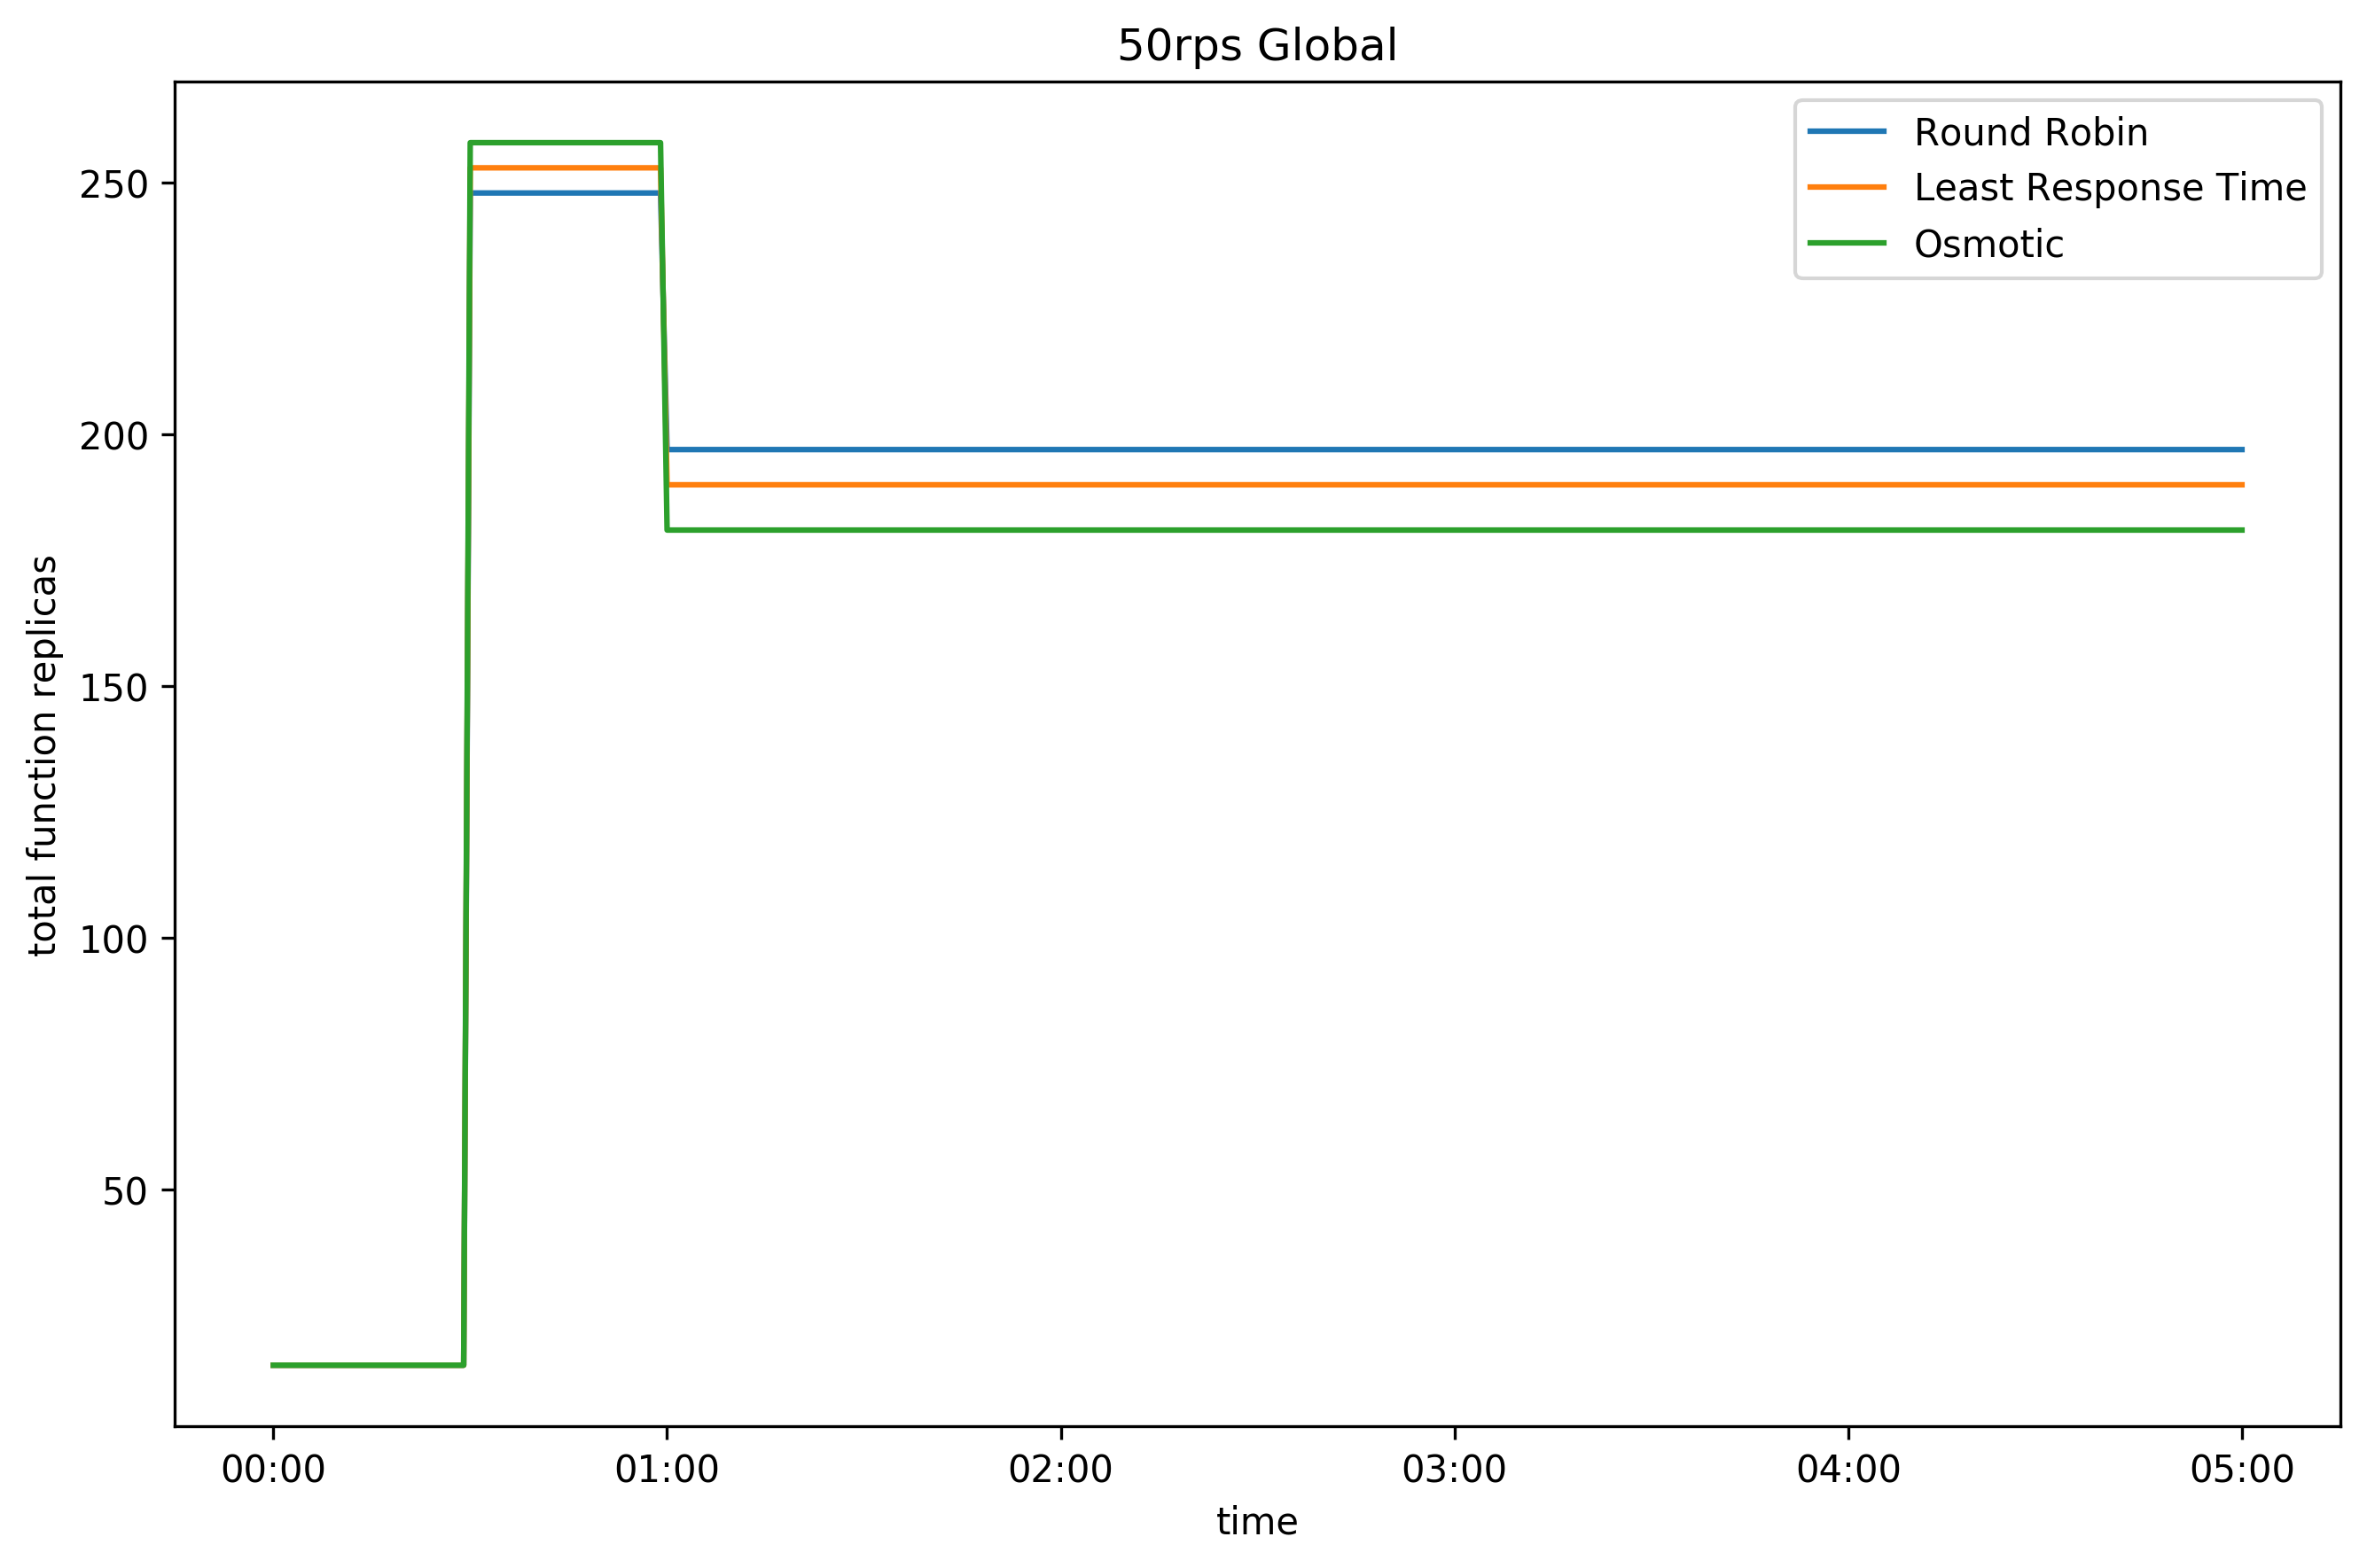
\includegraphics[width=12cm]{graphics/graphs/osmotic_base_function_scale_by_lb.png}
    \caption{\DIFaddFL{Total scale of all functions for each load balancer scaling/schedulilng method}}
    \label{fig:osmotic_fx_scale_by_scaling}
\end{figure}

\DIFadd{Table \ref{tab:osmotic_base} shows the results of the experiment.
In terms of mean \mbox{%DIFAUXCMD
\gls{trt} }\hskip0pt%DIFAUXCMD
performance the results of our proposed osmotic scaling and scheduling method are similar to those of the fixed scaling LRT reference setup, albeit between 1\% and 45\% worse with most scenarios only between 2\% and 8\% worse.
Differences between least response time static, and osmotic scaling are less pronounced in the median and 90th percentile \mbox{%DIFAUXCMD
\glspl{trt} }\hskip0pt%DIFAUXCMD
as can also be seen in Table \ref{tab:osmotic_base}.
The statically scaled round robin load balancing is, as one would expect, significantly worse.
It does, however, give a good impression of the performance improvements possible based on our approach in a more complex and realistic deployment scenario than the initial evaluation.
}

\DIFadd{We can also observe that in the city scenario the osmotic scaling and scheduling ends up deploying the more load balancer instances than the static scaling, but that for the nation- and globally-distributed network topology scenarios this patterns is reversed. There the osmotic scaler deploys only about a third of the replicas of the static scaling.
}

\DIFadd{A similar pattern can be seen with regard to function scaling.
The osmotic scaling leads to between 1\% and 6\% fewer function replicas being deployed. Figure \ref{fig:osmotic_fx_scale_by_scaling} shows how the timing and frequency of scaling decisions are not different between the scaling methods, but osmotic scaling results in slightly fewer function replicas. 
}\subsection{\DIFadd{Optimization Aggressiveness with Osmotic Scaling}}
\DIFadd{We already learned from the experiment about load balancer scale that there is a tendency for a higher scale of load balancers to ultimately result in better performance.
With this experiment we want to test the interplay of this phenomenon with the osmotic load balancing and scaling we propose. With our osmotic approach we can set the scale-up threshold to more or less arbitrary values to influence how quickly or slowly the system scales up the number of load balancers, and how many load balancers will thus ultimately end up being deployed.
}

\subsubsection{\DIFadd{Setup}}
\DIFadd{To test the performance we simulate a number of different configuration scenarios. For the rest of the system environment we choose to reuse the globally distributed topology from previous experiments with a request rate of 75\mbox{%DIFAUXCMD
\gls{rps} }\hskip0pt%DIFAUXCMD
being simulated over the course of 2000 seconds.
}

\DIFadd{For the parameters of the osmotic scaling and scheduling we run experiments for a range of scale-up thresholds ranging from 0.02 to 0.1.
The scale down threshold is always set to 0.2, which is relatively high, because we explicitly want to test how the scale-up threshold can be used to determine how many load balancers the system will deploy to optimize response times.
}

\subsubsection{\DIFadd{Results}}

\begin{table}[]
\begin{tabular}{lrrrrr}
\hline
\textbf{\begin{tabular}[c]{@{}l@{}}\DIFaddFL{Upscaling}\\ \DIFaddFL{Pressure}\\ \DIFaddFL{Threshold}\end{tabular}} & \textbf{\begin{tabular}[c]{@{}r@{}}\DIFaddFL{LB}\\ \DIFaddFL{Replicas}\end{tabular}} & \textbf{\begin{tabular}[c]{@{}r@{}}\DIFaddFL{Mean}\\ \DIFaddFL{TRT}\end{tabular}} & \textbf{\begin{tabular}[c]{@{}r@{}}\DIFaddFL{Mean}\\ \DIFaddFL{FET}\end{tabular}} & \textbf{\begin{tabular}[c]{@{}r@{}}\DIFaddFL{Mean}\\ \DIFaddFL{LB\_FX}\end{tabular}} & \textbf{\begin{tabular}[c]{@{}r@{}}\DIFaddFL{Mean}\\ \DIFaddFL{CL\_LB}\end{tabular}} \\ \hline
\DIFaddFL{0.1                                                                               }& \DIFaddFL{4                                                              }& \DIFaddFL{155.8ms                                                     }& \DIFaddFL{29.1ms                                                      }& \DIFaddFL{33.5ms                                                         }& \DIFaddFL{92.7ms                                                         }\\
\DIFaddFL{0.09                                                                              }& \DIFaddFL{4                                                              }& \DIFaddFL{152.5ms                                                     }& \DIFaddFL{29.7ms                                                      }& \DIFaddFL{30.1ms                                                         }& \DIFaddFL{92.2ms                                                         }\\
\DIFaddFL{0.08                                                                              }& \DIFaddFL{6                                                              }& \DIFaddFL{152.1ms                                                     }& \DIFaddFL{29.5ms                                                      }& \DIFaddFL{30.0ms                                                         }& \DIFaddFL{92.2ms                                                         }\\
\DIFaddFL{0.07                                                                              }& \DIFaddFL{5                                                              }& \DIFaddFL{152.5ms                                                     }& \DIFaddFL{29.3ms                                                      }& \DIFaddFL{30.4ms                                                         }& \DIFaddFL{92.4ms                                                         }\\
\DIFaddFL{0.06                                                                              }& \DIFaddFL{5                                                              }& \DIFaddFL{148.5ms                                                     }& \DIFaddFL{29.6ms                                                      }& \DIFaddFL{26.6ms                                                         }& \DIFaddFL{91.6ms                                                         }\\
\DIFaddFL{0.05                                                                              }& \DIFaddFL{5                                                              }& \DIFaddFL{147.5ms                                                     }& \DIFaddFL{29.9ms                                                      }& \DIFaddFL{25.3ms                                                         }& \DIFaddFL{91.3ms                                                         }\\
\DIFaddFL{0.04                                                                              }& \DIFaddFL{5                                                              }& \DIFaddFL{148.5ms                                                     }& \DIFaddFL{29.8ms                                                      }& \DIFaddFL{26.5ms                                                         }& \DIFaddFL{91.5ms                                                         }\\
\DIFaddFL{0.03                                                                              }& \DIFaddFL{7                                                              }& \DIFaddFL{136.8ms                                                     }& \DIFaddFL{26.4ms                                                      }& \DIFaddFL{19.6ms                                                         }& \DIFaddFL{91.2ms                                                         }\\
\DIFaddFL{0.02                                                                              }& \DIFaddFL{20                                                             }& \DIFaddFL{139.0ms                                                     }& \DIFaddFL{24.8ms                                                      }& \DIFaddFL{25.3ms                                                         }& \DIFaddFL{90.2ms                                                         }\\ \hline
\end{tabular}
\caption{\DIFaddFL{Response time performance metrics for different upscaling pressure thresholds}}
\label{tab:osmotic_scaling_aggressiveness}
\end{table}





\begin{figure}
    \centering
    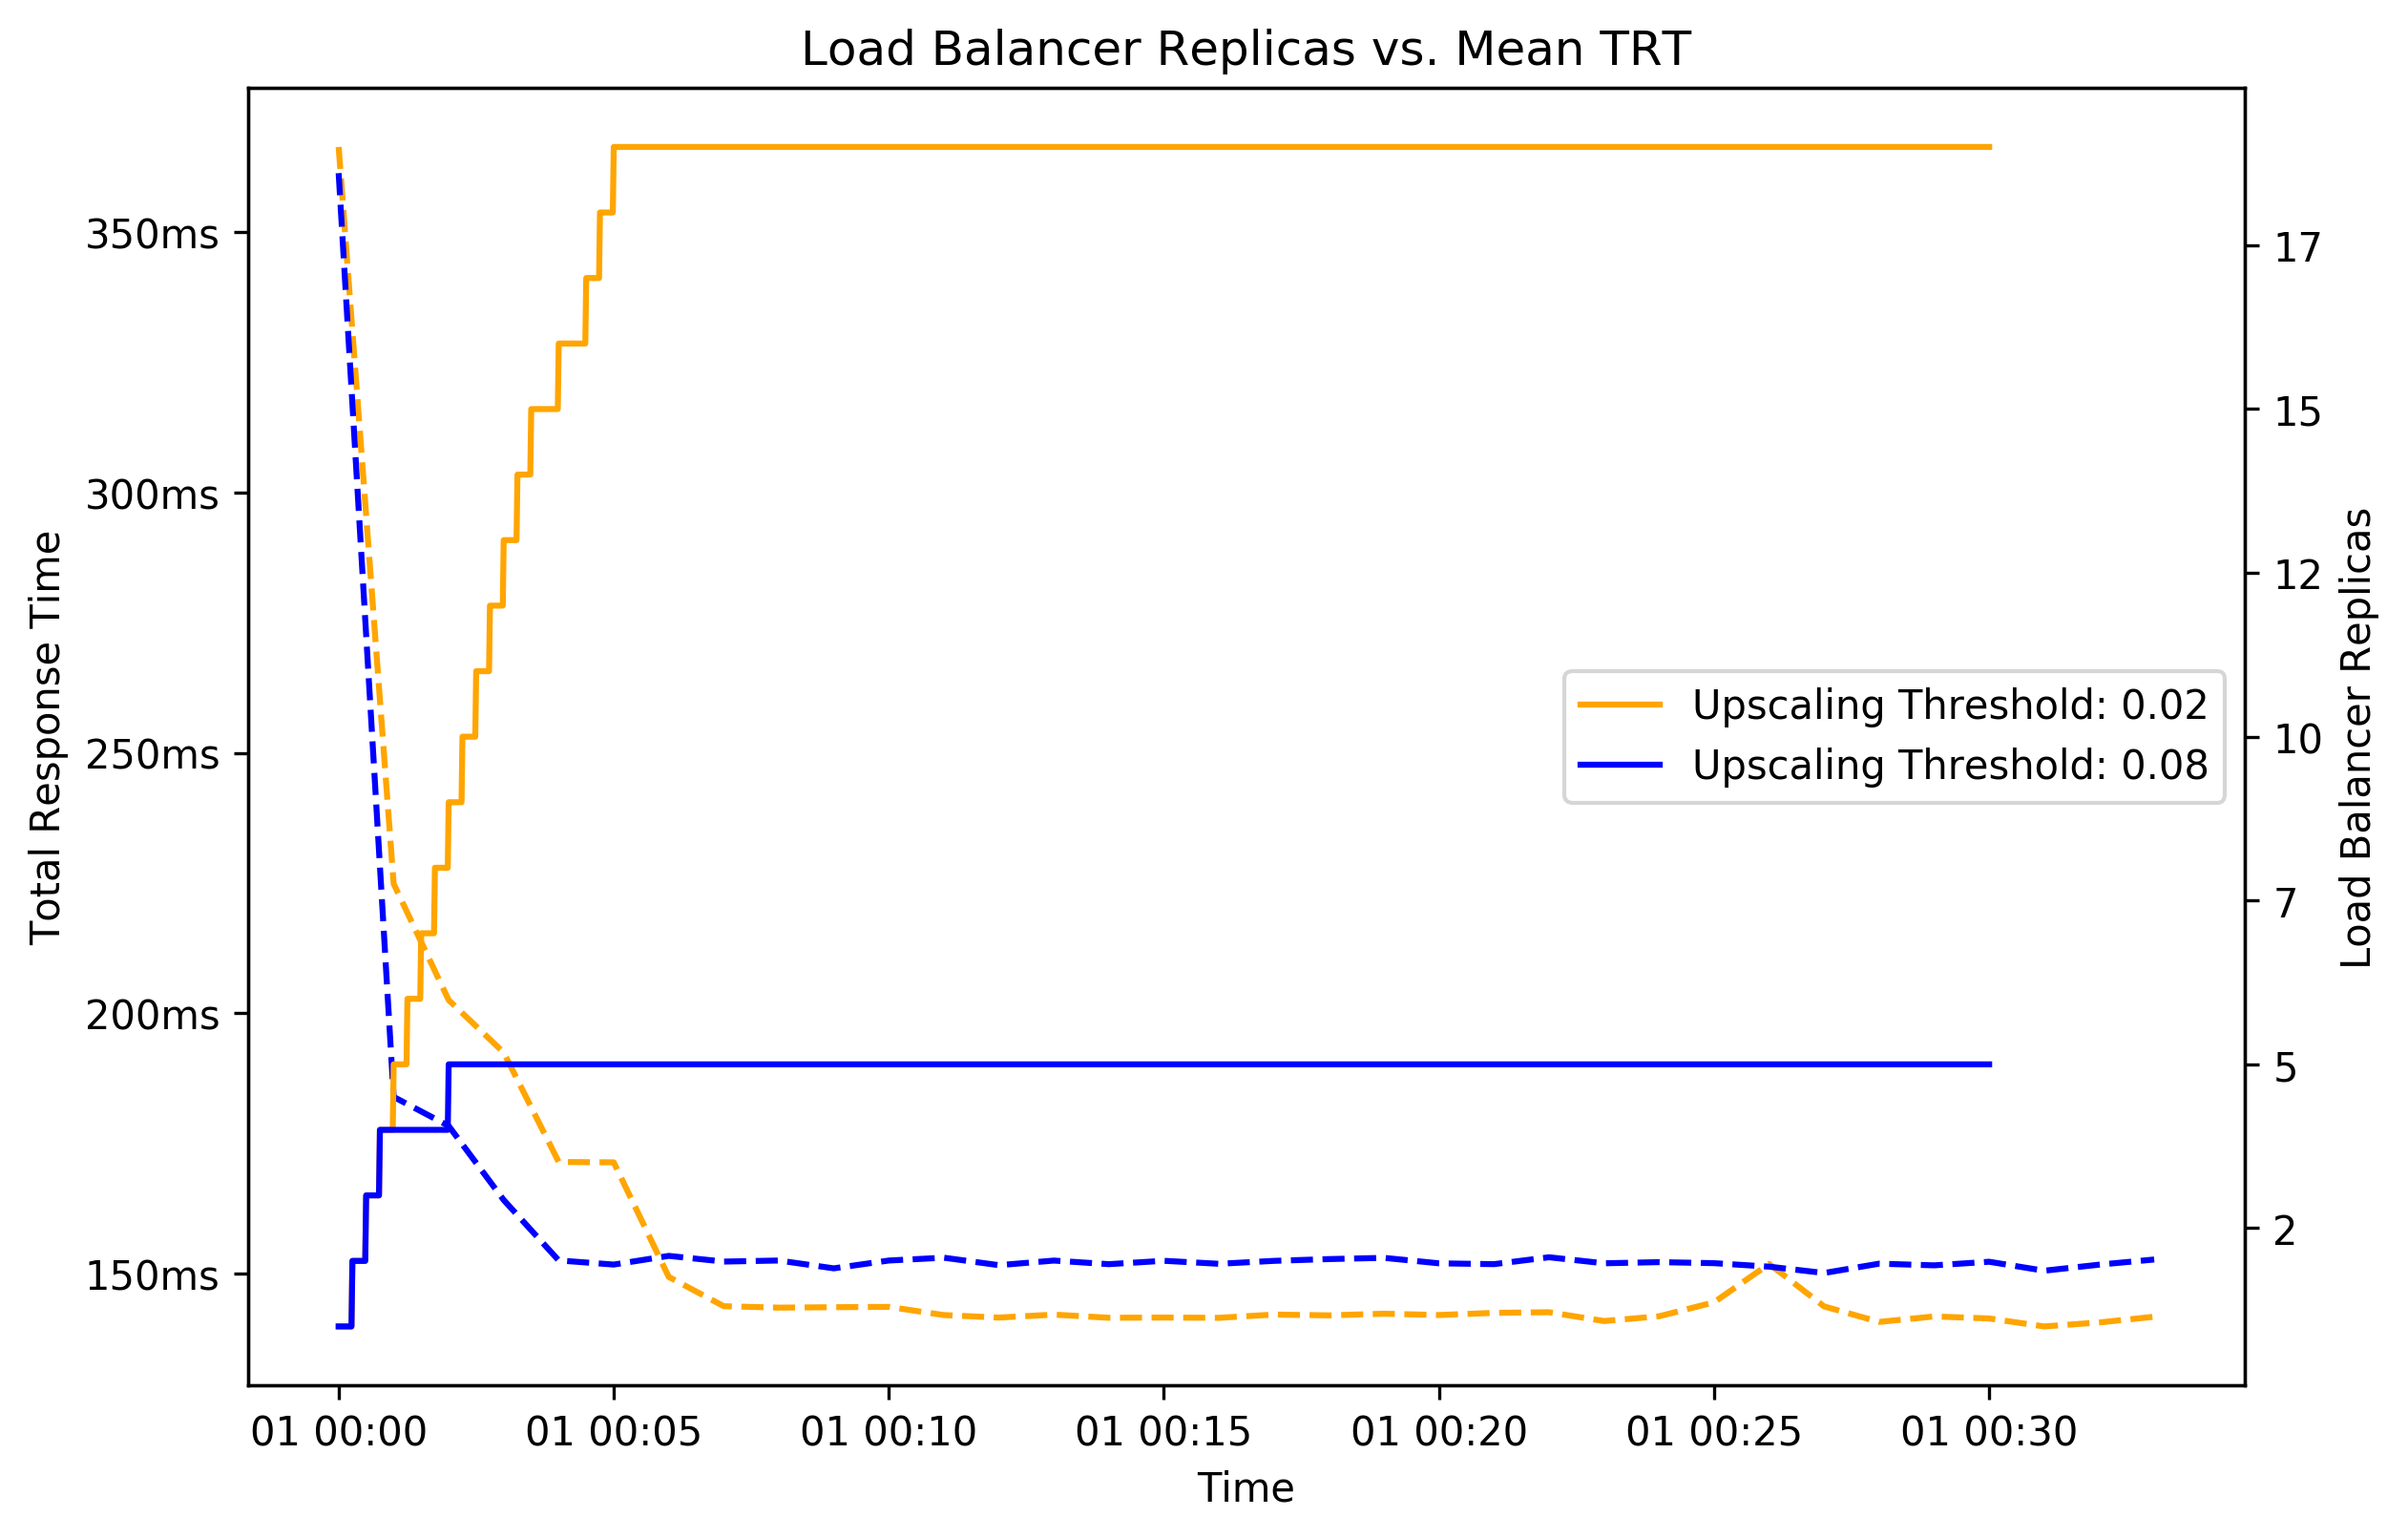
\includegraphics[width=12cm]{graphics/graphs/osmotic_optim_thres_vs_trt.png}
    \caption{\DIFaddFL{\mbox{%DIFAUXCMD
\gls{trt} }\hskip0pt%DIFAUXCMD
compared to current load balancer scale for two different osmotic scaling parametrizations}}
    \label{fig:osmotic_trt_vs_replica_scale}
\end{figure}

\DIFadd{The results show two clear trends.
First that will lower upscaling pressure thresholds more load balancer replicas are being deployed by the osmotic scaling component, and second that the mean response time improves with higher number of load balancer replicas.
As Table \ref{tab:osmotic_scaling_aggressiveness} shows, there is a diminishing return with higher numbers of load balancers, at least in the topology scenario tested.
The results also show that while higher numbers of load balancers provide better performance once the load balancers have gathered enough information about available replicas, this process is faster the fewer load balancers there are, thus giving better performance early on.
The behaviour can be observed easily in the graph in Figure \ref{fig:osmotic_trt_vs_replica_scale}.
}\subsection{\DIFadd{Osmotic Scheduling in Dynamic Systems}}
%DIF >  3+ pages (complicated setup, no?)
\DIFadd{In this last experiment we test the behaviour of our osmotic scaling and scheduling method in a dynamic system.
Since dynamic changes of the system make-up are a core part of edge computing, and our approach is explicitly constructed with these dynamic factors in mind, we believe it is important to test the efficacy of our approach in such a scenario.
Because a lot of components have already been analyzed in-depth, and results are most clear when only one factor is tested at any given time, we choose to use the request origin as the dynamic  system component.
With the experiment we test how our proposed approach handles requests originating from different regions of the overall system over time.
}\subsubsection{\DIFadd{Setup}}
\DIFadd{For this experiment we once again use the globally distributed scenario as our network topology, and apply a constant request rate of 25\mbox{%DIFAUXCMD
\gls{rps}}\hskip0pt%DIFAUXCMD
.
Each of the three cities present in the topology additionally has a probability function associated with it, which determines the chance of a request originating from that city.
These probability functions for the cities are set up in such a way that most of the requests originate from only one of the cities for a given time period.
After some time the active city changes and the requests gradually start to come from another city.
The periods and changes are set up in such a way that over the course of the 2000 second long simulation each of the cities is the main originator of requests at one point.
}

\subsubsection{\DIFadd{Results}}

\begin{figure}
    \centering
    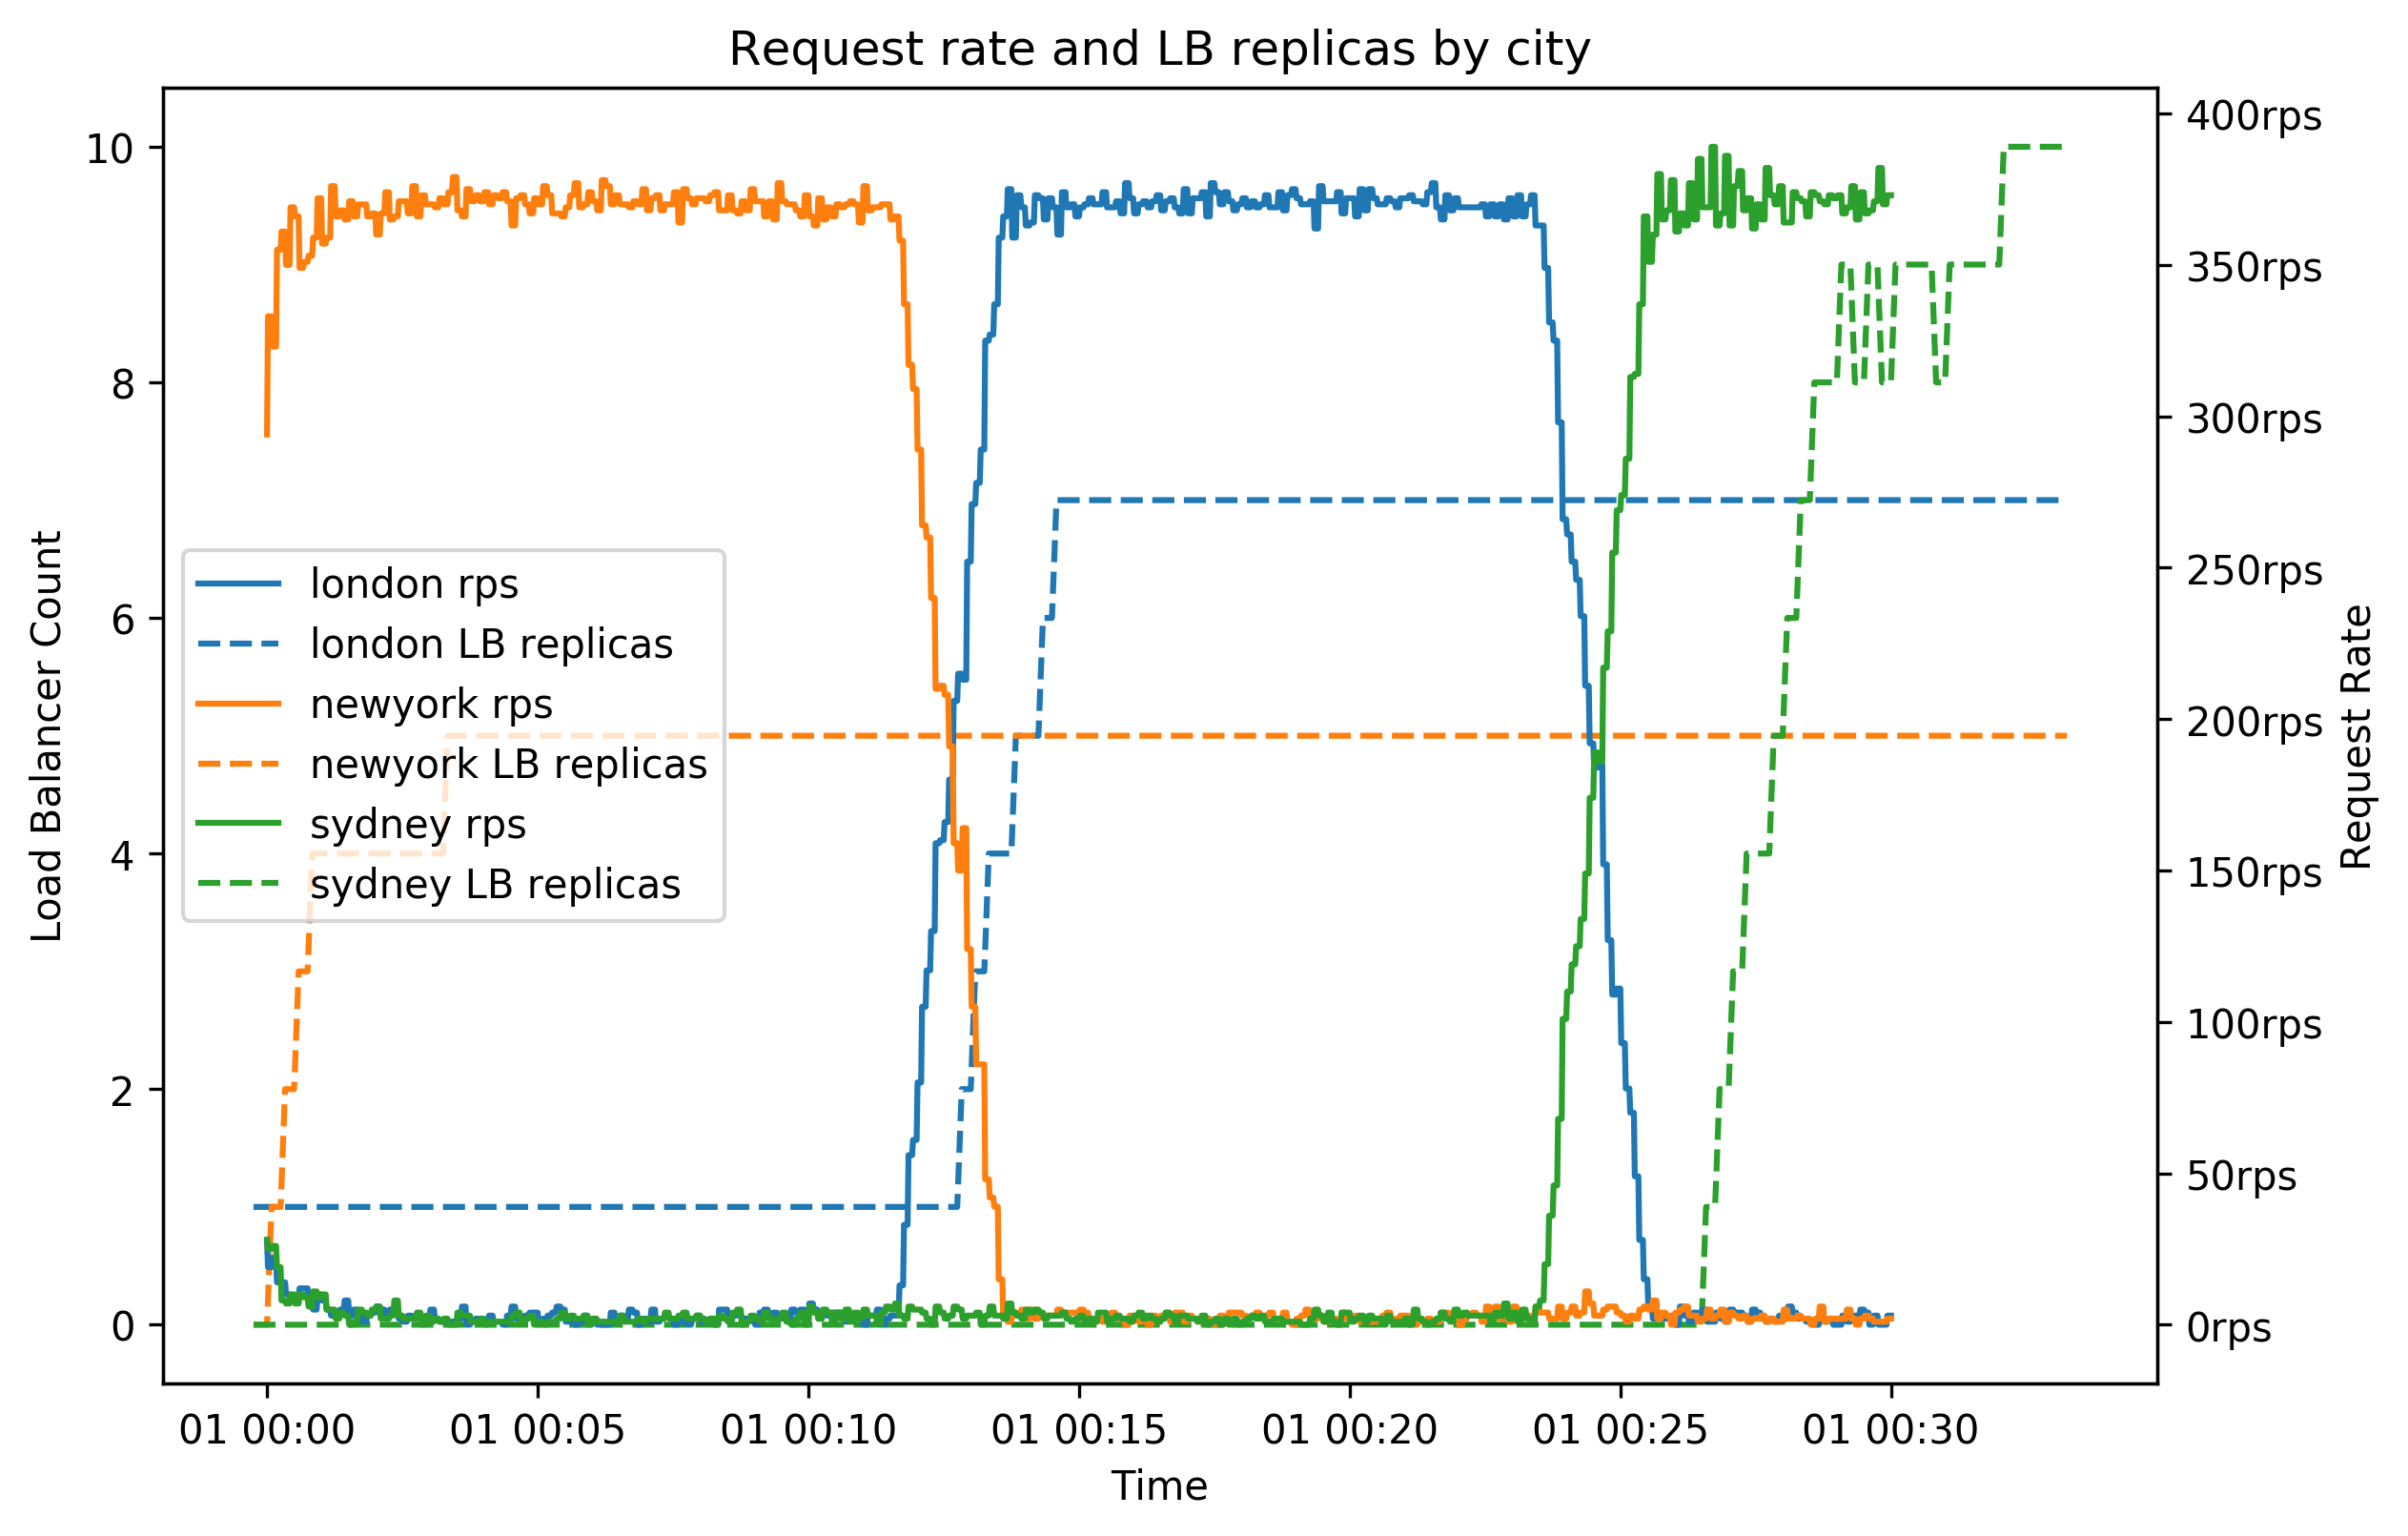
\includegraphics[width=14cm]{graphics/graphs/osmotic_dynamic_region_rps_lb_relicas.png}
    \caption{\DIFaddFL{Load balancer replica count per city over changing request origins}}
    \label{fig:osmotic_dynamic_lb_replicas}
\end{figure}

\begin{figure}
    \centering
    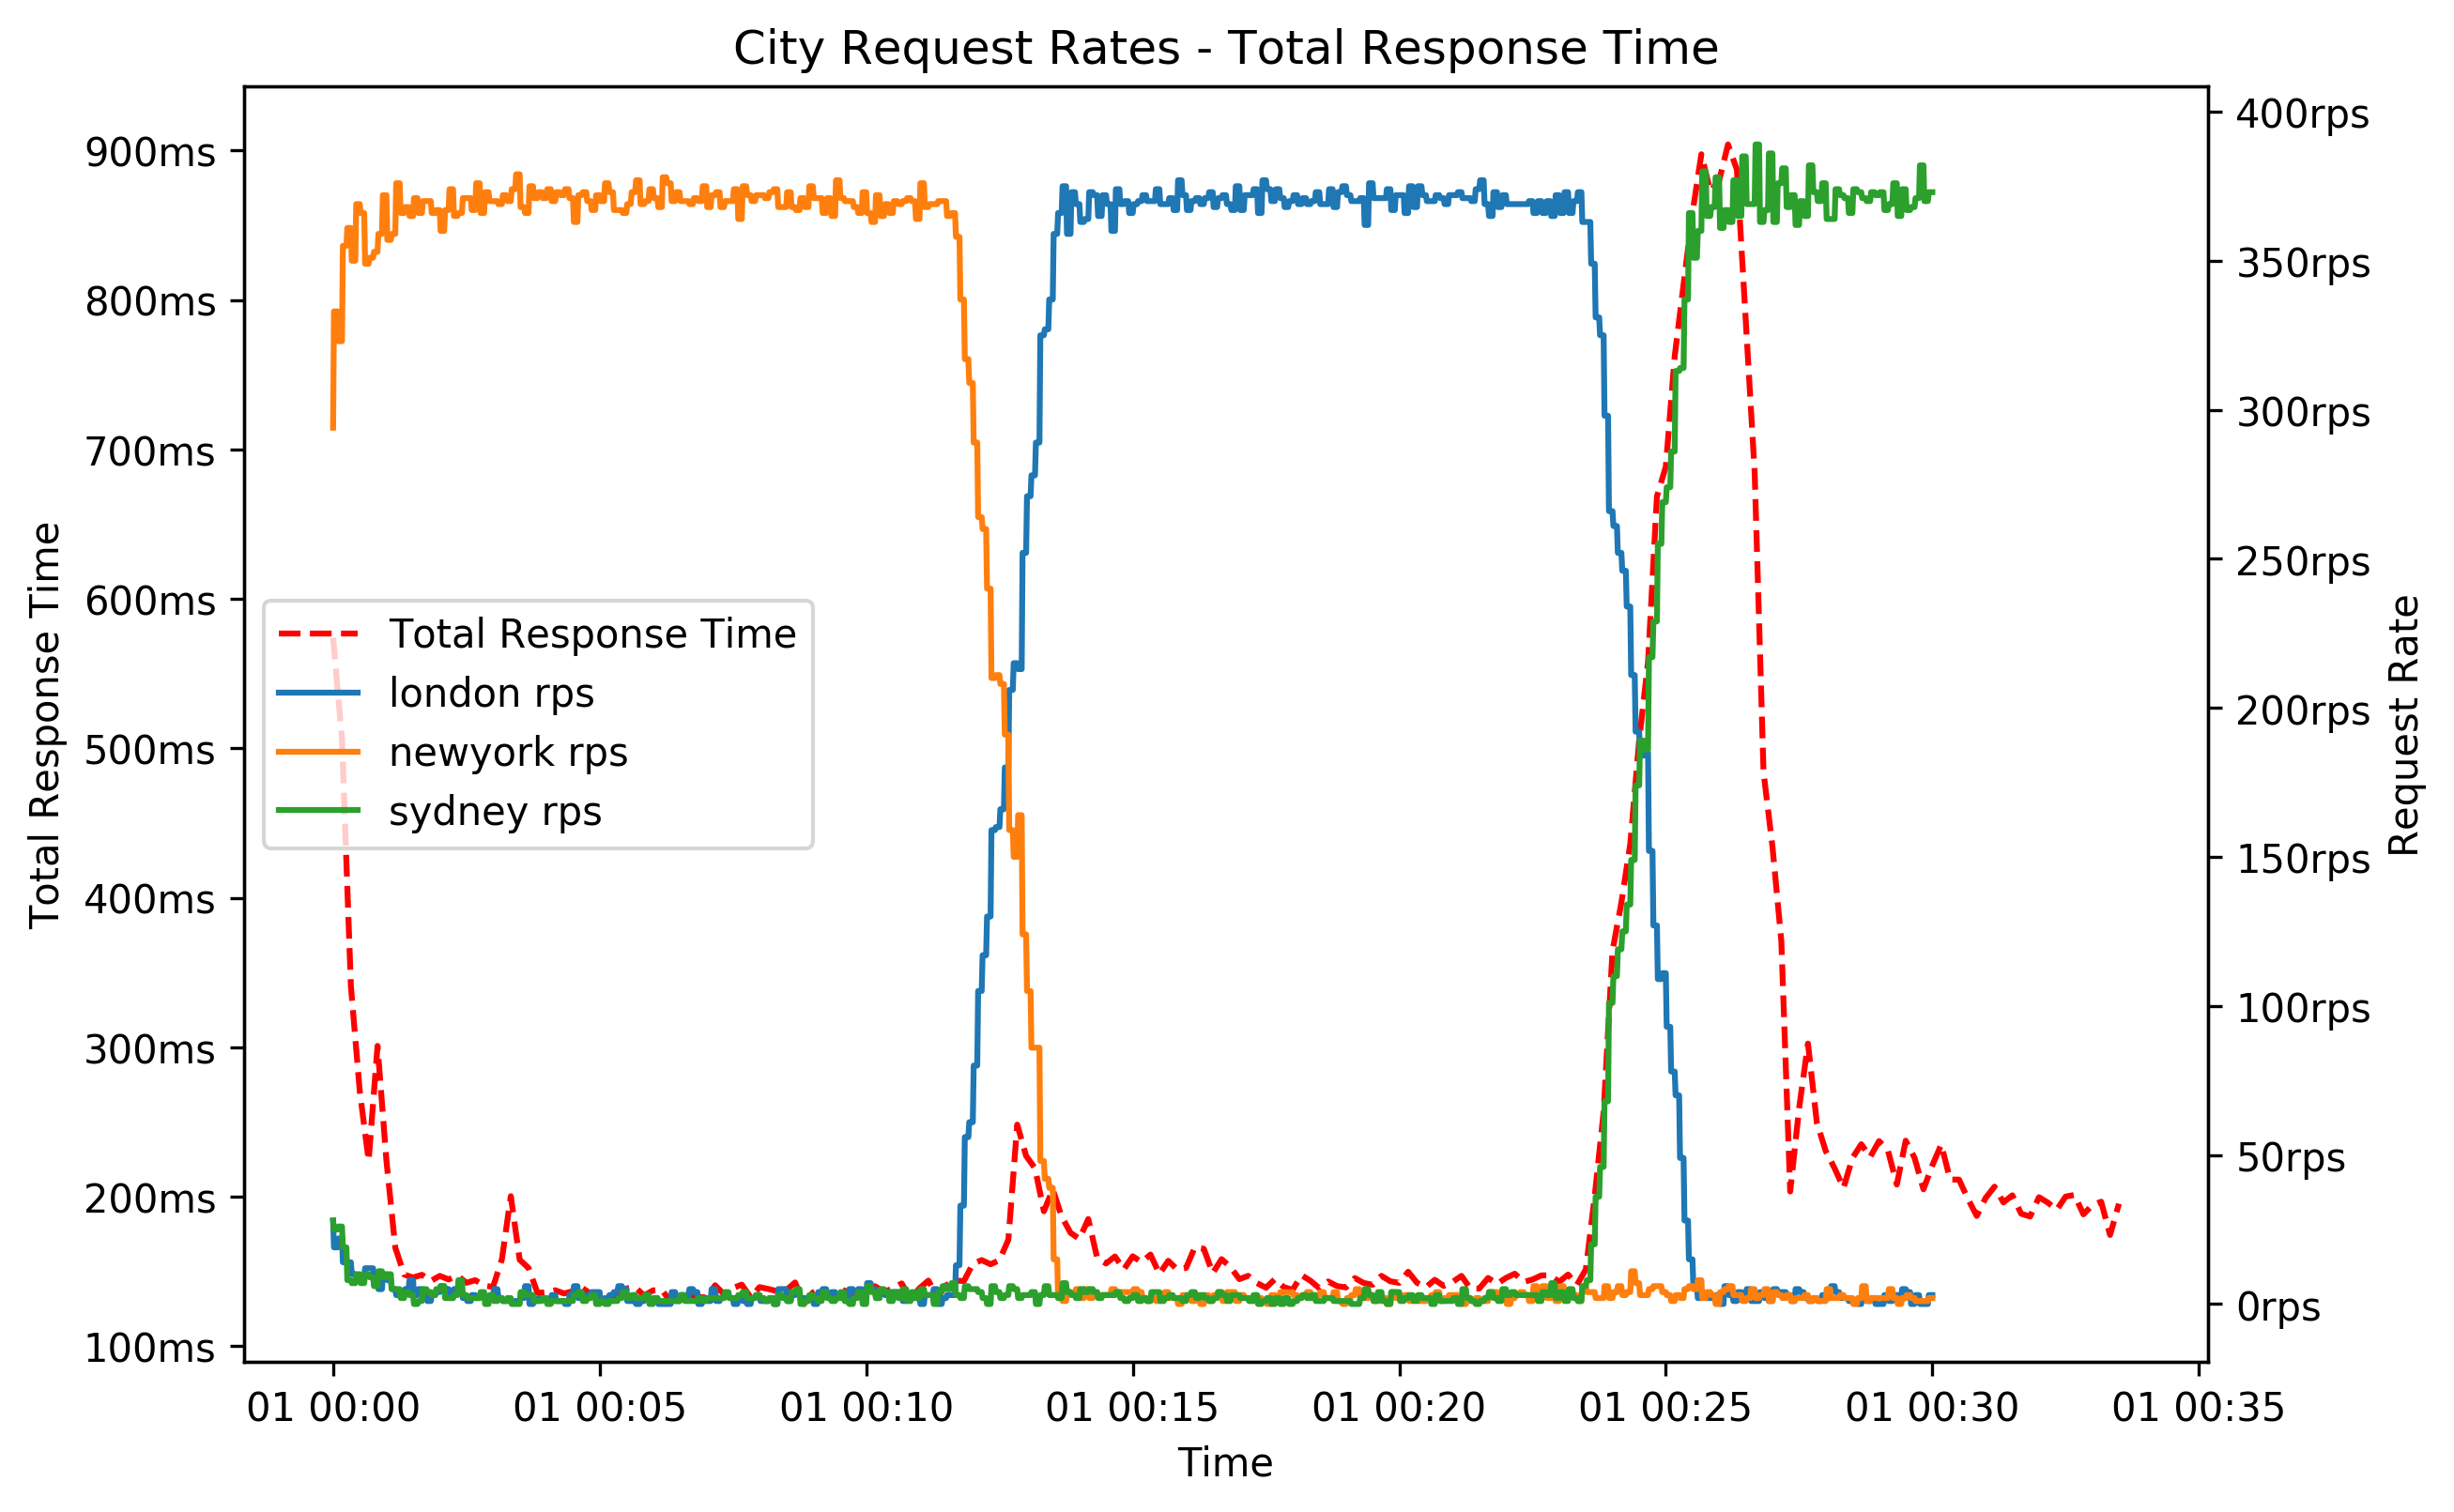
\includegraphics[width=14cm]{graphics/graphs/osmotic_dynamc_region_rps_trt.png}
    \caption{\DIFaddFL{Total response time over changing request origins}}
    \label{fig:osmotic_dynamic_trt}
\end{figure}

\begin{figure}
    \centering
    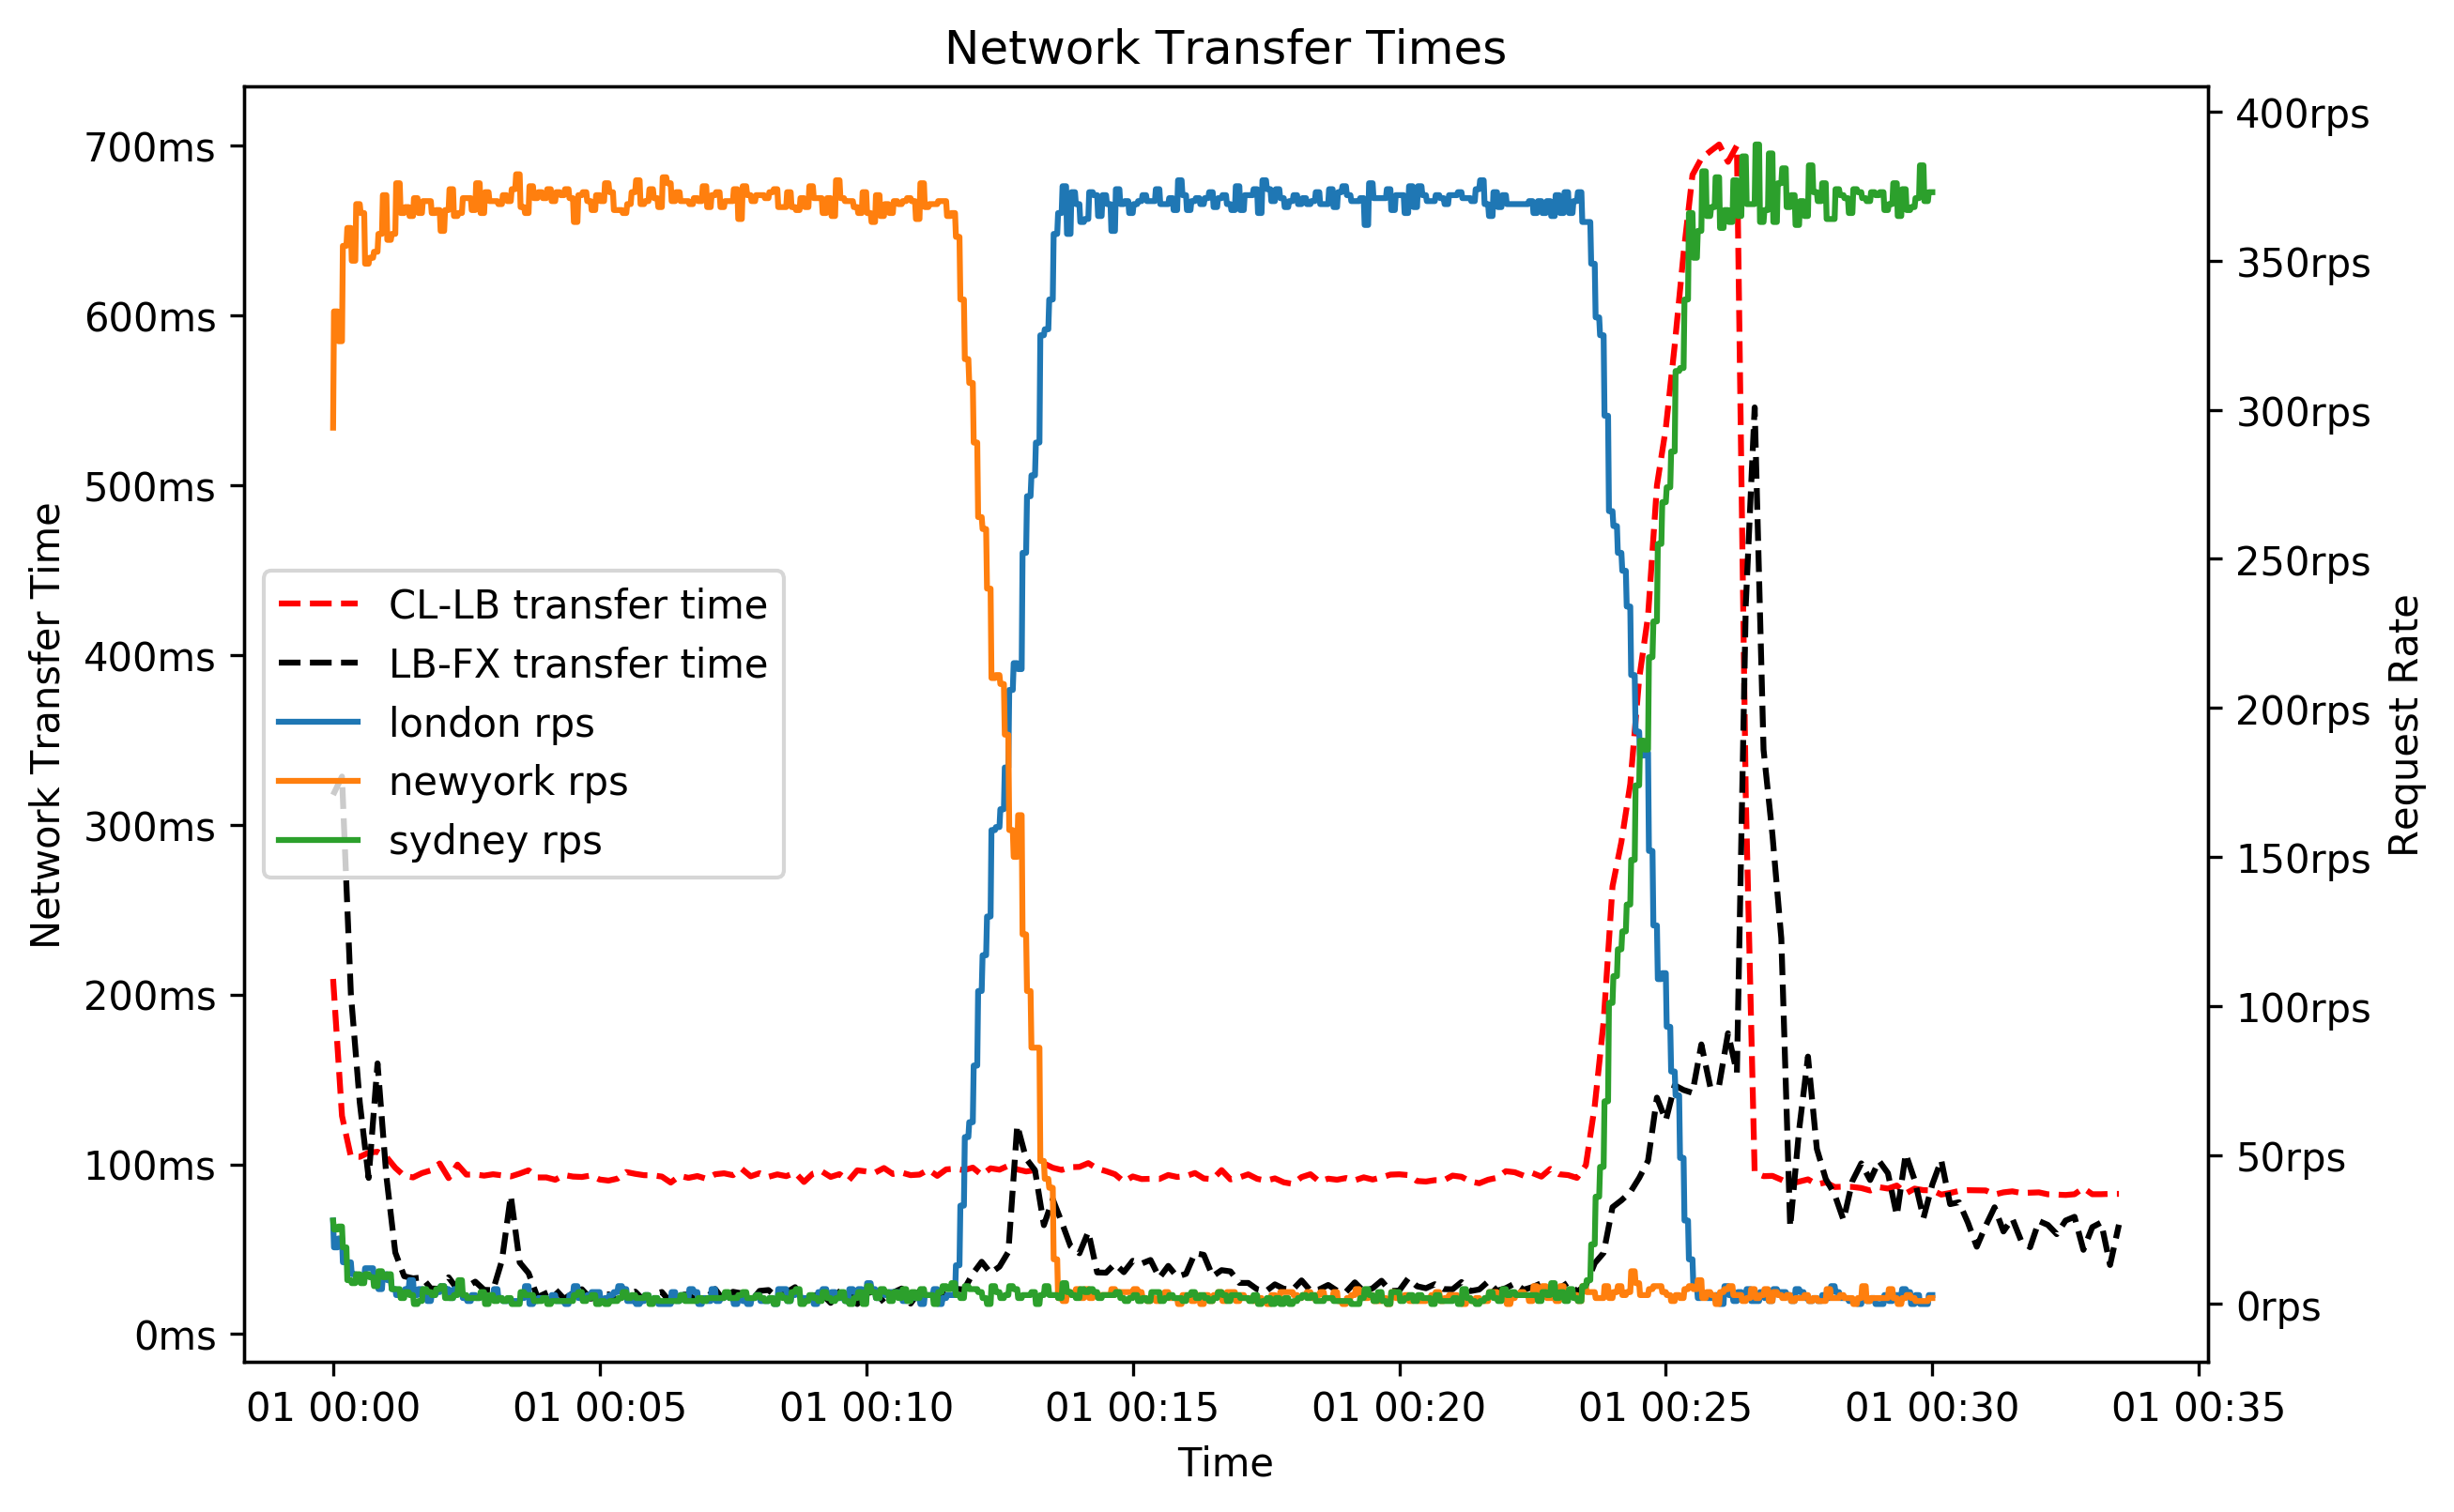
\includegraphics[width=14cm]{graphics/graphs/osmotic_dynamic_region_tx_times.png}
    \caption{\DIFaddFL{Client to load balancer, and load balancer to function transfer times over changing request origins}}
    \label{fig:osmotic_dynamic_tx}
\end{figure}

\DIFadd{First of all, the results show that the osmotic scaling and scheduling component does indeed take the request origin into account when deciding on the number and location of new load balancer replicas.
Figure \ref{fig:osmotic_dynamic_lb_replicas} shows this in action.
While originally load balancers are only spawned in one city, because all requests originate from it, once requests start coming from another city another load balancer instance is deployed in that city.
}

\DIFadd{The effect this has on the system at large can also be observed easily, as Figure \ref{fig:osmotic_dynamic_trt} shows.
Here we can see that while the total response time of the system spikes once requests start to originate from another city, it starts to stabilize and come down to previous levels again once load balancers are present in the new city.
Please note that the \mbox{%DIFAUXCMD
\gls{trt} }\hskip0pt%DIFAUXCMD
values shown in Figure \ref{fig:osmotic_dynamic_trt} are a moving average over a 10 second window, since this removes noise from the plot, making it more readable.
Likewise the request rate per city in Figures \ref{fig:osmotic_dynamic_lb_replicas}, \ref{fig:osmotic_dynamic_trt}, and \ref{fig:osmotic_dynamic_tx} is a moving average over a 5 second window, and displays the request rate for all functions deployed in the system.
}

\DIFadd{Just like with the \mbox{%DIFAUXCMD
\gls{trt}}\hskip0pt%DIFAUXCMD
, Figure \ref{fig:osmotic_dynamic_tx} shows that the request transfer time between client and load balancer, as well as between load balancer and function replica also spike when traffic originates from a different city.
There too, though we see that it returns to previous levels once load balancer replicas become available near the request origin.
}

%DIF >  phillips: 8-9ish pages
\DIFaddend \chapter{Discussion}

% findings:
% 1) briefly re-state the prelim results
% 2) traefik resource results, nothing special, BUT: respone time increases ram load
% 3) in such a situation, lb placement and information is even more critical, than assumed. i.e. the more sparse close resources the more extreme the rest
% 4) information entropy role, shows clear advantage of entropy -> further justification that we need to schedule efficiently
% 5) weight range can and should be quite large, same with the scaling. Perf spread role in this. Also: results from experiments on which WRR implementation is correct etc.
% 6) ????



% 1) Prelims
% 2) traefik resource eval
% 3) more realistic topo
% 4) load balancer count testsPrel
% 5) LB hyperparameter tests
% 6) the osmotic stuffs?

\DIFdelbegin %DIFDELCMD < \newpage %%%
\DIFdelend \section{Load Balancer Implementation and Parametrization}
% 2-3 pages
% if I need more length I could re-state the implications of the initial evaluation here (if that's necessary only though)
\subsection{Choosing the right implementation}
Our evaluations show that careful consideration is necesssary when deciding on a load balancer implementation.
Our results show that some implementations can exhibit idiosyncratic behaviour that might be undesirable for the FaaS system in general.

Our implementation considerations were focused in large parts on how the weighted round robin component of our approach is implemented.
A key result is that the implementation strongly affects how quickly the load balancer is able to discover enough nodes to make an informed load balancing decision and thus converge onto a somewhat stable response time.
From the results we also learn that a deterministic weighted round robin implementation results in faster discovery of the available nodes, as can also be seen in figure \ref{fig:lb_imp_upstream_coverage}.
The potential difficulty of load balancers discovering nodes in an acceptable time frame in system with very high numbers of nodes or load balancers also supports our decision to already initialize load balancers with weights of neighboring instances to reduce the time until performance stabilizes.

We can also observe that certain implementations may exhibit behaviour that is specific to heterogeneous edge computing environments.
An example of such behaviour is the oscillating performance of the \textit{Adapted Classic} load balancing implementation that can be seen in figure \ref{fig:lb_imp_rt_convergence}.
In this implementation upstreams are always worked through iteratively with faster upstreams being chosen first, before slower upstreams are steadily interleaved in order of their respective weight.
As a result the performance varies with time going through periods where performance is extremely  good, and ones where performance is comparatively poor.
When taking the mean response times over a longer period of time though this implementation performs no worse than the \textit{smooth} implementation we chose for our approach.

While intuitively this behaviour might seem undesirable, it also shows potential for more complex application scenarios.
A load balancer could, for example, try to sample as many upstreams as possible, but only send requests to a certain percentile of the best performing ones.
This approach is similar to the implementation proposed by Cicconetti, Conti, and Passarella \cite{cicconettiDecentralizedFrameworkServerless2020}, where they propose to only include upstreams whose response time is at most double the minimum response time achieved.
Sampling in their approach is handled through a generally fixed rate, but with the addition of exponential back off times for upstreams that continuously fail to make the cut.

In terms of additional features, the stratification of upstreams according to their performance would, for example, allow client-specific \gls{qos} policies to be enforced.
This could be relevant for scenarios where some requests are urgent, while others are not, or where devices have to compete for and bid on their \gls{qos}.

Our results here show that there isn't necessarily a singular, optimal implementation, but that depending on goals and requirements of the system an implementation should be chosen.
It also shows, once again, that even system components as basic as weighted round robin implementations may behave differently in a heterogeneous environment such as edge computing, and that careful evaluations are necessary when reusing components developed for the cloud at the edge.

\subsection{Choices in parametrization}
Parametrization is another area where our results indicate developers can make a choice.
As figures \ref{fig:lb_hyper_scaling_perfspread} and \ref{fig:lb_hyper_weightrange_scaling} show, the choice of parameters for how and when response times are mapped onto weights has a significant impact on response times.
The results show that for any given scenario, there can be a whole set of different configurations that would results in the same performance.
We can, however, also see that parameter choices are not universally wise.
What results in good performance under one set of circumstances can result in poor performance under another.
Figure \ref{fig:lb_hyper_reset_q95} shows this well.
While the configuration with weight updates every 150-200 seconds, and a weight range of 20-30 performs well in the 95th percentile in the range of up to 250 \gls{rps}, once \gls{rps} go beyond 500, it performs much worse.

Because \gls{rps} changes are to be expected in a serverless edge computing system, these results indicate that load balancers potentially have to dynamically adapt their parametrization to keep performance as high as possible.
Our results also show that the higher the \gls{rps} a load balancer experiences, the smaller the set of configurations with near optimal performance becomes.
This is particularly relevant to scenarios with high load and strict \gls{sla} policies, since those circumstances would be most affected by suddenly worsened performance due to high \gls{rps} numbers.
While our experimentation in this area is not extensive enough to arrive at definitive conclusions, it suggests that scenarios in which \gls{rps} varies highly requires very careful investigation of the impact of parametrization.


% large effect of parametrization fig 6.5
% interestingly optimal parametrization not static
% depending on scenario performance will vary -> rps is one such variable! likely to change
% again potential for QoS things
%DIF <  the higher the rps the fewer good configurations there are -> the stakes are higher \newpage 
 \DIFdelbegin %DIFDELCMD < \newpage %%%
\DIFdelend %DIF >  the higher the rps the fewer good configurations there are -> the stakes are higher
\section{Resource Usage and Load Balancer Scale}
% 1 page
\subsection{Resource Usage Patterns}
Somewhat unexpectedly, the resource usage between different device types differs significantly.
While the variance in CPU utilization was to be expected, given that the different device's processors vary vastly in terms of core count, frequency, cache size, and power consumption, the difference observed in terms of memory consumption is harder to explain.

As can be seen in table \ref{tab:resource_eval_results}, the memory consumption is split in two groups which differ by a factor of four. Considering that there groups aren't separated by the device's respective processor architecture, we believe that operating system specific reasons are the cause of these variations.
While all devices tested run some form of Linux, typically Debian based, the specific Linux distribution differs, because particularly the edge-type devices feature special purpose hardware and thus rely on specially adapted version of Linux to function properly.

We also observe that the edge devices more frequently feature ARM based processor architectures, which are lower in computational power and for which running a load balancer instances poses a bigger challenge compared to traditional x86 based systems. One should note, however, that this different is not necessarily due to the processor architecture itself, but due to the fact that the devices feature very different \glspl{tdp}, and ARM based devices feature lower \glspl{tdp}, at least in the selection of devices we evaluated.

The second major observation of this experiment, namely that longer response times or upstream node lead to increased memory usage as can be seen in figure \ref{fig:lb_resources_by_rt}, is  easily explained.
As the type of load balancer we evaluate is an application level load balancer, when receiving a request it must first fully receive it before it can make a load balancing decision.
This means that if a request takes longer to receive its parts need to be kept in memory for a longer time.
This is true both for clients sending requests, as well as for upstreams responding to forwarded requests.
This also holds for the request processing time, or \gls{fet} in serverless computing, as the load balancer needs to at least keep some information of each request in memory while the upstream processes it.




% Todo put this in the discussion
% This effect is also due to the reason that not all nodes have clients close to them, which means that while there are more load balancers present in the system, the number of load balancers actually receiving traffic from clients doesn't change, as clients send traffic to the closest load balancer.
% We can also show this in the data -> e.g. global high: 50% -> 90 load balancers in use, 100% -> 113 load balancers in use.
\subsection{Load Balancer Scale}
Our results show that the scale of load balancers in the system has a significant effect on the system's performance.
Particularly at the beginning, when the system's load balancers still have to evaluate the performance of each upstream, different scales perform differently.
Naively speaking, lower numbers of load balancers perform better early on, because they converge to a stable response time sooner, but larger numbers perform better later on, because they tend to be more spread out and thus possess more optimization potential.

While adding more load balancers to the system generally improves the maximum achievable performance, the returns diminish beyond a certain point, as can been seen in the evaluation results in table \ref{tab:lb_scaling_converged_trt}.
This effect is also due to the reason that not all nodes have clients close to them, which means that while there are more load balancers present in the system, the number of load balancers actually receiving traffic from clients doesn't change, as clients send traffic to the closest load balancer.
In our globally distributed evaluation topology with roughly 400 nodes and 75 \gls{rps}, for example, 50\% of nodes hosting load balancers (i.e. ~200 load balancers) results in 90 load balancers actually being used by clients. Doubling this number to 100\% of nodes hosting load balancers, only results in 113 load balancer instances actually being used.
This makes it clear that not only is there a certain number of load balancers beyond which performance improvements diminish significantly, it also shows that this point is dependent on the location of load balancers in the system.

\subsection{Implications}
The results of our evaluation of both resource consumption and load balancer scale have a number of implications for the design decisions of serverless edge computing systems in regard to how load balancing is handled.

First, we have to assume that for each load balancer in a Kubernetes based system 128MiB of memory should be requested to allow for a safe headroom in case large requests have to be handled, the request rate peaks, or other issues lead to overhead.
Through the memory consumption, but particularly through the CPU consumption results show that running a load balancer can be a significant task for a smaller, edge-based device.

Secondly, these results make it clear that load balancers need to be scaled and scheduled in a more sophisticated way than is default in Kubernetes and thus in most existing serverless systems.\\
After a certain point, adding more load balancers yields to massively diminishing returns, making the addition of more inefficient from a resource perspective.
At which point more load balancers become inefficient depends on the system's priorities and capabilities, and the scaling component is what should continuously evaluate this question.
The efficiency of the load balancers that are present in the system depends on their location, since a load balancer that receives no traffic is essentially a waste of resources, just as one that receives a lot of traffic, but is located far from clients or upstreams, results in overly distant network transfers.
This makes the effective placement of load balancers in the system a key component of minimizing the number of load balancer instances needed, and thus the amount of resources consumed.\\
Particularly at the edge, where resources can potentially be scarce and valuable, this makes a strong case for new scaling and scheduling methods such as the one we present in this thesis.

Lastly, the results of our evaluation show that the number of load balancers in the system can actively be used as a variable to influence the overall performance achieved.
This potentially gives developers the flexibility to make an informed trade off between the amount of resources consumed by load balancers, and the resulting performance.
Through this more fine grained control over the system's \gls{qos} could be achieved, and differentiated policies developed to guarantee performance levels compliant with different levels of \gls{sla}.
\DIFdelbegin %DIFDELCMD < \newpage 
%DIFDELCMD <  \newpage %%%
\DIFdelend \DIFaddbegin 

\DIFaddend \section{\DIFdelbegin \DIFdel{Impact of }\DIFdelend Osmotic Scaling and Scheduling}
%DIF <  2 pages \newpage 
 \DIFdelbegin %DIFDELCMD < \newpage %%%
\DIFdelend %DIF >  2 pages
\DIFaddbegin 

\subsection{\DIFadd{Basic Evaluation}}
\DIFadd{From the basic evaluation of how our proposed osmotic scaling and scheduling approach performs we can make a number of important observations.
First and foremost we see that our approach does indeed work and correctly scales up to at least one load balancer replica per city and schedules these replicas.
Using similarly low load balancer replica counts with a random scheduling method would likely result in much worse performance, as there would be a significant chance of a city not having an instance deployed.
This demonstrates how the location aware components of the scheduler successfully identify areas where a significant share of requests originates from and then starts the load balancer replica there, while also taking into account the locations of the required upstream functions.
}

\DIFadd{We can, however, also see from table \ref{tab:osmotic_base} that the osmotic approach doesn't always behave consistently in all scenarios.
In the city topology based scenarios the osmotic scaler consistently deploys many more load balancers than in other scenarios.
While this comparatively high replica count results in good performance, the fact that the same scaling and scheduling configuration results in different scaling decisions and levels based on topology highlights that there is no single set of optimal parameters.
How the scaler is configured and which parameters are right will depend on the level of performance required of the load balancers, and the node topology of the system in question.
}

\DIFadd{What this finding suggests is that for our approach to work in a larger variety of network topologies irrespective of scale we may have to change the way in which osmotic pressure is calculated.
Currently absolute information with regard to the size of the system is not included at all, as our calculations purely rely on metrics' magnitude relative to each other.
Right now the size of the system in question is implicitly encoded in the set pressure thresholds.}\\
\DIFadd{An example might help to illustrate this more clearly: Assuming a network needs a fixed number of load balancers positioned well in order to achieve a certain performance level.
If we now have a suitable pressure level to achieve the performance in question, and want to find the configuration for a system many times that size we know that for the larger system overall more load balancers will be required.
Because the pressure computations themselves work irrespective of the system size, what needs to change is the threshold at which load balancer replicas are scaled up. }\\
\DIFadd{In the interest of stabilizing load balancer performance resulting from scaling and scheduling decisions one would need to take a closer look into the relationship between the parametrization,  the make-up of the system, and the resulting performance.
}

\DIFadd{What we could show with these initial experiments is that our osmotic approach is capable of providing tangible performance benefits over the status-quo of serverless edge computing frameworks, although some manual tuning of the configuration is necessary to achieve the best performance possible.
}

\subsection{\DIFadd{Optimization Aggressiveness}}
\DIFadd{The basic evaluation of our osmotic approach and the load balancer scale experiment already showed how larger numbers of load balancers tend to result in better system performance, and the performance results of this experiment are right in line with the previous findings.
Knowing this, the question is how our proposed osmotic scaling and scheduling approach influences the scale, and thus the performance.
}

\DIFadd{As discussed, the primary way the number of load balancers in the system can be influenced is via the pressure thresholds, with lower thresholds resulting in higher replica counts.
The experiment shows this behaviour clearly, with the lower thresholds indeed resulting in higher replica counts.
By just how much these thresholds influence the replica counts isn't intuitively obvious though, and as we can see in table \ref{tab:osmotic_scaling_aggressiveness}, the relationship between the threshold and resulting scale is not linear.
Because the benefits of increasing the amount of load balancer replicas themselves aren't linear either, the results indicate that the tuning of the pressure threshold parameters to meet certain performance criteria is a complex task.
}

\DIFadd{It opens up a more general question of how the configuration complexity in serverless edge computing should be addressed.
In real deployments there is the potential of strict \mbox{%DIFAUXCMD
\gls{sla} }\hskip0pt%DIFAUXCMD
requirements for certain functions, which creates the need to predict the system performance based on its topology and parameter configuration.
Perhaps the way to deal with this complexity is not a systematic evaluation of topologies,  configuration parameters, and their interplay, but rather an agent that dynamically adjusts parameters based on current performance and requirements.
If performance is insufficient and the workload in question is network bound, 
this agent could then for example decrease the pressure threshold to spawn more load balancers.
%DIF >  for baseline:
%DIF >  lb replica count correlated to osmotic
%DIF >  shows some limitations of osmotic in that it's not super consistent between city and nation
%DIF >  osmotic seems to be pretty efficient -> we couldn't even try lower random scales b.c. of network flow congestion and the simulation then not terminating anymore
}


%DIF >  for optimization aggressiveness
%DIF >  could be used to derive load balancer scale for certain SLAs
%DIF >  not exactly easy to derive a parametrization for a target SLA though, it's more like a continuous adjustment until you arrive at the target parametrization
%DIF >  higher scales and their resource costs need to be weighed against the benefits -> This is especially true when some node's resources are more precious than another's -> think something is highly specialized AI hardware and the other is just something generic. With the AI blocking that memory and compute is comparatively "expensive"


\subsection{\DIFadd{Dynamic System Conditions}}
\DIFadd{One of the core motivations for our osmotic approach is the necessity for the scaling and scheduling component to adapt to changing system conditions, and in particular to system conditions which are not known beforehand.
One of these system conditions is which part of the system requests originate from.
}

\DIFadd{Ideally, the osmotic scaling and scheduling component should register rising pressure once requests come from an area where no load balancer is close-by and then schedule one to be deployed there.
From the results of the experiment we can see that our approach reacts exactly in this way, scaling up and scheduling replicas in each of the cities once requests start originating from there in significant numbers.
Figure \ref{fig:osmotic_dynamic_lb_replicas} shows this behaviour visually, with load balancer replica counts rising shortly after request rates rise.
}

\DIFadd{While our approach does react to the changing request origin correctly, there are still some points that could be improved.
First of all, once the origin changes we can still observe a significant spike in response time as is also shown by figure \ref{fig:osmotic_dynamic_trt}.
In the experiment the request origin changes from one city to the other such that each city is the main request origin at one point.
Although when requests change origin for the first point the spike in \mbox{%DIFAUXCMD
\gls{trt} }\hskip0pt%DIFAUXCMD
is comparatively small, going from a baseline of around 140ms to 250ms, the temporary decrease in performance is much more pronounced on the second change, spiking up to 380ms.
The reason the first spike is so small in comparison is that in the second city already has a load balancer replica deployed.
Like we describe in our approach, there has to be at least one load balancer present in the system at all times for requests to be processed at all. 
In this case the load balancer happened to initially be deployed in the second city, shortening the time until response times stabilized again.
}

\DIFadd{There are a number of factors that influence how quickly the system adapts to changes in request origin: The rate at which the system evaluates the osmotic pressure, how quickly a load balancer can be deployed on the selected node, and how quickly the load balancer gathers sufficient information to make informed load balancing decisions.
The last point in particular, how quickly the new load balancer makes effective decision, can take more or less time depending on how much traffic the new load balancer receives and how well the initial values fit for the location and traffic of the new instance.
}

\DIFadd{Our evaluation also showed some limitations of our approach.
For extreme cases like the scenario tested in this experiment the de-scheduling portion of our approach does not work as well.
Since our approach is not based on any a-priori information on the system, and uses the expected relative performance improvement when deciding on whether or not to de-schedule a load balancer, it can sometimes keep instances that are no longer needed.
Because a load balancer running even though there is little traffic in an area does not deteriorate the system's performance in terms of \mbox{%DIFAUXCMD
\gls{trt}}\hskip0pt%DIFAUXCMD
, the scaler cannot detect a probable performance improvement from de-scheduling and thus leaves the instance running. 
This is also visible in the results of this experiment.
Figure \ref{fig:osmotic_dynamic_lb_replicas} shows how load balancers scale up once requests originate from a new city, but it also shows how the previously scheduled load balancers remain, even though the request share they receive is miniscule compared to the newly scheduled instances.
}


%DIF >  for dynamic system
%DIF >  current limitation: downscaling when there is too little traffic. Currently just not really supported, as removing a LB with no traffic also doesn't improve performance.
%DIF >  there is a bit of a delay since first the scaling logic needs to run, and it then takes a bit for the load balancer to be A) deployed and B) converge on decent weights for good upstream performance. Also for C) the approach of initializing with the next closest LB values can also work against us if that LB is farther away an it's configuration would be poor for our case
%DIF > also mention that since london has the seed-load balancer the spike there is relatively speaking pretty small.


\DIFaddend \section{Implications of Osmotic Scaling for Serverless Edge Computing}
%DIF <  2-3 pages \newpage 
%DIF >  2-3 pages
\DIFaddbegin 

\DIFadd{Finally we have to ask what implications our approach and the general idea of osmotic scaling and scheduling have for the area of serverless edge computing.
Osmotic computing has been proposed as a potential solution to provide an effective solution to the complex task of cloud-edge integration\mbox{%DIFAUXCMD
\cite{osmotic-middleware-rausch}}\hskip0pt%DIFAUXCMD
.
Specifically it provides a promising approach for dealing with changing system conditions, and environments which are not known beforehand.
Our experiments suggest that withing the area of serverless computing, particularly for scaling and scheduling load balancers, osmotic approaches offer tangible benefits.
Our evaluations show that an osmotic approach allows us to react to changing system conditions well, and that even though the environment is unknown beforehand ,comparatively decent scaling and scheduling decisions can be made that result not only in better performance than current serverless solutions offer at the edge, but also increased resource efficiency through reduced scales.
}

\DIFadd{Our evaluations also show however, that our approach does not yet provide a solution that fits every serverless edge computing scenario and use-case.
While the design of our approach aims to rely as little as possible on a-priori information about the system, the results of our evaluations show that in certain cases this type of a-priori knowledge is required to have consistent behaviour in different scenarios. 
The size of the system, for example, is one such factor that needs to be known beforehand so that the scaling and scheduling parameters can be set in a way that the system performs according to the scenario's requirements.
}

\DIFadd{This inherent challenge between a need for a-priori information about the system on one hand, but edge computing systems being dynamic and thus changing in nature on the other suggests that a static parameter choice might never work in a sufficiently predictable way.
Instead, a self-adapting system that tunes the parameters of the system in real time might result in more predictable behaviour across more scenarios.
}

\DIFadd{In addition to the topics explicitly tested in the experiments we would like to briefly outline other aspects of osmotic scaling and scheduling for serverless edge computing that should be investigated prior to real-world deployment.}\\
\DIFadd{First, it might be beneficial to create a simplified heuristic version of the pressure calculation. Depending on the size of the serverless system, the computational effort to perform these calculations in short intervals could start to be a limiting factor on how quickly the scaler and scheduler can react to changes in the system.
This would be particularly true of highly dynamic scenarios, as these make solutions such as caching and re-using certain parts of the computation infeasible.}\\
\DIFadd{Second, our approach does not yet include one of the potentially most important aspects of serverless edge computing: Different priority and \mbox{%DIFAUXCMD
\gls{qos} }\hskip0pt%DIFAUXCMD
levels.
With the heterogeneous nature of edge computing scenarios also come additional challenges for providing certain \mbox{%DIFAUXCMD
\gls{qos} }\hskip0pt%DIFAUXCMD
levels.
In edge computing, certain resources might be more precious than others and effective usage is required to achieve the best performance possible.
For our osmotic scheduling approach this means that these kinds of priorities and goals will need to be included in the pressure calculation, if the scaling and scheduling of the system should take them into account.
}

\DIFaddend % target: 4ish pages
\DIFaddbegin 

%DIF >  Philipps DA: 1p intro, 1p per RQ, 1p future work
\DIFaddend \chapter{Conclusion}
\DIFdelbegin %DIFDELCMD < \newpage %%%
\DIFdelend \DIFaddbegin \DIFadd{Edge computing has been proposed as a new computing paradigm to address the computational needs of new applications such as real-time cognitive assistance, large scale analytics from \mbox{%DIFAUXCMD
\gls{iot} }\hskip0pt%DIFAUXCMD
sensors, or deep learning based image analysis on resource constrained devices.
Edge computing brings with it a number of significant implementation challenges.
In particular, edge computing environments are heterogeneous in hardware, software and networking conditions, featuring drastically different hardware, various operating systems, and a wide range of network conditions.
In addition to the system itself being heterogeneous, the surrounding conditions can be highly dynamic with request rates, clients, running applications, and the very structure of the system changing over time, in some scenarios even very quickly.
}

\DIFadd{Currently, this complexity needs to be resolved by system developers themselves, which is not only very difficult, but is typically implementation-specific and thus not efficient in the long run.
Serverless computing has been proposed as an abstraction layer on top of edge computing systems with the goal of alleviating the need to deal with this complexity for developers.
Instead, the serverless edge computing framework is supposed to handle the tasks of scheduling and scaling functions, as well as routing them in such a way that the requirements of the application are fulfilled.
While serverless systems have been adapted to be edge-capable, there are some challenges that remain.
Network bound workloads in particular are an area where the performance of serverless edge computing systems was not in line with expectations.
}

\DIFadd{This is the area of serverless edge computing this work aims to improve upon.
We perform an initial analysis of the load balancing component of the serverless system, which we suspect is the key component that needs to be adapted for network bound workloads to perform better.
Based on these results we propose to improve load balancing for serverless edge computing through two adaptations.
First, our approach changes the operating logic of the load balancer itself, moving away from the simple round robin load balancing current systems default to, towards a weighted response time implementation that tunes and adapts weights dynamically based on a least response time logic.
Second, we propose an osmotic pressure based approach to scaling and scheduling load balancer replicas, giving load balancers their own scaling and scheduling logic separate from the one regular serverless functions use, which allows the load balancer scheduling to consider the location of both function replicas and clients.
}

\DIFadd{Results show that our approach not only significantly improves response times of network bound workloads, but that it also opens up future opportunities for sophisticated deployment scenarios that have more differentiated performance requirements.
}

\DIFaddend \section{Research Questions}
\DIFdelbegin %DIFDELCMD < \newpage 
%DIFDELCMD <  \newpage %%%
\DIFdelend \DIFaddbegin 

\subsubsection{\DIFadd{How can current scaling, placement, and routing techniques for load balancers be changed, such that the overall performance of the serverless edge computing system improves?}}

\DIFadd{In their current state serverless edge computing systems treat load balancers as "just another function", not paying special attention to how they are scheduled and scaled.
Likewise the routing (i.e. load balancing) decisions themselves are made by algorithms designed for and tested in cloud-centric environments.
To improve performance, both of these areas have to be adapted to deal with the challenges of the edge computing environment.}\\
\DIFadd{To improve routing decisions we move away from simple round robin load balancing, which is incapable of addressing the heterogeneous device capabilities found in edge computing.
Instead we use a variant of weighted round robin load balancing, which is better suited to deal with the differently performant devices and accordingly differently performant upstreams.
Because the performance of different devices is not known beforehand, and can change dynamically at runtime we use the observed response time of past requests as a black box metric and stand in for the expected performance of the upstream in question.
Based on a moving average of these past response times and a least response time logic we assign each of the upstreams their respective weights used by weighted round robin.
This evaluation of observed response times and weight mappings happens continuously and as a result it can adapt to changing system conditions as well.
For scaling and scheduling we introduce an approach inspired by the concept of osmotic pressure we call osmotic scaling and scheduling.}\\
\DIFadd{The load balancer scaling and scheduling component needs to take into account where in the network client requests are originating from, where function replicas to handle those requests are located, and where load balancer instances are already present.
To this end we introduce the notion of osmotic pressure.
For each node that does not already have a load balancer deployed, we calculate a pressure metric that depends on how many requests it would receive if there was a load balancer present, how close the clients sending these requests are, and how close the function replicas required to process the requests are located.
If the pressure exceeds a set threshold a new load balancer replica is added on that node.
Likewise a negative pressure is calculated for nodes which are already host to a load balancer instance, where requests that would be more efficiently handled by other running load balancer instances contribute to negative pressure.
If the pressure falls below the downscaling pressure threshold the load balancer replica is removed.}\\
\DIFadd{Through the introduction of these techniques for load balancing, scaling and scheduling the overall performance of the system improves, particularly for network bound workloads.
}


\subsubsection{\DIFadd{How much of a performance improvement can be gained from optimizing the scaling, placement and decisions of load balancers in serverless edge computing systems?}}

\DIFadd{Our initial evaluations show that the diagnosis of load balancer location and load balancing technique was correct.
In the first evaluation, where we tested the new load balancing implementation and compared a scenario with a centralized round robin load balancer on one hand, and our adapted version running on every node on the other, the mean total response time could be improved by between 81\% and 606\%, depending on the scenario.
These performance gains hold, albeit in a less dramatic way in our more stringent and realistic evaluation of the osmotic scaling and scheduling component.
In these tests the results still show an improvement between in mean \mbox{%DIFAUXCMD
\gls{trt} }\hskip0pt%DIFAUXCMD
between 43\% and 229\% compared to a non-centralized round robin implementation, which corresponds to a reduction of -30\% to -69\% in \mbox{%DIFAUXCMD
\gls{trt}}\hskip0pt%DIFAUXCMD
.
The improvements are larger when looking not only at the mean values, but at the different percentiles as well.}\\
\DIFadd{The higher the percentile, the bigger the \mbox{%DIFAUXCMD
\gls{trt} }\hskip0pt%DIFAUXCMD
improvement generally is.
What this means is that our approach not only improves the performance of the system on average, it also reduces the variance, making the performance gains more reliable.
The performance gains are realized by having decreased network transfer times between client and load balancer, and load balancer and function replica.
This is expected and optimizing this part of the response time is the primary implementation goal of the osmotic scaling and scheduling approach we present.
In addition to improving network transfer times, our approach realizes part of its performance gains via improvements \mbox{%DIFAUXCMD
\gls{fet}}\hskip0pt%DIFAUXCMD
, which are a result of the load balancing implementation relying on a black box metric that also encompasses \mbox{%DIFAUXCMD
\gls{fet} }\hskip0pt%DIFAUXCMD
and thus partially optimizing for it.
}

\subsubsection{\DIFadd{How do edge optimized scaling and placement techniques for load balancers, including the load balancing techniques themselves, affect the overall system behaviour
and characteristics in regard to their key performance metrics?}}

\DIFadd{Our approach also has effects on the system beyond its improvements in \mbox{%DIFAUXCMD
\gls{trt}}\hskip0pt%DIFAUXCMD
.
Notably it positions load balancers efficiently, achieving performance that would require the deployment of more load balancer instances when using current scheduling methods.
This is particularly relevant as our experiments with real hardware show that depending on the device and operating system used memory and CPU consumption can vary significantly.}\\
\DIFadd{In addition we can observe that our approach slightly reduces the number of function replicas deployed in the serverless system, when using the default scaling methodology of OpenFaaS\mbox{%DIFAUXCMD
\cite{openfaas} }\hskip0pt%DIFAUXCMD
as a representative example of serverless frameworks in general.
While these reductions in function scale are too small to be considered a stable feature of our approach, it indicates that it can likely be integrated into serverless frameworks without adverse effect on function scale.}\\
\DIFadd{As one would expect based on the faster network transfer times, our approach reduces the share of requests that get routed to far-away function replicas.
In an evaluation with three distinct cities far apart from each other our approach routes only 1.9\% of requests to a function replica outside the city, compared to the 65.2\% of round robin based load balancing currently used in serverless frameworks.
}\DIFaddend \section{Future Work}
\DIFdelbegin %DIFDELCMD < \newpage 
%DIFDELCMD < %%%
\DIFdelend \DIFaddbegin 

%DIF >  future work idea: it is relatively obvious that there is a non-linear relationship between load balancer scale and the performance limit they provide. The question now is how the linearity and scales here are influenced by the network itself. Can there, based on the network structure, be a way to determine the "optimal" number, or predict the impact sufficiently accurately that one can derive the "correct" scale given certain SLA requirements?

%DIF >  how does information sharing between load balancerns contribute to their performance, and how can this be solved on an engineering-level to avoid exponential growth in data transfer sizes? also: how would the stochastic congestion game idea factor into this?

\DIFadd{Our work provides a basis on which future work can be built, both to address limitations of our approach, as well as to further the capabilities of serverless edge computing.
This section provides a list of some of the most important areas for future work.
}\begin{itemize}
    \item \DIFadd{A continued evaluation of our approach in different deployment scenarios and network topologies could give further insight into its advantages and limitations. Based on this our approach could be changed to bring it closer to a state where it can reliably be used in real-world deployments.
    }\item \DIFadd{Building on our results, that show how response time percentiles and general service levels are influenced by load balancer scaling and implementation, a more sophisticated approach could be developed that takes into account and optimizes for different \mbox{%DIFAUXCMD
\gls{qos} }\hskip0pt%DIFAUXCMD
levels on a per-function basis.
    }\item \DIFadd{In keeping with the previous point about different \mbox{%DIFAUXCMD
\gls{qos} }\hskip0pt%DIFAUXCMD
levels, our approach could be modified to explicitly model the requirements of functions and then automatically tune its parameters accordingly. This would stand in contrast to current, statically configured implementations. In addition the need to do so is indicated by our experimental results, which show that for different environments different configurations are required to achieve optimal performance.
    }\item \DIFadd{Joint scheduling and scaling of functions and load balancers offers the potential for additional performance gains, where the information about required resources gathered by the load balancer could help make more informed decisions about function replica scale and location.
    }\item \DIFadd{Lastly, the topic of standardized edge computing scenarios for benchmarking remains a worthwhile area to improve upon. While there is effort to develop systematic benchmarks for edge computing, for example EdgeBench\mbox{%DIFAUXCMD
\cite{edgebench}}\hskip0pt%DIFAUXCMD
, there is much to be done in terms of modelling network topologies and dynamically changing environments. Such a suite of standardized benchmarks and deployment scenarios would help to make competing approaches more directly comparable, and results more transparent.
    }

\end{itemize}   
\DIFaddend % \chapter{Introduction}
% \todo{Enter your text here.}

% \chapter{Additional Chapter}
% \todo{Enter your text here.}

% Remove following line for the final thesis.
% %% intro.tex
%% Copyright (C) 2014-2020 by Thomas Auzinger <thomas@auzinger.name>
%
% This work may be distributed and/or modified under the
% conditions of the LaTeX Project Public License, either version 1.3
% of this license or (at your option) any later version.
% The latest version of this license is in
%   http://www.latex-project.org/lppl.txt
% and version 1.3 or later is part of all distributions of LaTeX
% version 2005/12/01 or later.
%
% This work has the LPPL maintenance status `maintained'.
%
% The Current Maintainer of this work is Thomas Auzinger.
%
% This work consists of the files vutinfth.dtx and vutinfth.ins
% and the derived file vutinfth.cls.
% This work also consists of the file intro.tex.


\newacronym{ctan}{CTAN}{Comprehensive TeX Archive Network}
\newacronym{faq}{FAQ}{Frequently Asked Questions}
\newacronym{pdf}{PDF}{Portable Document Format}
\newacronym{svn}{SVN}{Subversion}
\newacronym{wysiwyg}{WYSIWYG}{What You See Is What You Get}

\newglossaryentry{texteditor}
{
  name={editor},
  description={A text editor is a type of program used for editing plain text files.}
}

\chapter{Introduction to \LaTeX}

Since \LaTeX\ is widely used in academia and industry, there exists a plethora of freely accessible introductions to the language.
Reading through the guide at \url{https://en.wikibooks.org/wiki/LaTeX} serves as a comprehensive overview for most of the functionality and is highly recommended before starting with a thesis in \LaTeX.

\section{Installation}

A full \LaTeX\ distribution\index{distribution} consists not only of the binaries that convert the source files to the typeset documents, but also of a wide range of packages and their documentation.
Depending on the operating system, different implementations are available as shown in Table~\ref{tab:distrib}.
\textbf{Due to the large amount of packages that are in everyday use and due to their high interdependence, it is paramount to keep the installed distribution\index{distribution} up to date.}
Otherwise, obscure errors and tedious debugging ensue.

\begin{table}
  \centering
  \begin{tabular}{cccc}
    \toprule
    Distribution & Unix         & Windows      & MacOS        \\
    \midrule
    TeX Live     & \textbf{yes} & yes          & (yes)        \\
    MacTeX       & no           & no           & \textbf{yes} \\
    MikTeX       & (yes)        & \textbf{yes} & yes          \\
    \bottomrule
  \end{tabular}
  \caption{\TeX/\LaTeX\ distributions for different operating systems. Recomended choice in \textbf{bold}.}
  \label{tab:distrib} % \label has to be placed AFTER \caption to produce correct cross-references.
\end{table}

\section{Editors}

A multitude of \TeX\ \glspl{texteditor} are available differing in their editing models, their supported operating systems and their feature sets.
A comprehensive overview of \glspl{texteditor} can be found at the Wikipedia page  \url{https://en.wikipedia.org/wiki/Comparison_of_TeX_editors}.
TeXstudio (\url{http://texstudio.sourceforge.net/}) is recommended.
Most editors support a synchronization of the generated document and the \LaTeX\ source by \verb|Ctrl| clicking either on the source document or the generated document.

\section{Compilation}

Modern editors usually provide the compilation programs to generate \gls{pdf} documents and for most \LaTeX\ source files, this is sufficient.
More advanced \LaTeX\ functionality, such as glossaries and bibliographies, needs additional compilation steps, however.
It is also possible that errors in the compilation process invalidate intermediate files and force subsequent compilation runs to fail.
It is advisable to delete intermediate files (\verb|.aux|, \verb|.bbl|, etc.), if errors occur and persist.
All files that are not generated by the user are automatically regenerated.
To compile the current document, the steps as shown in Table~\ref{tab:compile} have to be taken.


\begin{table}
  \centering
  \begin{tabular}{rl}
    \toprule
    & Description \\
    \midrule
    1 & Scan for refs, toc/lof/lot/loa items and cites \\
    2 & Build the bibliography     \\
    3 & Link refs and build the toc/lof/lot/loa \\
    4 & Link the bibliography \\
    5 & Build the glossary \\
    6 & Build the acronyms \\
    7 & Build the index \\
    8 & Link the glossary, acronyms, and the index \\
    9 & Link the bookmarks \\
    \midrule
    & Command \\
    \midrule
    1 & \verb|pdflatex.exe  example| \\
    2 & \verb|bibtex.exe    example| \\
    3 & \verb|pdflatex.exe  example| \\
    4 & \verb|pdflatex.exe  example| \\
    5 & \verb|makeindex.exe -t example.glg -s example.ist| \\
      & \verb|              -o example.gls example.glo| \\
    6 & \verb|makeindex.exe -t example.alg -s example.ist| \\
      & \verb|              -o example.acr example.acn| \\
    7 & \verb|makeindex.exe -t example.ilg -o example.ind example.idx| \\
    8 & \verb|pdflatex.exe  example| \\
    9 & \verb|pdflatex.exe  example| \\
    \bottomrule
  \end{tabular}
  \caption{Compilation steps for this document. The following abbreviations were used: table of contents (toc), list of figures (lof), list of tables (lot), list of algorithms (loa).}
  \label{tab:compile} % \label has to be placed AFTER \caption to produce correct cross-references.
\end{table}


\section{Basic Functionality}

In this section, various examples are given of the fundamental building blocks used in a thesis.
Many \LaTeX\ commands have a rich set of options that can be supplied as optional arguments.
The documentation of each command should be consulted to get an impression of the full spectrum of its functionality.

\subsection{Floats}

Two main categories of page elements can be differentiated in the usual \LaTeX\ workflow: \textit{(i)} the main stream of text and \textit{(ii)} floating containers that are positioned at convenient positions throughout the document.
In most cases, tables, plots, and images are put into such containers since they are usually positioned at the top or bottom of pages.
These are realized by the two environments \verb|figure| and \verb|table|, which also provide functionality for cross-referencing (see Table~\ref{tab:intro} and Figure~\ref{fig:intro}) and the generation of corresponding entries in the list of figures and the list of tables.
Note that these environments solely act as containers and can be assigned arbitrary content.

\subsection{Tables}

A table in \LaTeX\ is created by using a \verb|tabular| environment or any of its extensions, e.g., \verb|tabularx|.
The commands \verb|\multirow| and \verb|\multicolumn| allow table elements to span multiple rows and columns.

\begin{table}[h] % placement specifier
  \centering
  \begin{tabular}{lll}
    \toprule
    \multicolumn{2}{c}{Position} \\
    \cmidrule{1-2} % partial horizontal rule
    Group & Abbrev & Name \\
    \midrule
    Goalkeeper & GK & Paul Robinson \\
    \midrule
    \multirow{4}{*}{Defenders} & LB & Lucus Radebe \\
                               & DC & Michael Duburry \\
                               & DC & Dominic Matteo \\
                               & RB & Didier Domi \\
    \midrule
    \multirow{3}{*}{Midfielders} & MC & David Batty \\
                                 & MC & Eirik Bakke \\
                                 & MC & Jody Morris \\
    \midrule
    Forward & FW & Jamie McMaster \\
    \midrule
    \multirow{2}{*}{Strikers} & ST & Alan Smith \\
                              & ST & Mark Viduka \\
    \bottomrule
  \end{tabular}
  \caption{Adapted example from the \LaTeX guide at \url{https://en.wikibooks.org/wiki/LaTeX/Tables}. This example uses rules specific to the \texttt{booktabs} package and employs the multi-row functionality of the \texttt{multirow} package.}
  \label{tab:intro} % \label has to be placed AFTER \caption to produce correct cross-references.
\end{table}

\subsection{Images}

An image is added to a document via the \verb|\includegraphics| command as shown in Figure~\ref{fig:intro}.
The \verb|\subcaption| command can be used to reference subfigures, such as Figure~\ref{fig:intro:full width} and~\ref{fig:intro:half width}.

\begin{figure}[h]
  \centering
  \begin{subfigure}[b]{0.45\columnwidth}
    \centering
    
\includegraphics[width=\textwidth]{Logo-schwarz.pdf}
    \subcaption{The header logo at text width.}
    \label{fig:intro:full width}
  \end{subfigure}
  \begin{subfigure}[b]{0.45\columnwidth}
    \centering
    
\includegraphics[width=0.5\textwidth]{Logo-schwarz.pdf}
    \subcaption{The header logo at half the text width.}
    \label{fig:intro:half width}
  \end{subfigure}
  \caption[Optional caption for the figure list (often used to abbreviate long captions)]{The header logo at different sizes.} % Remove the [...] argument if the original caption should be used in the figure list.
  \label{fig:intro} % \label has to be placed AFTER \caption (or \subcaption) to produce correct cross-references.
\end{figure}

\subsection{Mathematical Expressions}

One of the original motivation to create the \TeX\ system was the need for mathematical typesetting.
To this day, \LaTeX\ is the preferred system to write math-heavy documents and a wide variety of functions aids the author in this task.
A mathematical expression can be inserted inline as $\sum_{n=1}^{\infty} \frac{1}{n^2} = \frac{\pi^2}{6}$ outside of the text stream as \[ \sum_{n=1}^{\infty} \frac{1}{n^2} = \frac{\pi^2}{6} \] or as numbered equation with
\begin{equation}
\sum_{n=1}^{\infty} \frac{1}{n^2} = \frac{\pi^2}{6}.
\end{equation}

\subsection{Pseudo Code}

The presentation of algorithms can be achieved with various packages; the most popular are \verb|algorithmic|, \verb|algorithm2e|, \verb|algorithmicx|, or \verb|algpseudocode|.
An overview is given at \url{https://tex.stackexchange.com/questions/229355}.
An example of the use of the \verb|alogrithm2e| package is given with Algorithm~\ref{alg:gauss-seidel}.

\begin{algorithm}
  \SetKw{BreakFor}{break for}
  \KwIn{A scalar~$\epsilon$, a matrix $\mathbf{A} = (a_{ij})$, a vector $\vec{b}$, and an initial vector $\vec{x}^{(0)}$}
  \KwOut{$\vec{x}^{(n)}$ with $\mathbf{A} \vec{x}^{(n)} \approx \vec{b}$}
  \For{$k\leftarrow 1$ \KwTo maximum iterations}
  {
     \For{$i\leftarrow 1$ \KwTo $n$}
     {
        $x_i^{(k)} = \frac{1}{a_{ii}} \left(b_i-\sum_{j<i} a_{ij} x_j^{(k)} - \sum_{j>i} a_{ij} x_j^{(k-1)} \right)$\;
     }
     \If{$\lvert\vec{x}^{(k)}-\vec{x}^{(k-1)}\rvert < \epsilon$}
     {\BreakFor\;}
  }
  \Return{$\vec{x}^{(k)}$\;}
  \caption{Gauss-Seidel}
  \label{alg:gauss-seidel} % \label has to be placed AFTER \caption to produce correct cross-references.
\end{algorithm}

\section{Bibliography}

The referencing of prior work is a fundamental requirement of academic writing and well supported by \LaTeX.
The \textsc{Bib}\TeX\ reference management software is the most commonly used system for this purpose.
Using the \verb|\cite| command, it is possible to reference entries in a \verb|.bib| file out of the text stream, e.g., as~\cite{Turing1936}.
The generation of the formatted bibliography needs a separate execution of \verb|bibtex.exe| (see Table~\ref{tab:compile}).

\section{Table of Contents}

The table of contents is automatically built by successive runs of the compilation, e.g., of \verb|pdflatex.exe|.
The command \verb|\setsecnumdepth| allows the specification of the depth of the table of contents and additional entries can be added to the table of contents using \verb|\addcontentsline|.
The starred versions of the sectioning commands, i.e., \verb|\chapter*|, \verb|\section*|, etc., remove the corresponding entry from the table of contents.

\section{Acronyms / Glossary / Index}

The list of acronyms, the glossary, and the index need to be built with a separate execution of \verb|makeindex| (see Table~\ref{tab:compile}).
Acronyms have to be specified with \verb|\newacronym| while glossary entries use \verb|\newglossaryentry|.
Both are then used in the document content with one of the variants of \verb|\gls|, such as \verb|\Gls|, \verb|\glspl|, or \verb|\Glspl|.
Index items are simply generated by placing \verb|\index|\marg{entry} next to all the words that correspond to the index entry \meta{entry}.
Note that many enhancements exist for these functionalities and the documentation of the \verb|makeindex| and the \verb|glossaries| packages should be consulted.

\section{Tips}

Since \TeX\ and its successors do not employ a \gls{wysiwyg} editing scheme, several guidelines improve the readability of the source content:
\begin{itemize}
\item Each sentence in the source text should start with a new line.
      This helps not only the user navigation through the text, but also enables revision control systems (e.g. \gls{svn}, Git) to show the exact changes authored by different users.
      Paragraphs are separated by one (or more) empty lines.
\item Environments, which are defined by a matching pair of \verb|\begin{name}| and \verb|\end{name}|, can be indented by whitespace to show their hierarchical structure.
\item In most cases, the explicit use of whitespace (e.g. by adding \verb|\hspace{4em}| or \verb|\vspace{1.5cm}|) violates typographic guidelines and rules.
      Explicit formatting should only be employed as a last resort and, most likely, better ways to achieve the desired layout can be found by a quick web search.
\item The use of bold or italic text is generally not supported by typographic considerations and the semantically meaningful \verb|\emph{|\texttt{$\dots$}\verb|}| should be used.
\end{itemize}

The predominant application of the \LaTeX\ system is the generation of \gls{pdf} files via the \textsc{Pdf}\LaTeX\ binaries.
In the current version of \textsc{Pdf}\LaTeX, it is possible that absolute file paths and user account names are embedded in the final \gls{pdf} document.
While this poses only a minor security issue for all documents, it is highly problematic for double blind reviews.
The process shown in Table~\ref{tab:ps2pdf} can be employed to strip all private information from the final \gls{pdf} document.

\begin{table}[h]
  \centering
  \begin{tabular}{rl}
  \toprule
  & Command \\
  \midrule
  1 & Rename the \gls{pdf} document \verb|final.pdf| to \verb|final.ps|. \\
  2 & Execute the following command: \\
    & \verb|ps2pdf -dPDFSETTINGS#/prepress ^| \\
    & \verb| -dCompatibilityLevel#1.4 ^| \\
    & \verb| -dAutoFilterColorImages#false ^| \\
    & \verb| -dAutoFilterGrayImages#false ^| \\
    & \verb| -dColorImageFilter#/FlateEncode ^| \\
    & \verb| -dGrayImageFilter#/FlateEncode ^| \\
    & \verb| -dMonoImageFilter#/FlateEncode ^| \\
    & \verb| -dDownsampleColorImages#false ^| \\
    & \verb| -dDownsampleGrayImages#false ^| \\
    & \verb| final.ps final.pdf| \\
  \bottomrule
  \end{tabular}

  On Unix-based systems, replace \verb|#| with \verb|=| and \verb|^| with \verb|\|.
  \caption{Anonymization of \gls{pdf} documents.}
  \label{tab:ps2pdf}
\end{table}

\section{Resources}

\subsection{Useful Links}

In the following, a listing of useful web resources is given.
\begin{description}
\item[\url{https://en.wikibooks.org/wiki/LaTeX}] An extensive wiki-based guide to \LaTeX.
\item[\url{http://www.tex.ac.uk/faq}] A (huge) set of \gls{faq} about \TeX\ and \LaTeX.
\item[\url{https://tex.stackexchange.com/}] The definitive user forum for non-trivial \LaTeX-related questions and answers.
\end{description}

\subsection[Comprehensive TeX Archive Network]{\gls{ctan}}

The \gls{ctan} is the official repository for all \TeX\ related material.
It can be accessed via \url{https://www.ctan.org/} and hosts (among other things) a huge variety of packages that provide extended functionality for \TeX\ and its successors.
Note that most packages contain \gls{pdf} documentation that can be directly accessed via \gls{ctan}.

In the following, a short, non-exhaustive list of relevant \gls{ctan}-hosted packages is given together with their relative path.
\begin{description}[itemsep=0ex]
\item[\href{https://www.ctan.org/pkg/algorithm2e}{algorithm2e}] Functionality for writing pseudo code.
\item[\href{https://www.ctan.org/pkg/amsmath}{amsmath}] Enhanced functionality for typesetting mathematical expressions.
\item[\href{https://www.ctan.org/pkg/amsfonts}{amssymb}] Provides a multitude of mathematical symbols.
\item[\href{https://www.ctan.org/pkg/booktabs}{booktabs}] Improved typesetting of tables.
\item[\href{https://www.ctan.org/pkg/enumitem}{enumitem}] Control over the layout of lists (\verb|itemize|, \verb|enumerate|, \verb|description|).
\item[\href{https://www.ctan.org/pkg/fontenc}{fontenc}] Determines font encoding of the output.
\item[\href{https://www.ctan.org/pkg/glossaries}{glossaries}] Create glossaries and list of acronyms.
\item[\href{https://www.ctan.org/pkg/graphicx}{graphicx}] Insert images into the document.
\item[\href{https://www.ctan.org/pkg/inputenc}{inputenc}] Determines encoding of the input.
\item[\href{https://www.ctan.org/pkg/l2tabu}{l2tabu}] A description of bad practices when using \LaTeX.
\item[\href{https://www.ctan.org/pkg/mathtools}{mathtools}] Further extension of mathematical typesetting.
\item[\href{https://www.ctan.org/pkg/memoir}{memoir}] The document class on upon which the \verb|vutinfth| document class is based.
\item[\href{https://www.ctan.org/pkg/multirow}{multirow}] Allows table elements to span several rows.
\item[\href{https://www.ctan.org/pkg/pgfplots}{pgfplots}] Function plot drawings.
\item[\href{https://www.ctan.org/pkg/pgf}{pgf/TikZ}] Creating graphics inside \LaTeX\ documents.
\item[\href{https://www.ctan.org/pkg/subcaption}{subcaption}] Allows the use of subfigures and enables their referencing.
\item[\href{https://www.ctan.org/tex-archive/info/symbols/comprehensive/}{symbols/comprehensive}] A listing of around 5000 symbols that can be used with \LaTeX.
\item[\href{https://www.ctan.org/pkg/voss-mathmode}{voss-mathmode}] A comprehensive overview of typesetting mathematics in \LaTeX.
\item[\href{https://www.ctan.org/pkg/xcolor}{xcolor}] Allows the definition and use of colors.
\end{description} % A short introduction to LaTeX.

\backmatter

% Use an optional list of figures.
\listoffigures % Starred version, i.e., \listoffigures*, removes the toc entry.

% Use an optional list of tables.
\cleardoublepage % Start list of tables on the next empty right hand page.
\listoftables % Starred version, i.e., \listoftables*, removes the toc entry.

% Use an optional list of alogrithms.
\listofalgorithms
\addcontentsline{toc}{chapter}{List of Algorithms}

% Add an index.
\printindex

% Add a glossary.
\printglossaries

% Add a bibliography.
\bibliographystyle{alphaurl}
\bibliography{main}

\end{document}